\section*{Введение}

Данная лабораторная работа посвящена изучению аффинных преобразований в трехмерном пространстве с использованием однородных координат. Работа включает в себя реализацию основных геометрических преобразований: масштабирования, перемещения, вращения, а также более сложных операций, таких как вращение вокруг произвольной оси, реализация камеры и перспективные преобразования.

\section*{Задание 1: Создание кубика}

\subsection*{Постановка задачи}
Создать кубик в однородных координатах и объяснить их использование. Продемонстрировать создание других простых фигур.

\subsection*{Математические основы}
Однородные координаты позволяют представить точку $(x, y, z)$ в виде $(x, y, z, w)$, где $w$ - однородная координата. Декартовы координаты получаются делением: $(x/w, y/w, z/w)$.

Преимущества однородных координат:
\begin{itemize}
    \item Позволяют представлять аффинные преобразования как матричные
    \item Упрощают композицию преобразований
    \item Позволяют представлять точки на бесконечности
    \item Необходимы для перспективных преобразований
\end{itemize}

\subsection*{Реализация}
Кубик создается с 8 вершинами в однородных координатах:
\begin{equation}
\text{Вершины} = \begin{pmatrix}
-1 & 1 & 1 & -1 & -1 & 1 & 1 & -1 \\
-1 & -1 & 1 & 1 & -1 & -1 & 1 & 1 \\
-1 & -1 & -1 & -1 & 1 & 1 & 1 & 1 \\
1 & 1 & 1 & 1 & 1 & 1 & 1 & 1
\end{pmatrix}
\end{equation}

\begin{figure}[H]
\centering
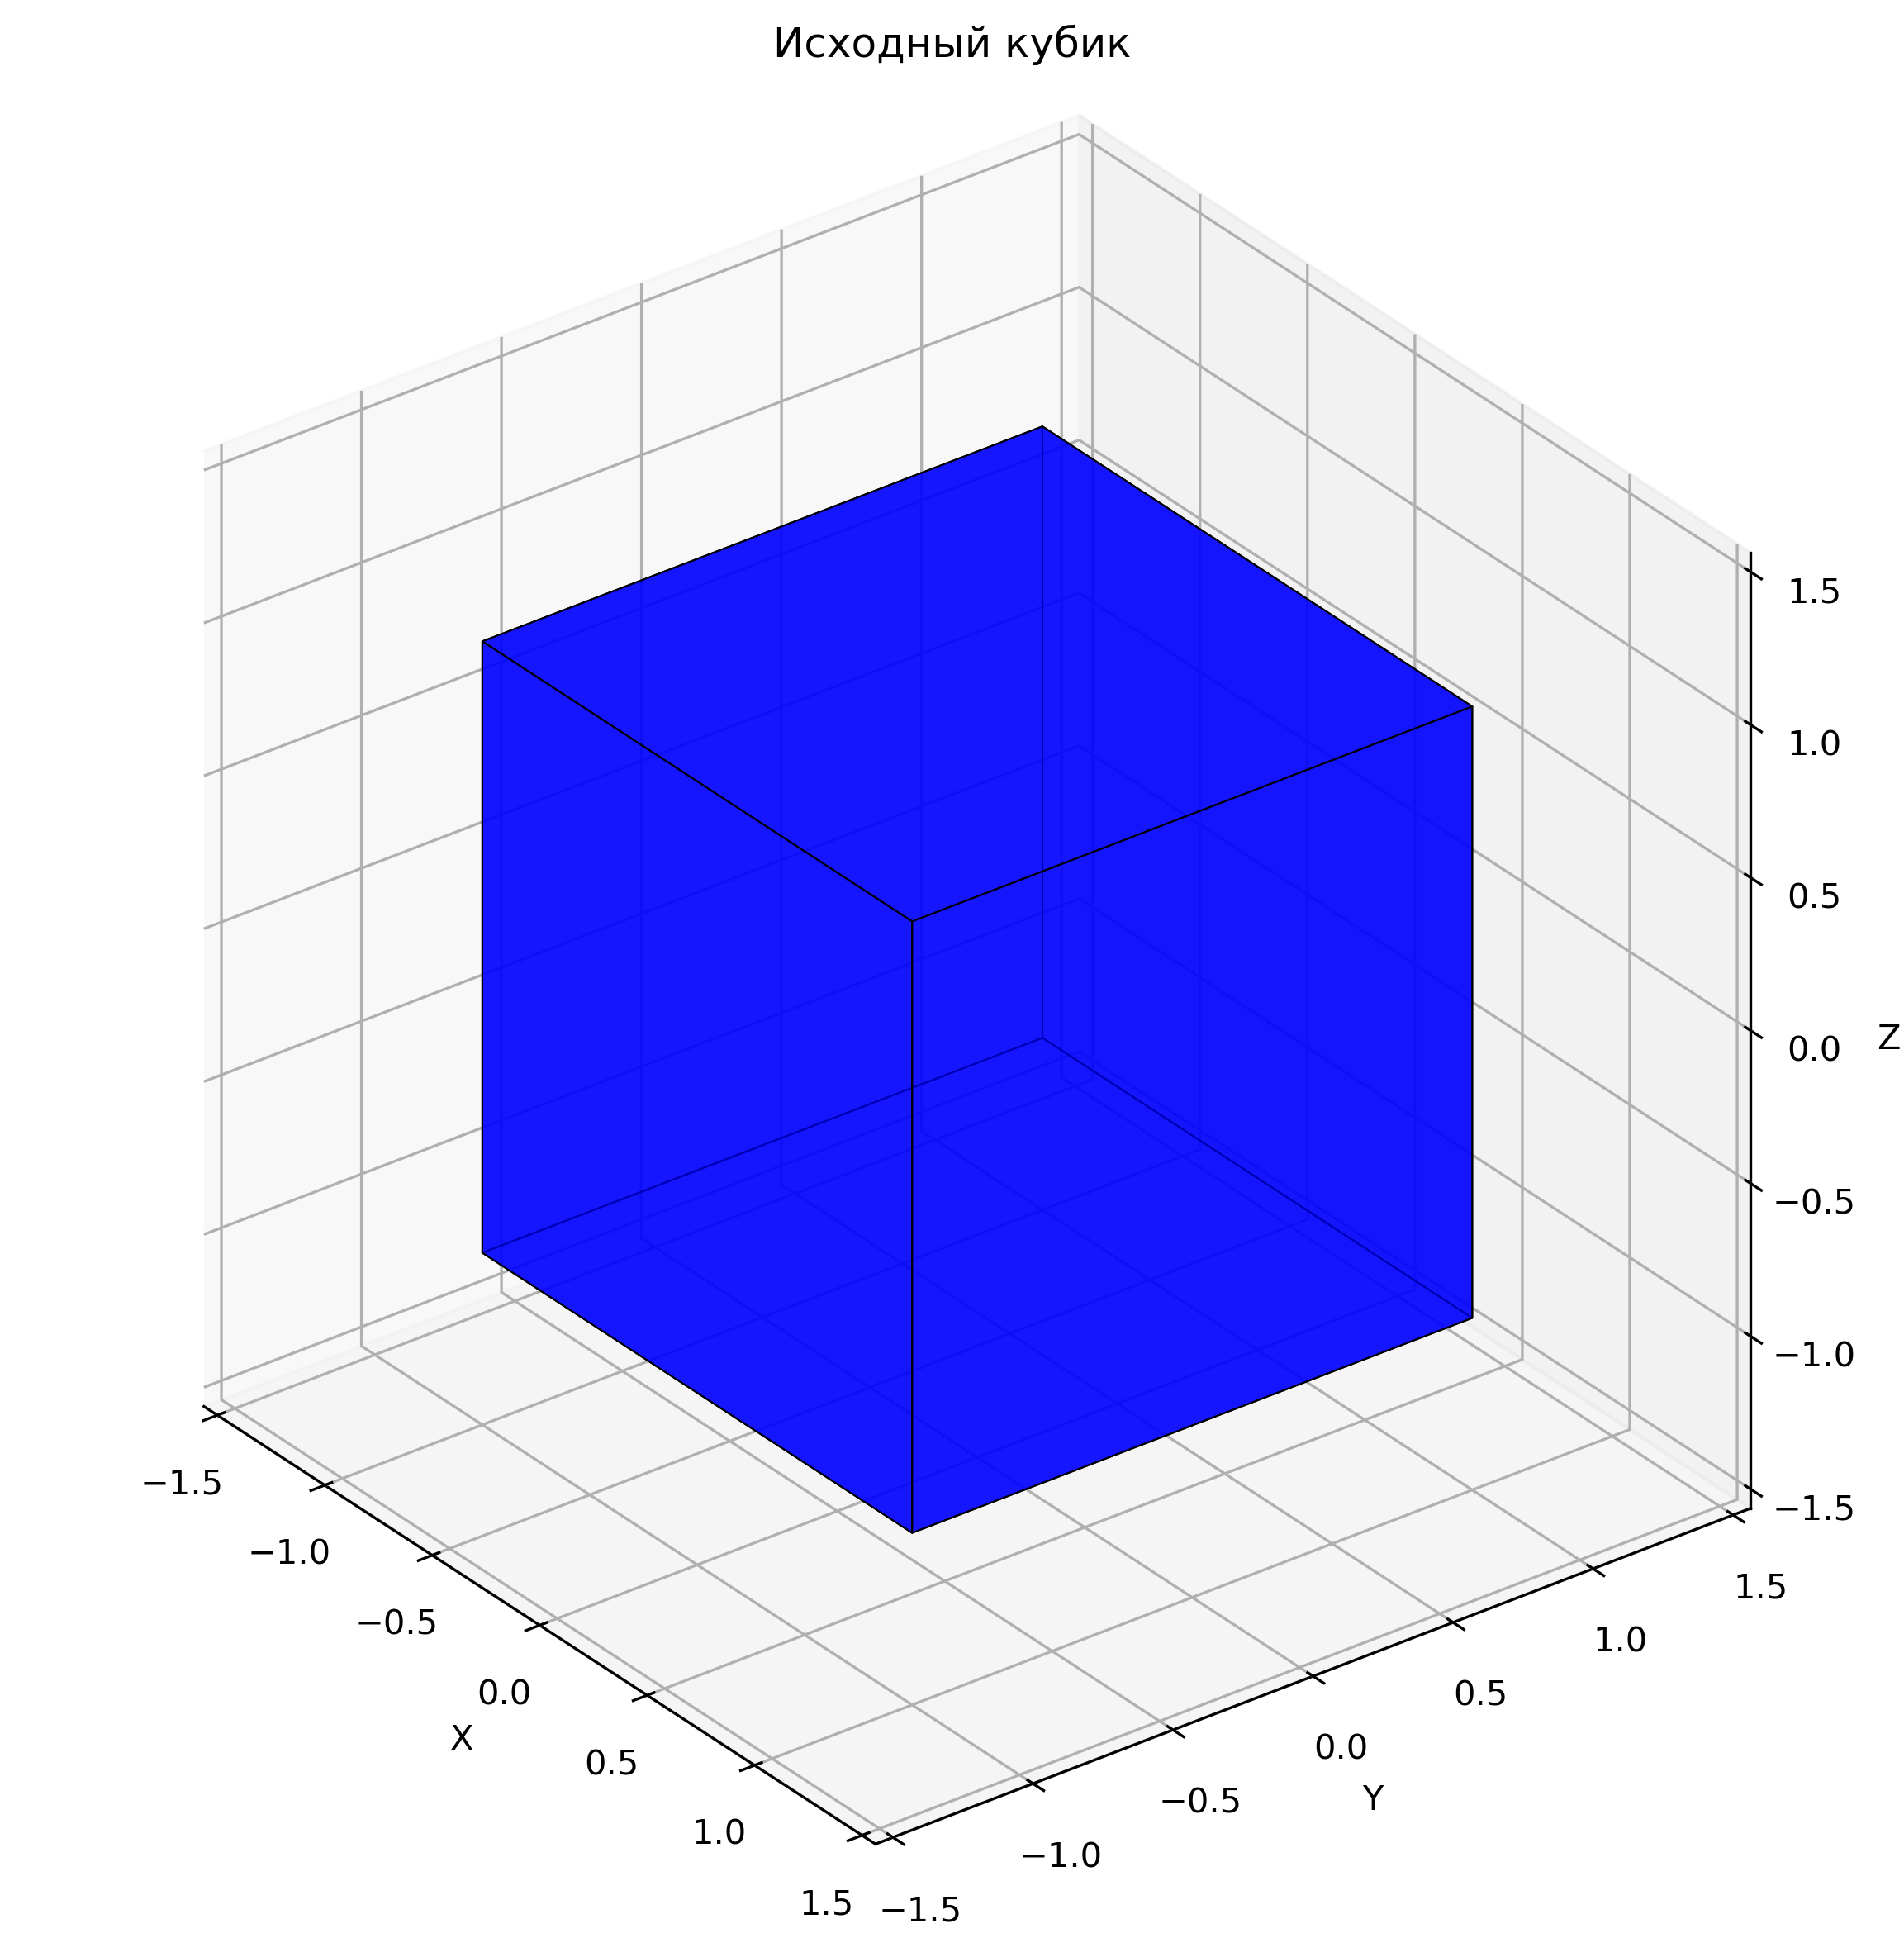
\includegraphics[width=0.8\textwidth]{images/task1/original_cube.png}
\caption{Исходный кубик в однородных координатах}
\end{figure}

\subsection*{Дополнительные фигуры}
Также были созданы тетраэдр и пирамида для демонстрации универсальности подхода.

\begin{figure}[H]
\centering
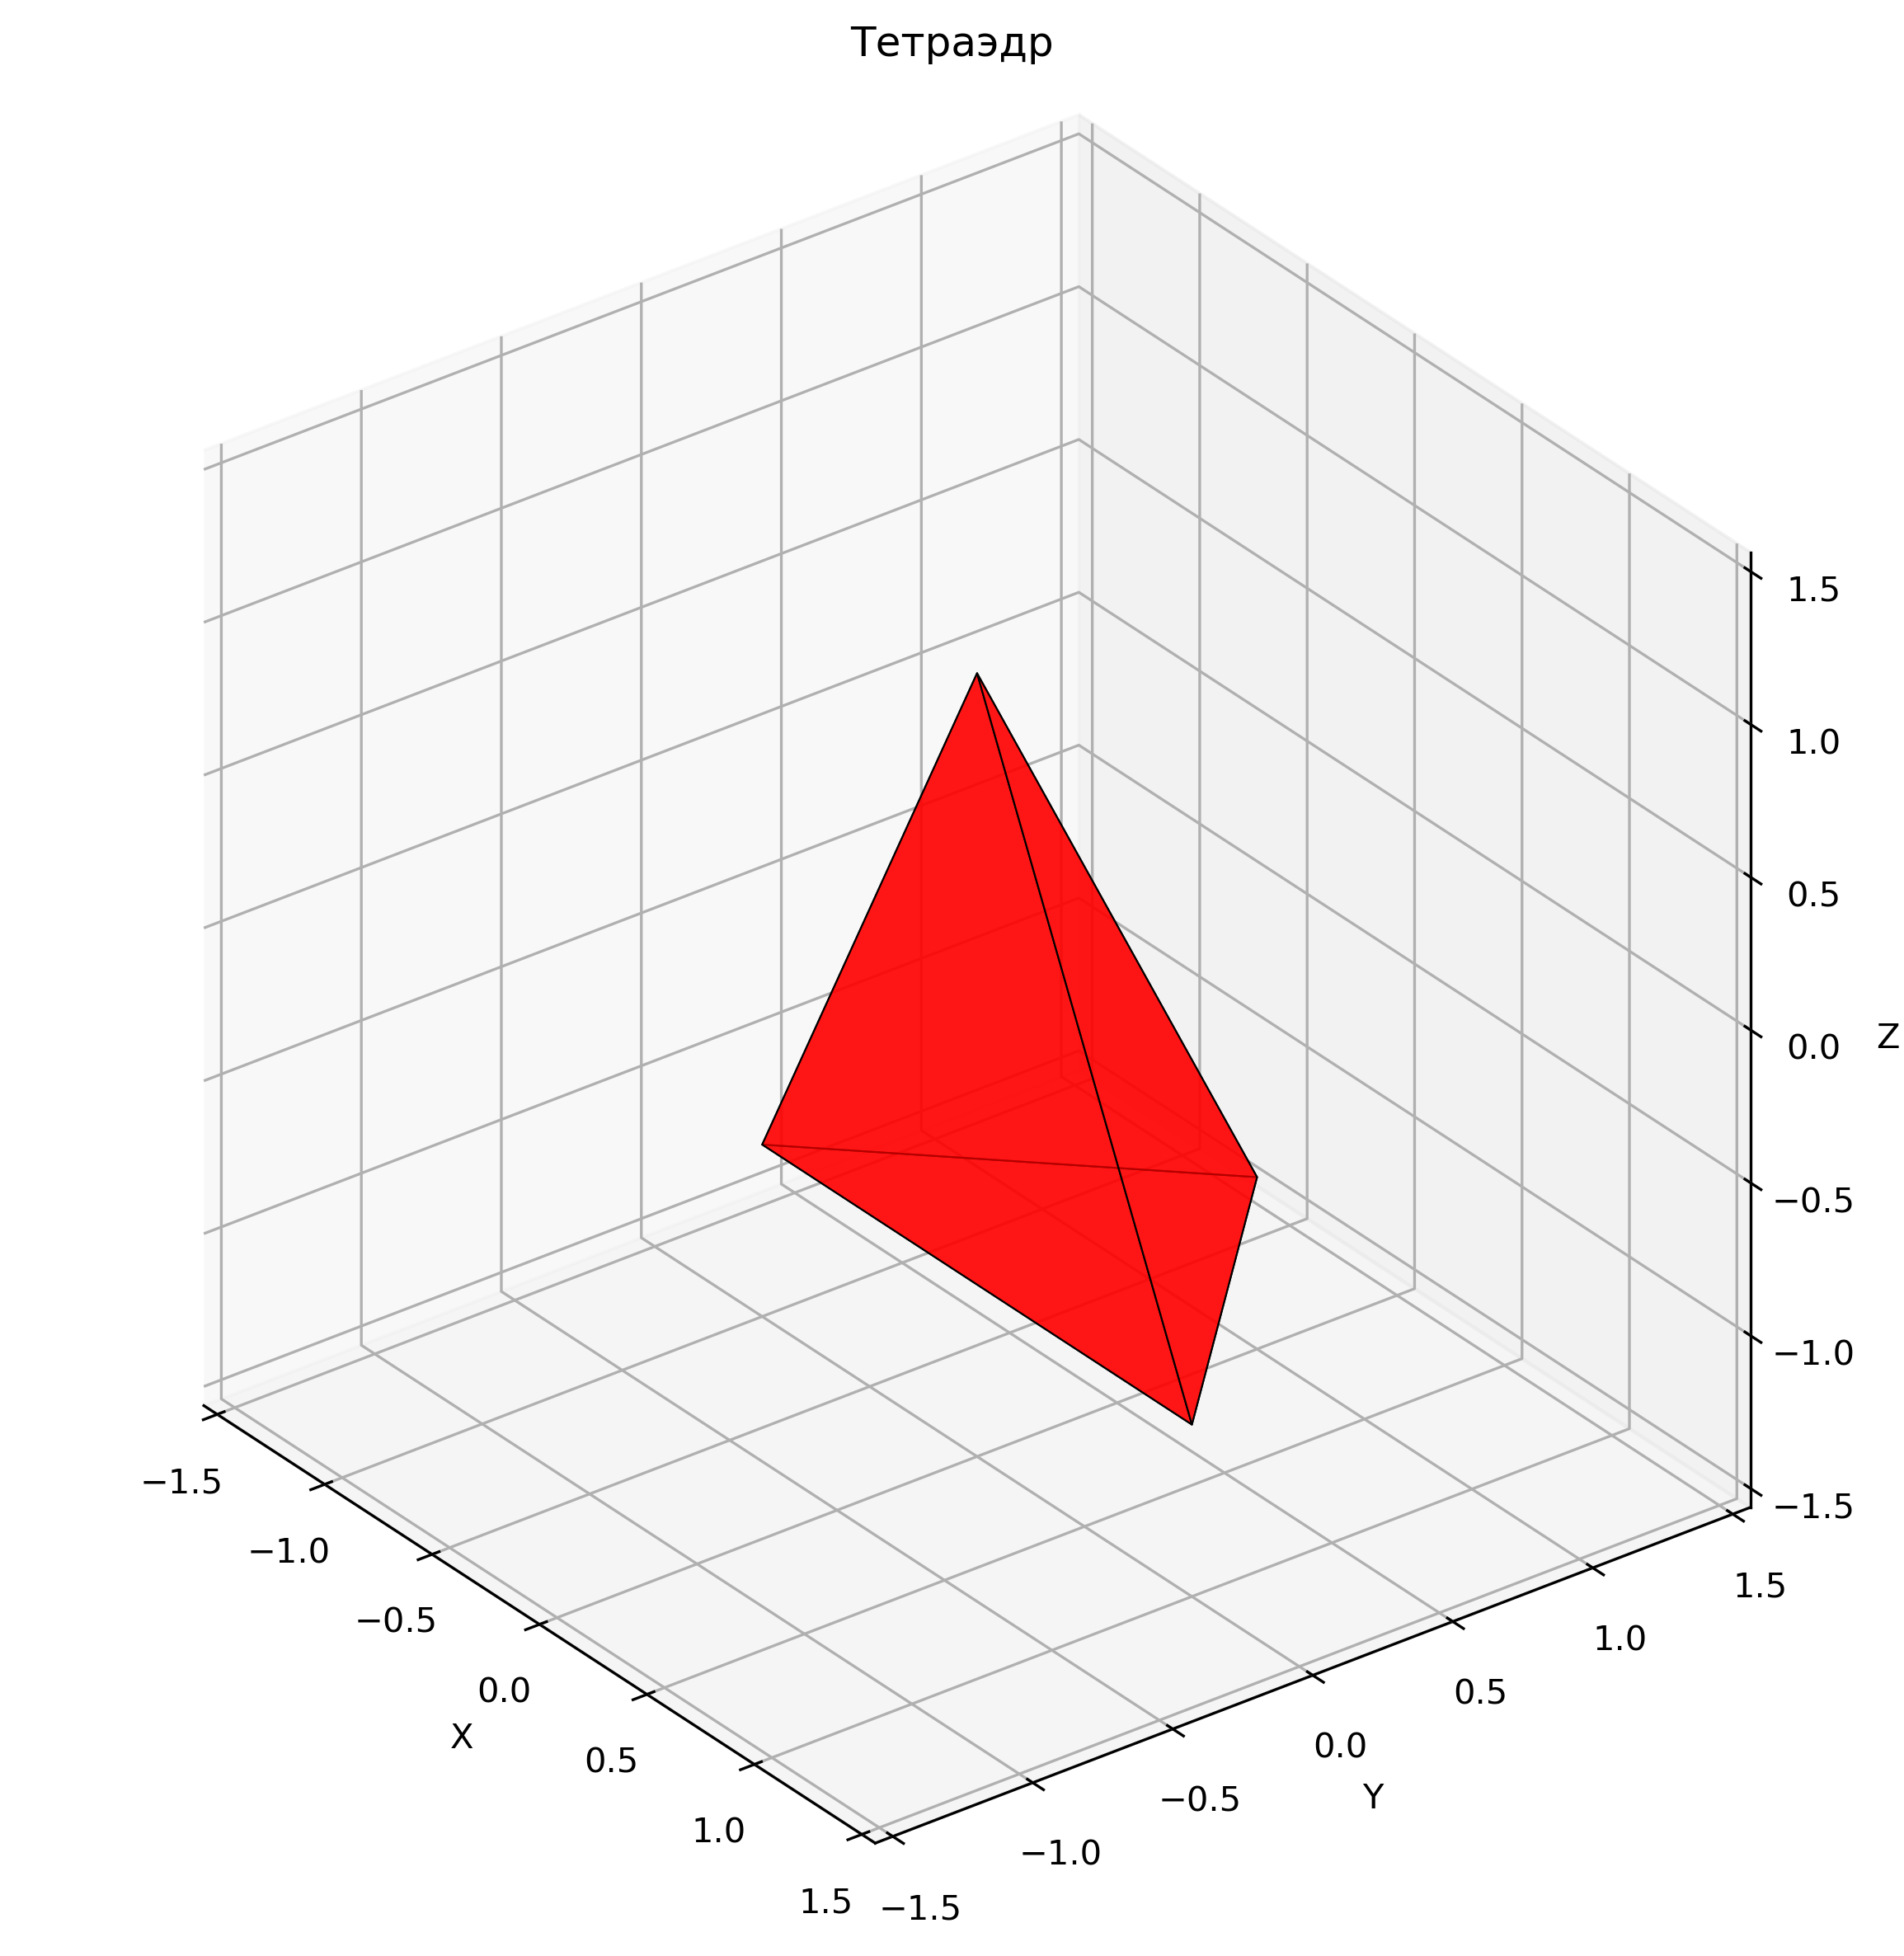
\includegraphics[width=0.8\textwidth]{images/task1/tetrahedron.png}
\caption{Тетраэдр с 4 вершинами и 4 треугольными гранями}
\end{figure}

\begin{figure}[H]
\centering
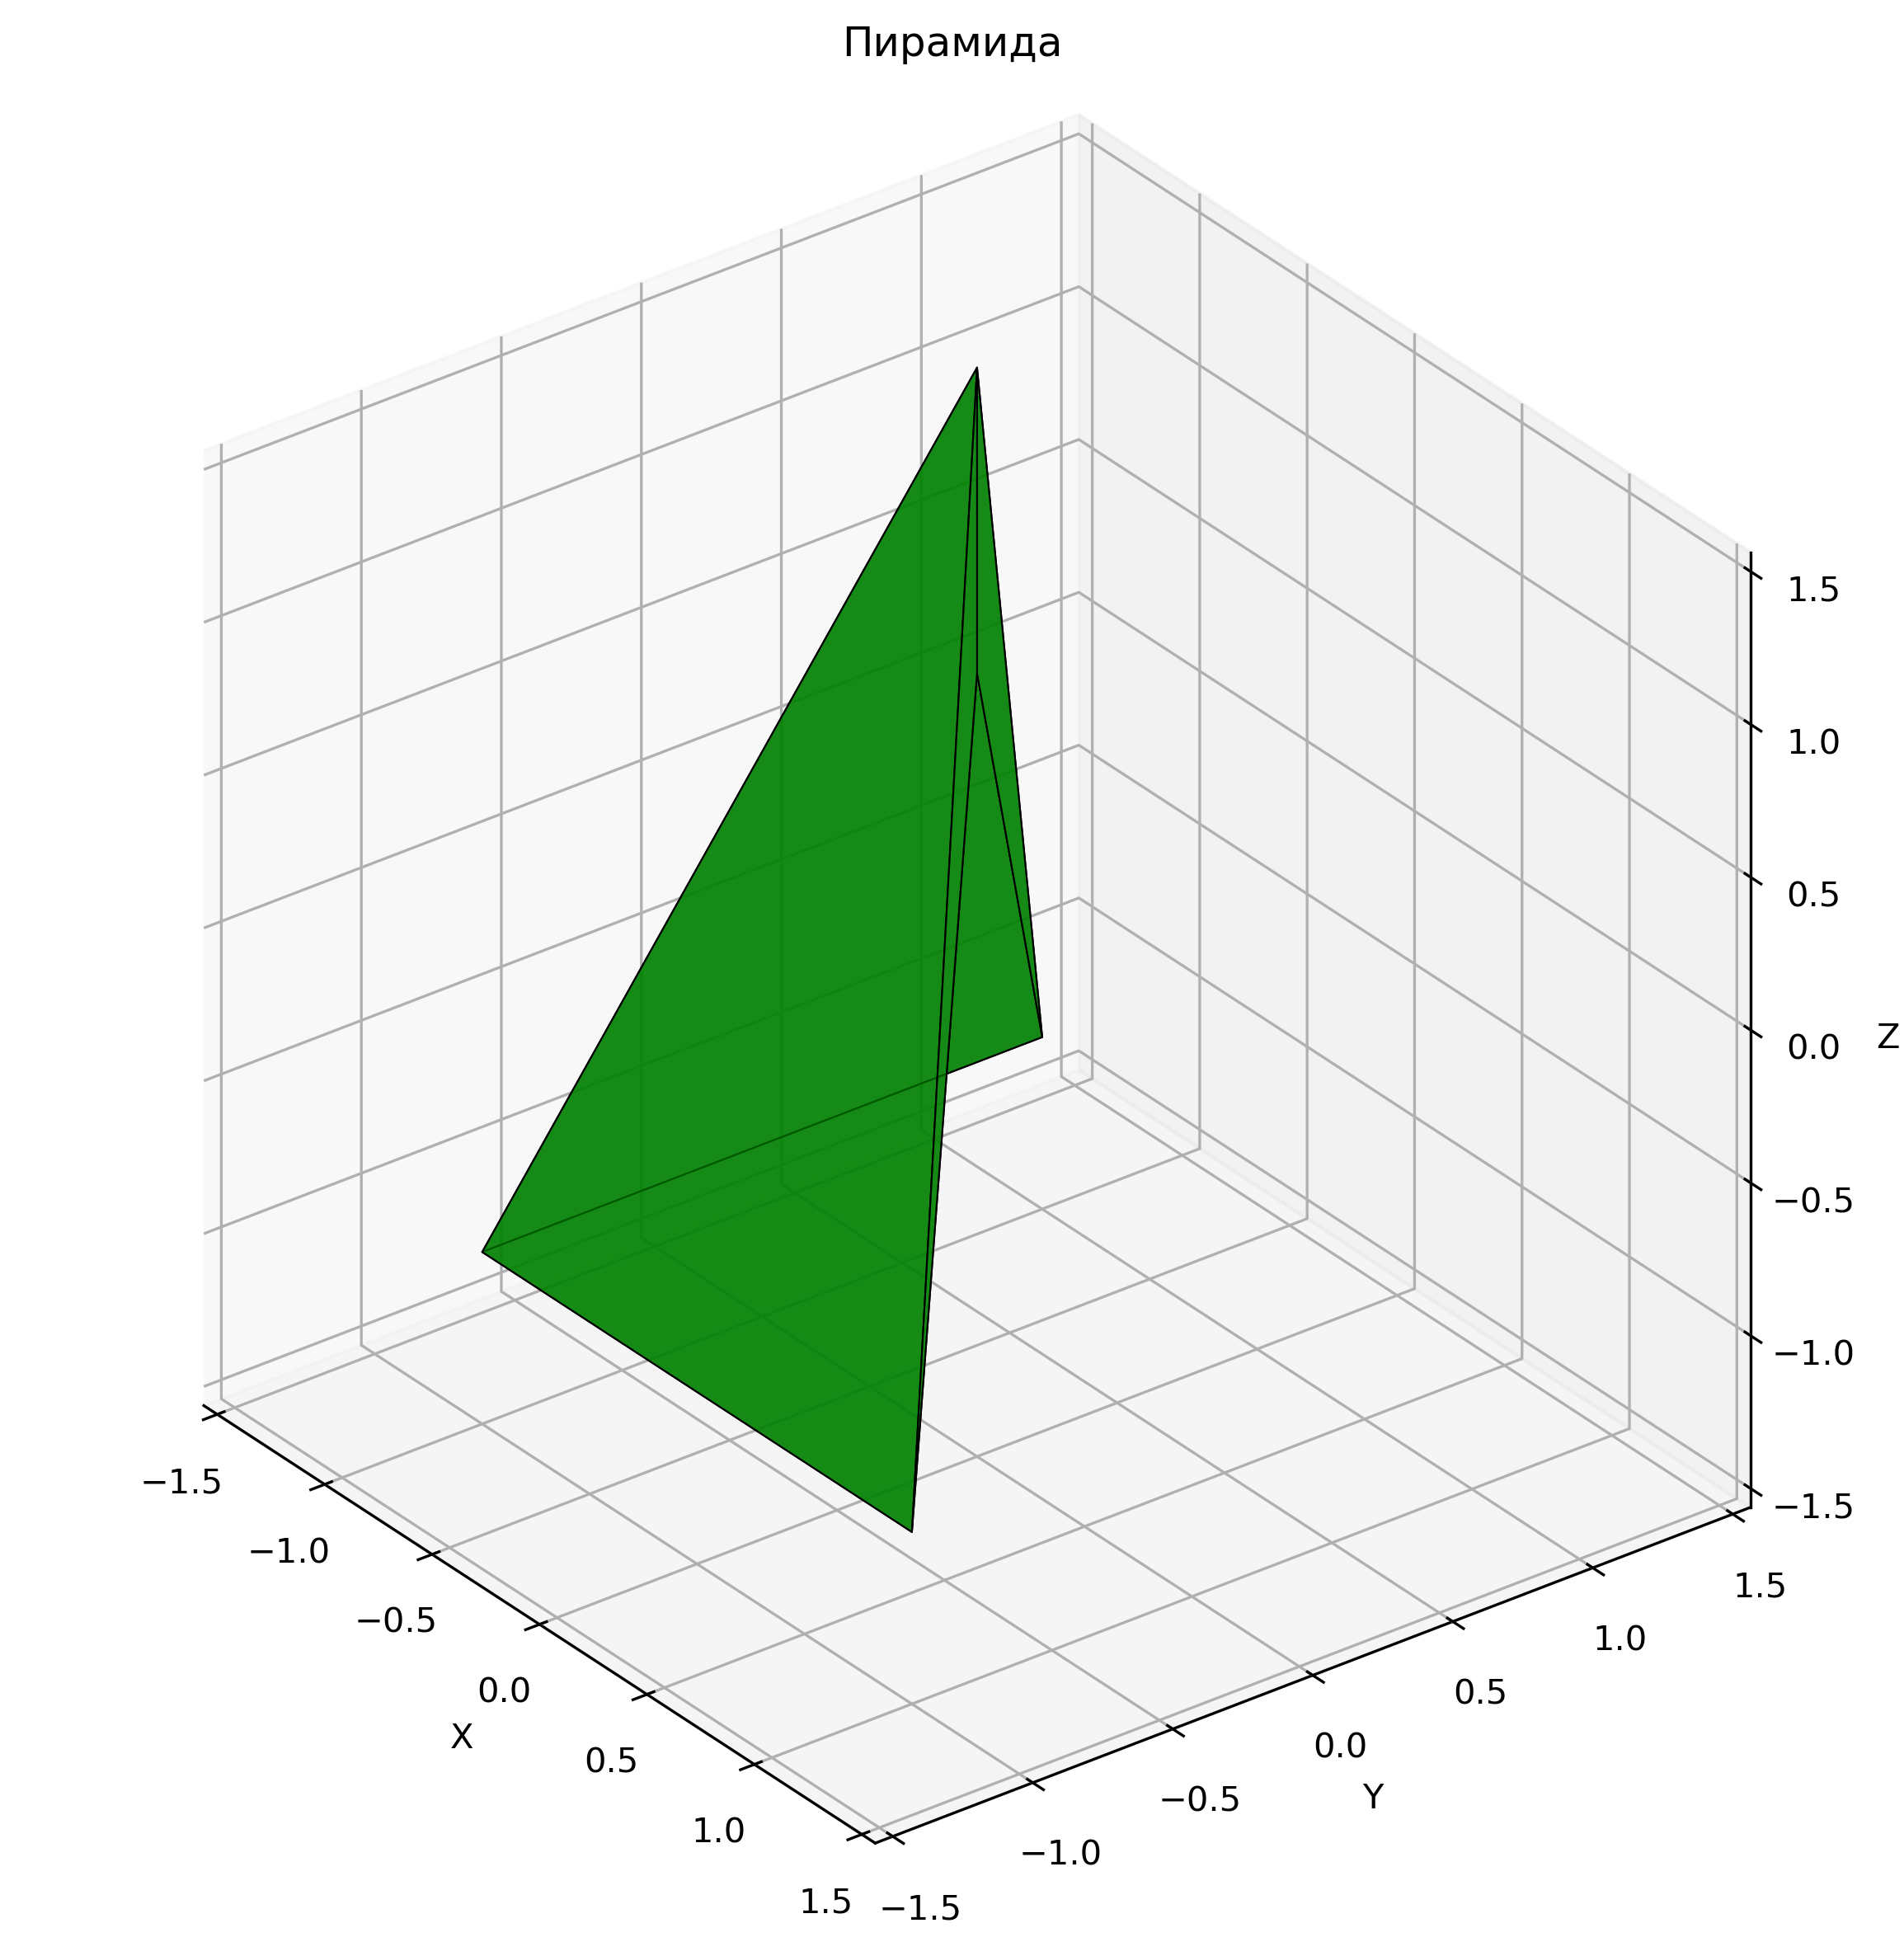
\includegraphics[width=0.8\textwidth]{images/task1/pyramid.png}
\caption{Пирамида с квадратным основанием}
\end{figure}

\section*{Задание 2: Масштабирование кубика}

\subsection*{Постановка задачи}
Исследовать эффекты масштабирования кубика по различным осям и проанализировать свойства матриц масштабирования.

\subsection*{Математические основы}
Матрица масштабирования в однородных координатах:
\begin{equation}
S = \begin{pmatrix}
s_x & 0 & 0 & 0 \\
0 & s_y & 0 & 0 \\
0 & 0 & s_z & 0 \\
0 & 0 & 0 & 1
\end{pmatrix}
\end{equation}

где $s_x, s_y, s_z$ - коэффициенты масштабирования по соответствующим осям.

\subsection*{Результаты}
Исследованы различные случаи масштабирования:

\begin{figure}[H]
\centering
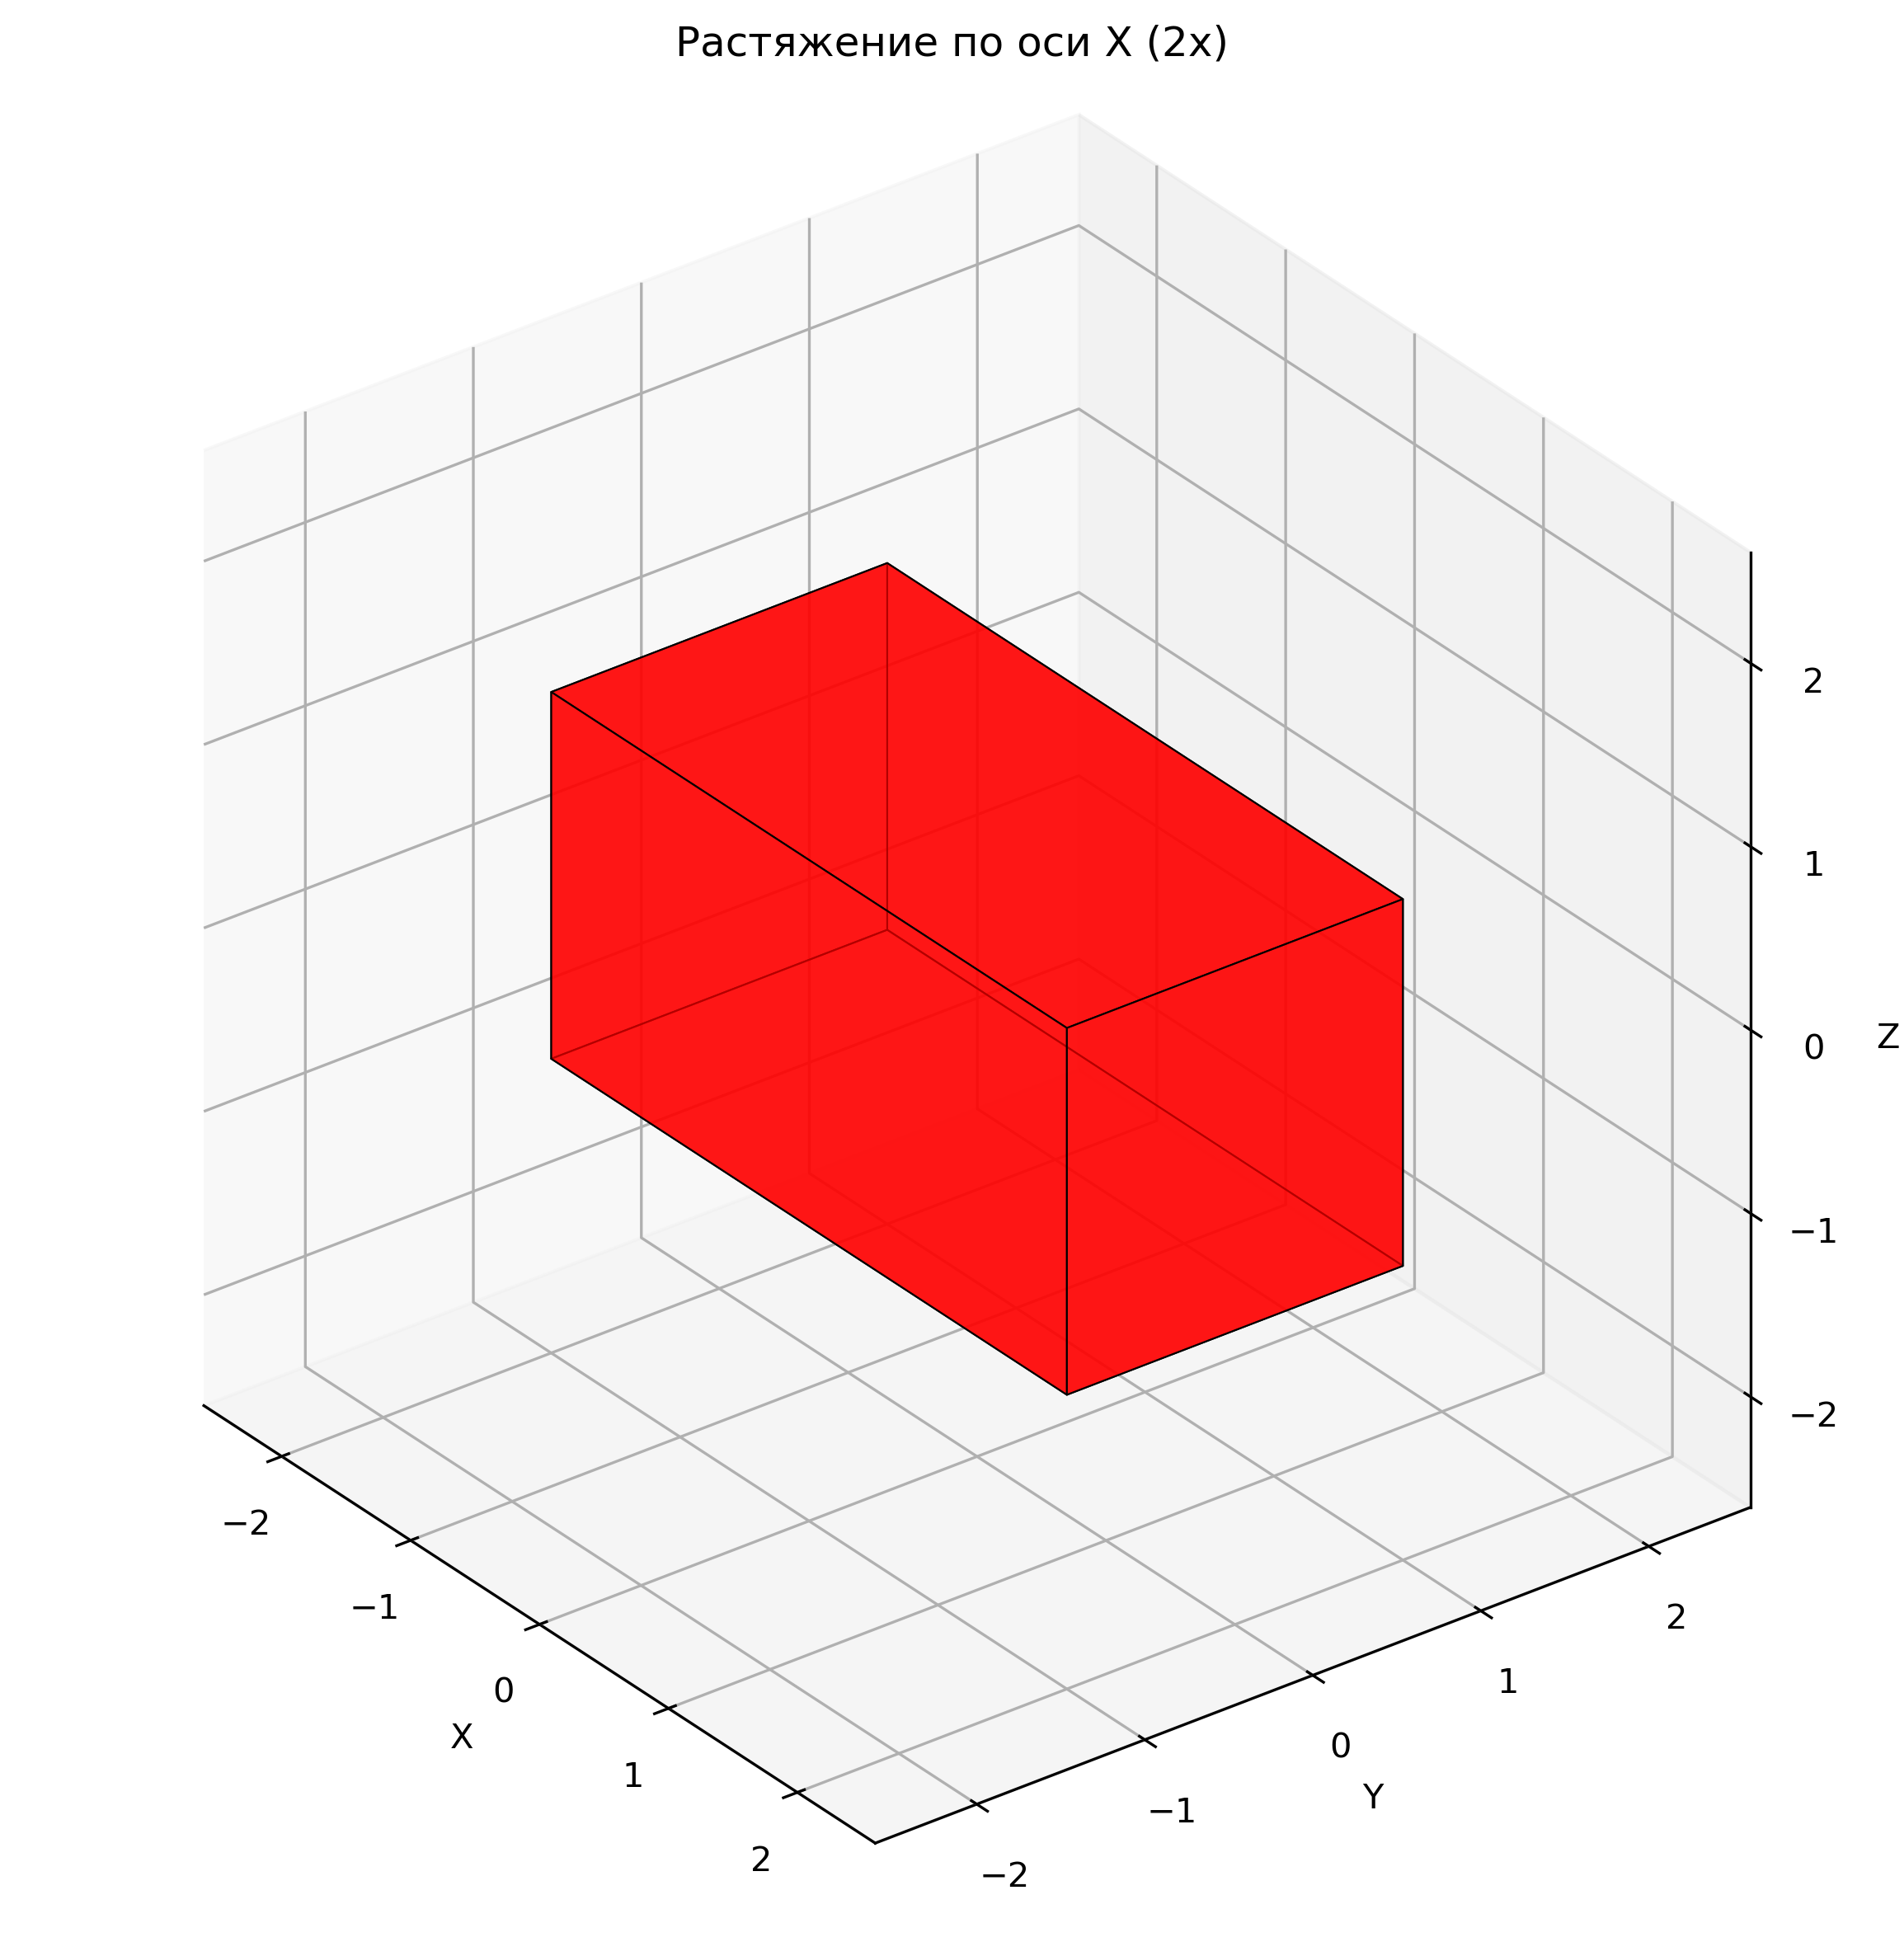
\includegraphics[width=0.8\textwidth]{images/task2/scale_x.png}
\caption{Растяжение по оси X (2x)}
\end{figure}

\begin{figure}[H]
\centering
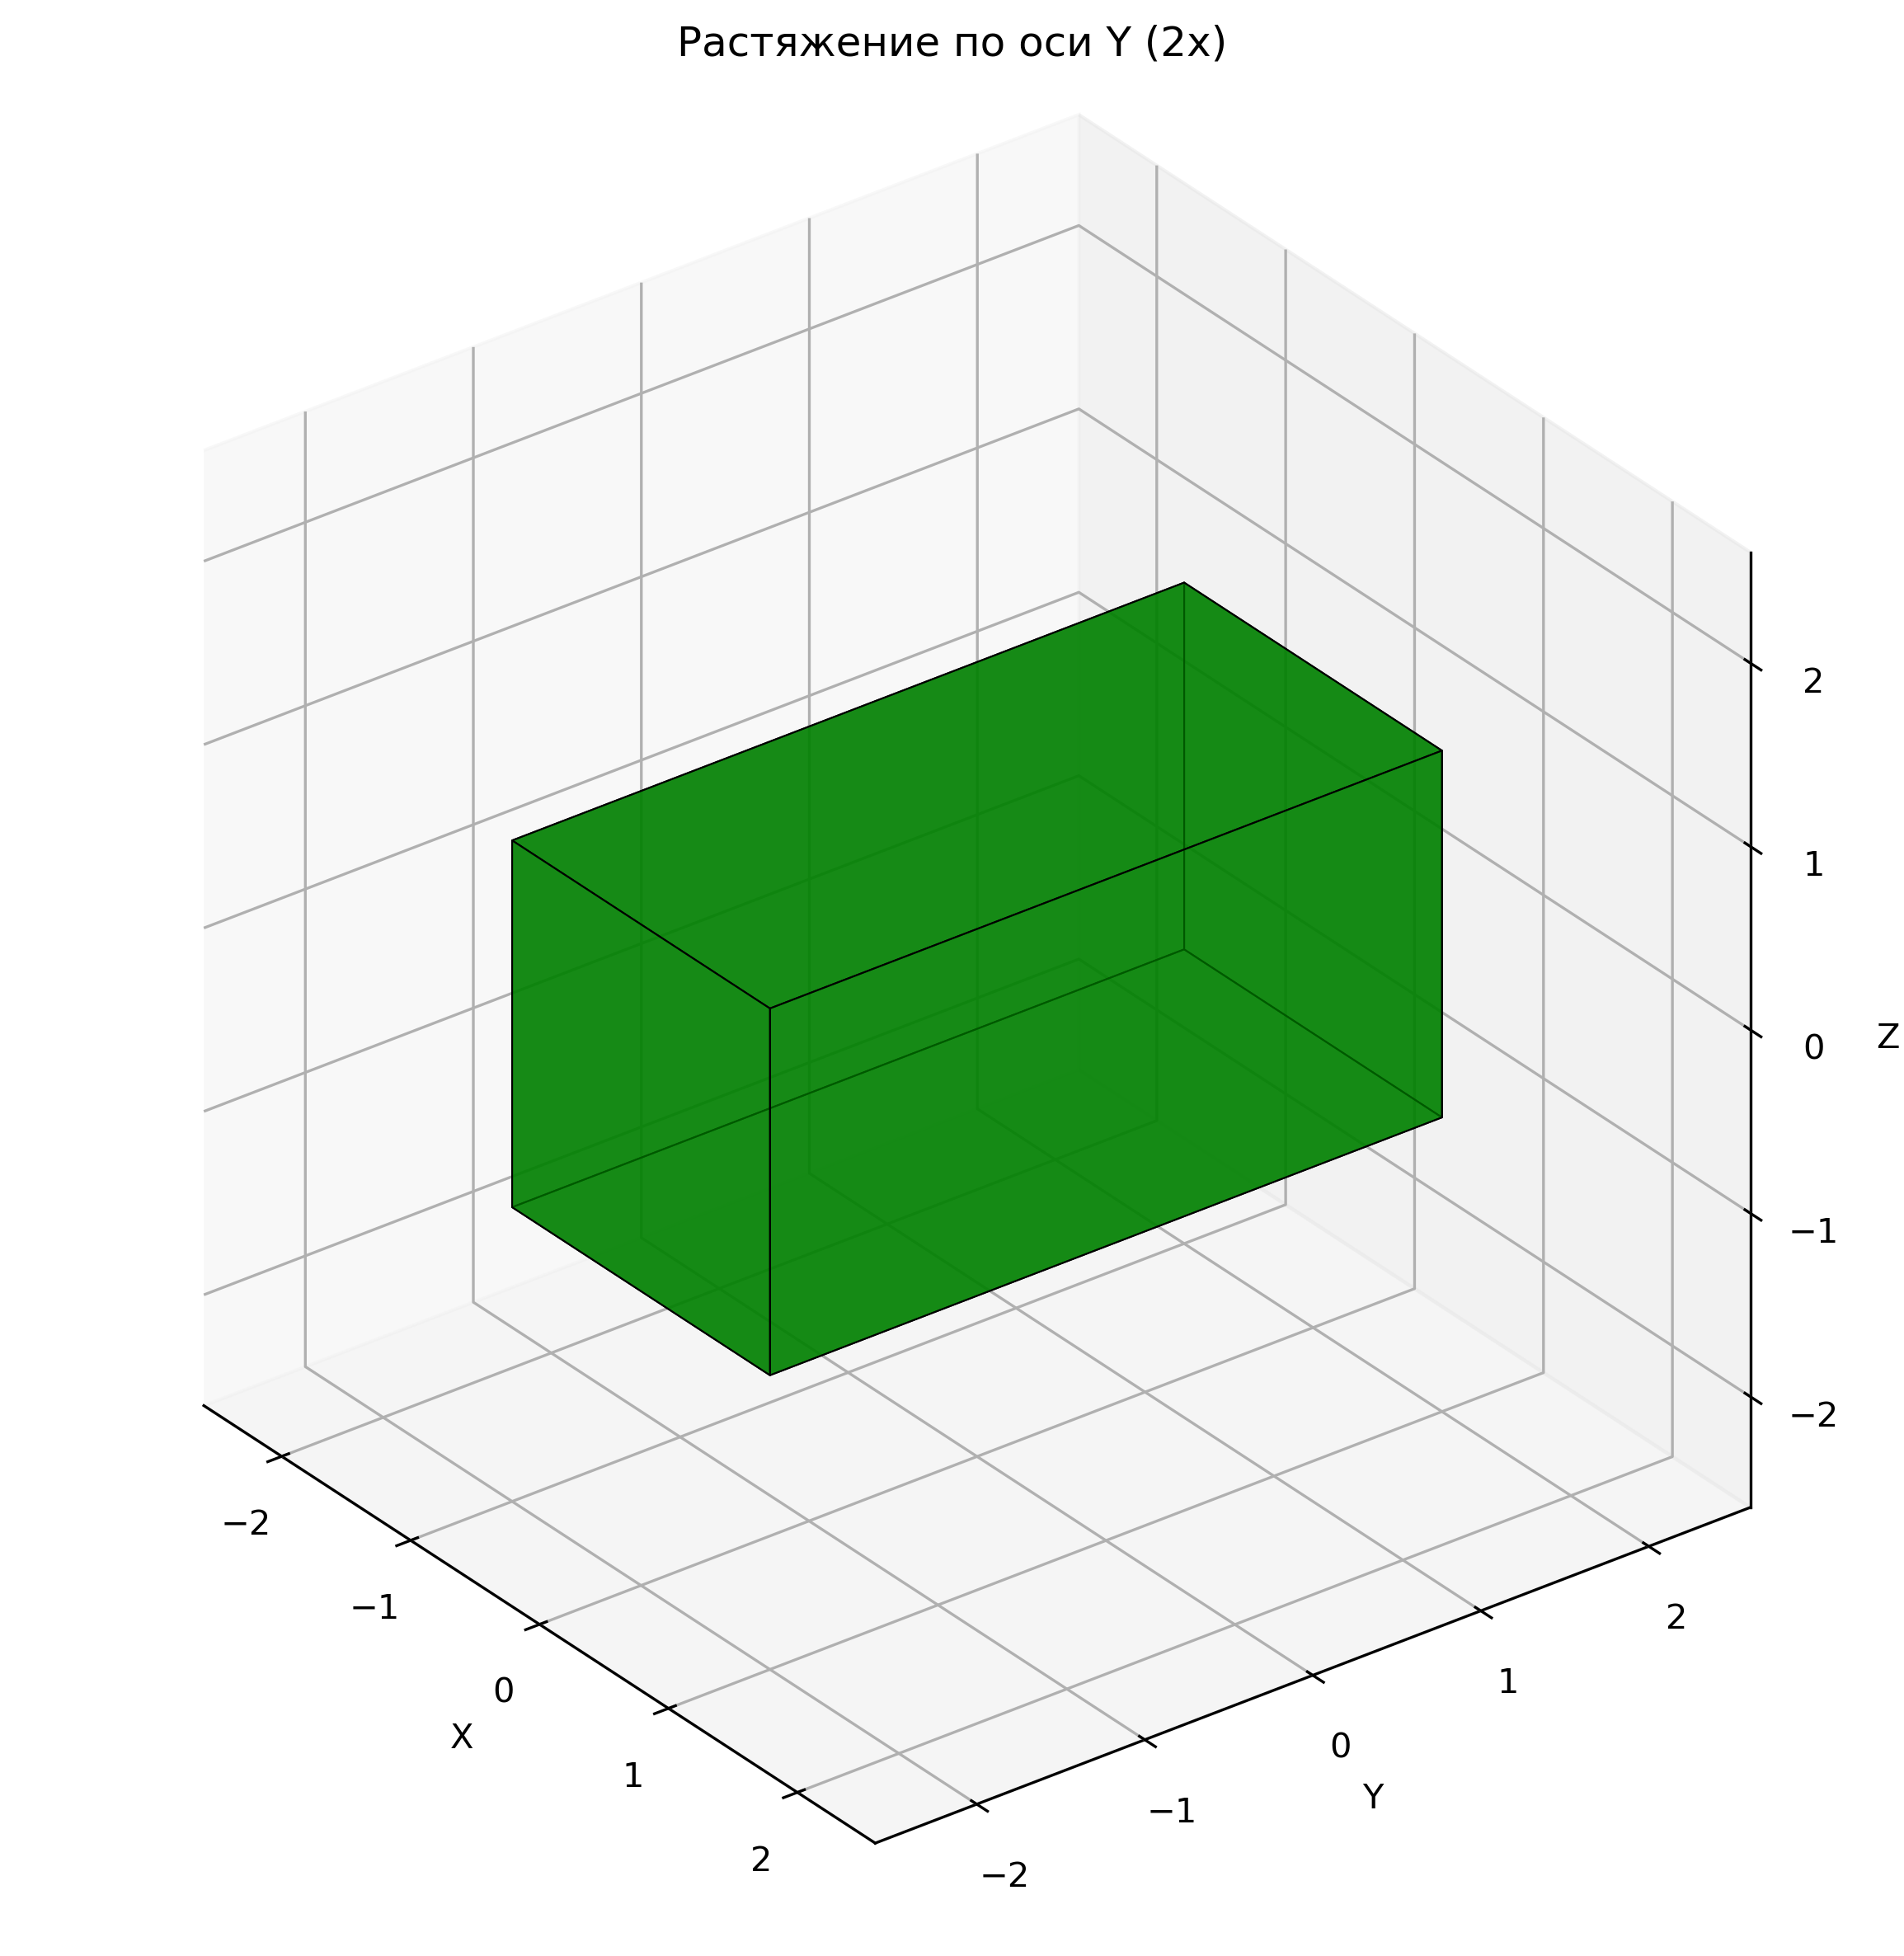
\includegraphics[width=0.8\textwidth]{images/task2/scale_y.png}
\caption{Растяжение по оси Y (2x)}
\end{figure}

\begin{figure}[H]
\centering
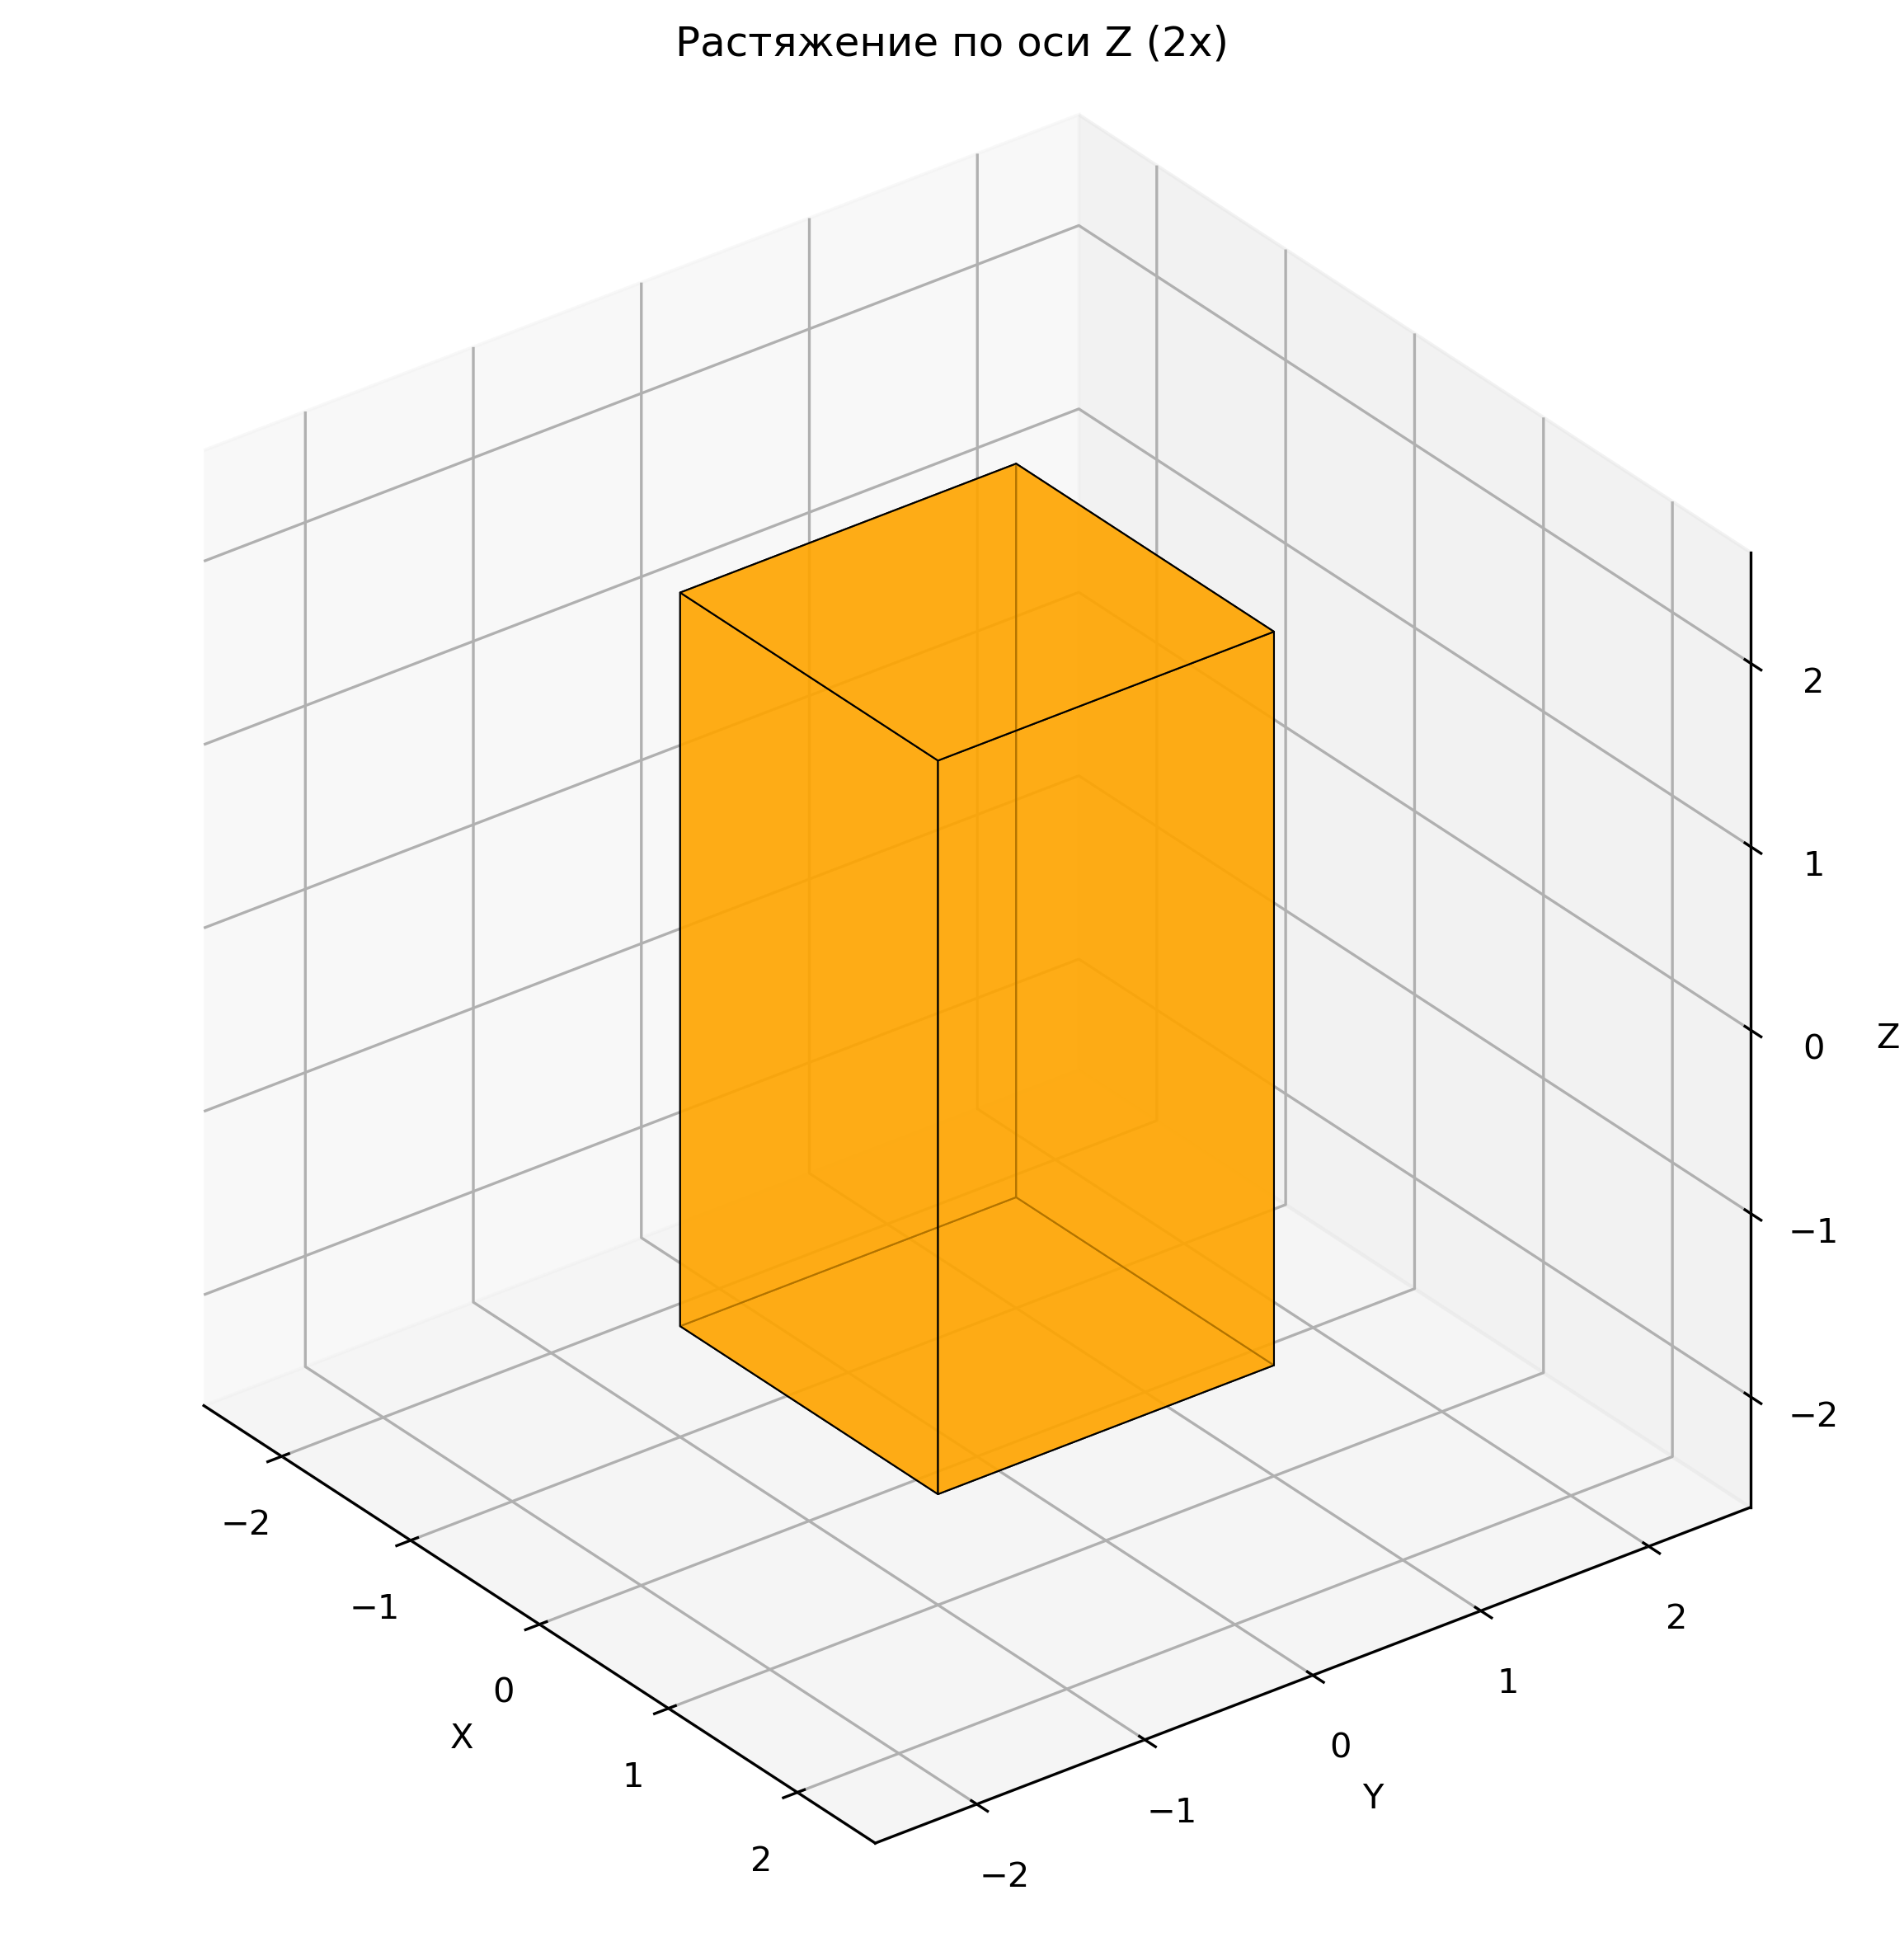
\includegraphics[width=0.8\textwidth]{images/task2/scale_z.png}
\caption{Растяжение по оси Z (2x)}
\end{figure}

\begin{figure}[H]
\centering
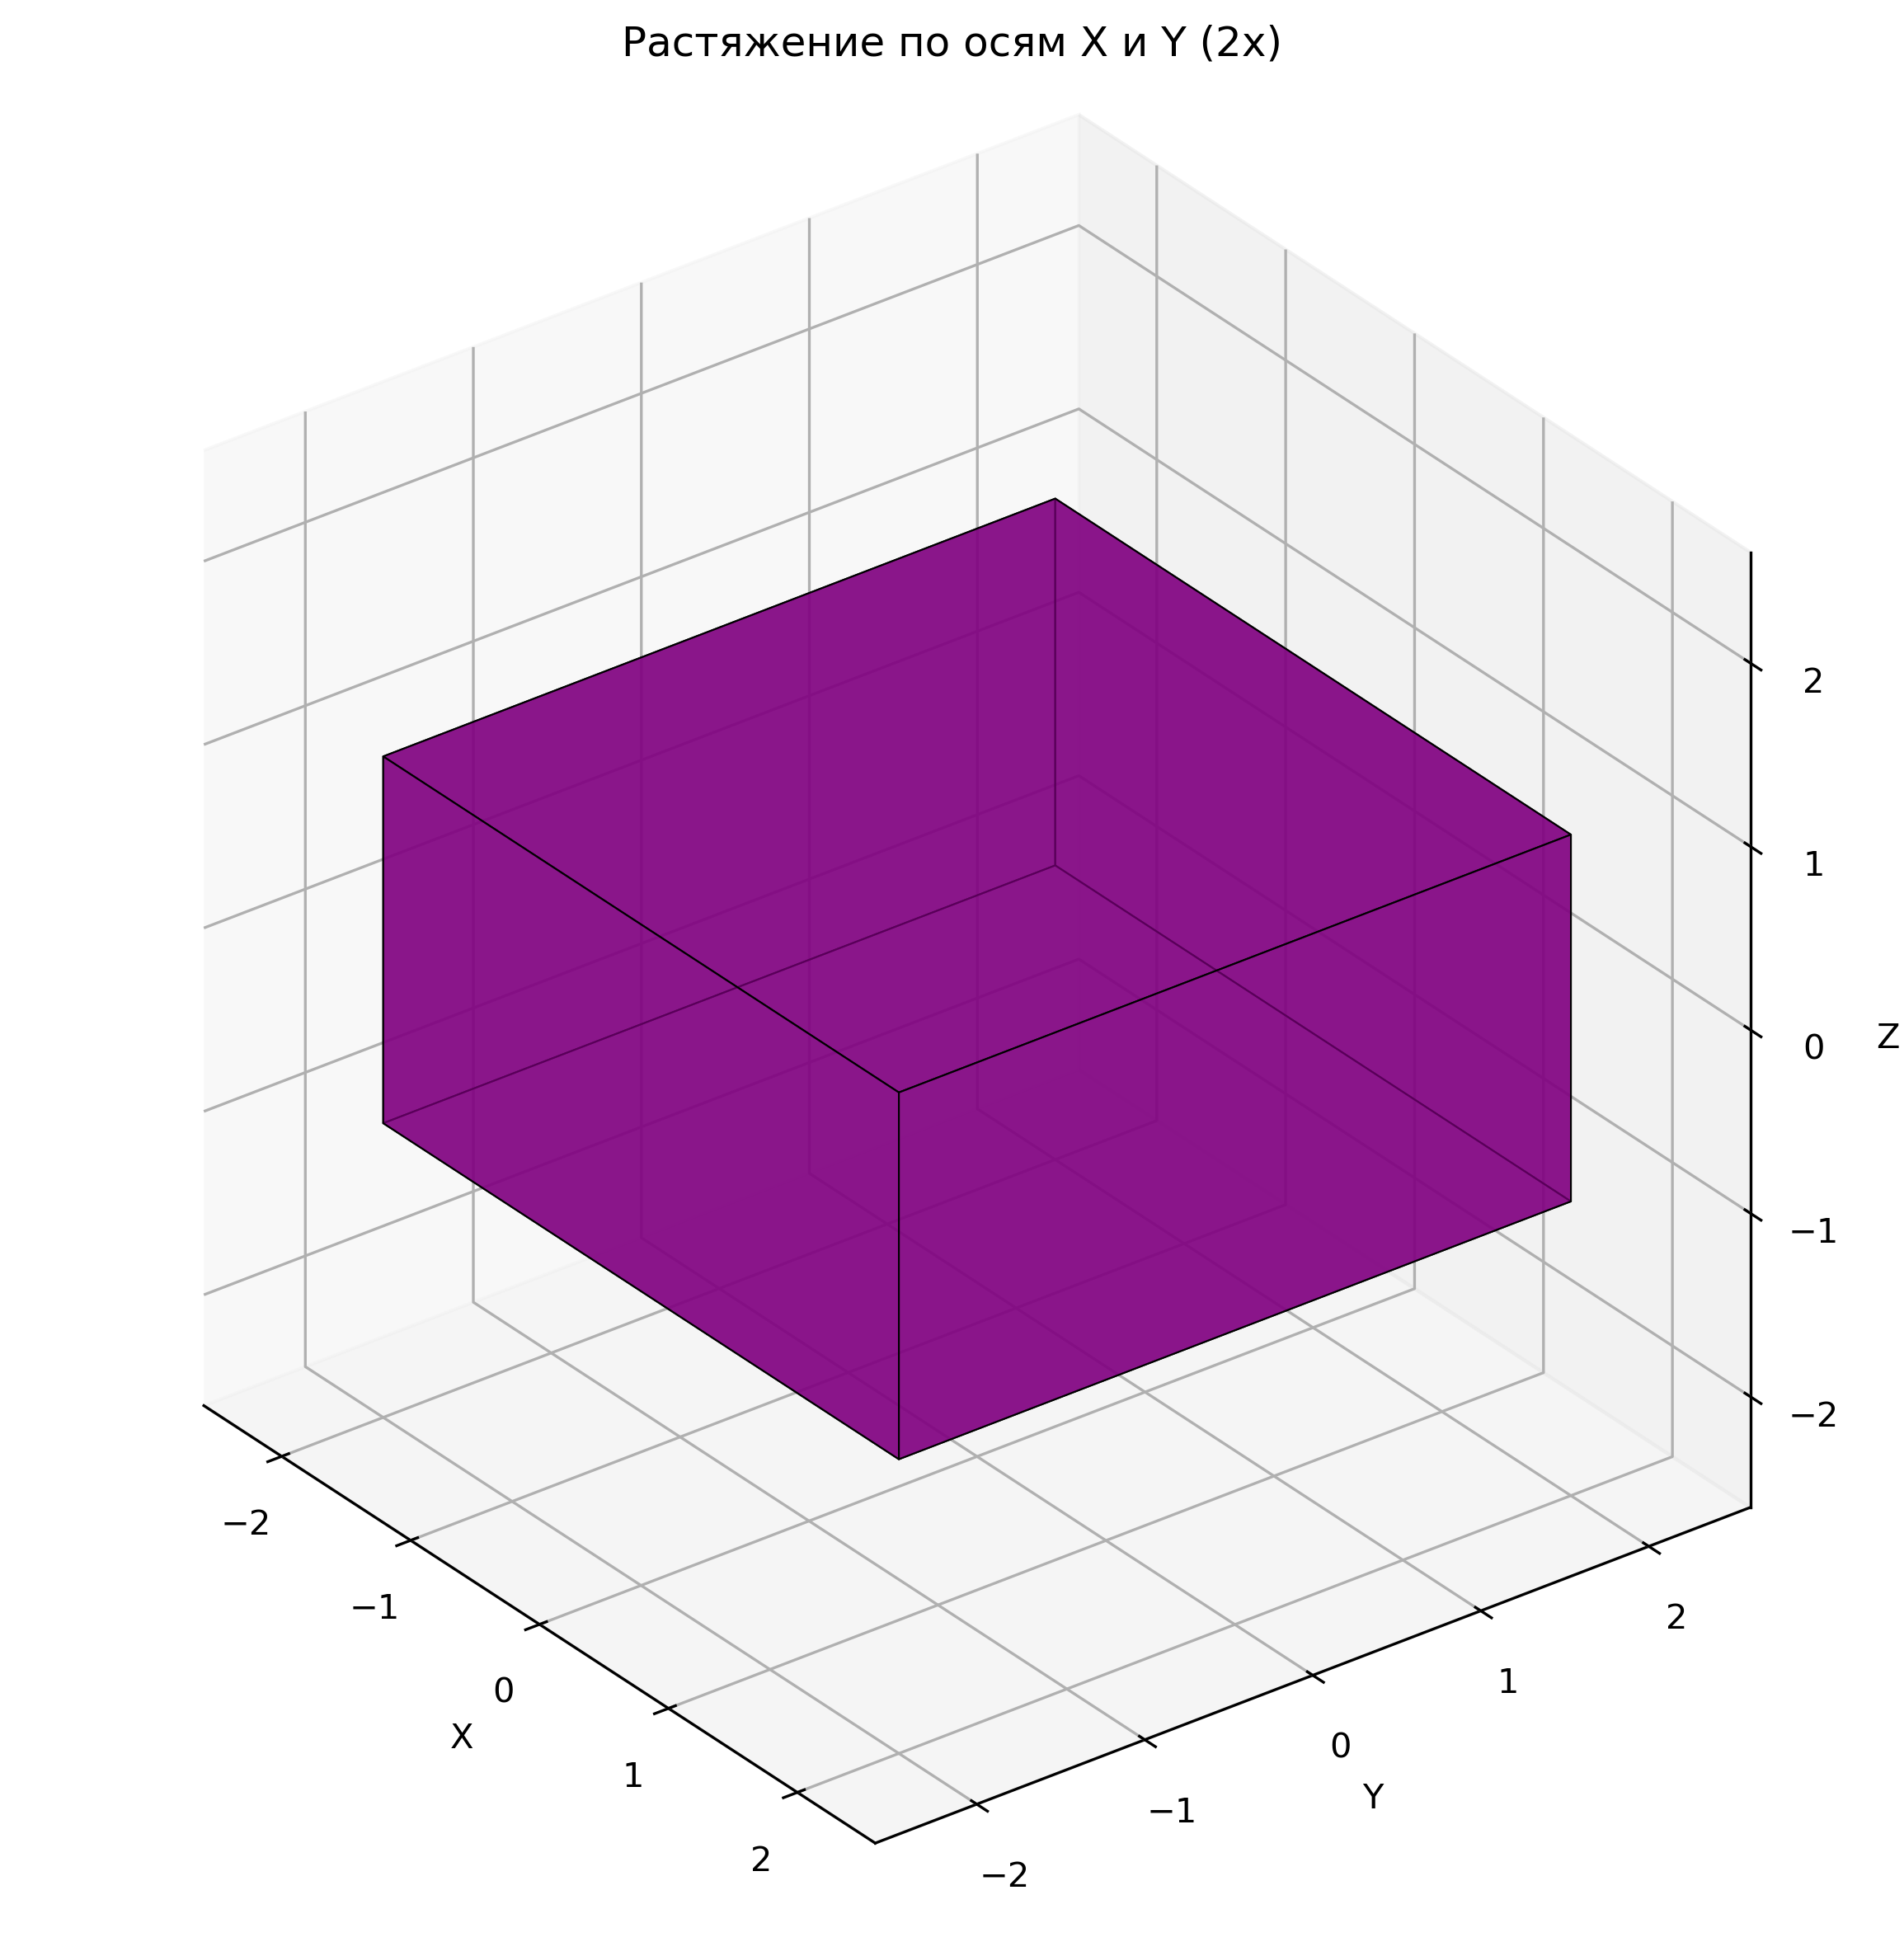
\includegraphics[width=0.8\textwidth]{images/task2/scale_xy.png}
\caption{Растяжение по осям X и Y (2x)}
\end{figure}

\begin{figure}[H]
\centering
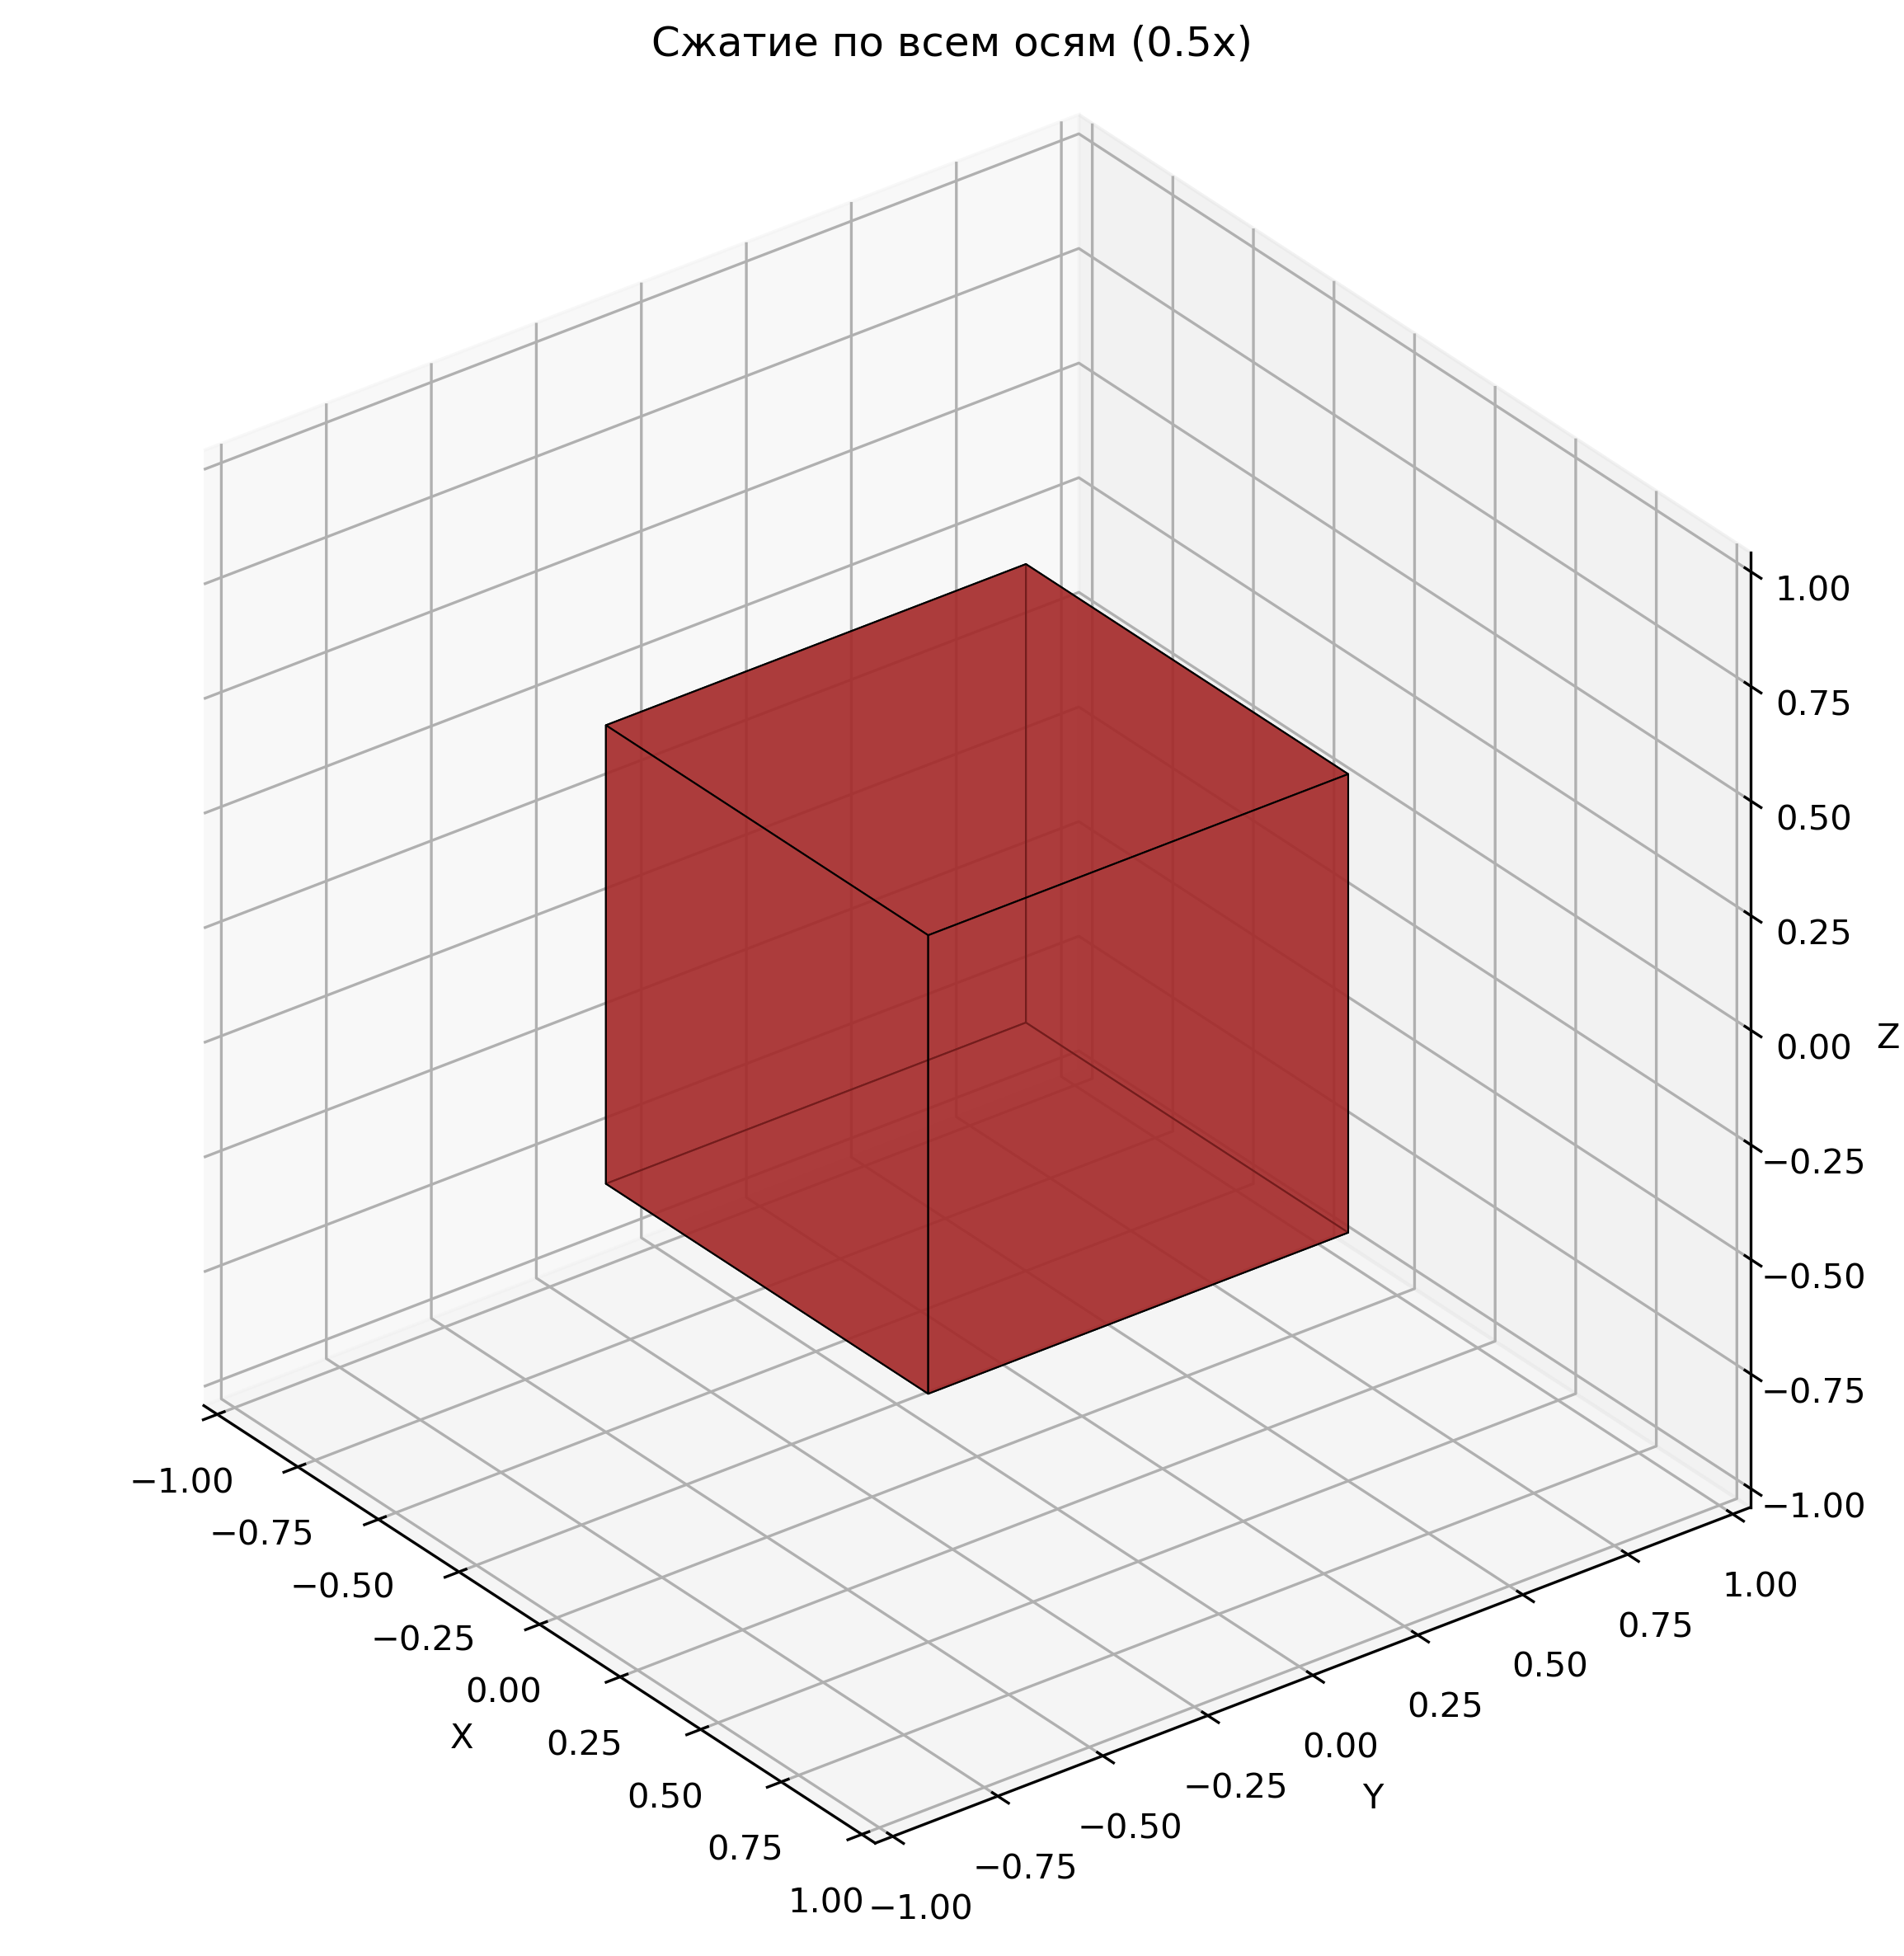
\includegraphics[width=0.8\textwidth]{images/task2/scale_all_small.png}
\caption{Сжатие по всем осям (0.5x)}
\end{figure}

\begin{figure}[H]
\centering
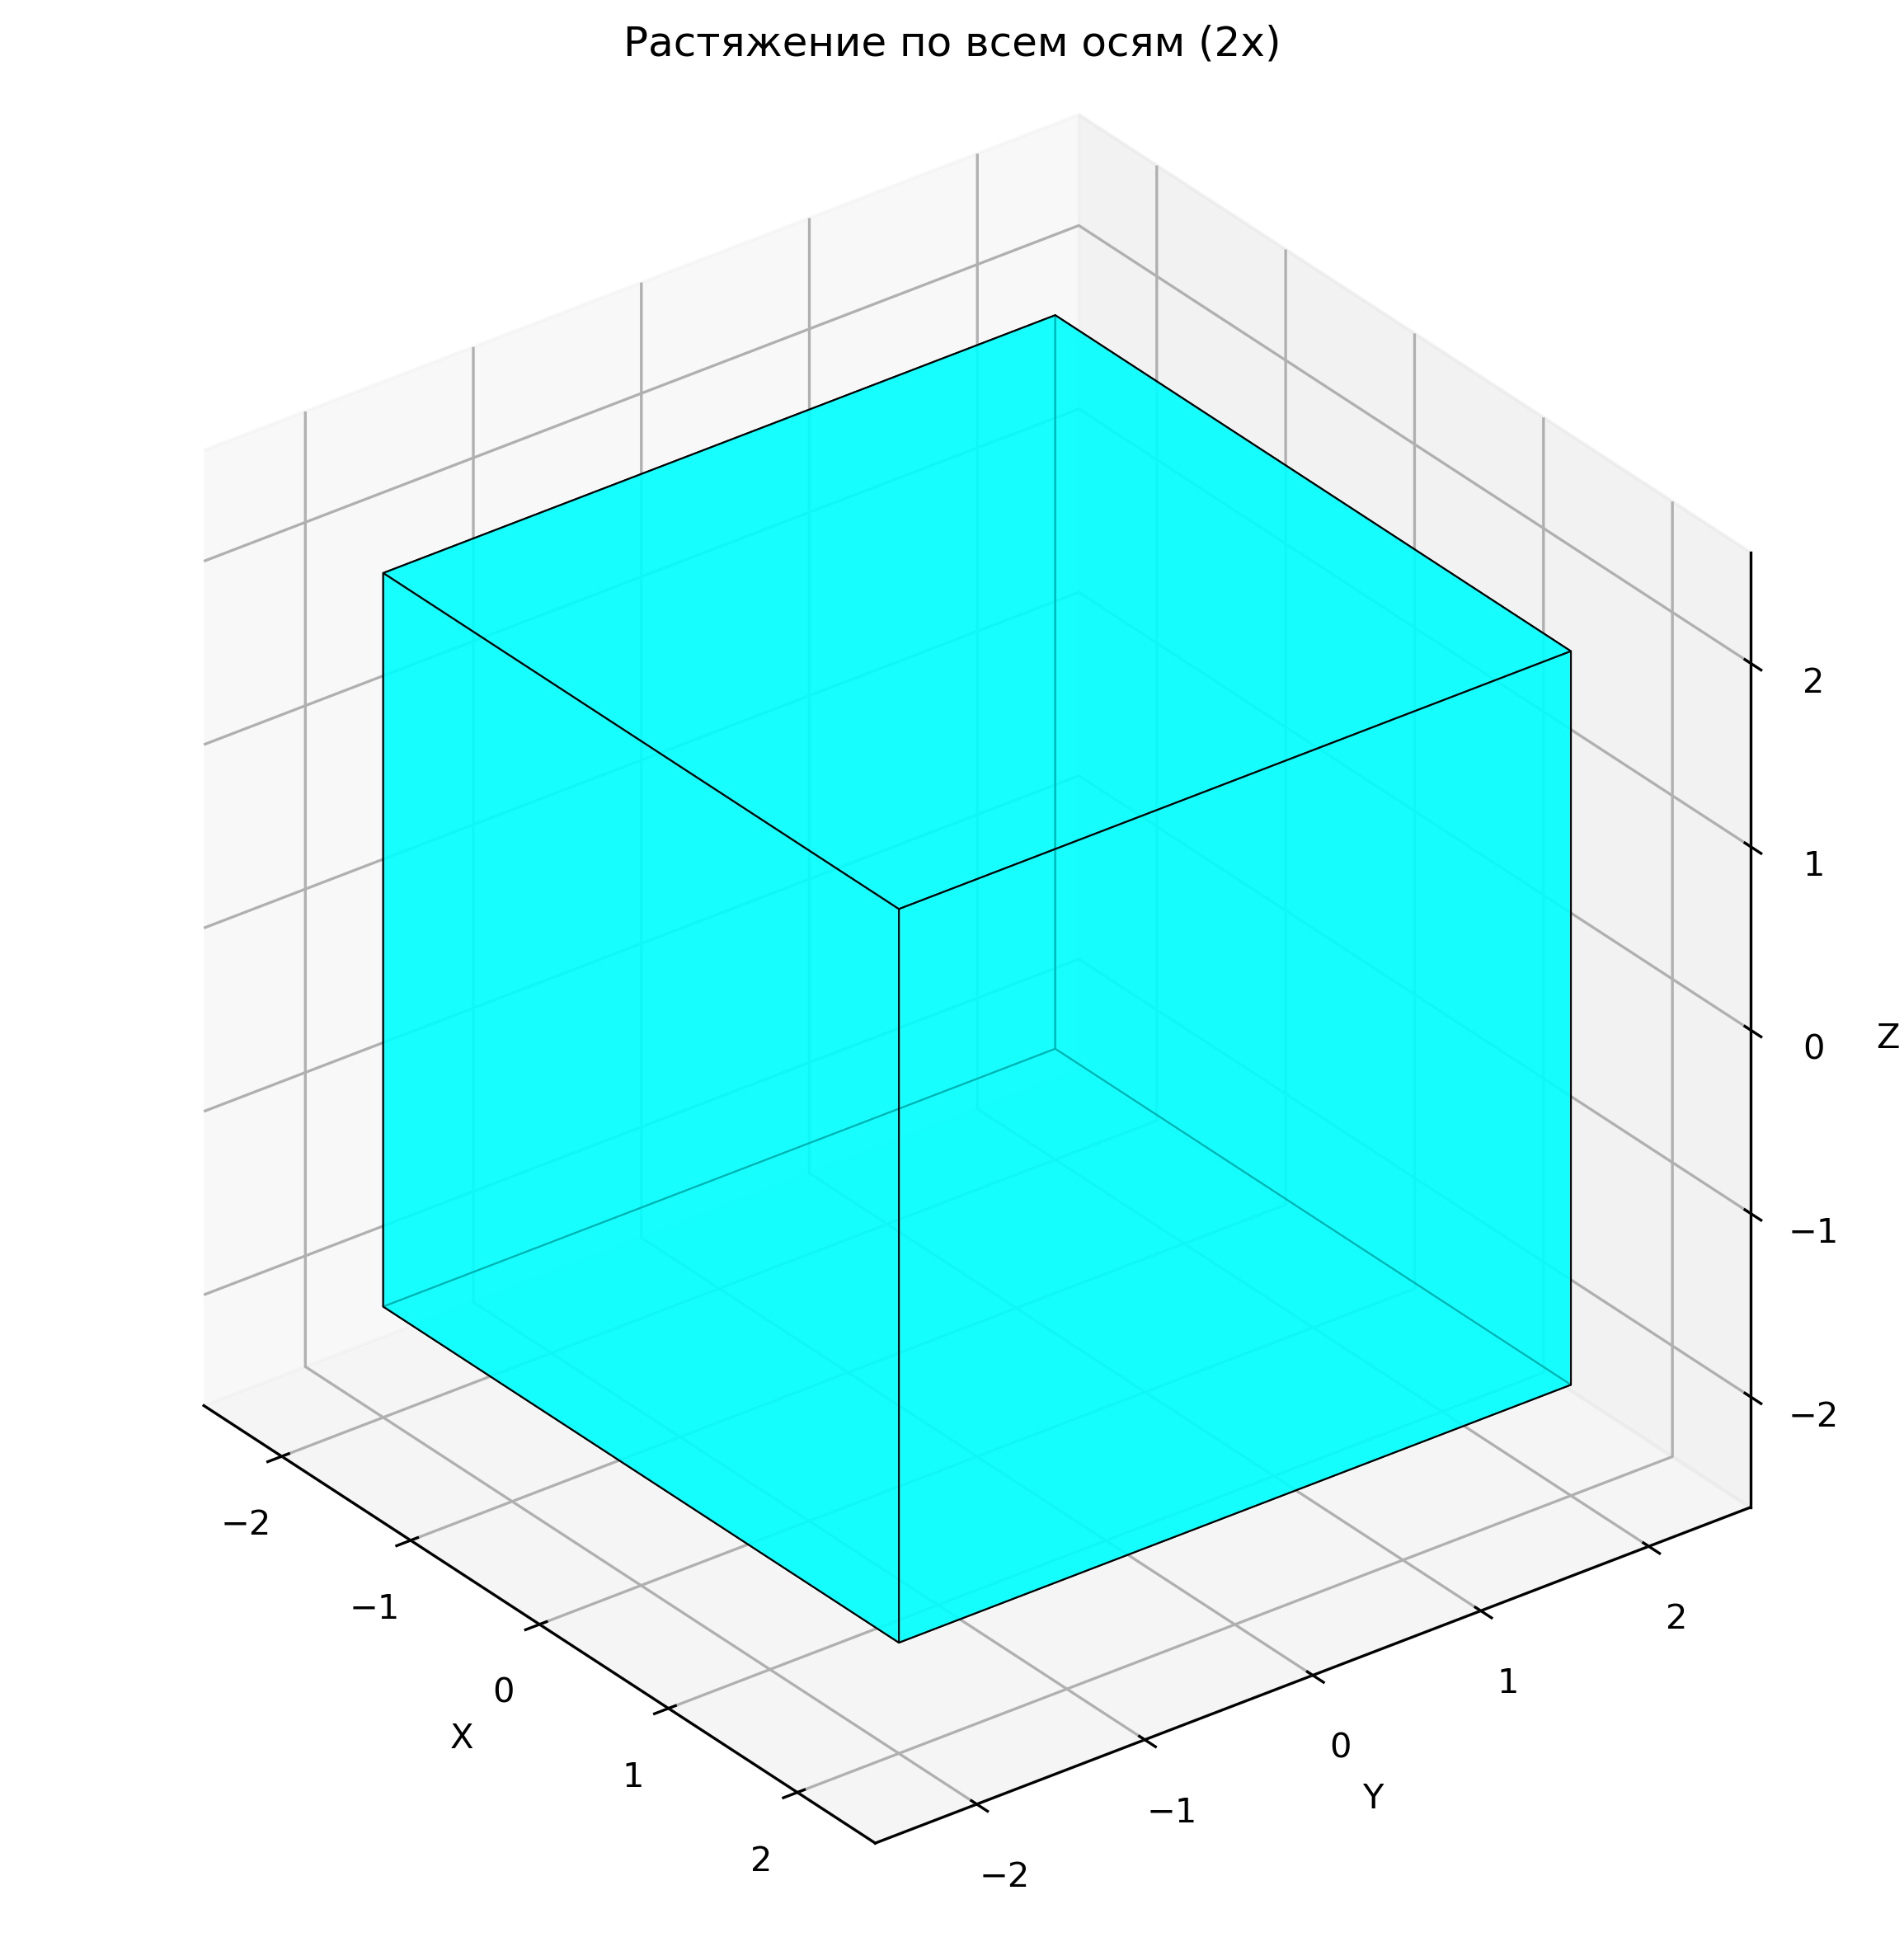
\includegraphics[width=0.8\textwidth]{images/task2/scale_all_large.png}
\caption{Растяжение по всем осям (2x)}
\end{figure}

\subsection*{Анализ}
\begin{itemize}
    \item Масштабирование по одной оси: кубик становится прямоугольным параллелепипедом
    \item Масштабирование по двум осям: кубик становится призмой
    \item Равномерное масштабирование: сохраняется форма, меняется размер
    \item Объем изменяется пропорционально произведению коэффициентов масштабирования
\end{itemize}

\section*{Задание 3: Перемещение кубика}

\subsection*{Постановка задачи}
Исследовать эффекты перемещения кубика и изучить композицию преобразований TS vs ST.

\subsection*{Математические основы}
Матрица перемещения в однородных координатах:
\begin{equation}
T = \begin{pmatrix}
1 & 0 & 0 & t_x \\
0 & 1 & 0 & t_y \\
0 & 0 & 1 & t_z \\
0 & 0 & 0 & 1
\end{pmatrix}
\end{equation}

где $t_x, t_y, t_z$ - компоненты вектора перемещения.

\subsection*{Результаты}
Исследованы различные случаи перемещения:

\begin{figure}[H]
\centering
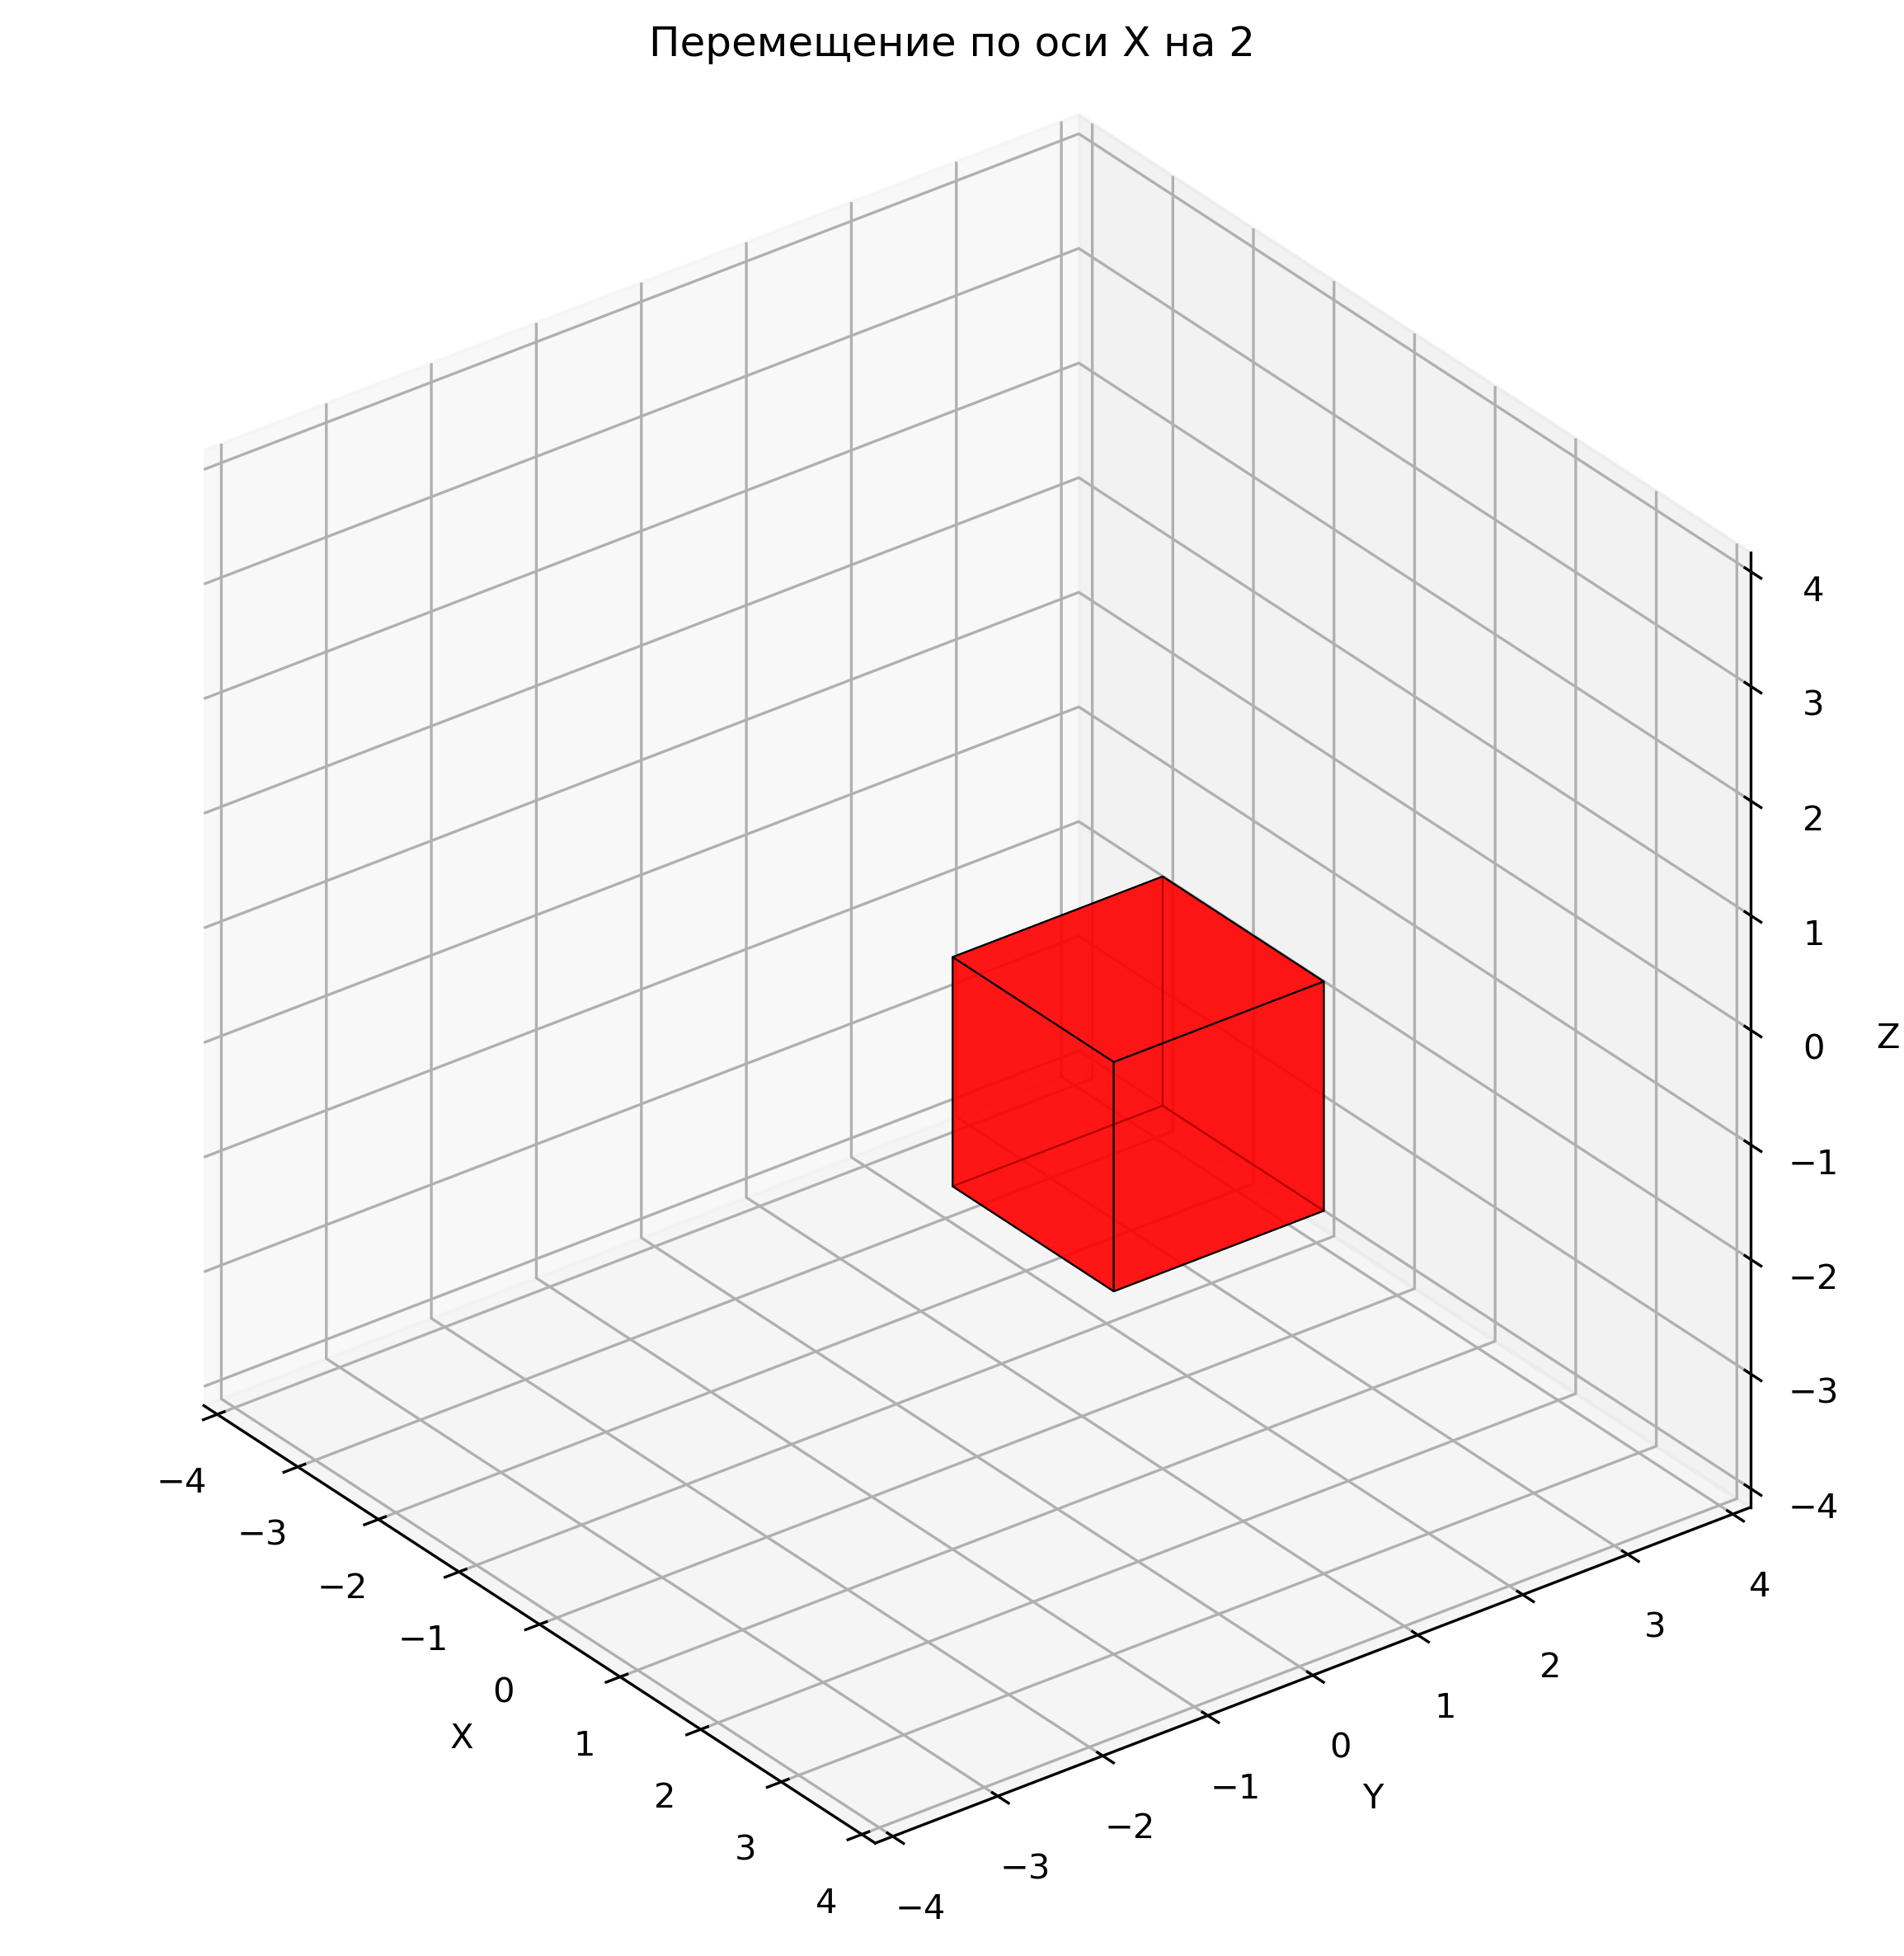
\includegraphics[width=0.8\textwidth]{images/task3/translate_x.png}
\caption{Перемещение по оси X на 2}
\end{figure}

\begin{figure}[H]
\centering
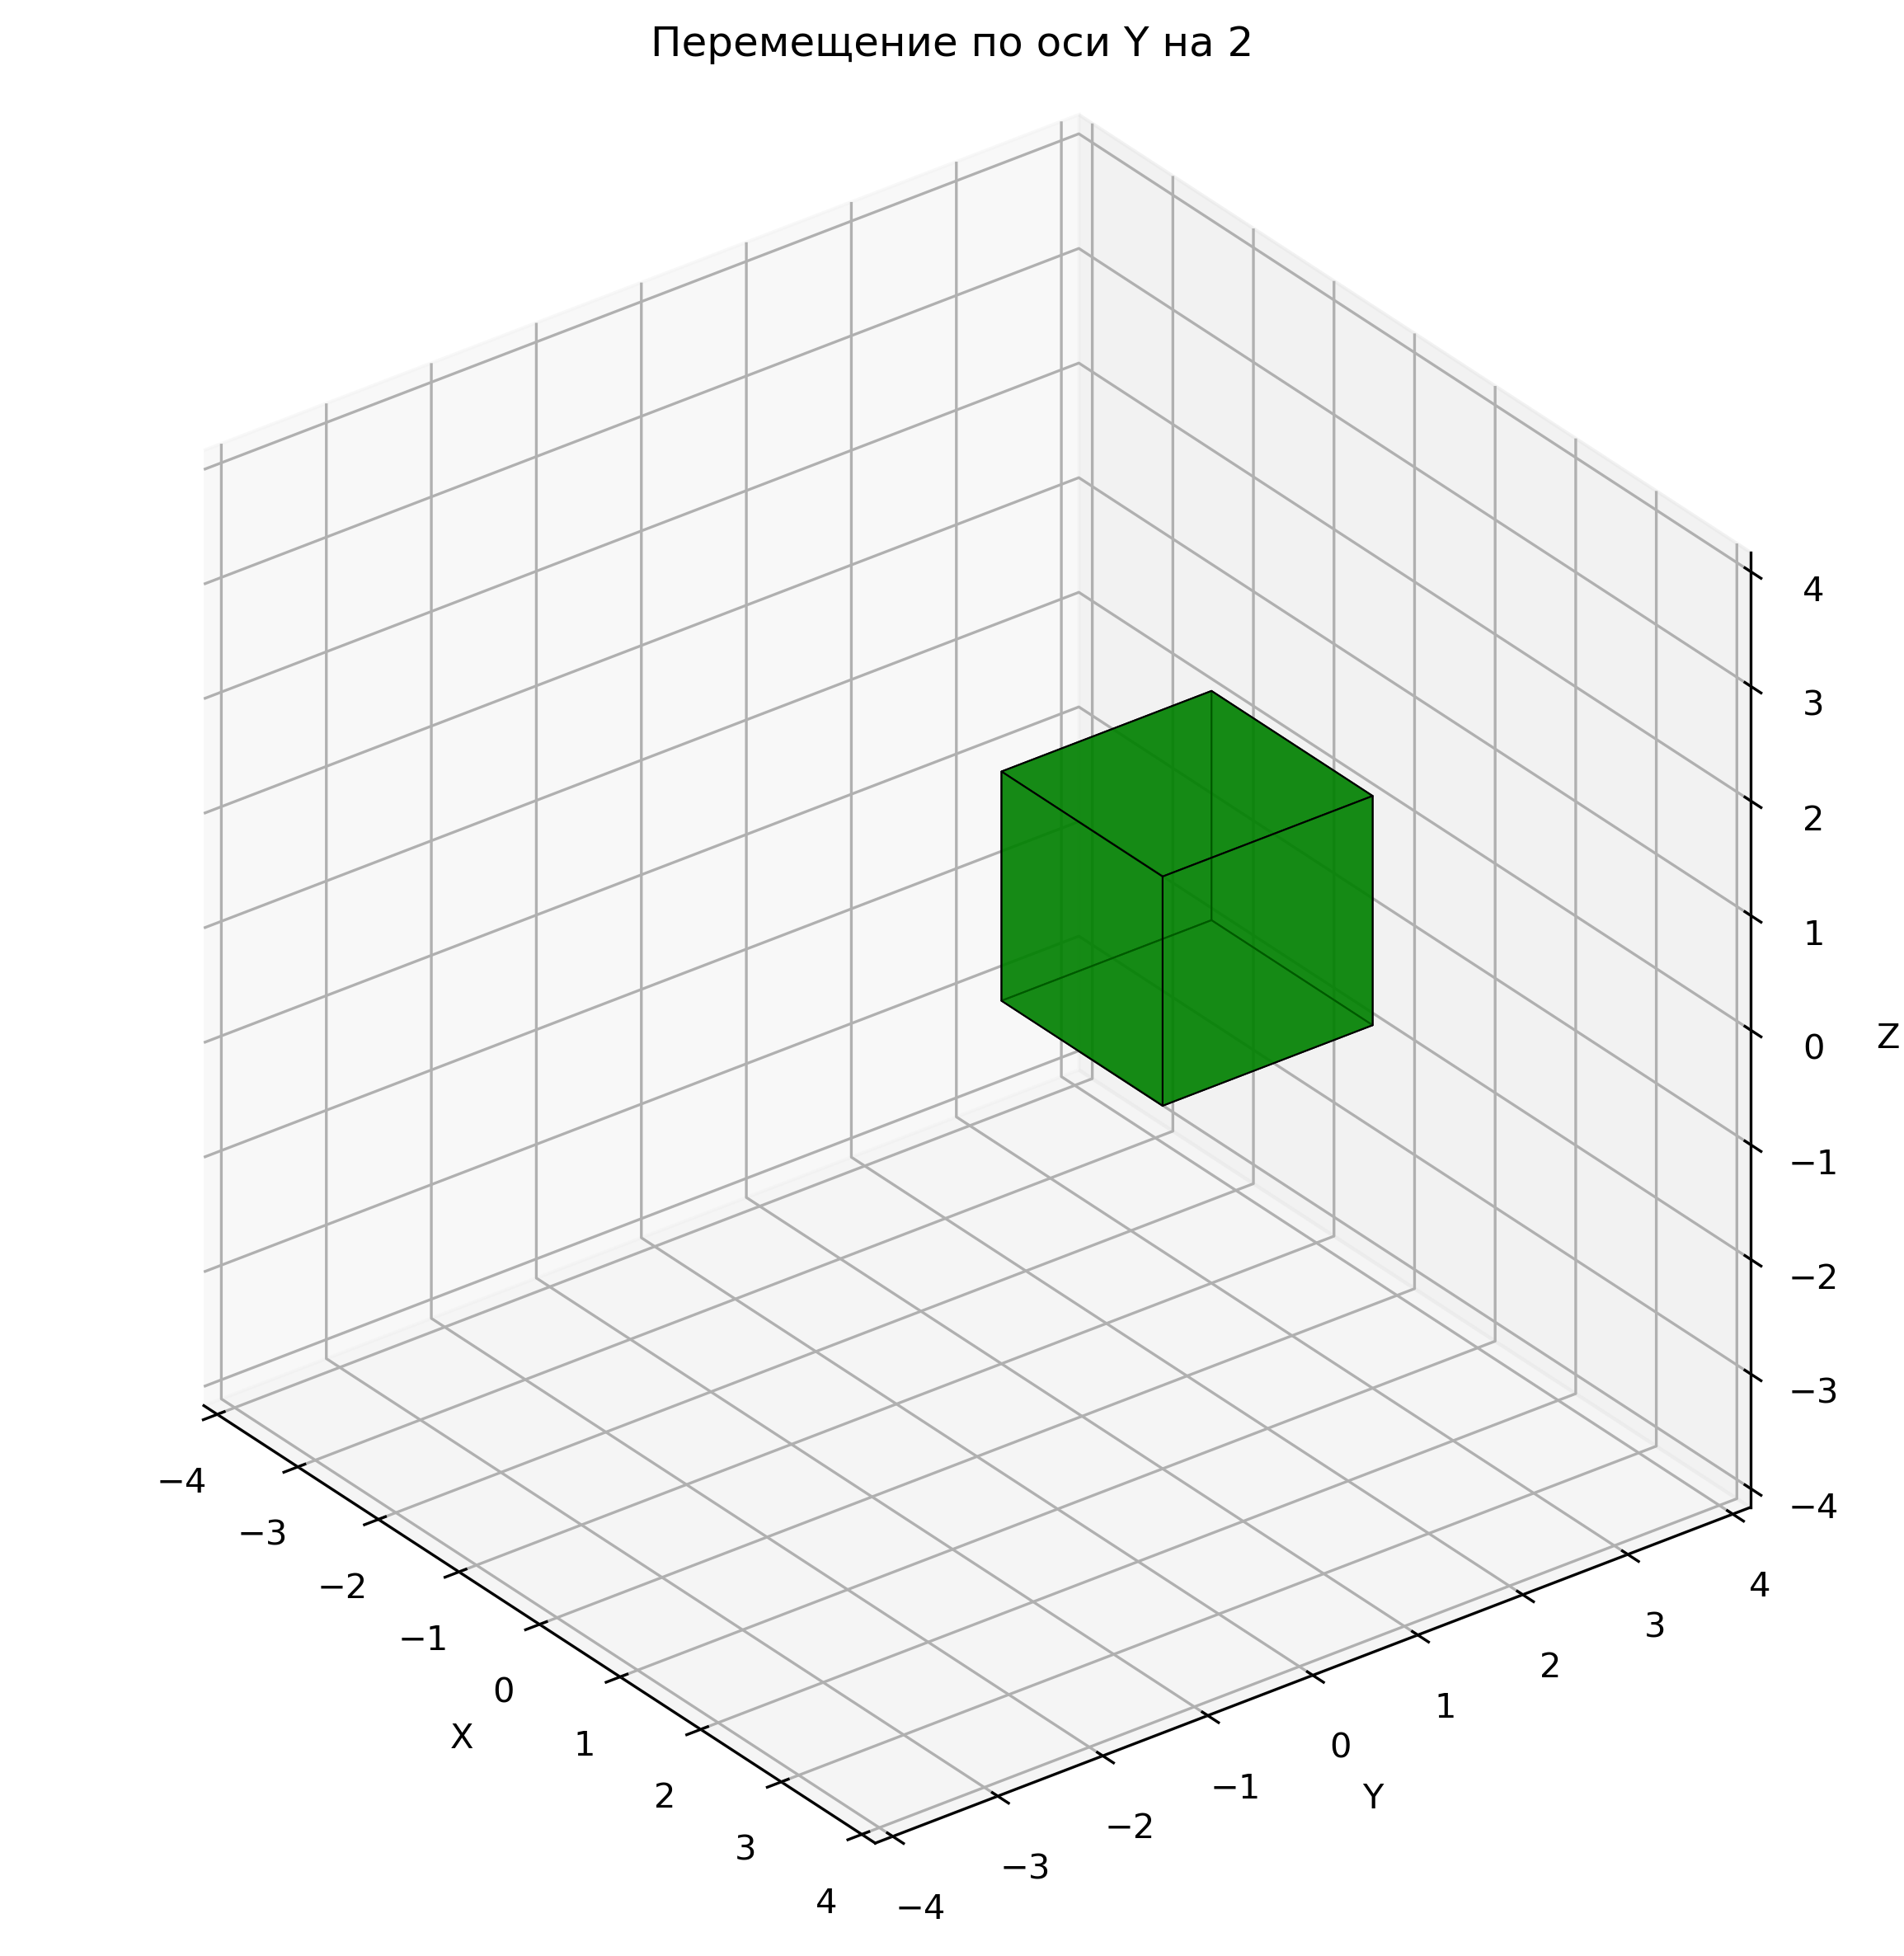
\includegraphics[width=0.8\textwidth]{images/task3/translate_y.png}
\caption{Перемещение по оси Y на 2}
\end{figure}

\begin{figure}[H]
\centering
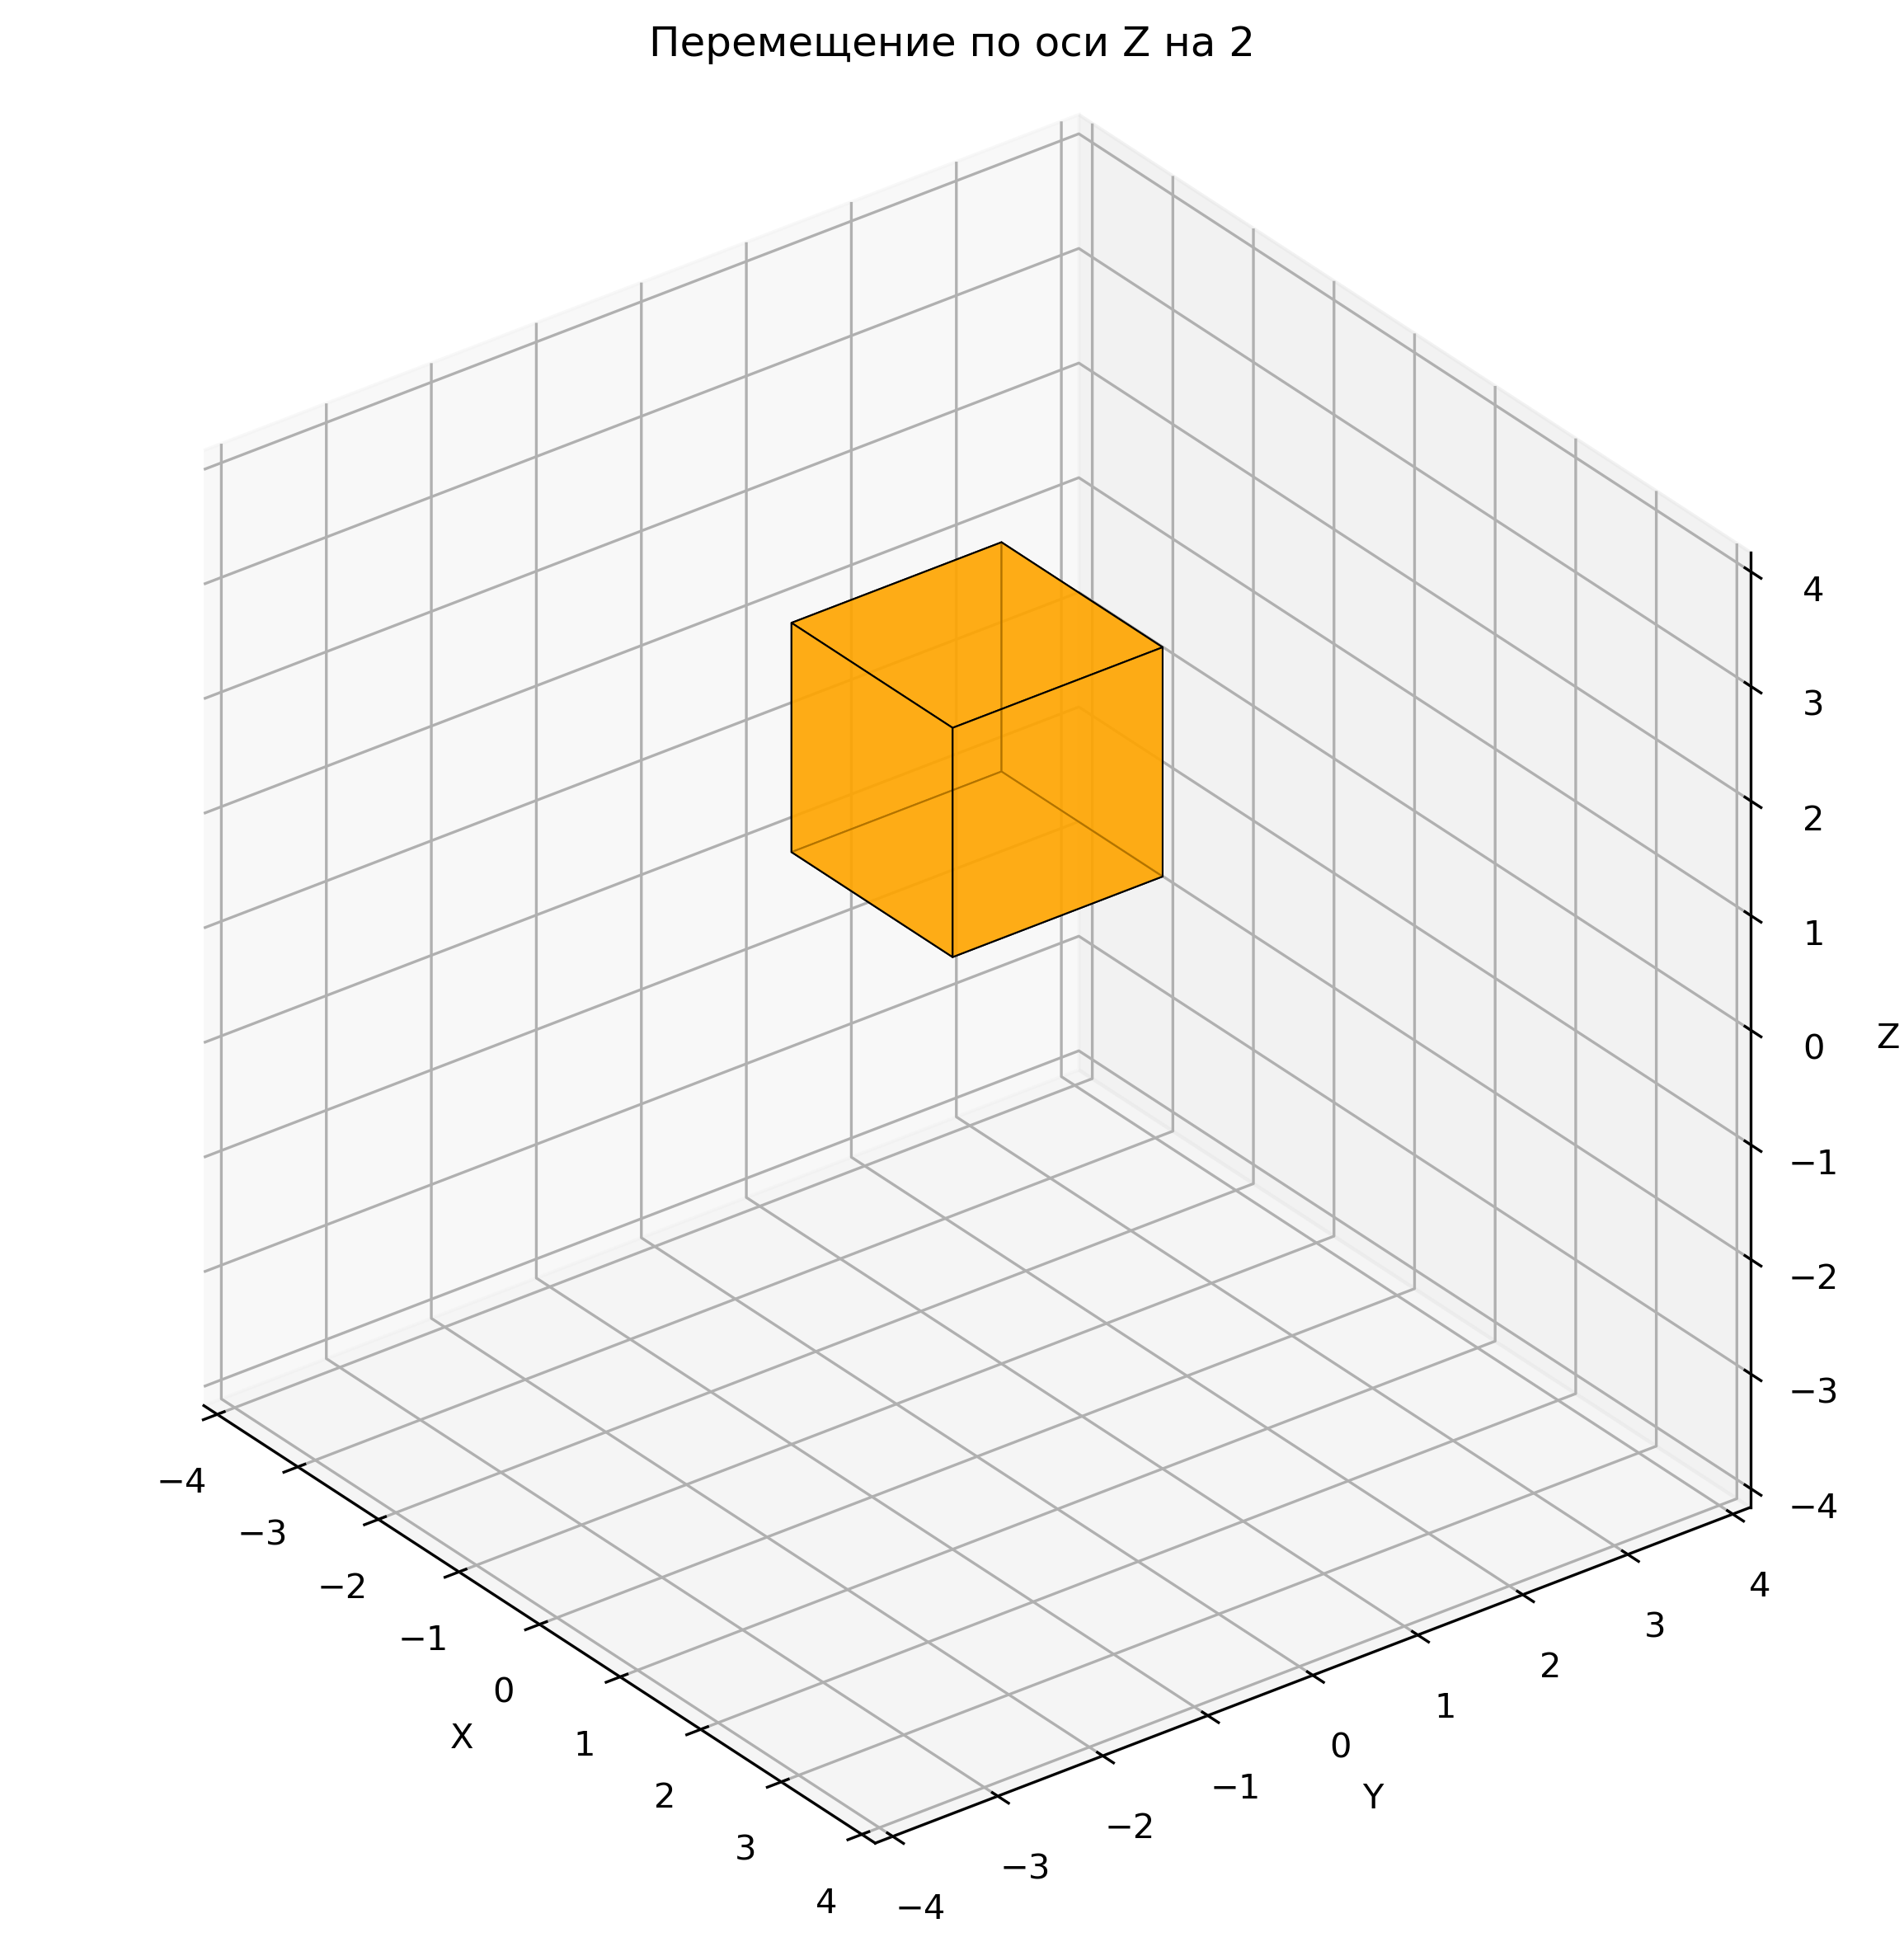
\includegraphics[width=0.8\textwidth]{images/task3/translate_z.png}
\caption{Перемещение по оси Z на 2}
\end{figure}

\begin{figure}[H]
\centering
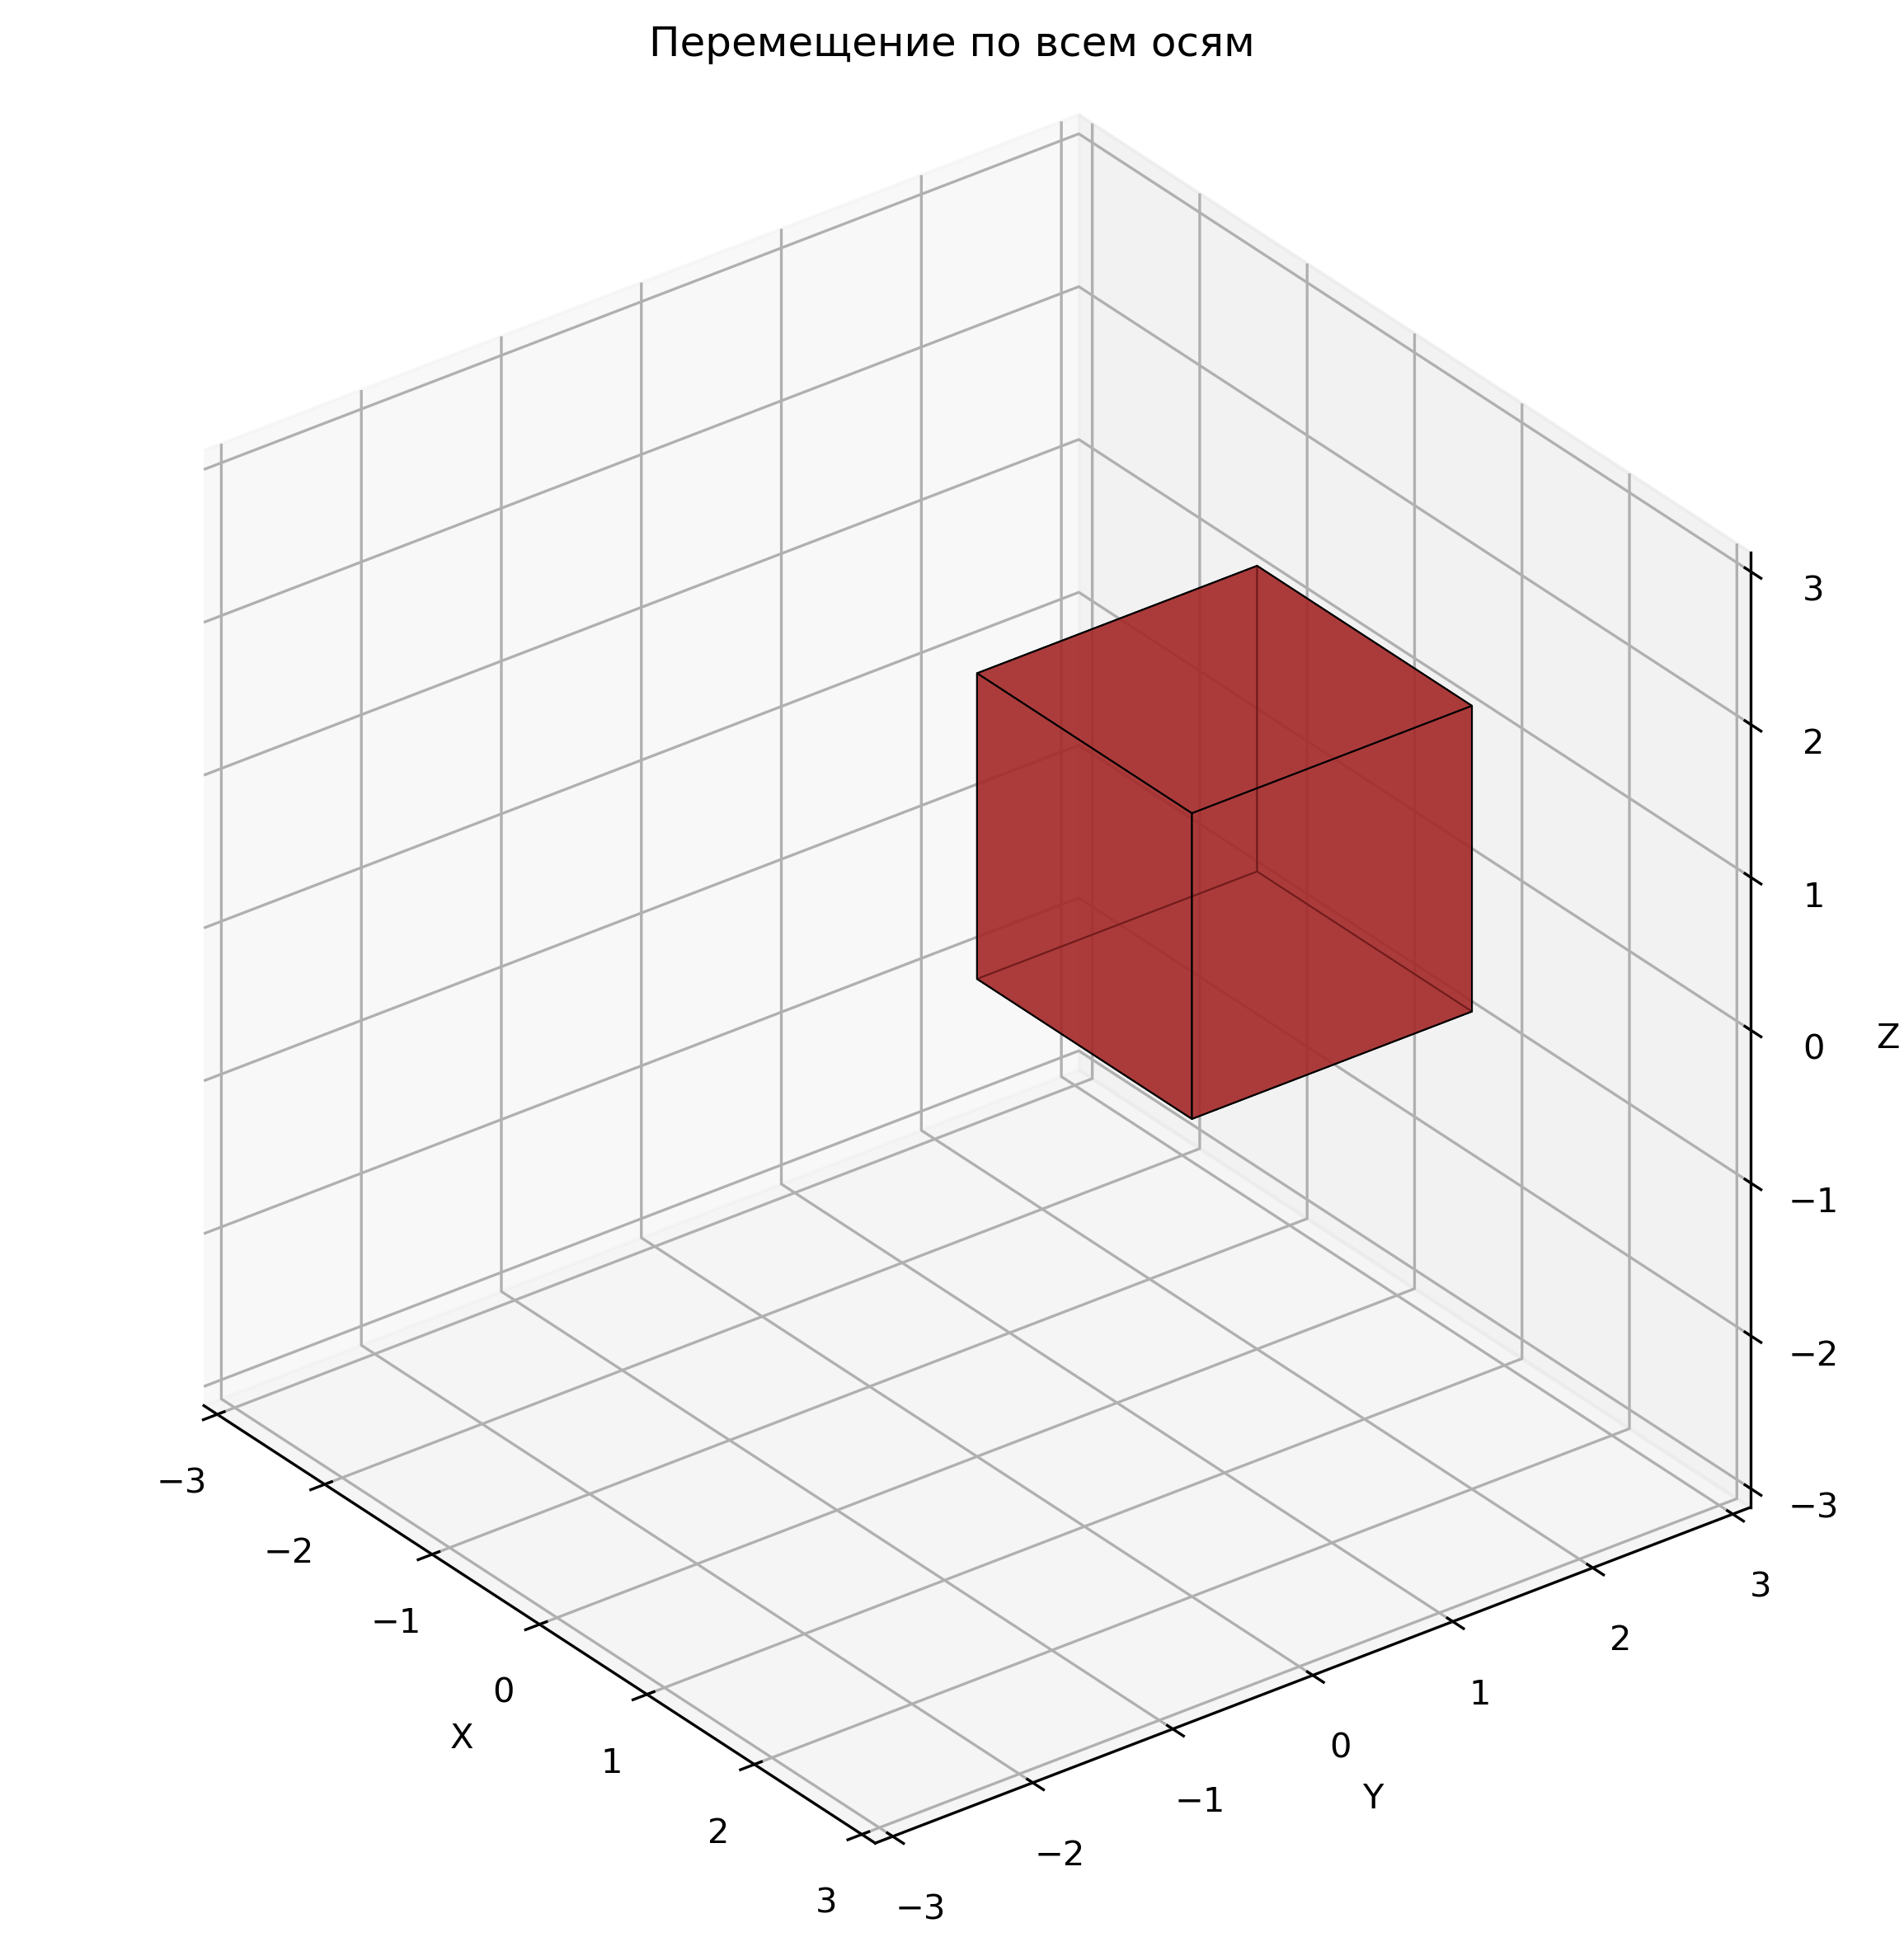
\includegraphics[width=0.8\textwidth]{images/task3/translate_xyz.png}
\caption{Перемещение по всем осям}
\end{figure}

\subsection*{Исследование композиции TS vs ST}

\begin{figure}[H]
\centering
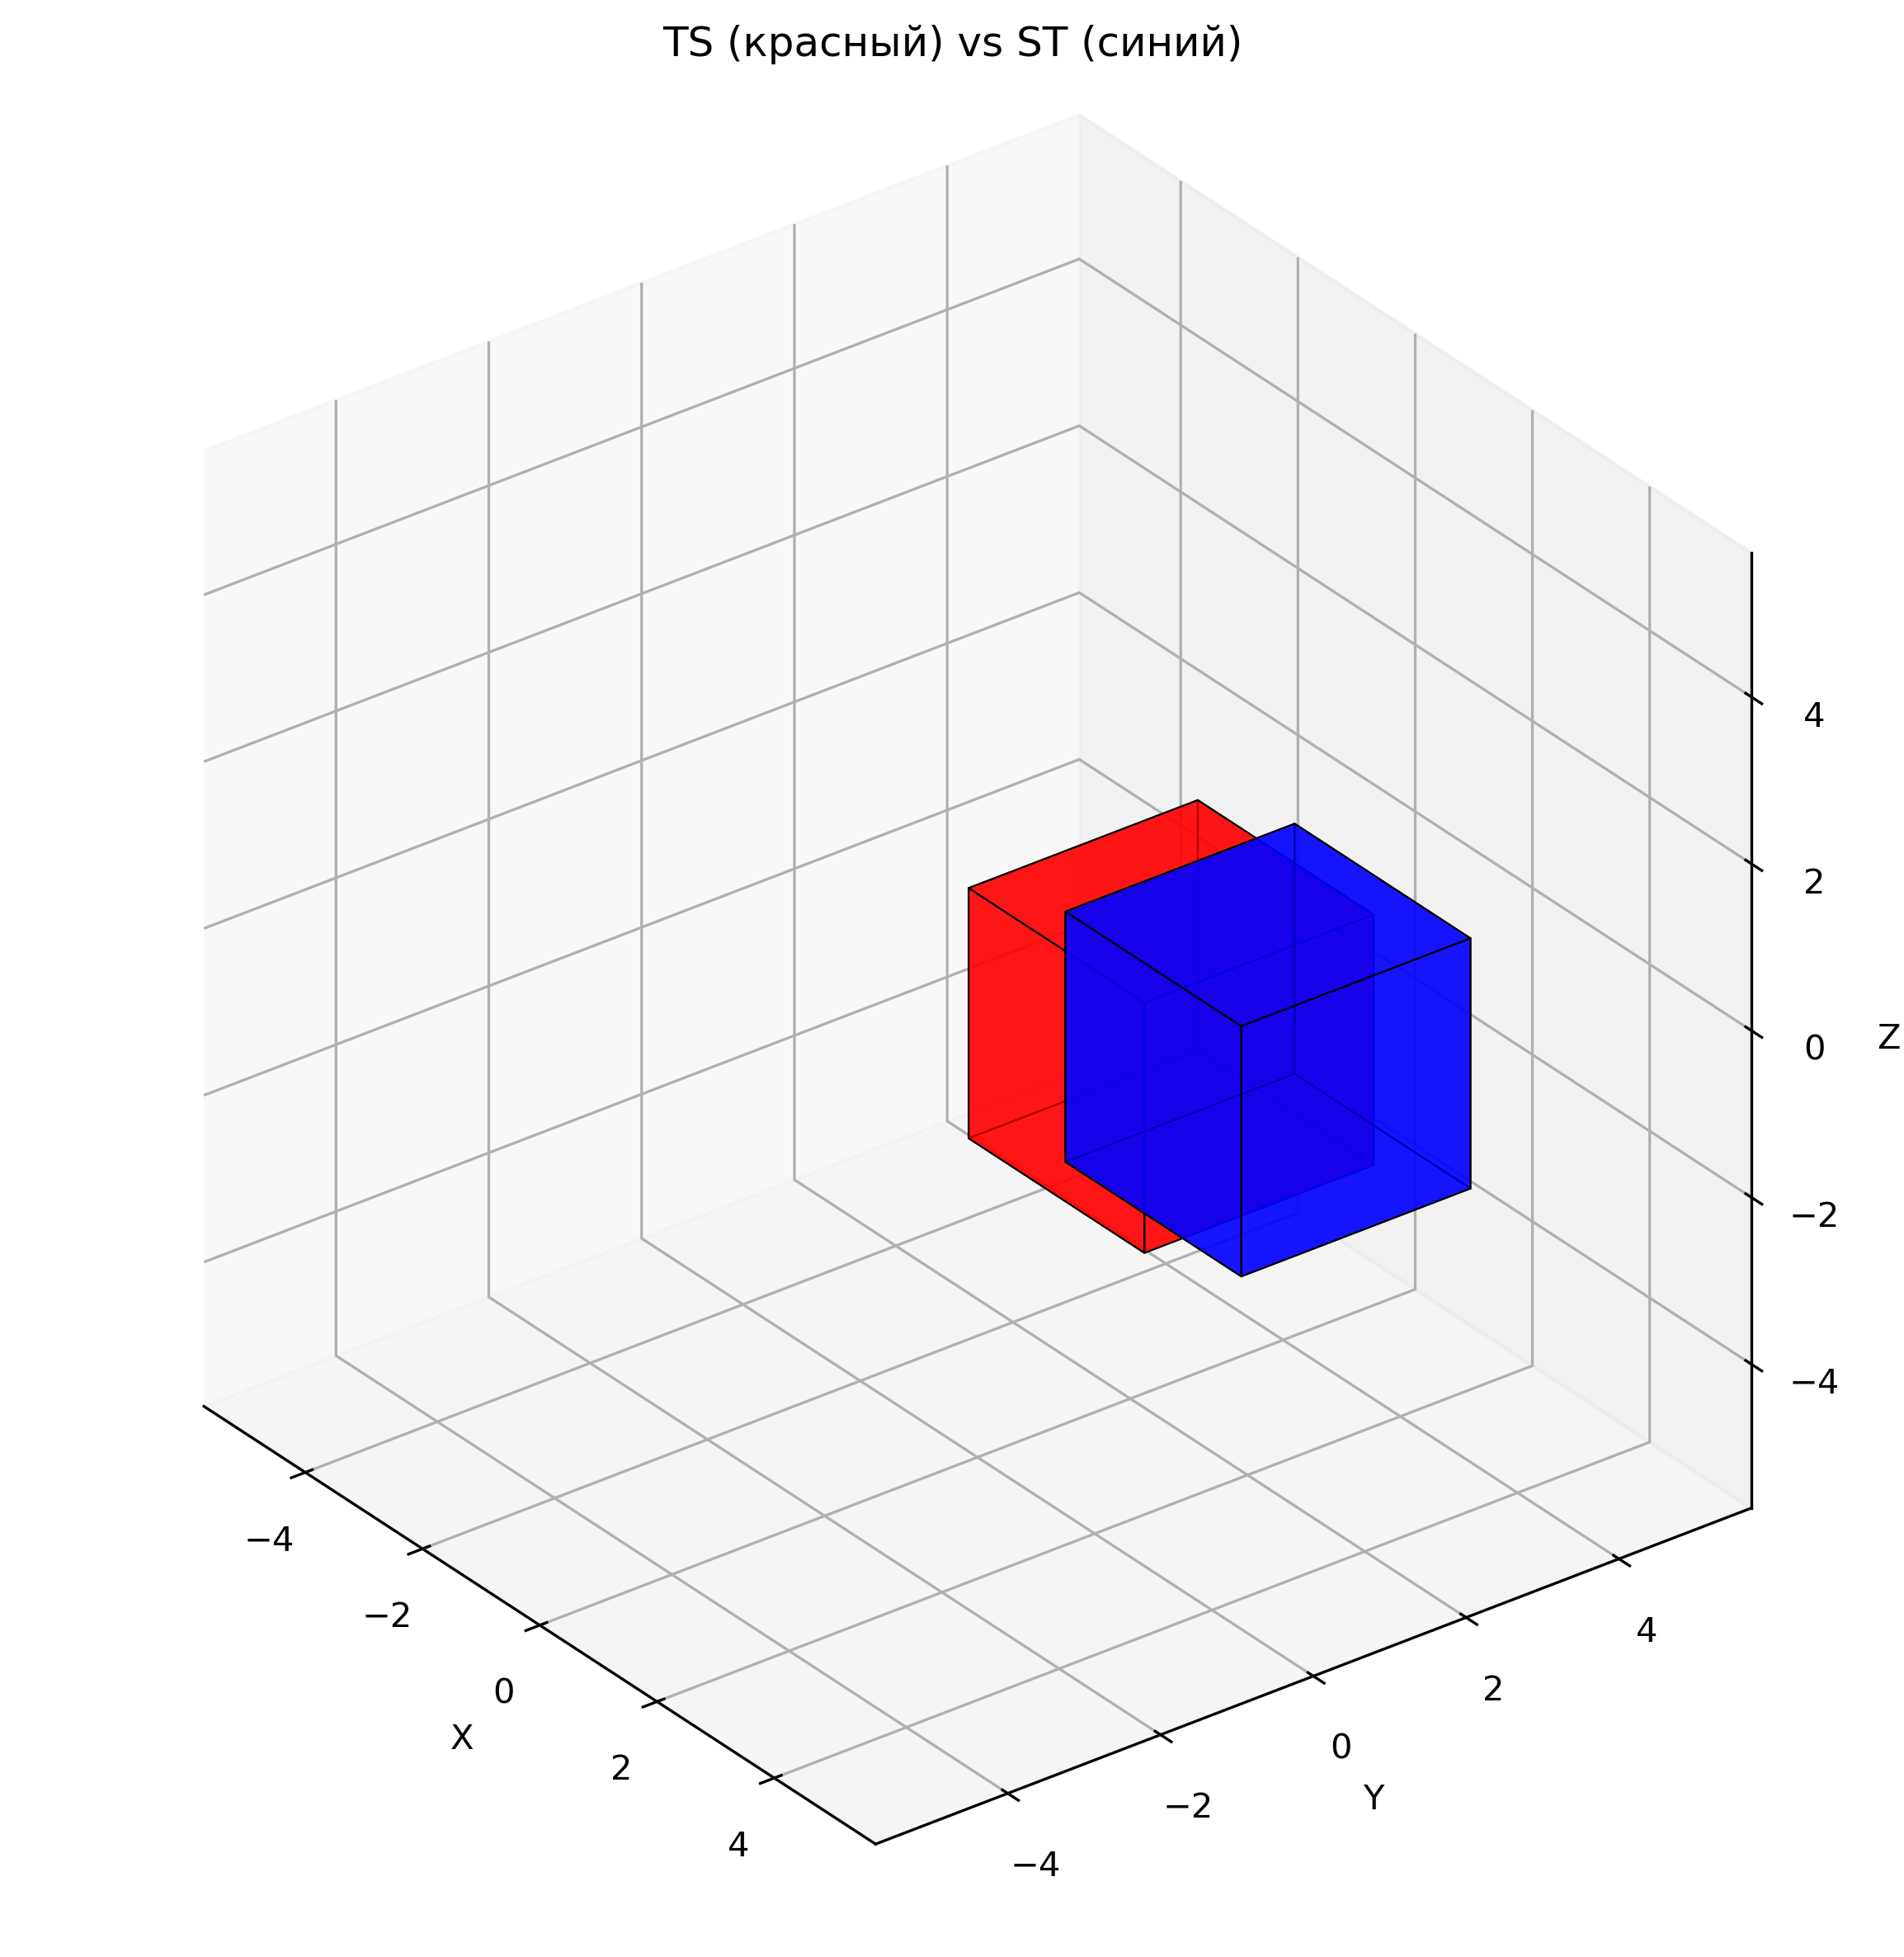
\includegraphics[width=0.8\textwidth]{images/task3/ts_vs_st.png}
\caption{Сравнение TS (красный) vs ST (синий)}
\end{figure}

\subsection*{Анализ различий}
\begin{itemize}
    \item При TS: сначала масштабирование (изменение размера), потом перемещение
    \item При ST: сначала перемещение, потом масштабирование (включая перемещение)
    \item Масштабирование влияет на все координаты, включая перемещение
    \item TS $\neq$ ST: преобразования не коммутируют
\end{itemize}

\section*{Задание 4: Вращение кубика}

\subsection*{Постановка задачи}
Реализовать вращение кубика вокруг произвольной оси и исследовать теорему вращения Эйлера.

\subsection*{Математические основы}
Матрица вращения вокруг вектора $\mathbf{v}$ на угол $\theta$:
\begin{equation}
R = e^{J\theta}
\end{equation}

где $J$ - кососимметричная матрица:
\begin{equation}
J = \begin{pmatrix}
0 & -v_z & v_y & 0 \\
v_z & 0 & -v_x & 0 \\
-v_y & v_x & 0 & 0 \\
0 & 0 & 0 & 0
\end{pmatrix}
\end{equation}

\subsection*{Результаты}
Исследованы вращения вокруг различных осей:

\begin{figure}[H]
\centering
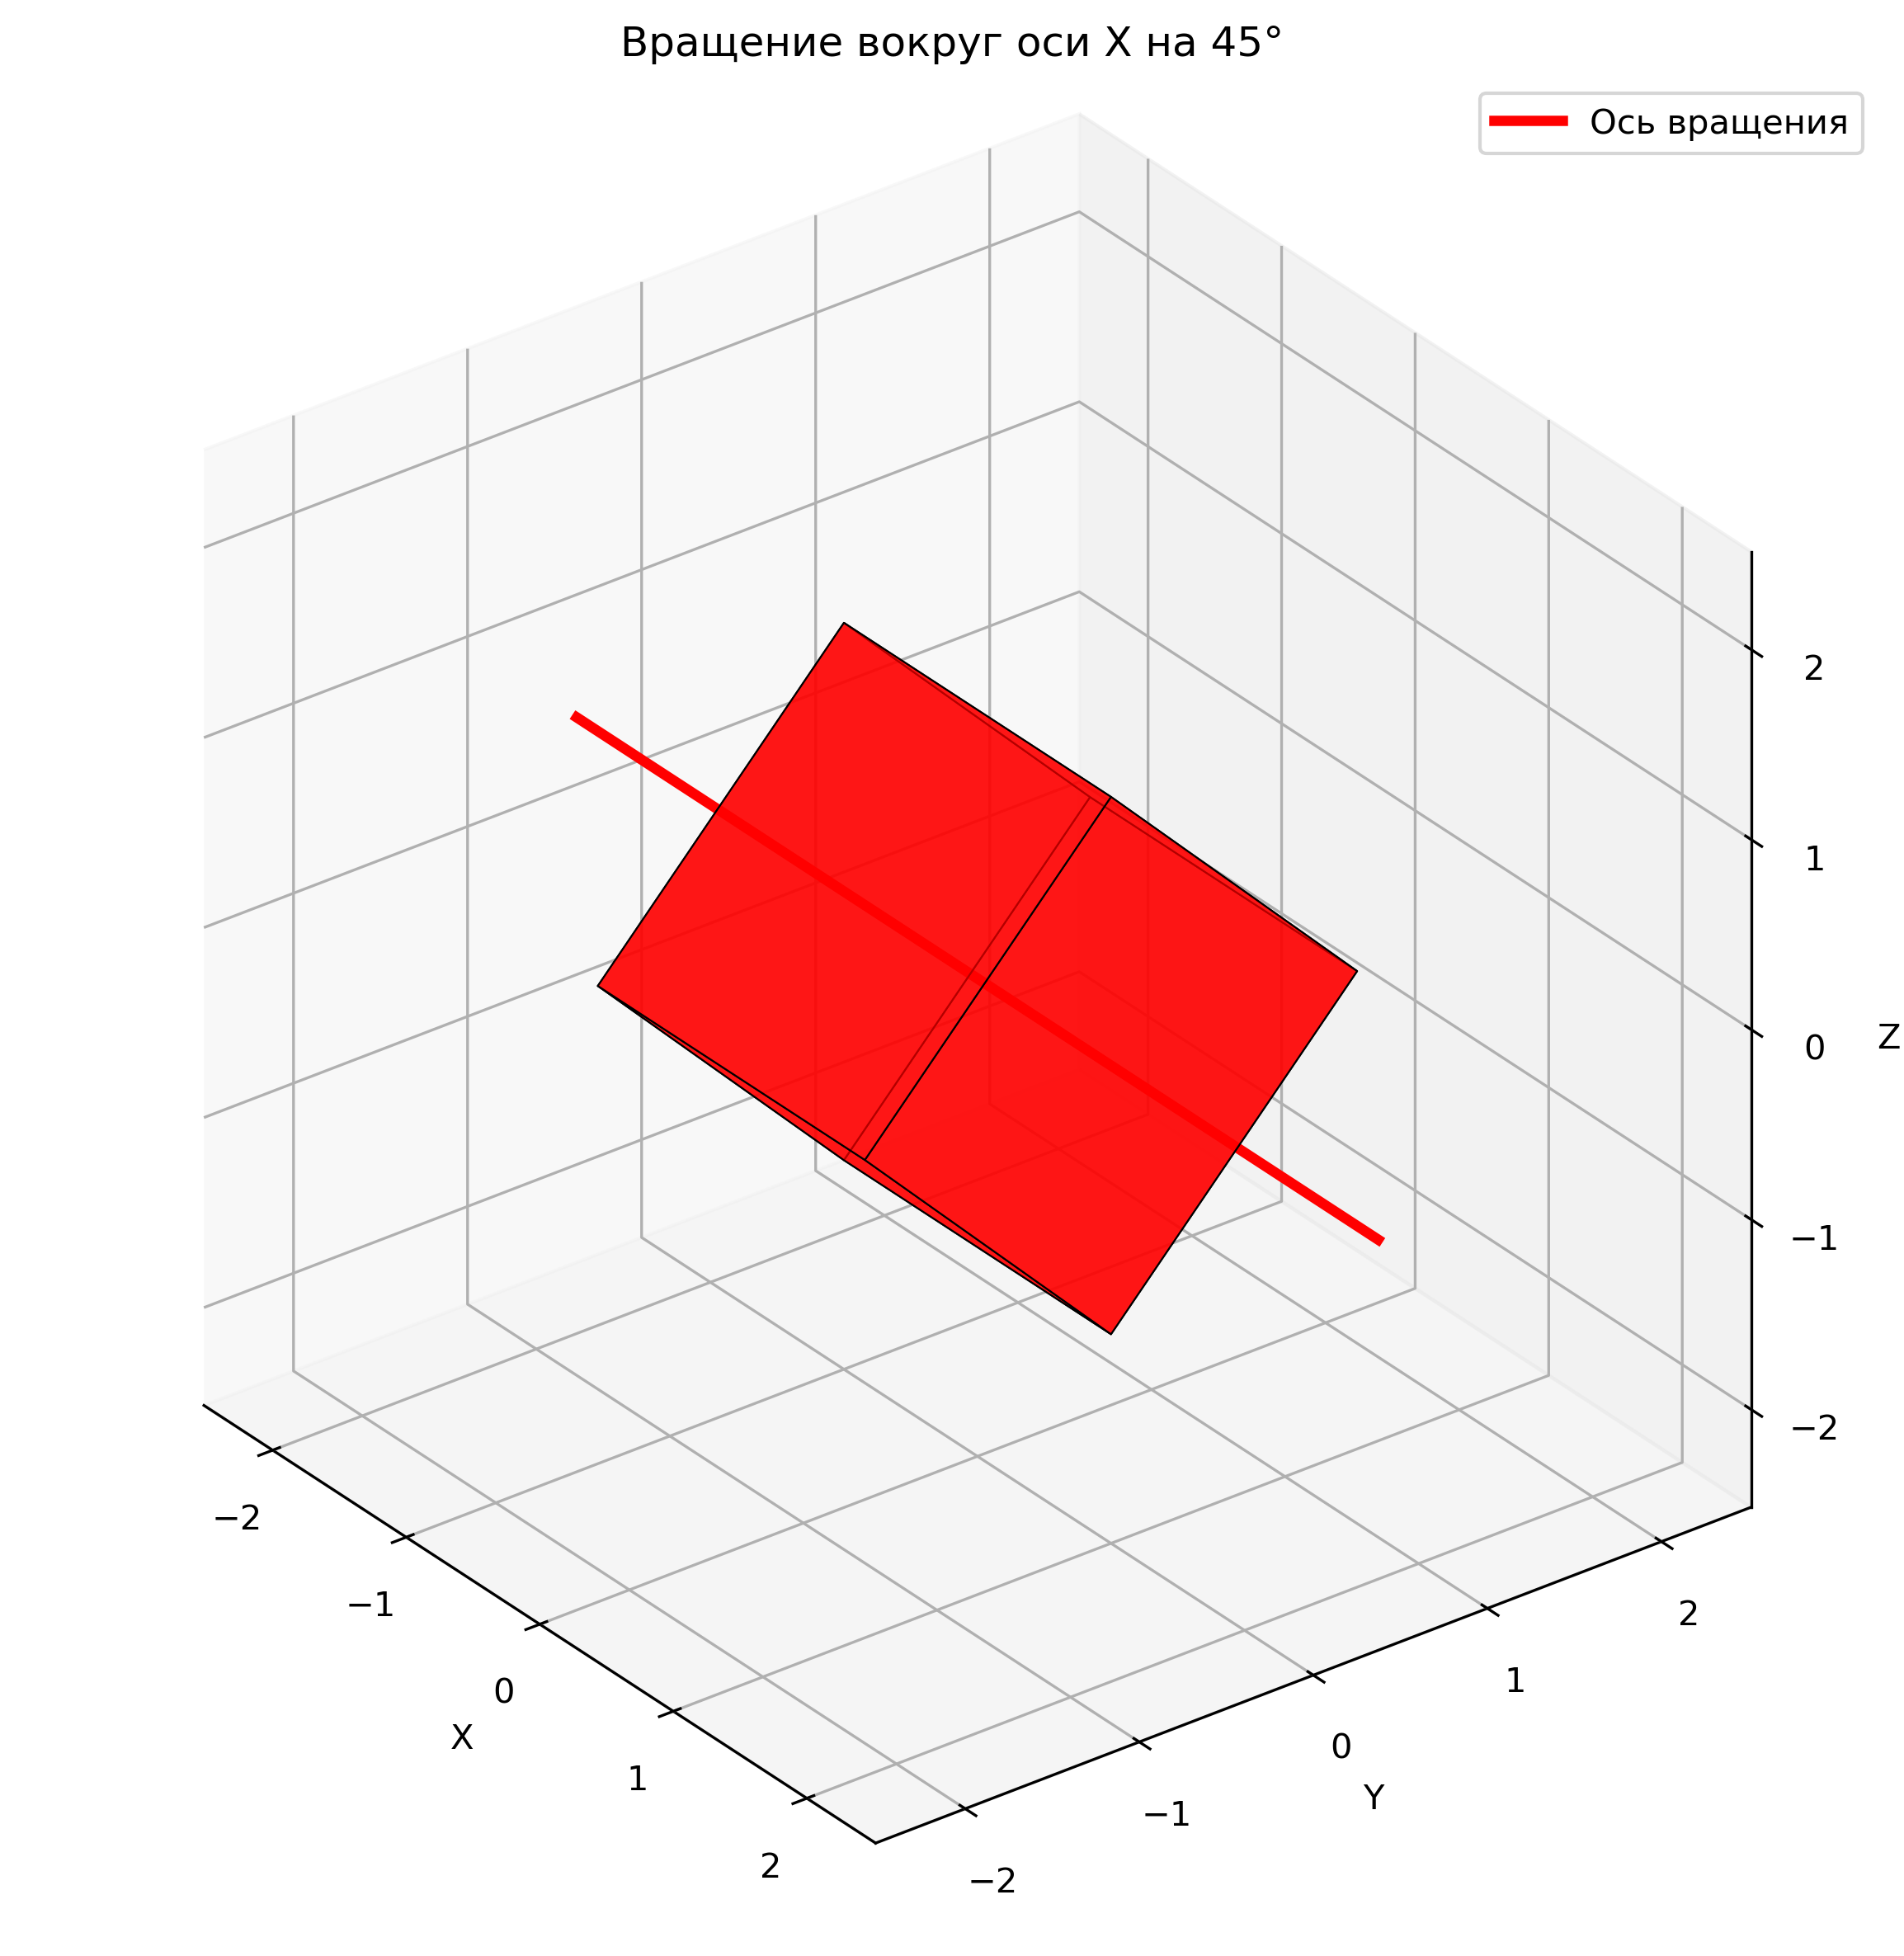
\includegraphics[width=0.8\textwidth]{images/task4/rotate_x.png}
\caption{Вращение вокруг оси X на 45°}
\end{figure}

\begin{figure}[H]
\centering
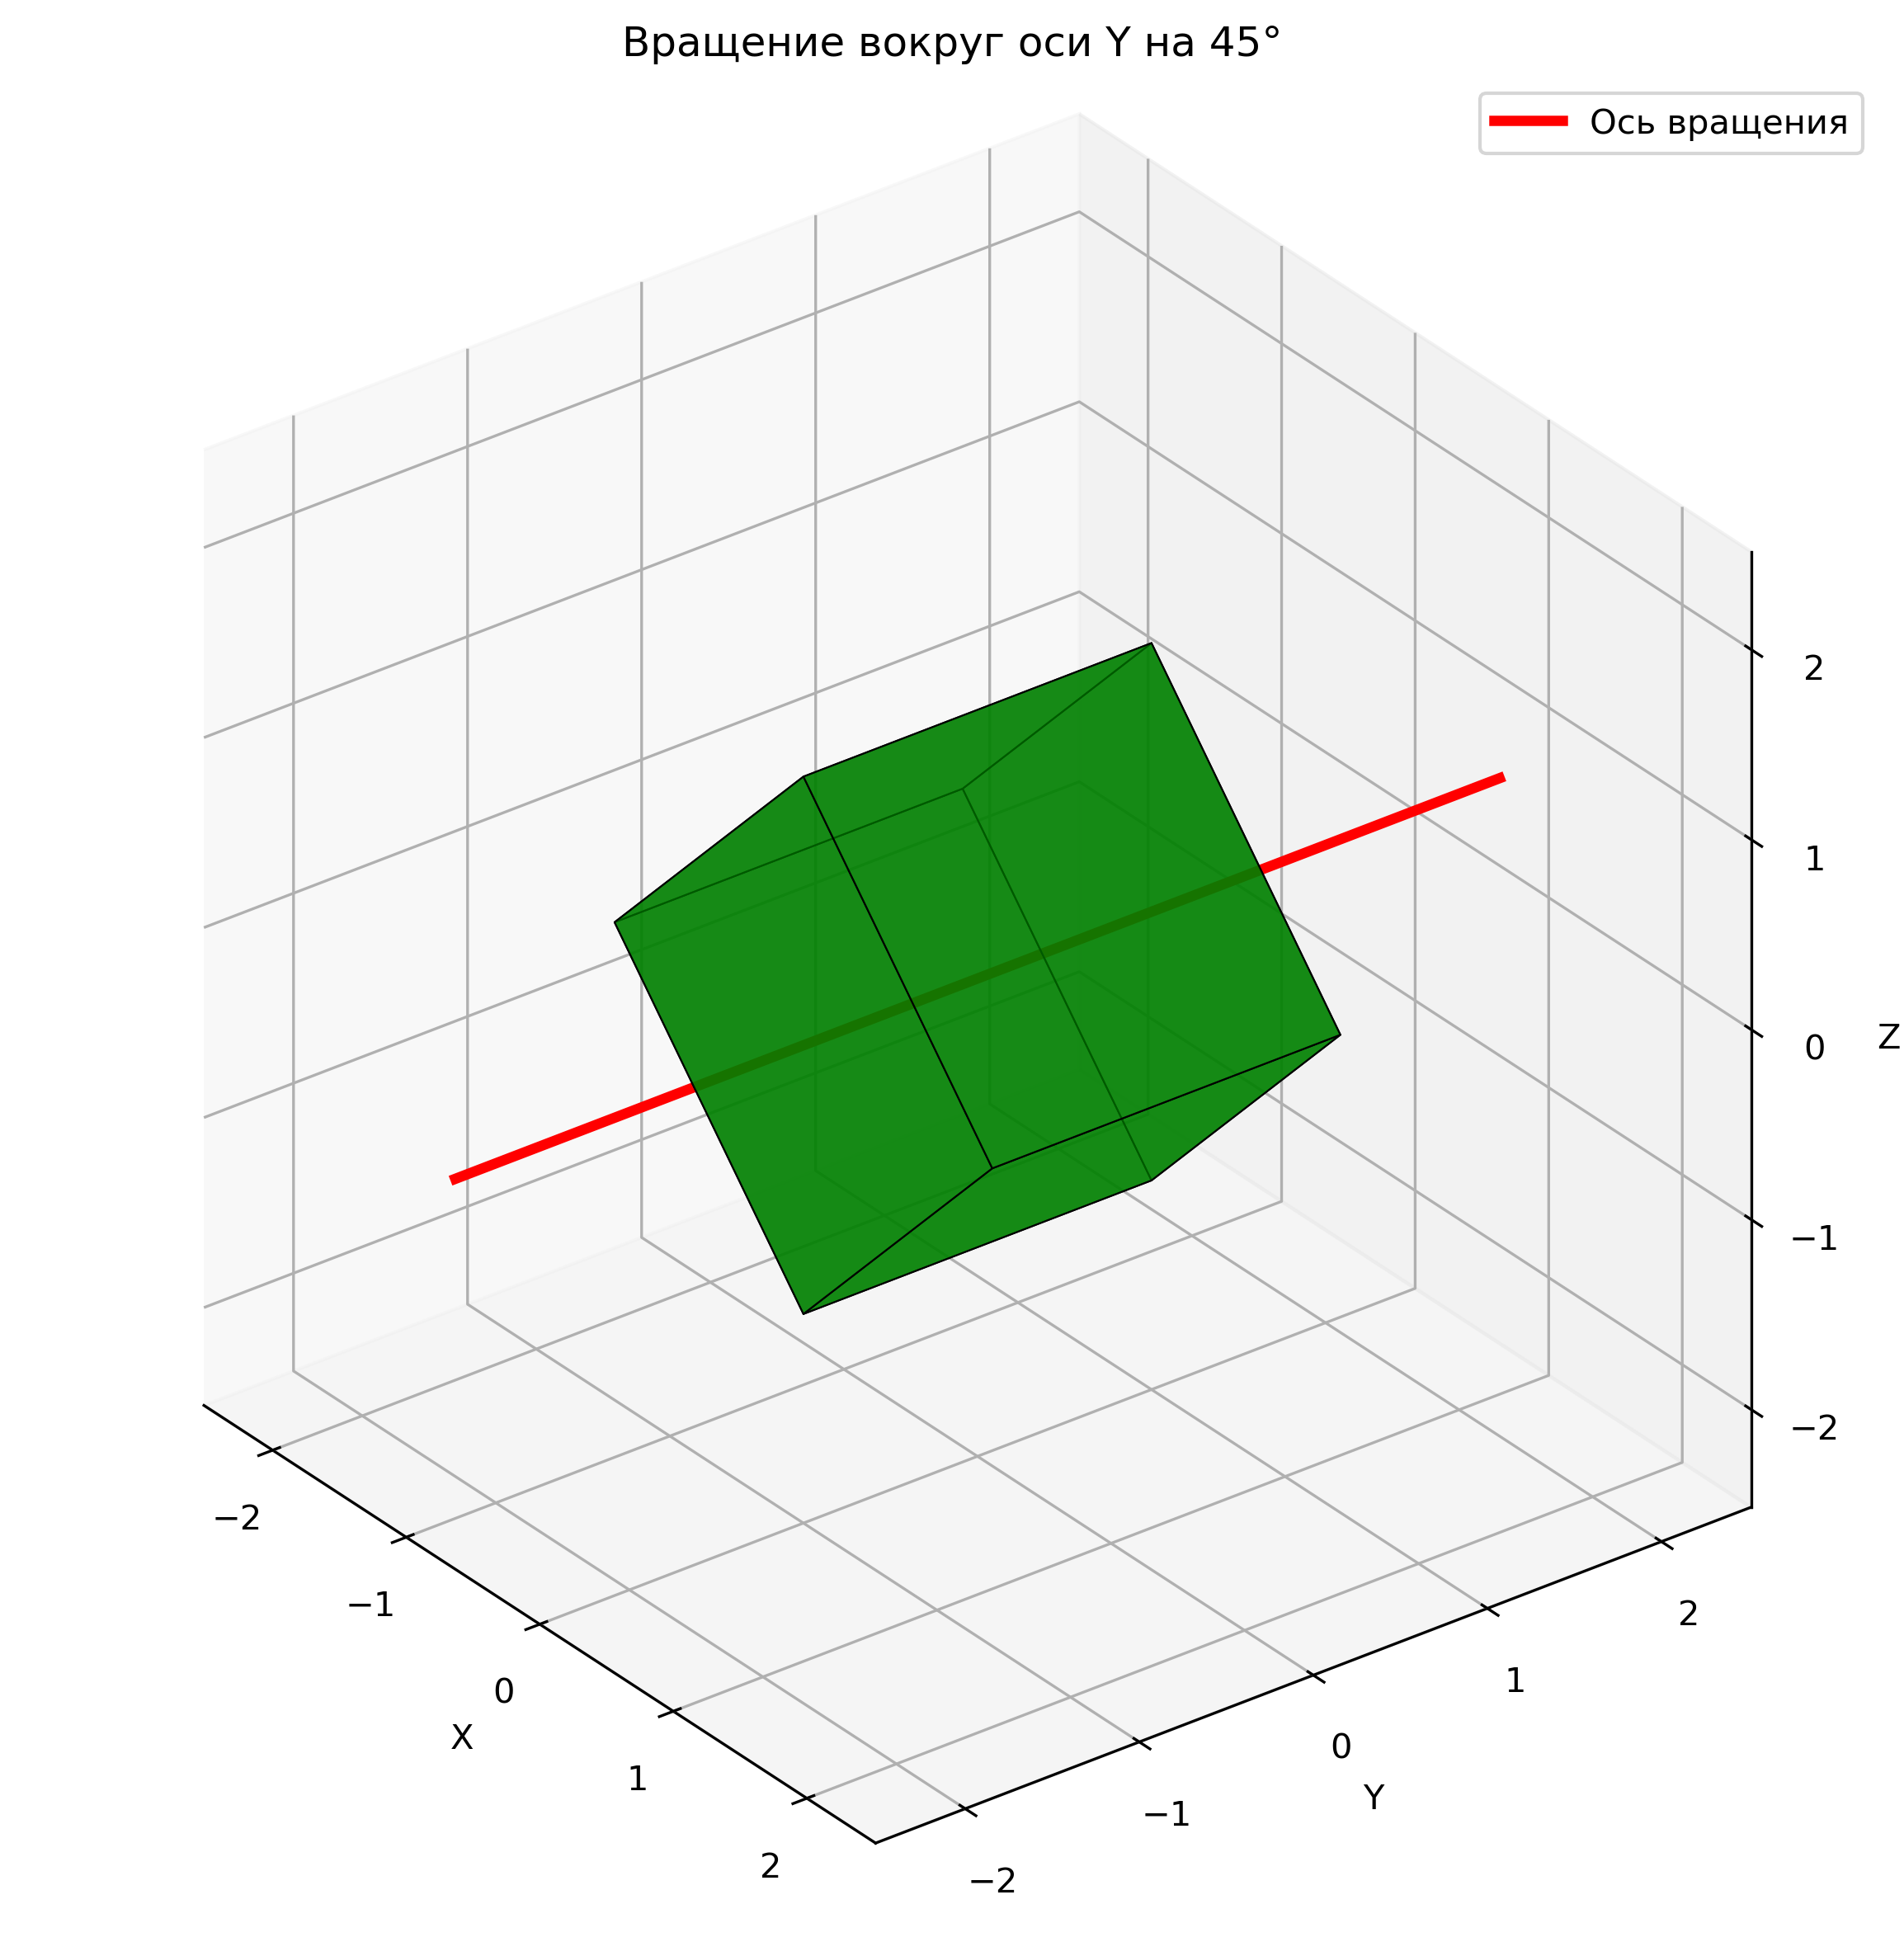
\includegraphics[width=0.8\textwidth]{images/task4/rotate_y.png}
\caption{Вращение вокруг оси Y на 45°}
\end{figure}

\begin{figure}[H]
\centering
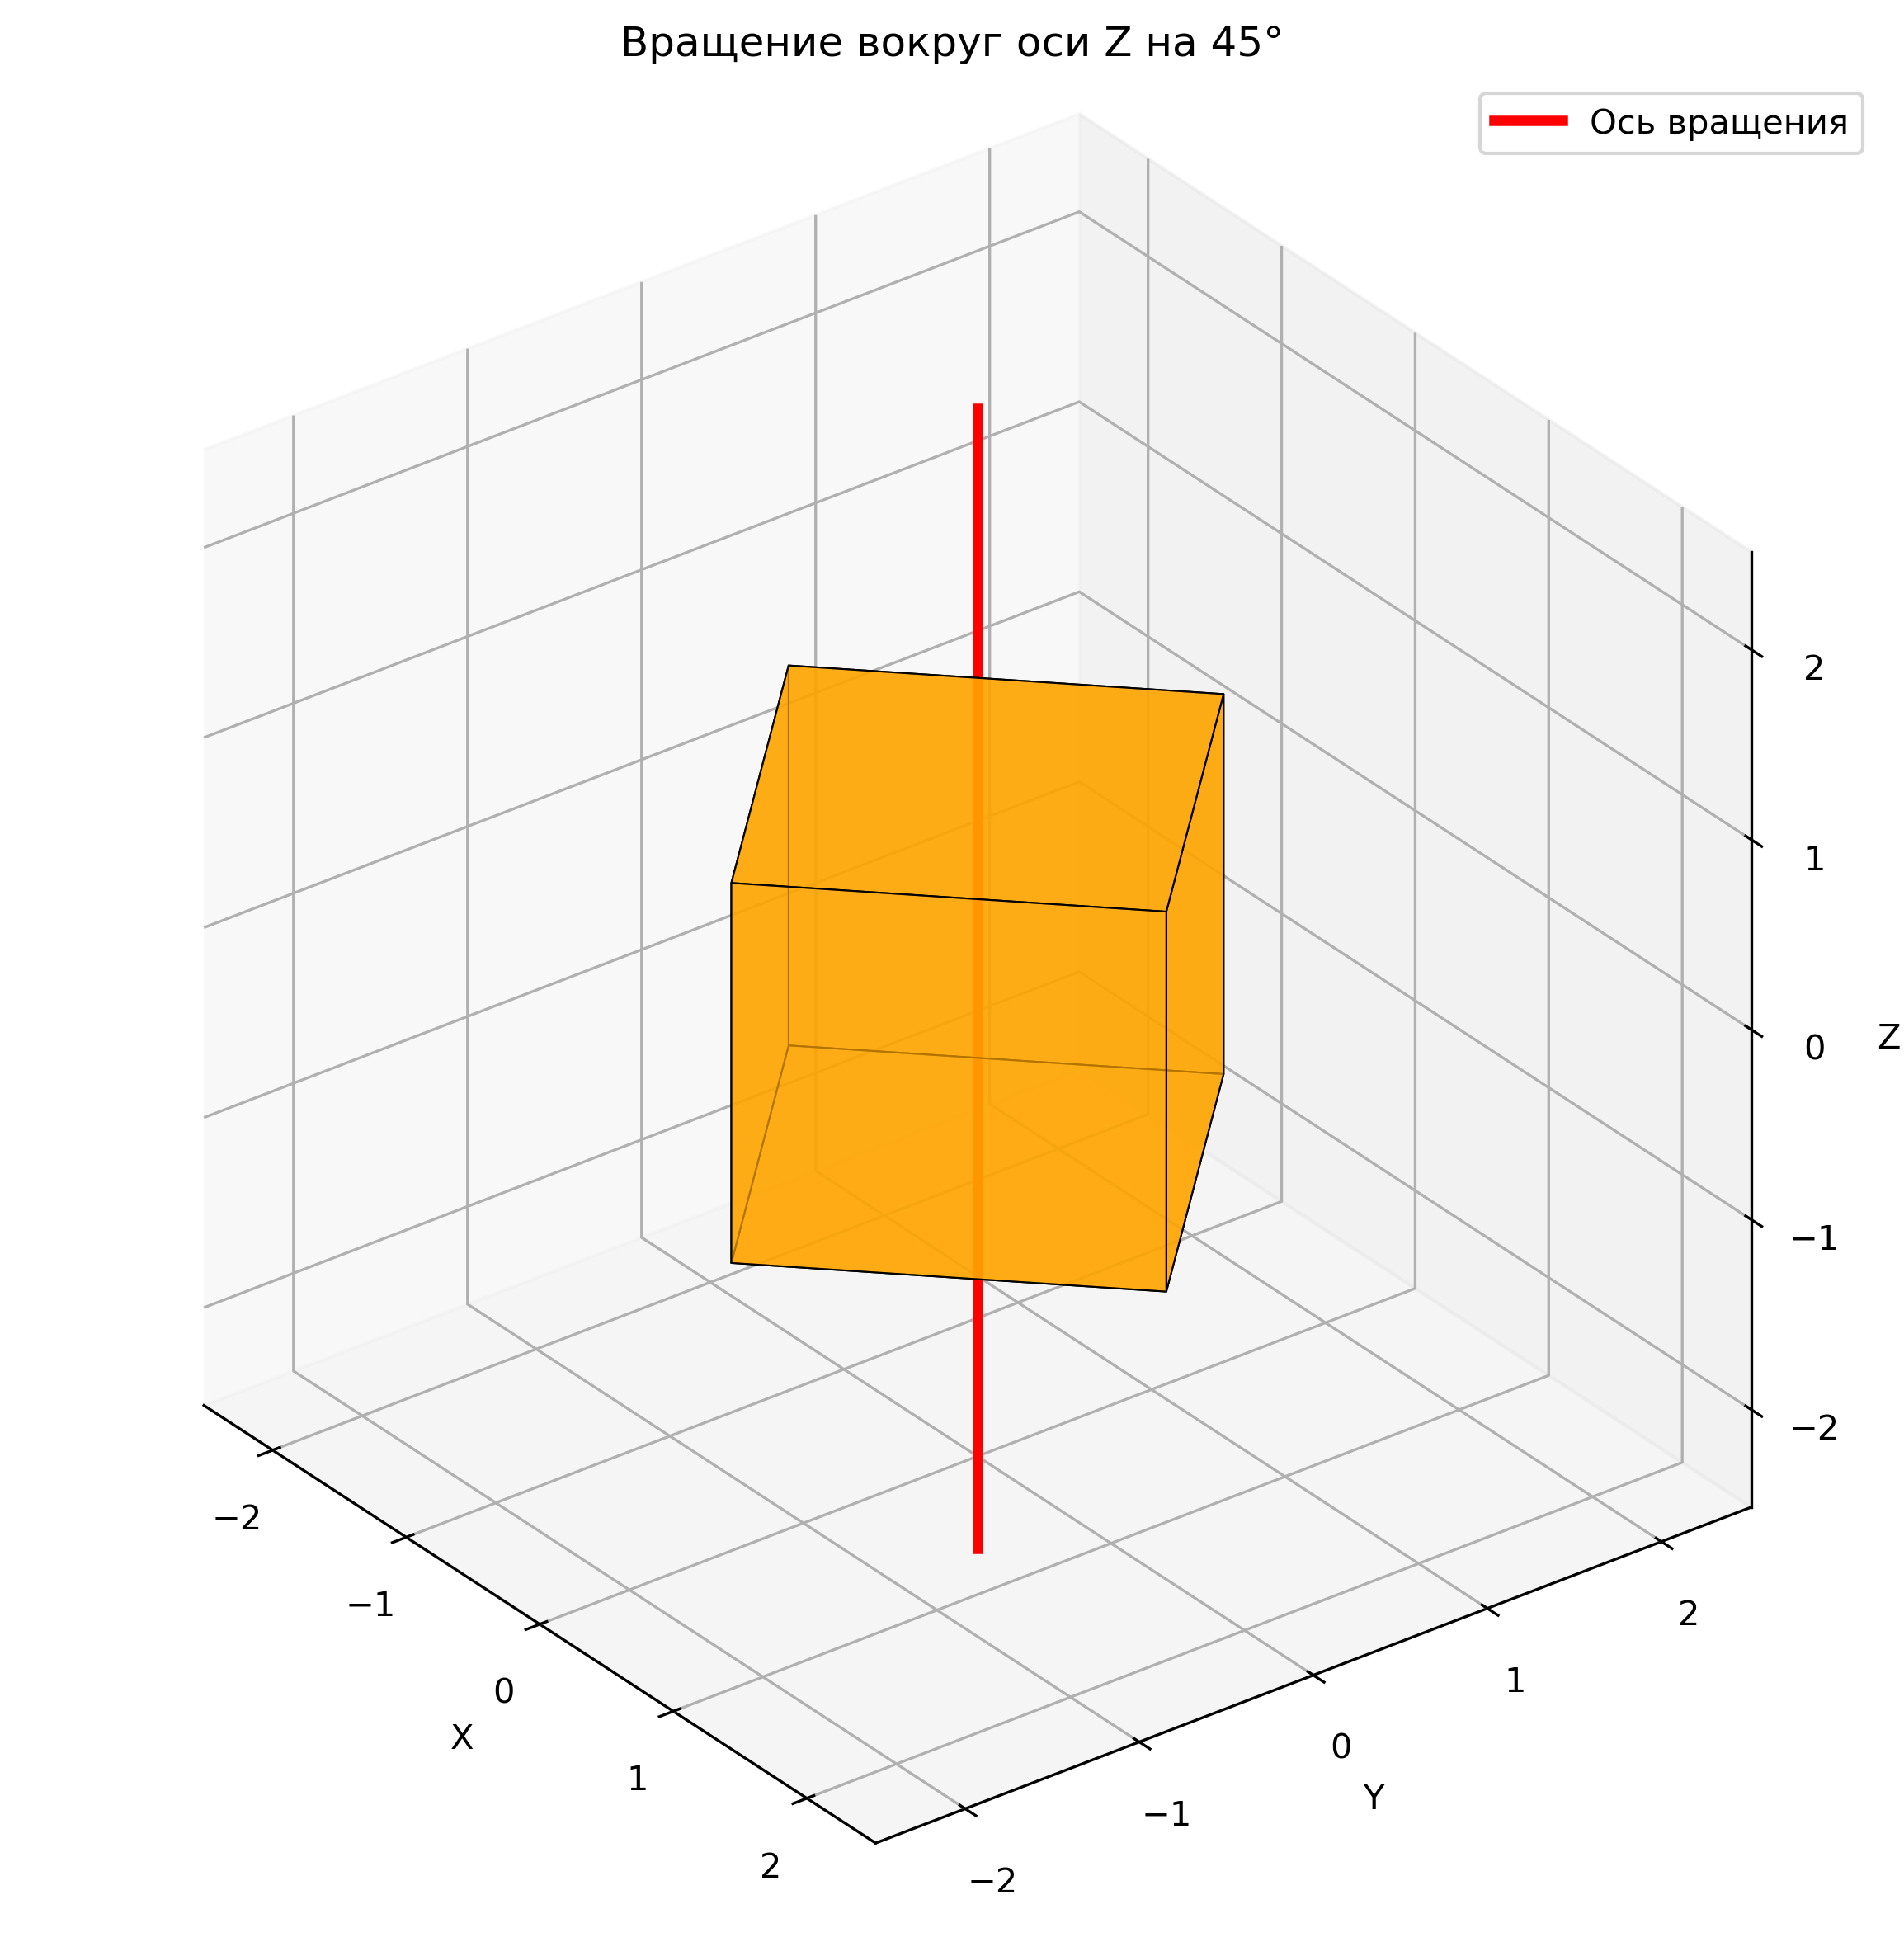
\includegraphics[width=0.8\textwidth]{images/task4/rotate_z.png}
\caption{Вращение вокруг оси Z на 45°}
\end{figure}

\begin{figure}[H]
\centering
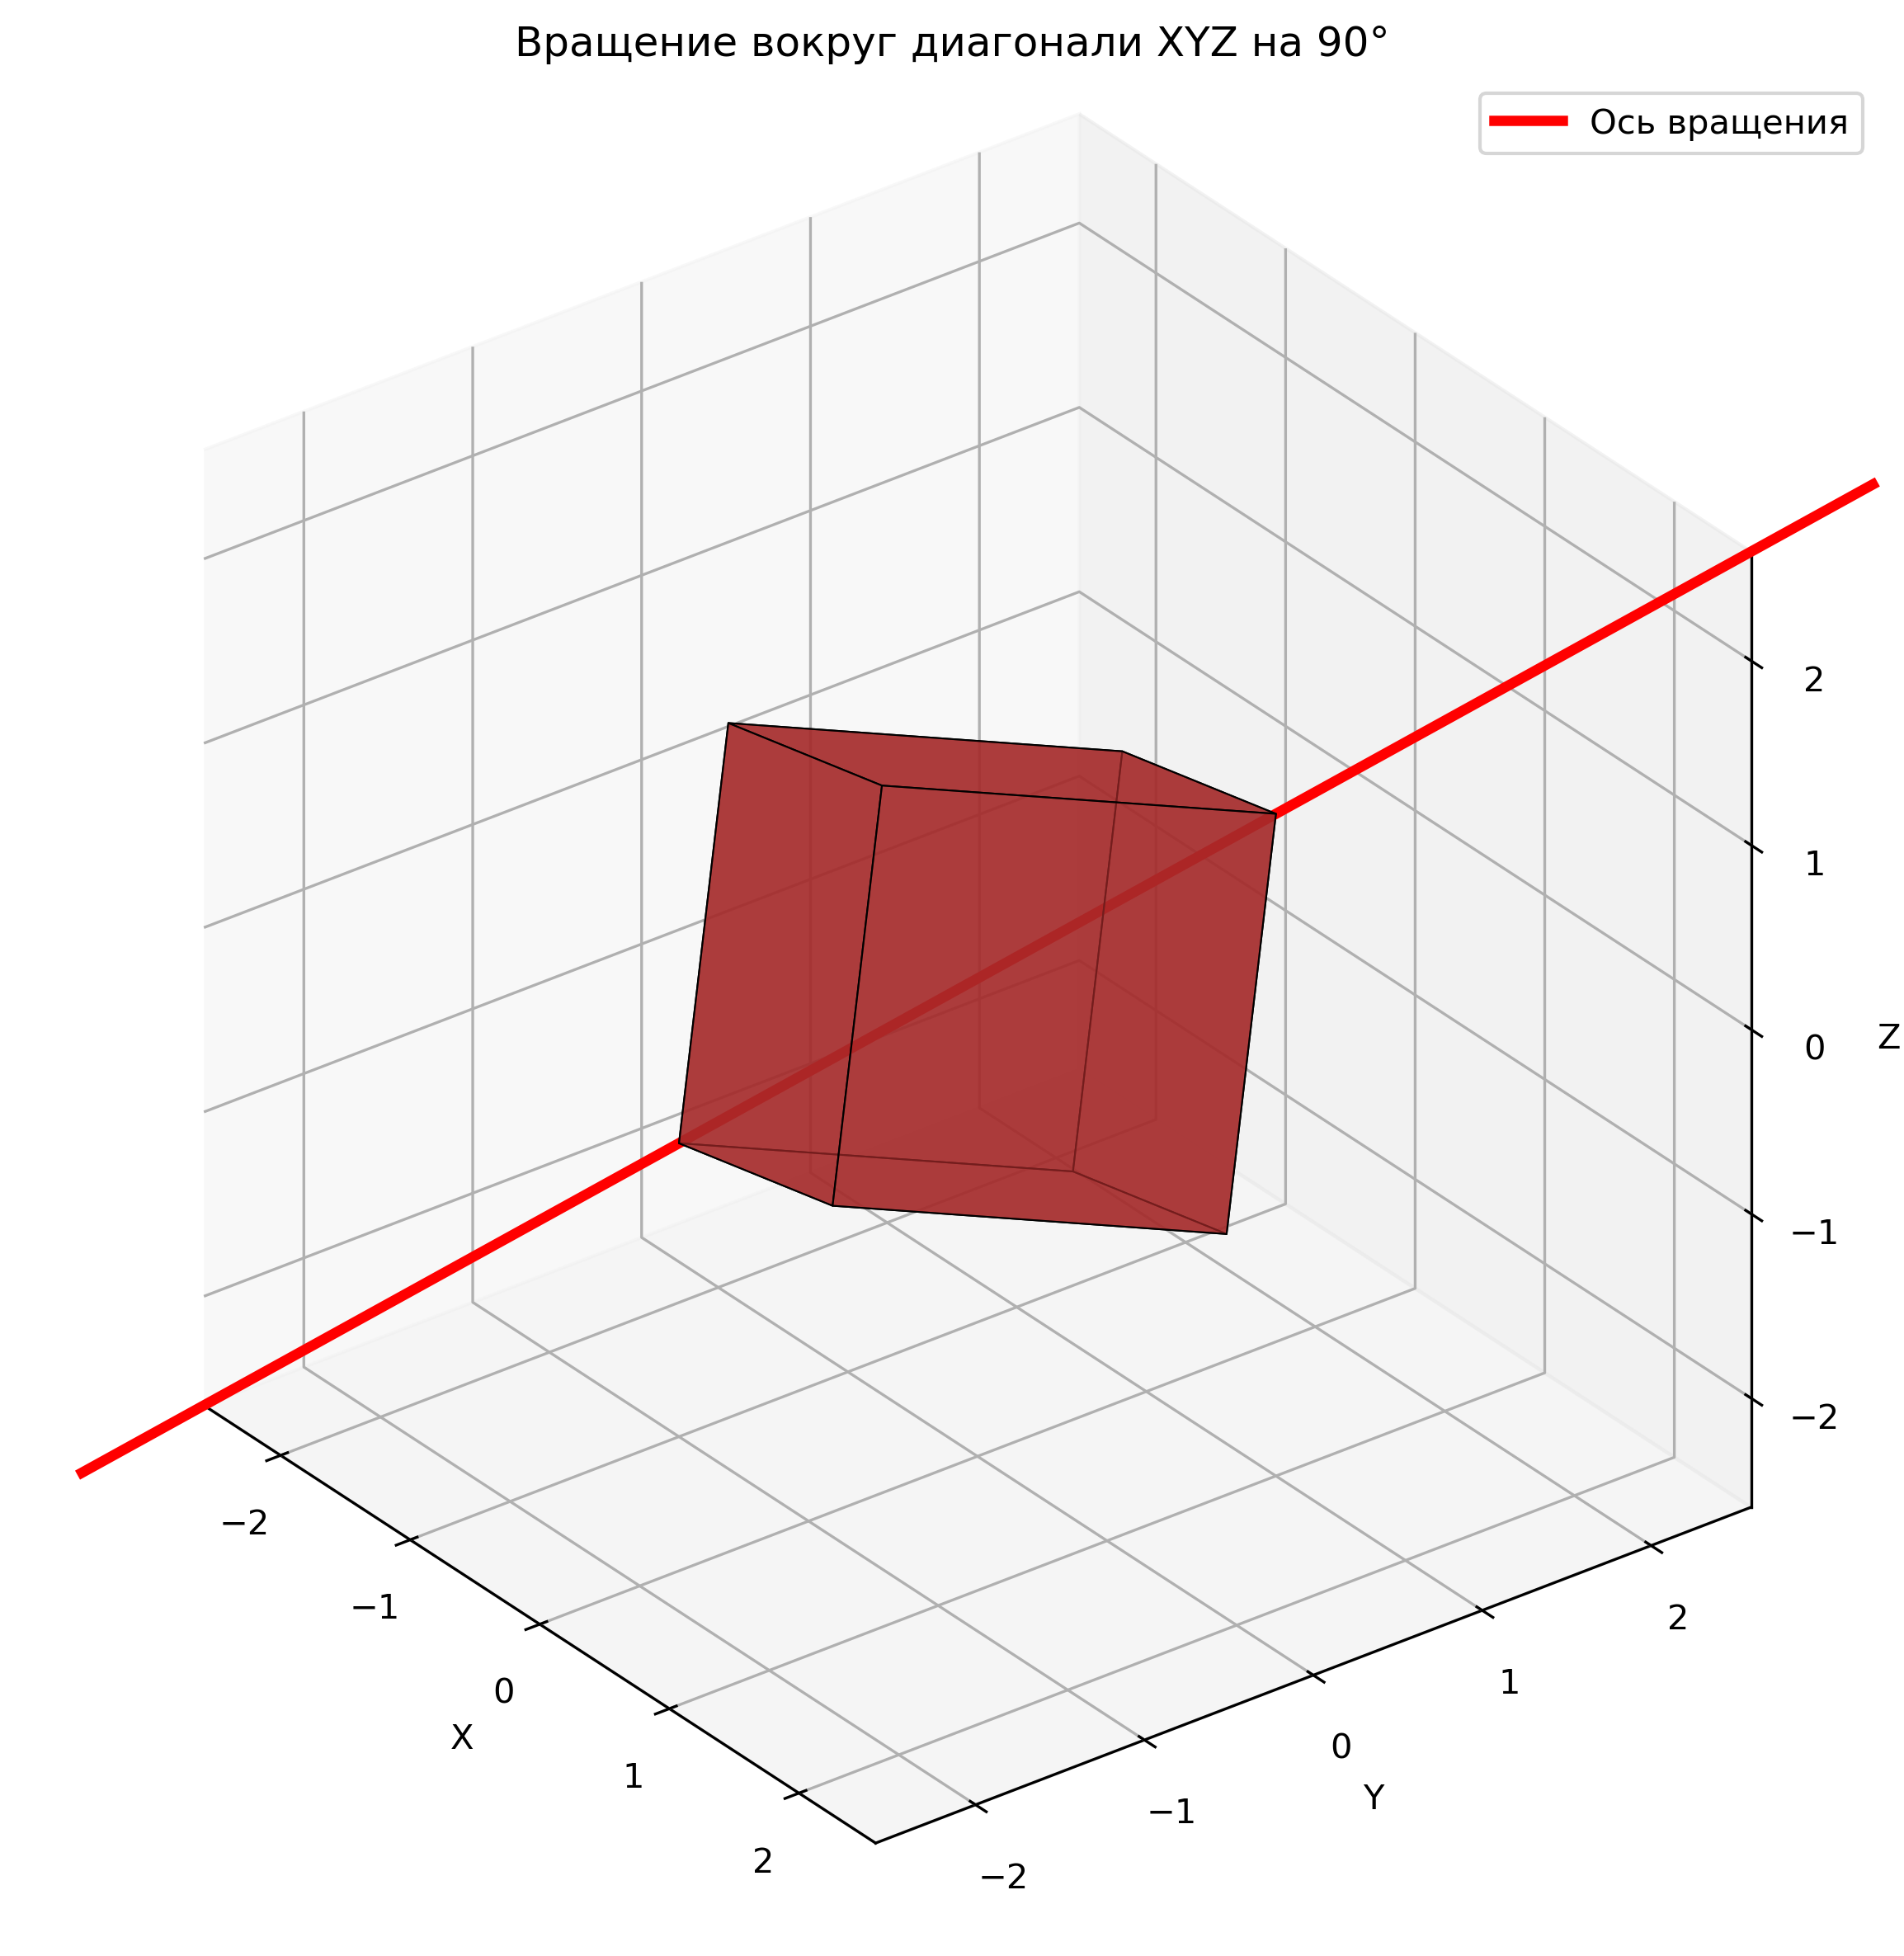
\includegraphics[width=0.8\textwidth]{images/task4/rotate_xyz.png}
\caption{Вращение вокруг диагонали XYZ на 90°}
\end{figure}

\begin{figure}[H]
\centering
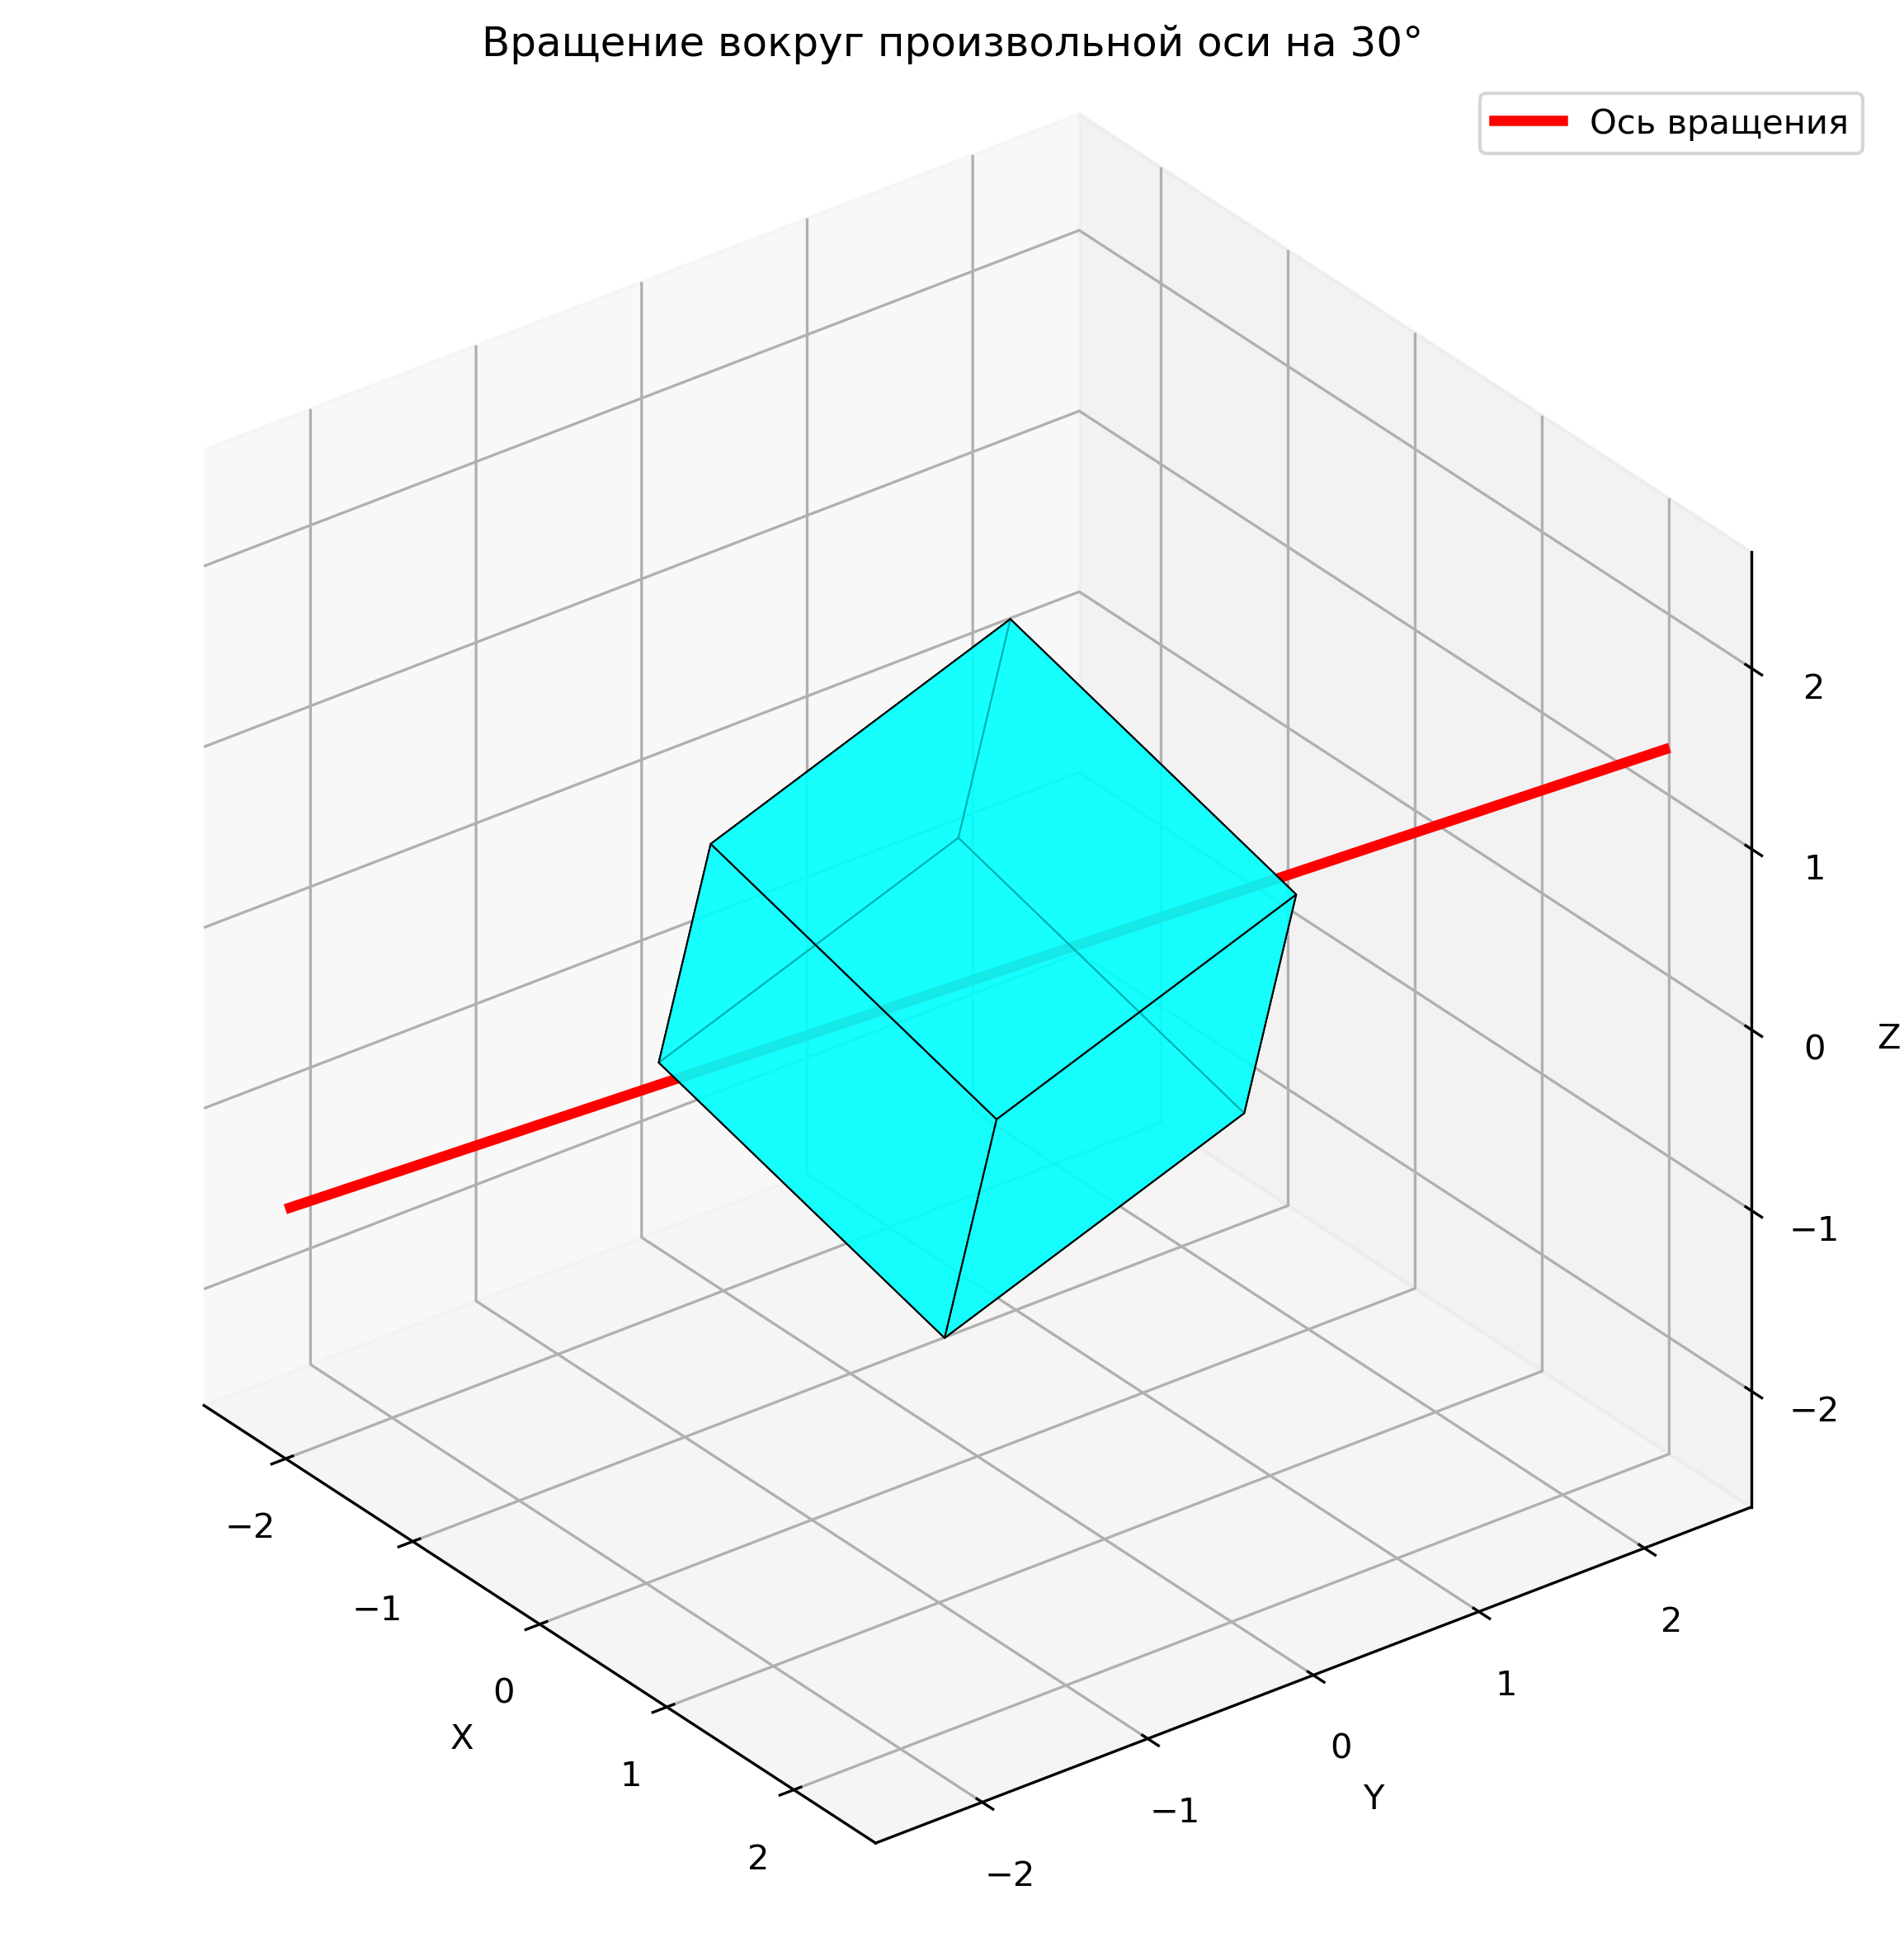
\includegraphics[width=0.8\textwidth]{images/task4/rotate_arbitrary.png}
\caption{Вращение вокруг произвольной оси на 30°}
\end{figure}

\subsection*{Сравнение с вращениями вокруг осей координат}

\begin{figure}[H]
\centering
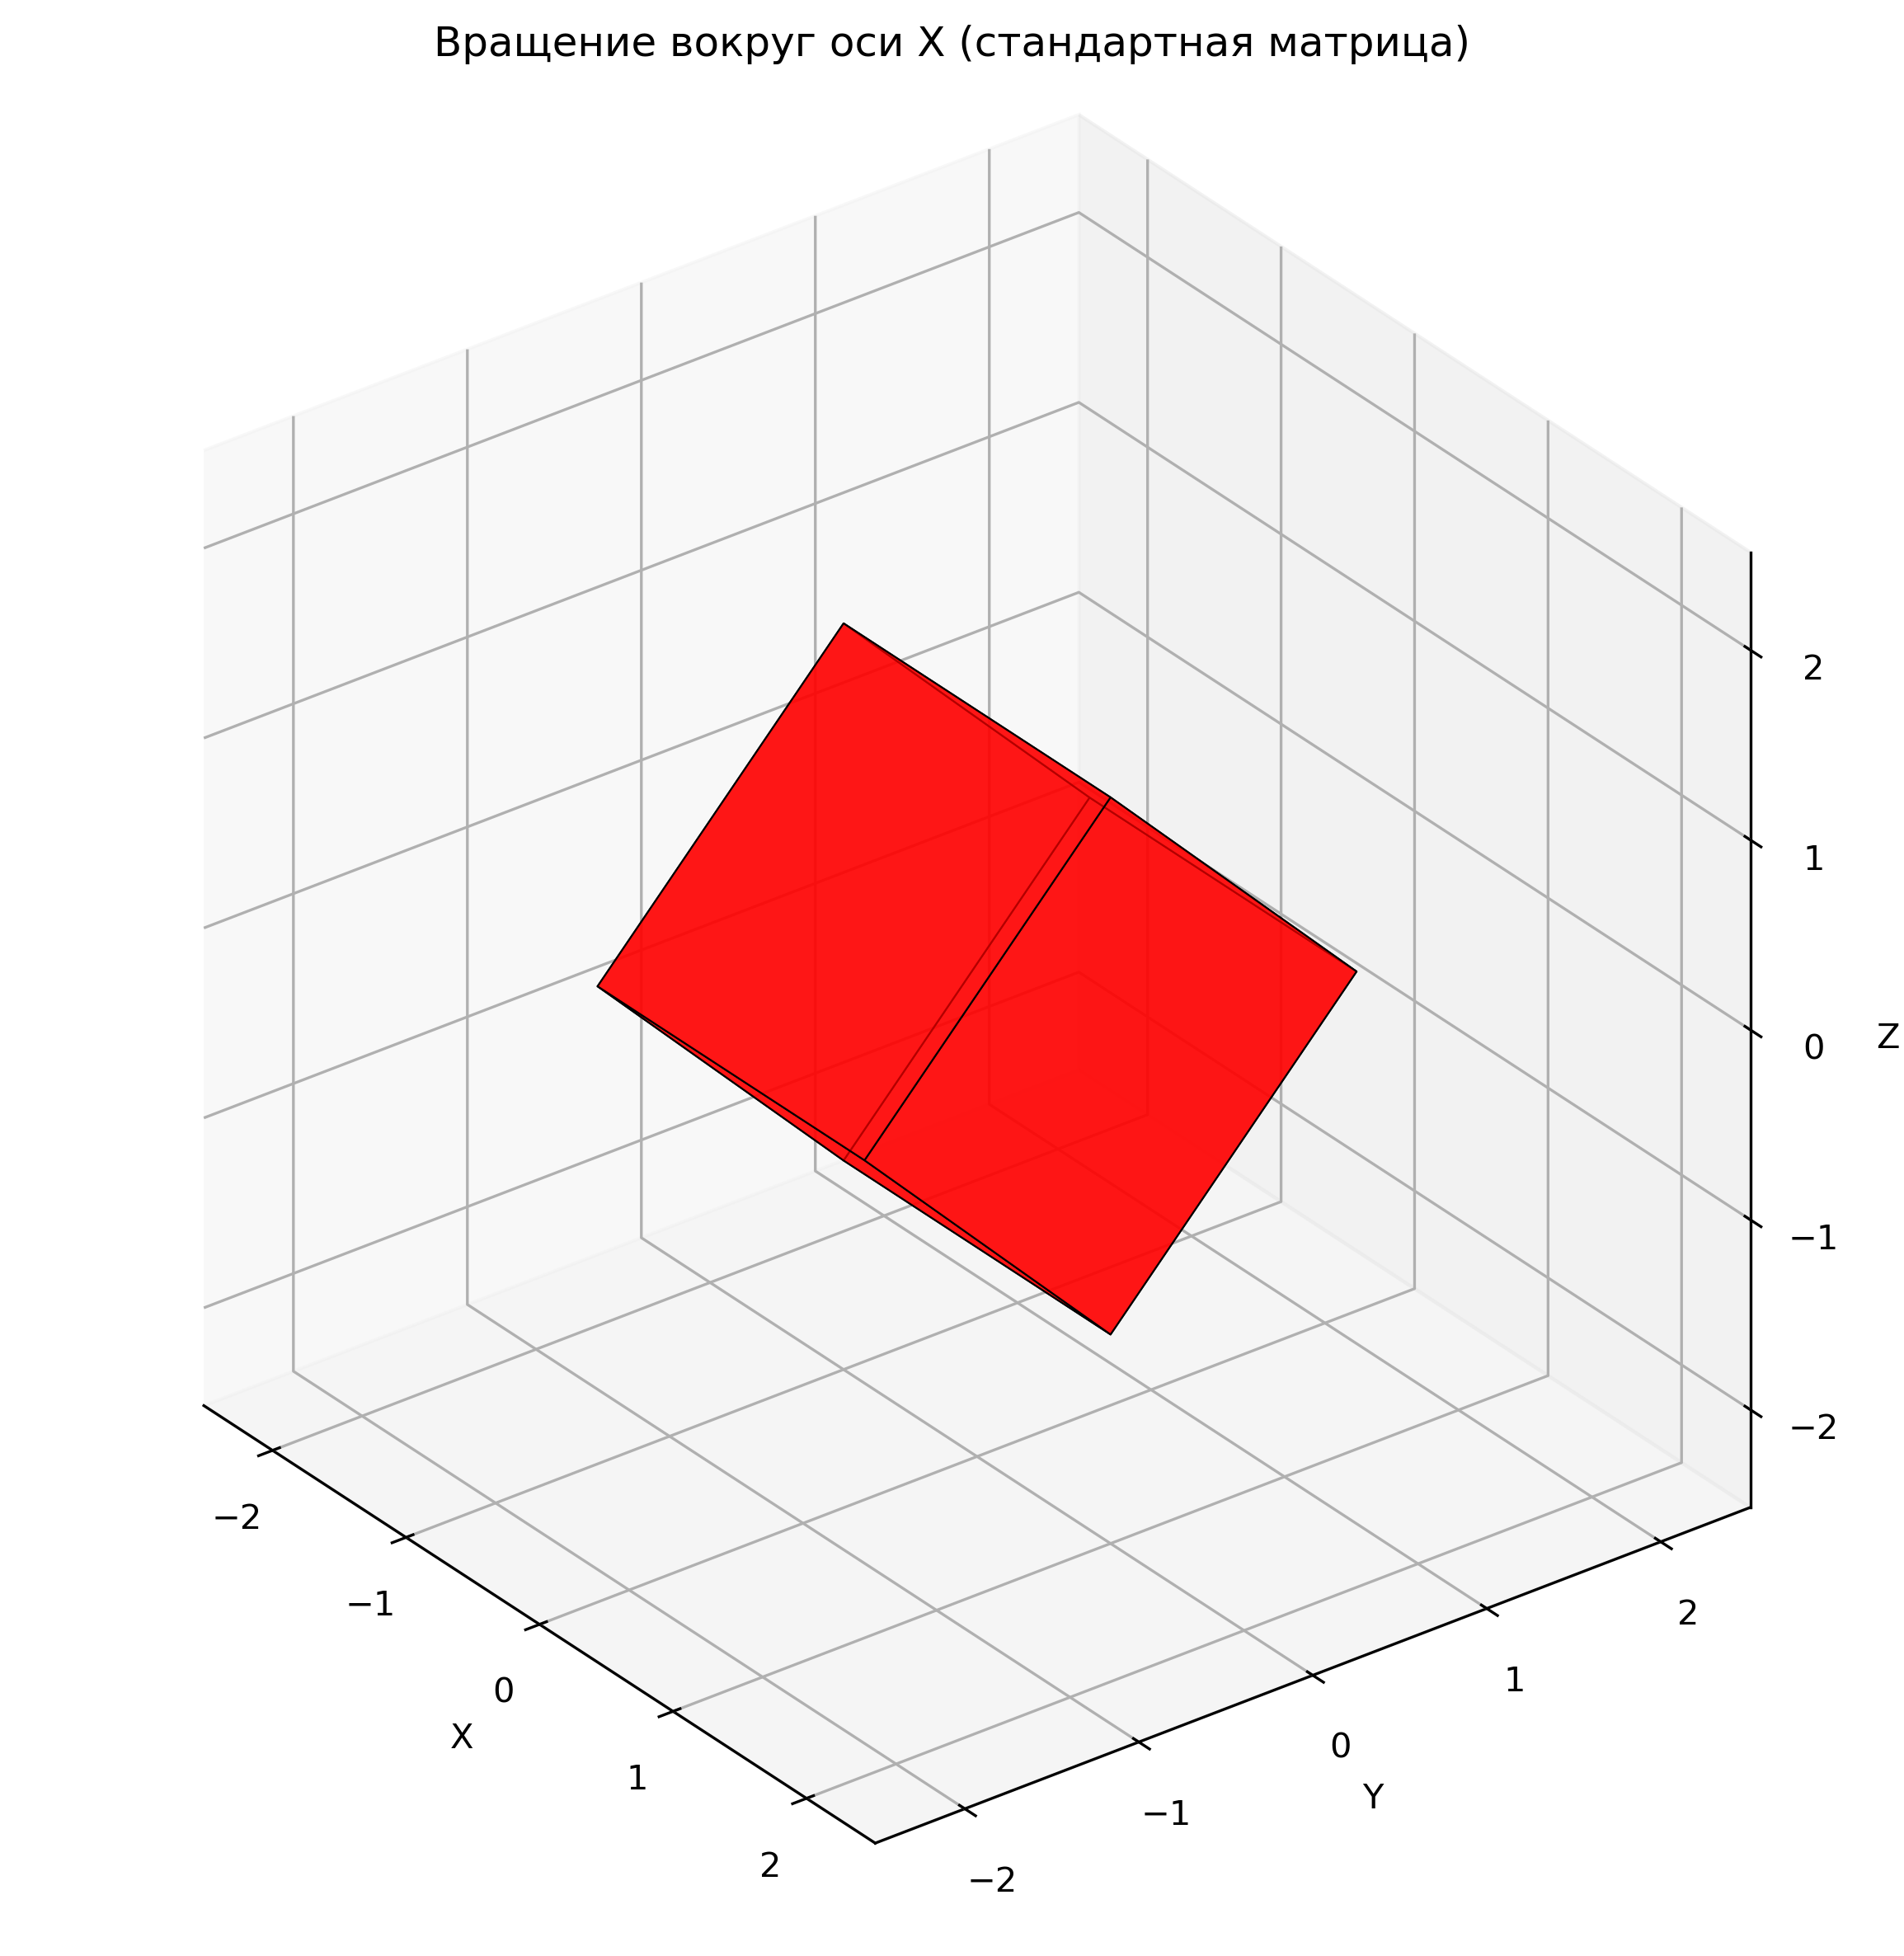
\includegraphics[width=0.8\textwidth]{images/task4/rotate_x_standard.png}
\caption{Вращение вокруг оси X (стандартная матрица)}
\end{figure}

\begin{figure}[H]
\centering
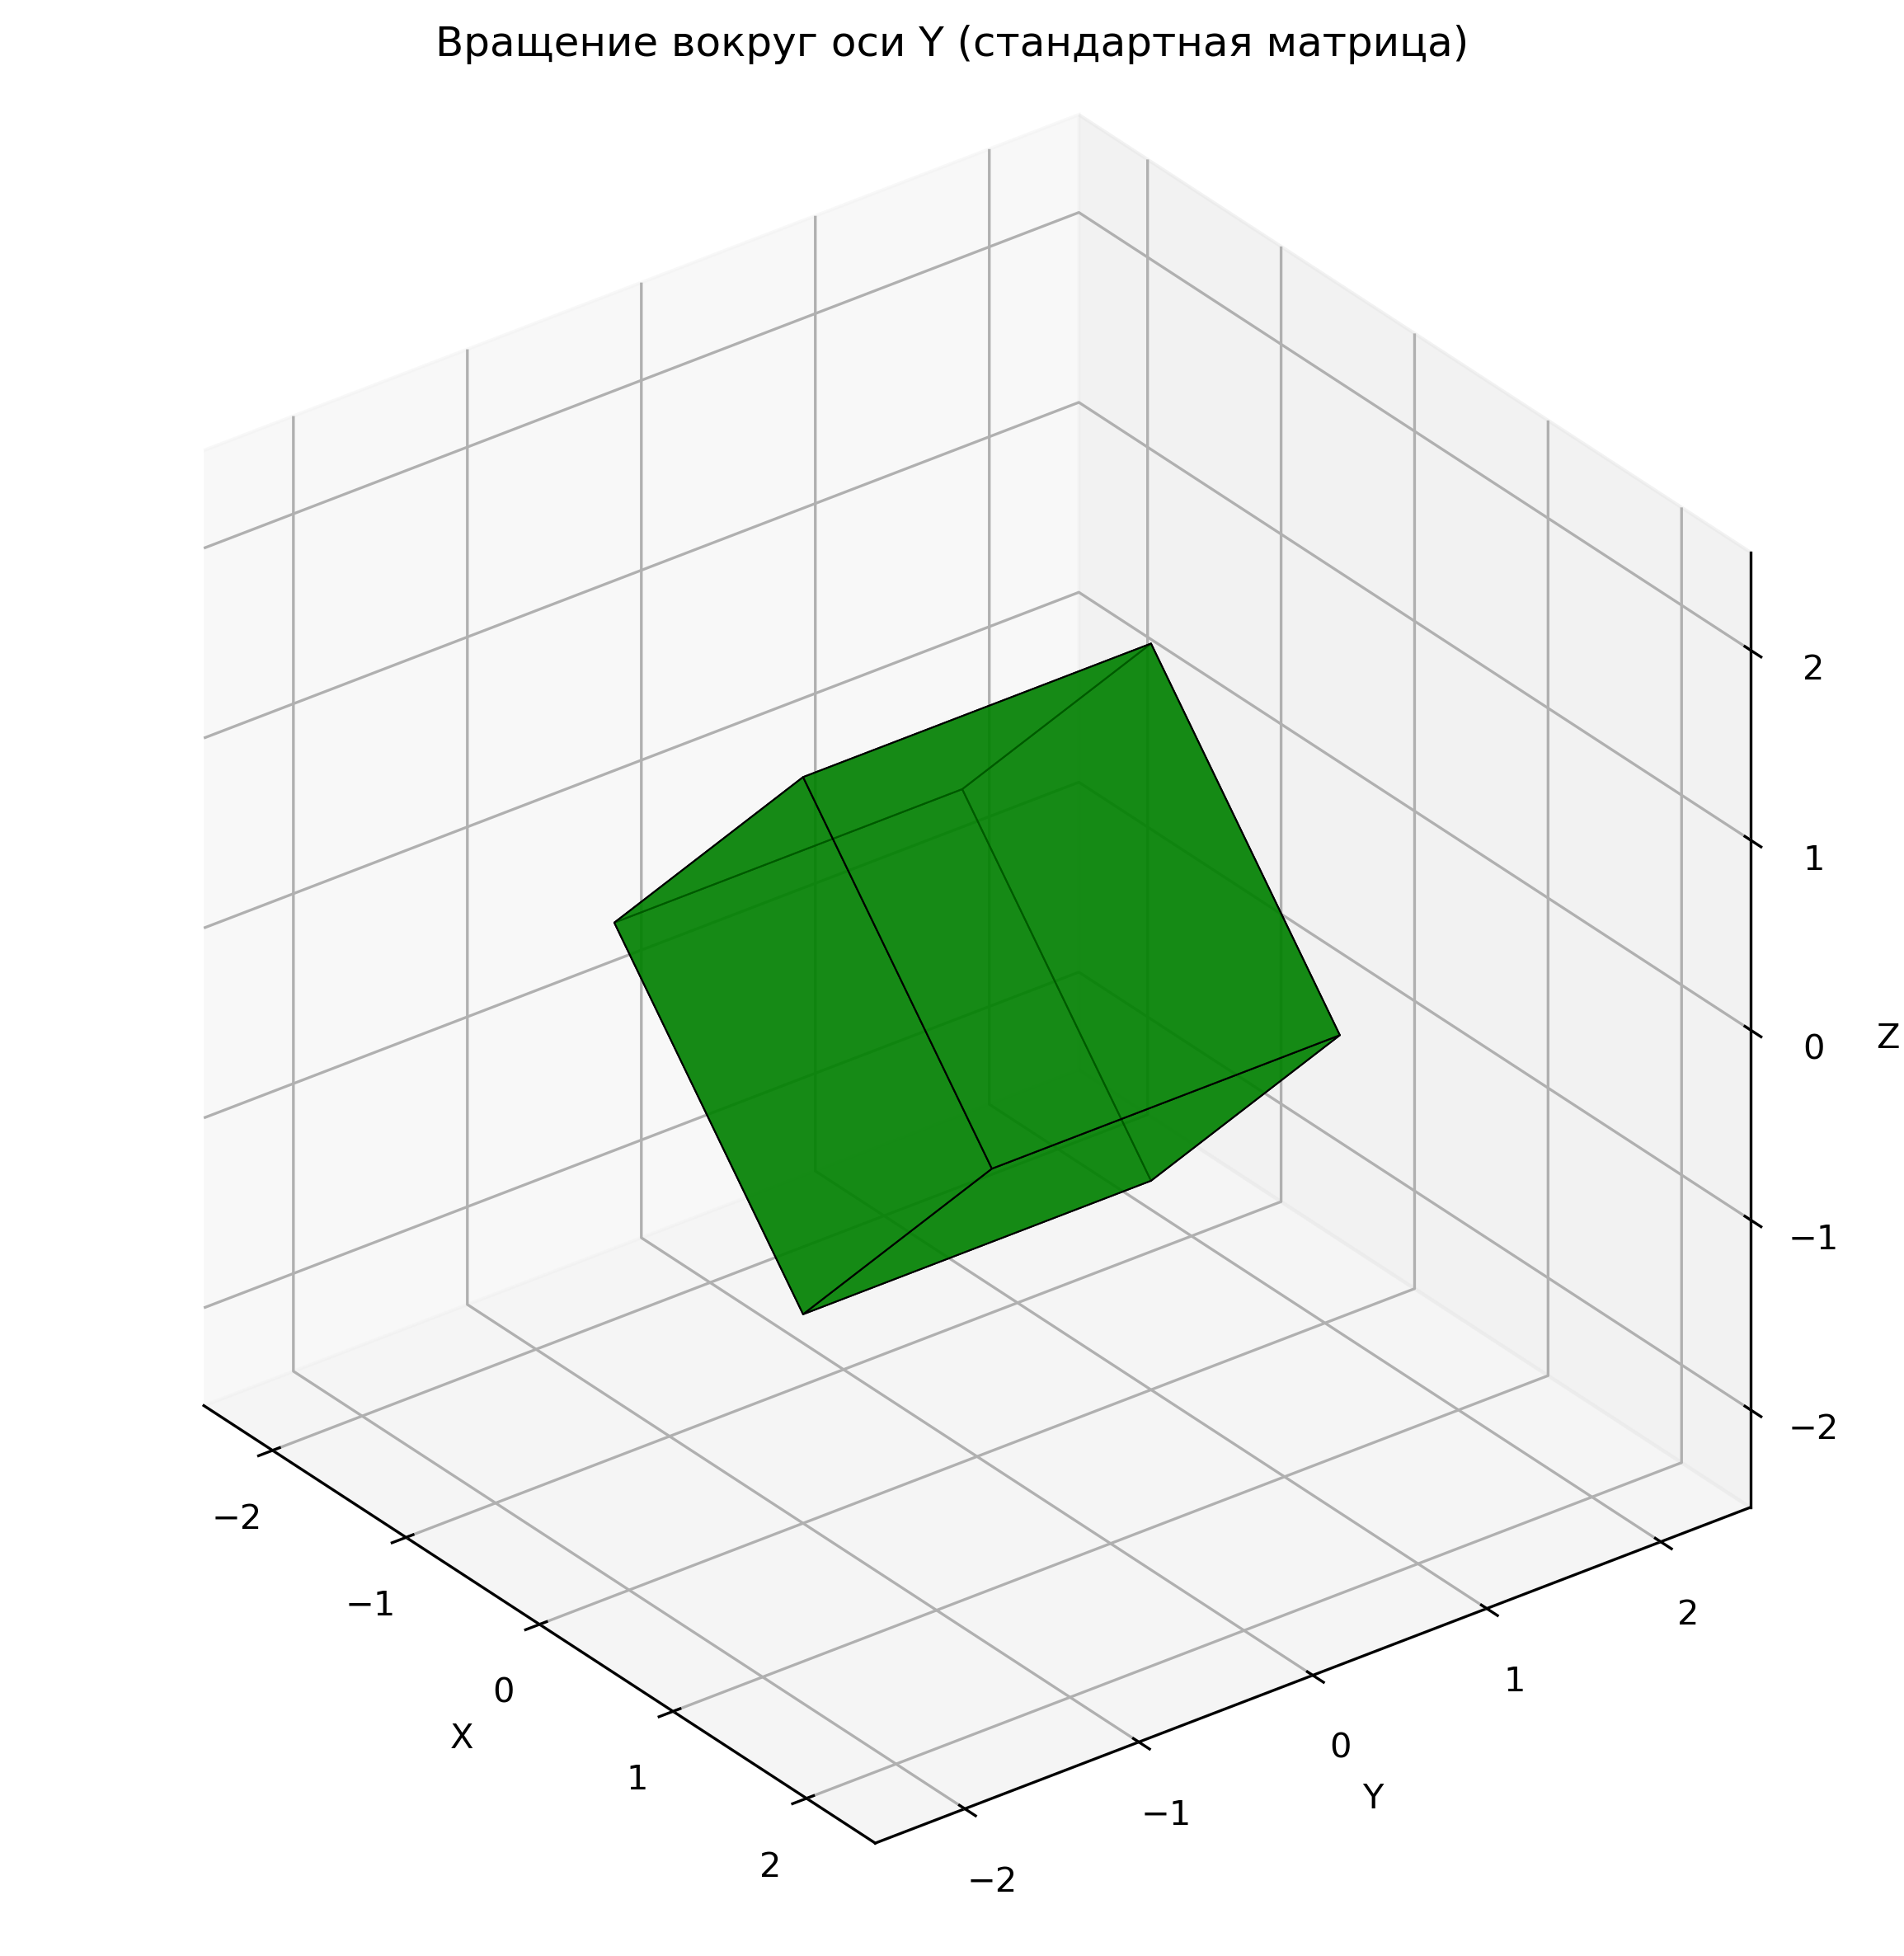
\includegraphics[width=0.8\textwidth]{images/task4/rotate_y_standard.png}
\caption{Вращение вокруг оси Y (стандартная матрица)}
\end{figure}

\begin{figure}[H]
\centering
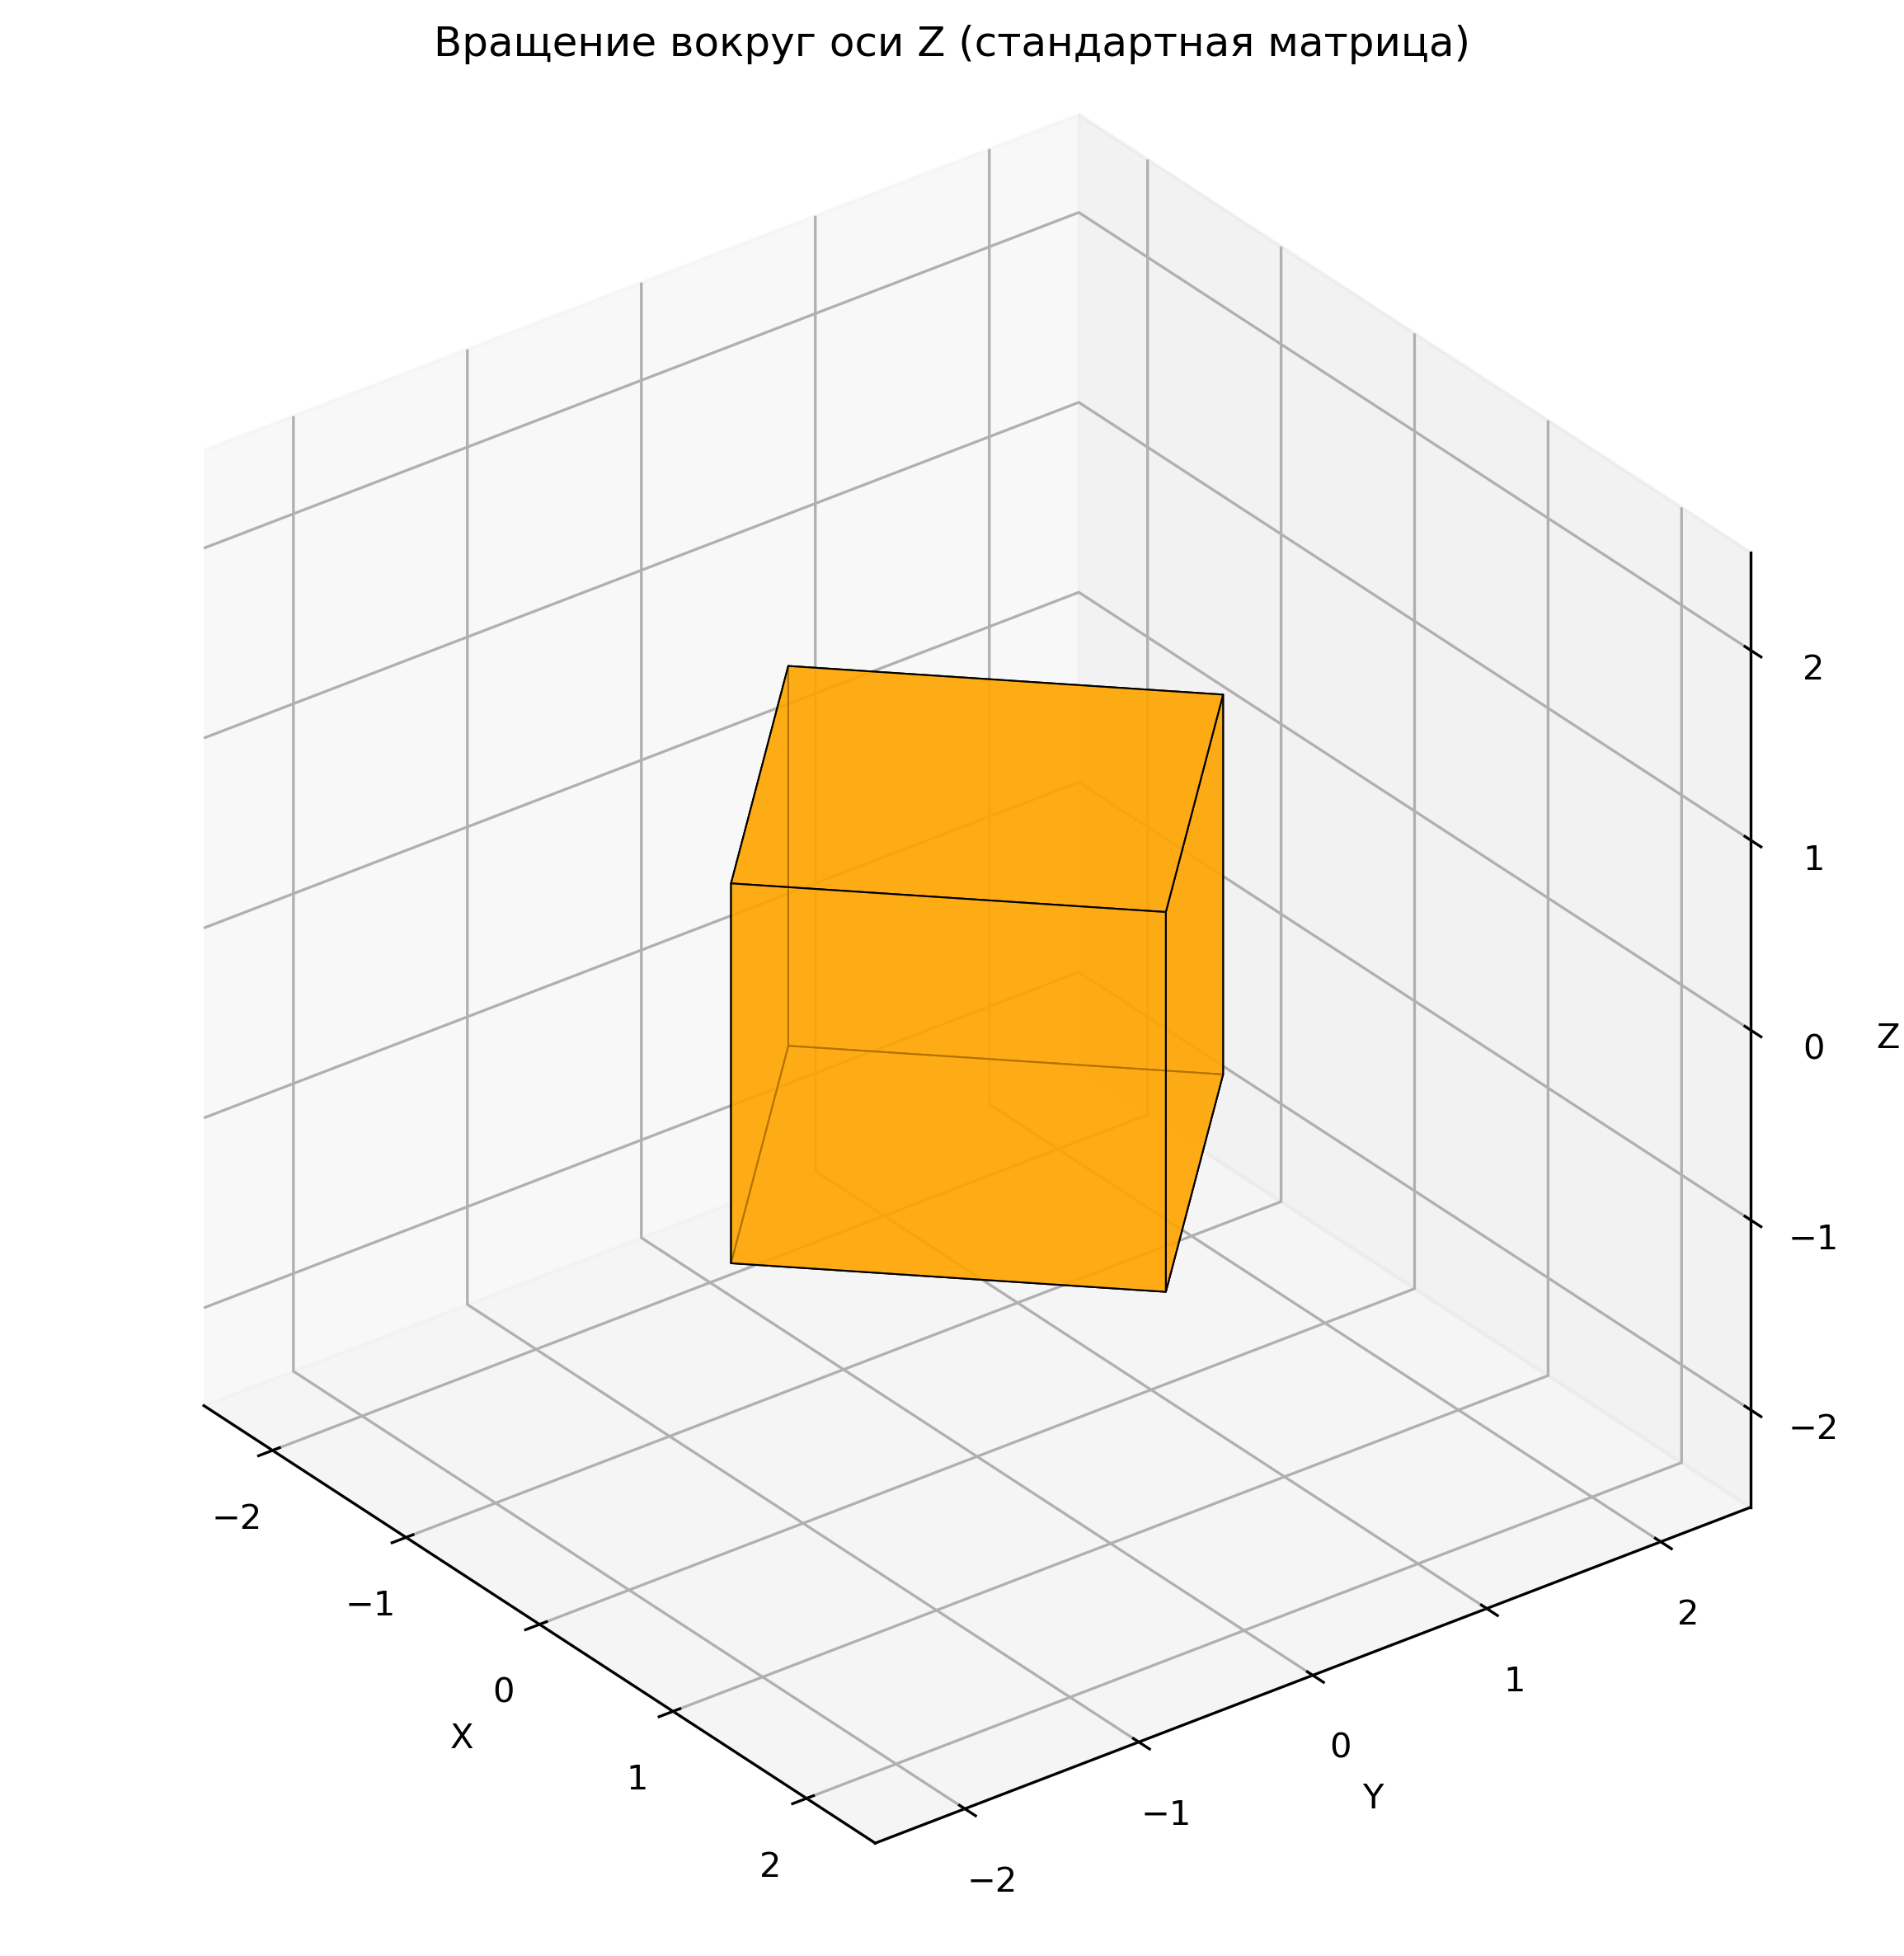
\includegraphics[width=0.8\textwidth]{images/task4/rotate_z_standard.png}
\caption{Вращение вокруг оси Z (стандартная матрица)}
\end{figure}

\subsection*{Теорема вращения Эйлера}
Исследована композиция вращений $R_x(\theta) \cdot R_y(\phi) \cdot R_z(\psi)$:

\begin{itemize}
    \item Любое вращение в 3D можно представить как вращение вокруг одной оси
    \item Композиция $R_x(\theta)R_y(\phi)R_z(\psi)$ не покрывает все возможные вращения
    \item Для полного покрытия нужны другие параметризации (например, кватернионы)
\end{itemize}

\section*{Задание 5: Вращение кубика около одной вершины}

\subsection*{Постановка задачи}
Реализовать вращение кубика вокруг одной из его вершин и исследовать свойства такого преобразования.

\subsection*{Математические основы}
Вращение вокруг вершины выполняется в три этапа:
\begin{enumerate}
    \item Перемещение: $T_1$ - перемещение выбранной вершины в начало координат
    \item Вращение: $R$ - вращение вокруг оси
    \item Обратное перемещение: $T_2$ - возврат в исходное положение
\end{enumerate}

Полная матрица преобразования: $T_2 \cdot R \cdot T_1$

\subsection*{Результаты}
Исследованы вращения вокруг различных вершин:

\begin{figure}[H]
\centering
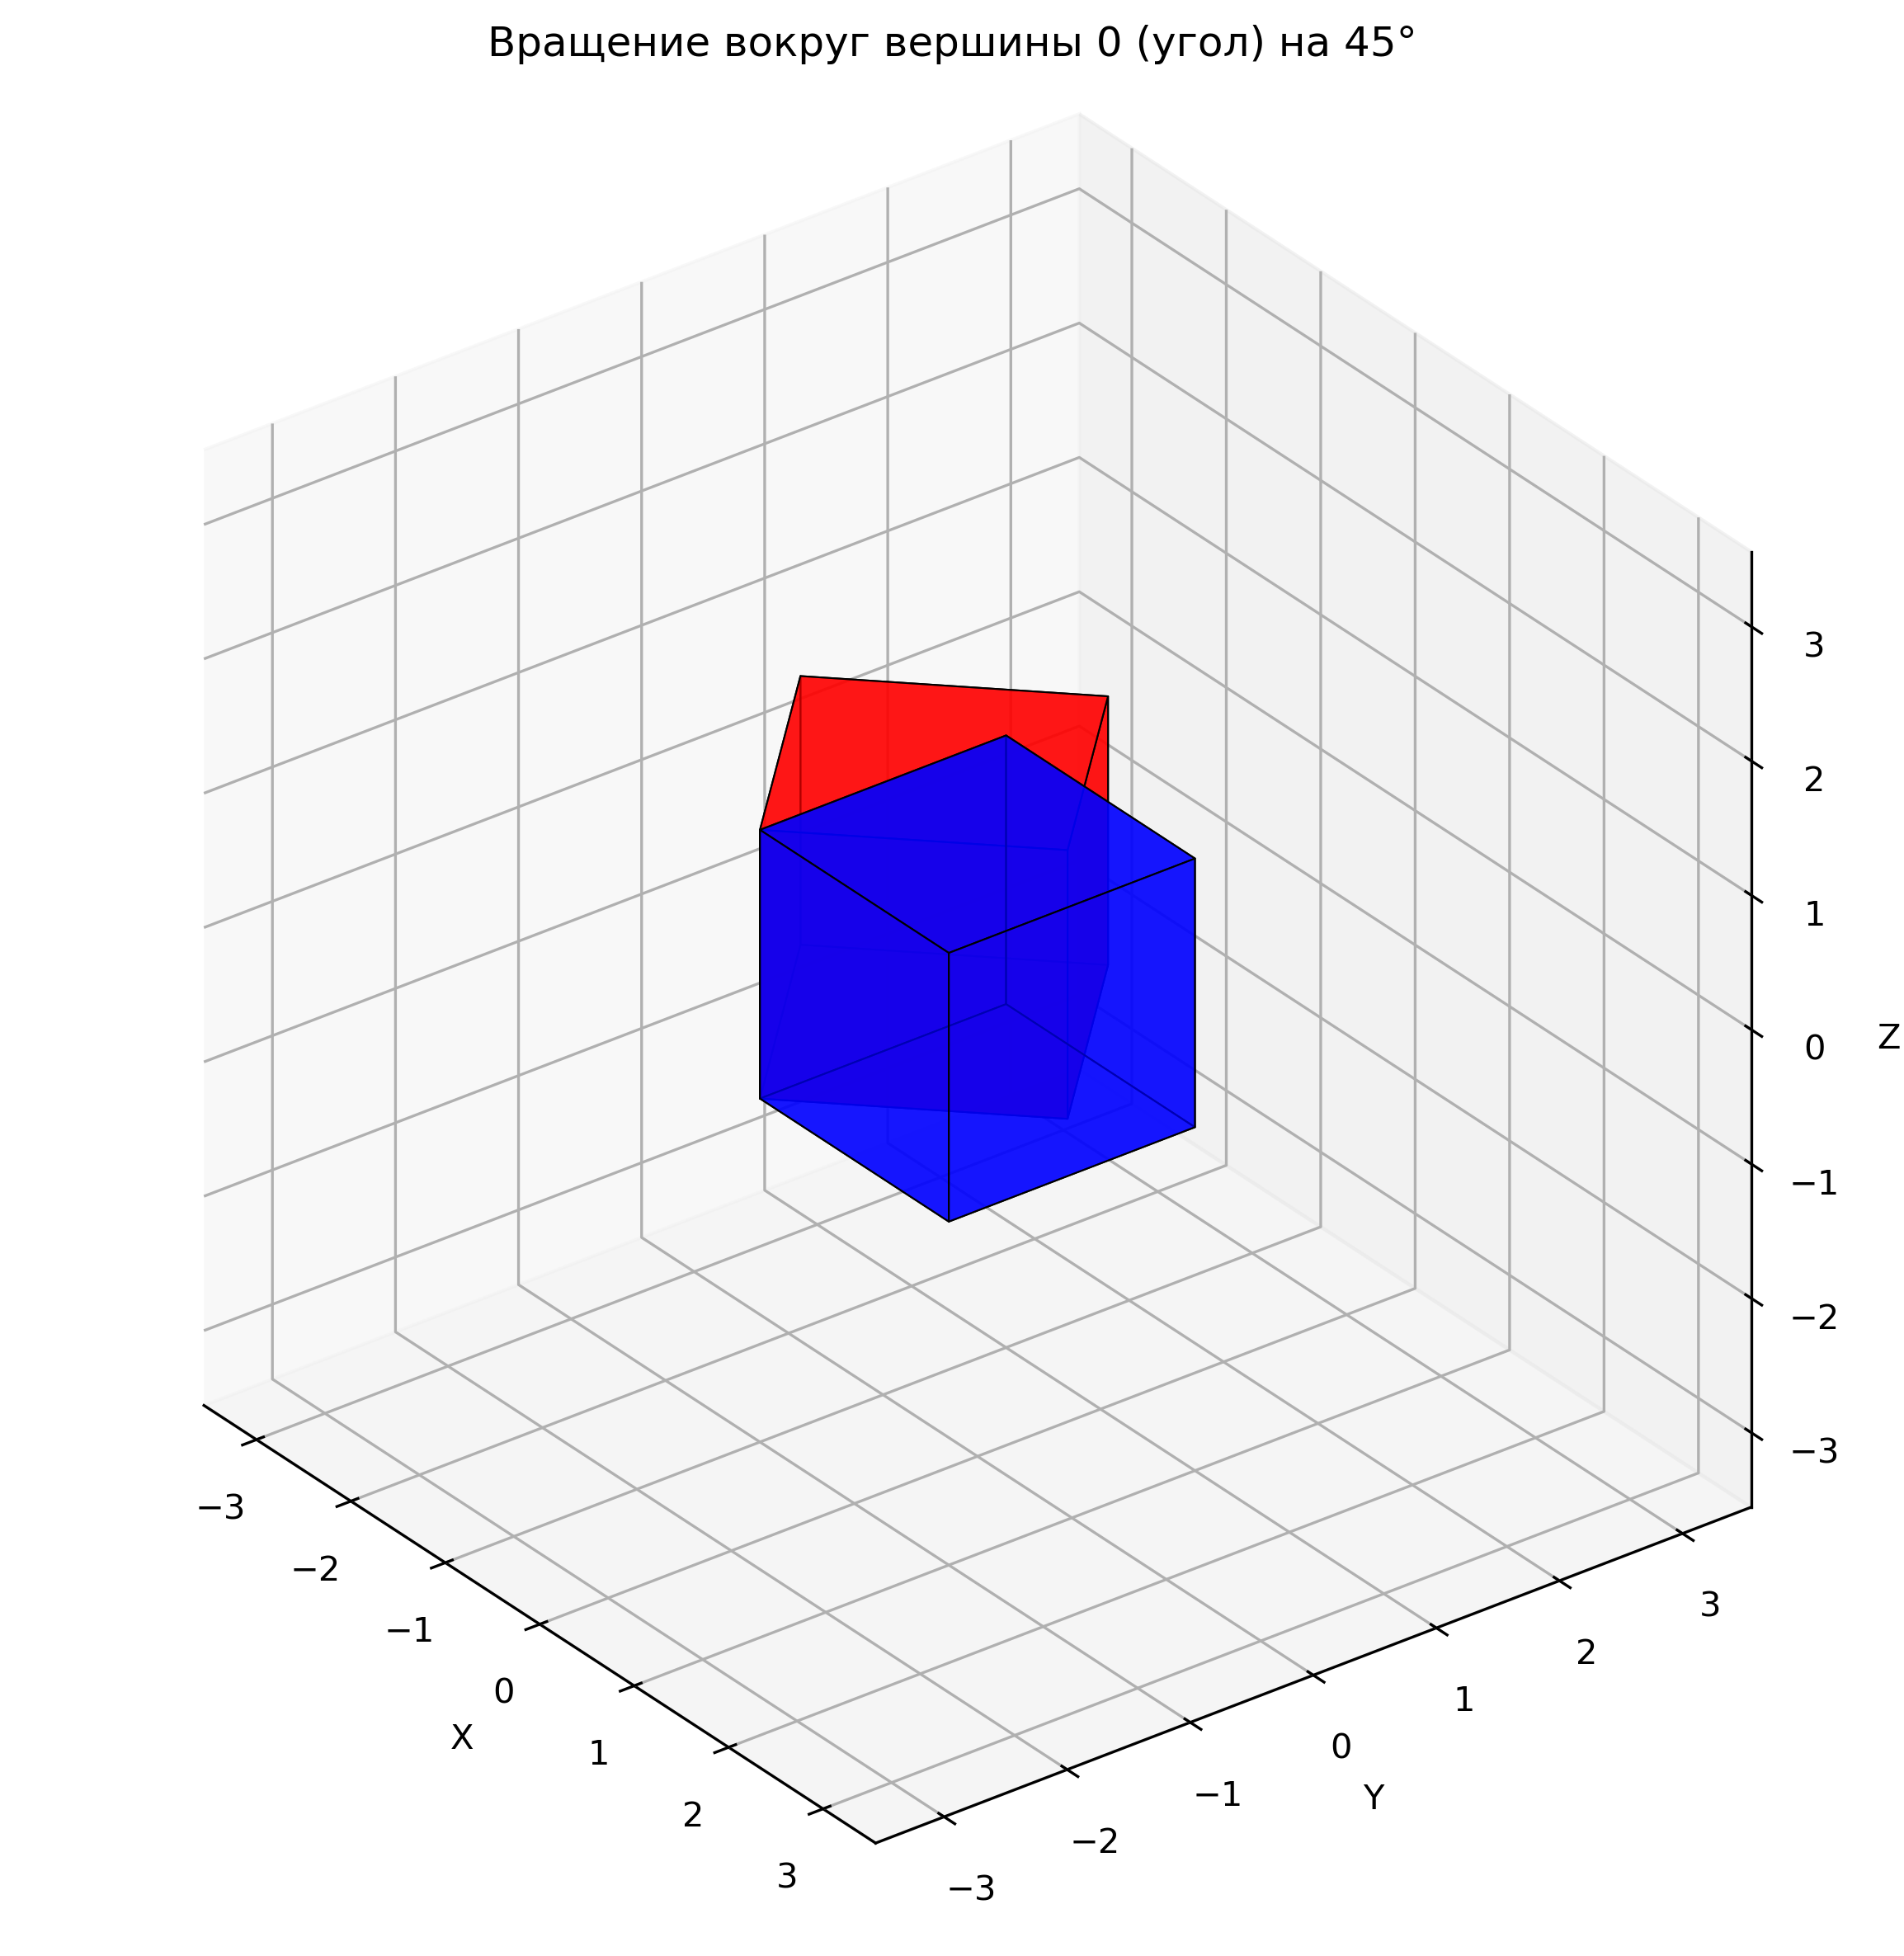
\includegraphics[width=0.8\textwidth]{images/task5/rotate_around_vertex_0.png}
\caption{Вращение вокруг вершины 0 (угол) на 45°}
\end{figure}

\begin{figure}[H]
\centering
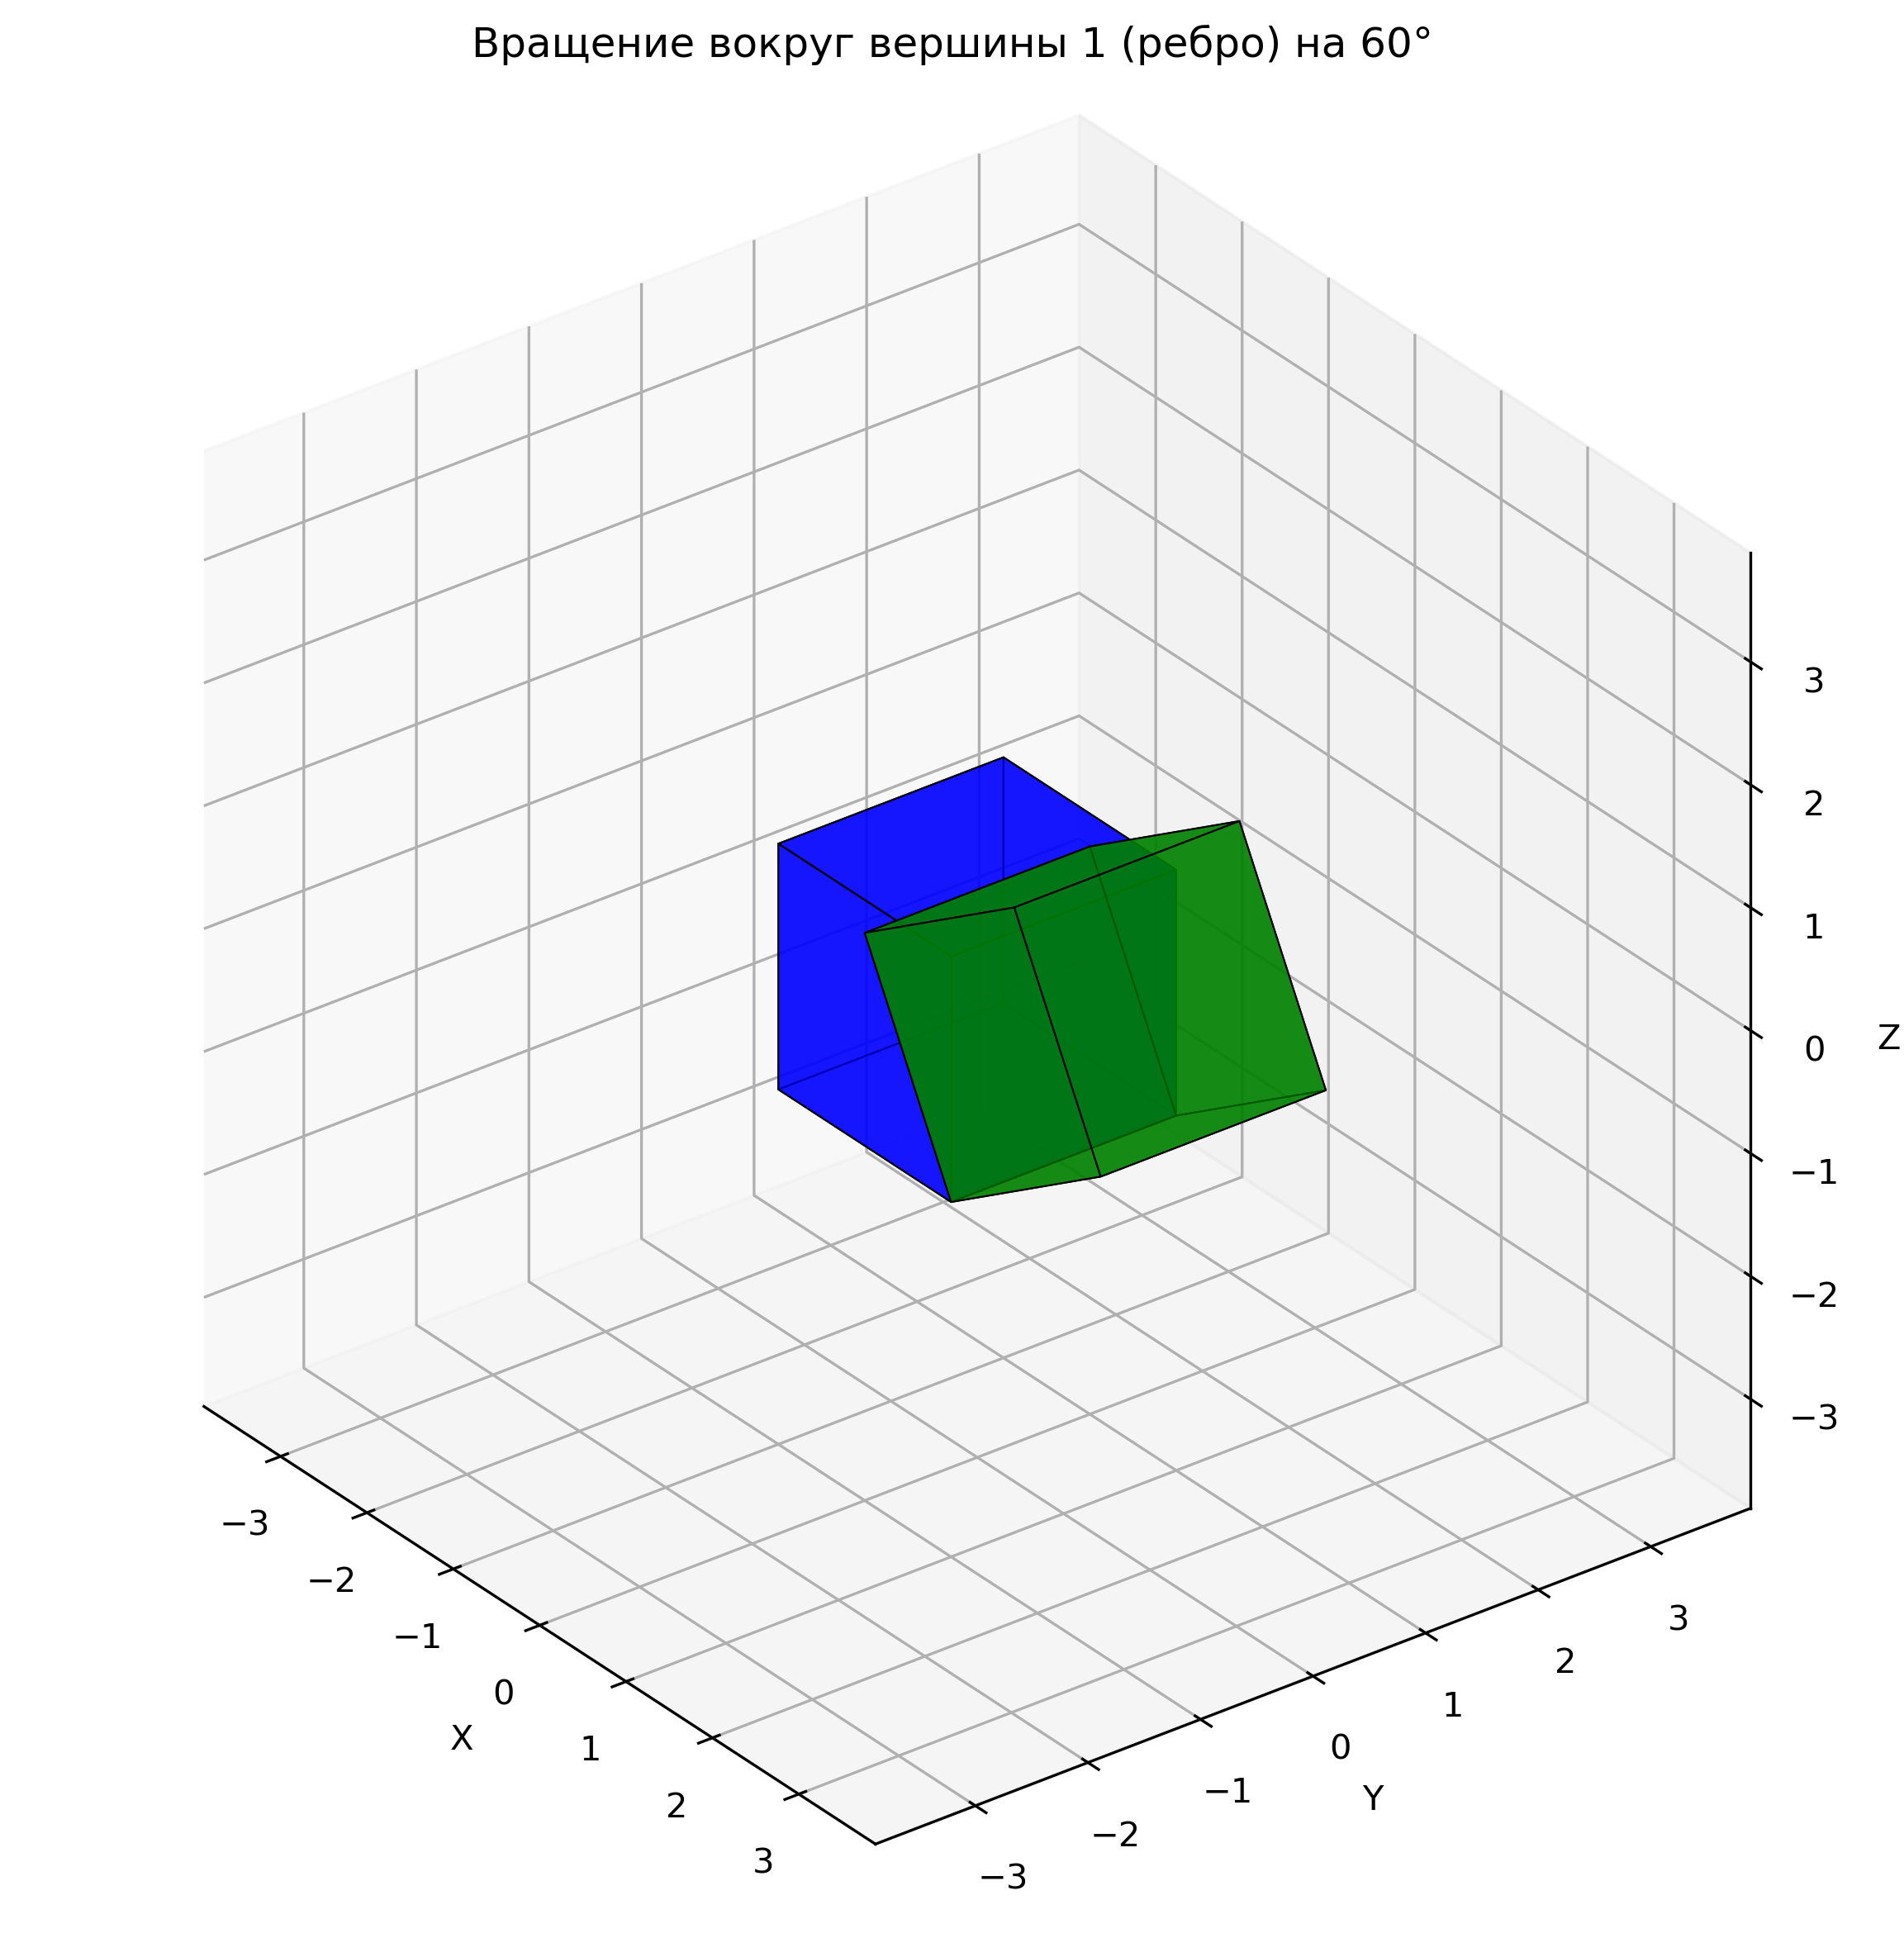
\includegraphics[width=0.8\textwidth]{images/task5/rotate_around_vertex_1.png}
\caption{Вращение вокруг вершины 1 (ребро) на 60°}
\end{figure}

\begin{figure}[H]
\centering
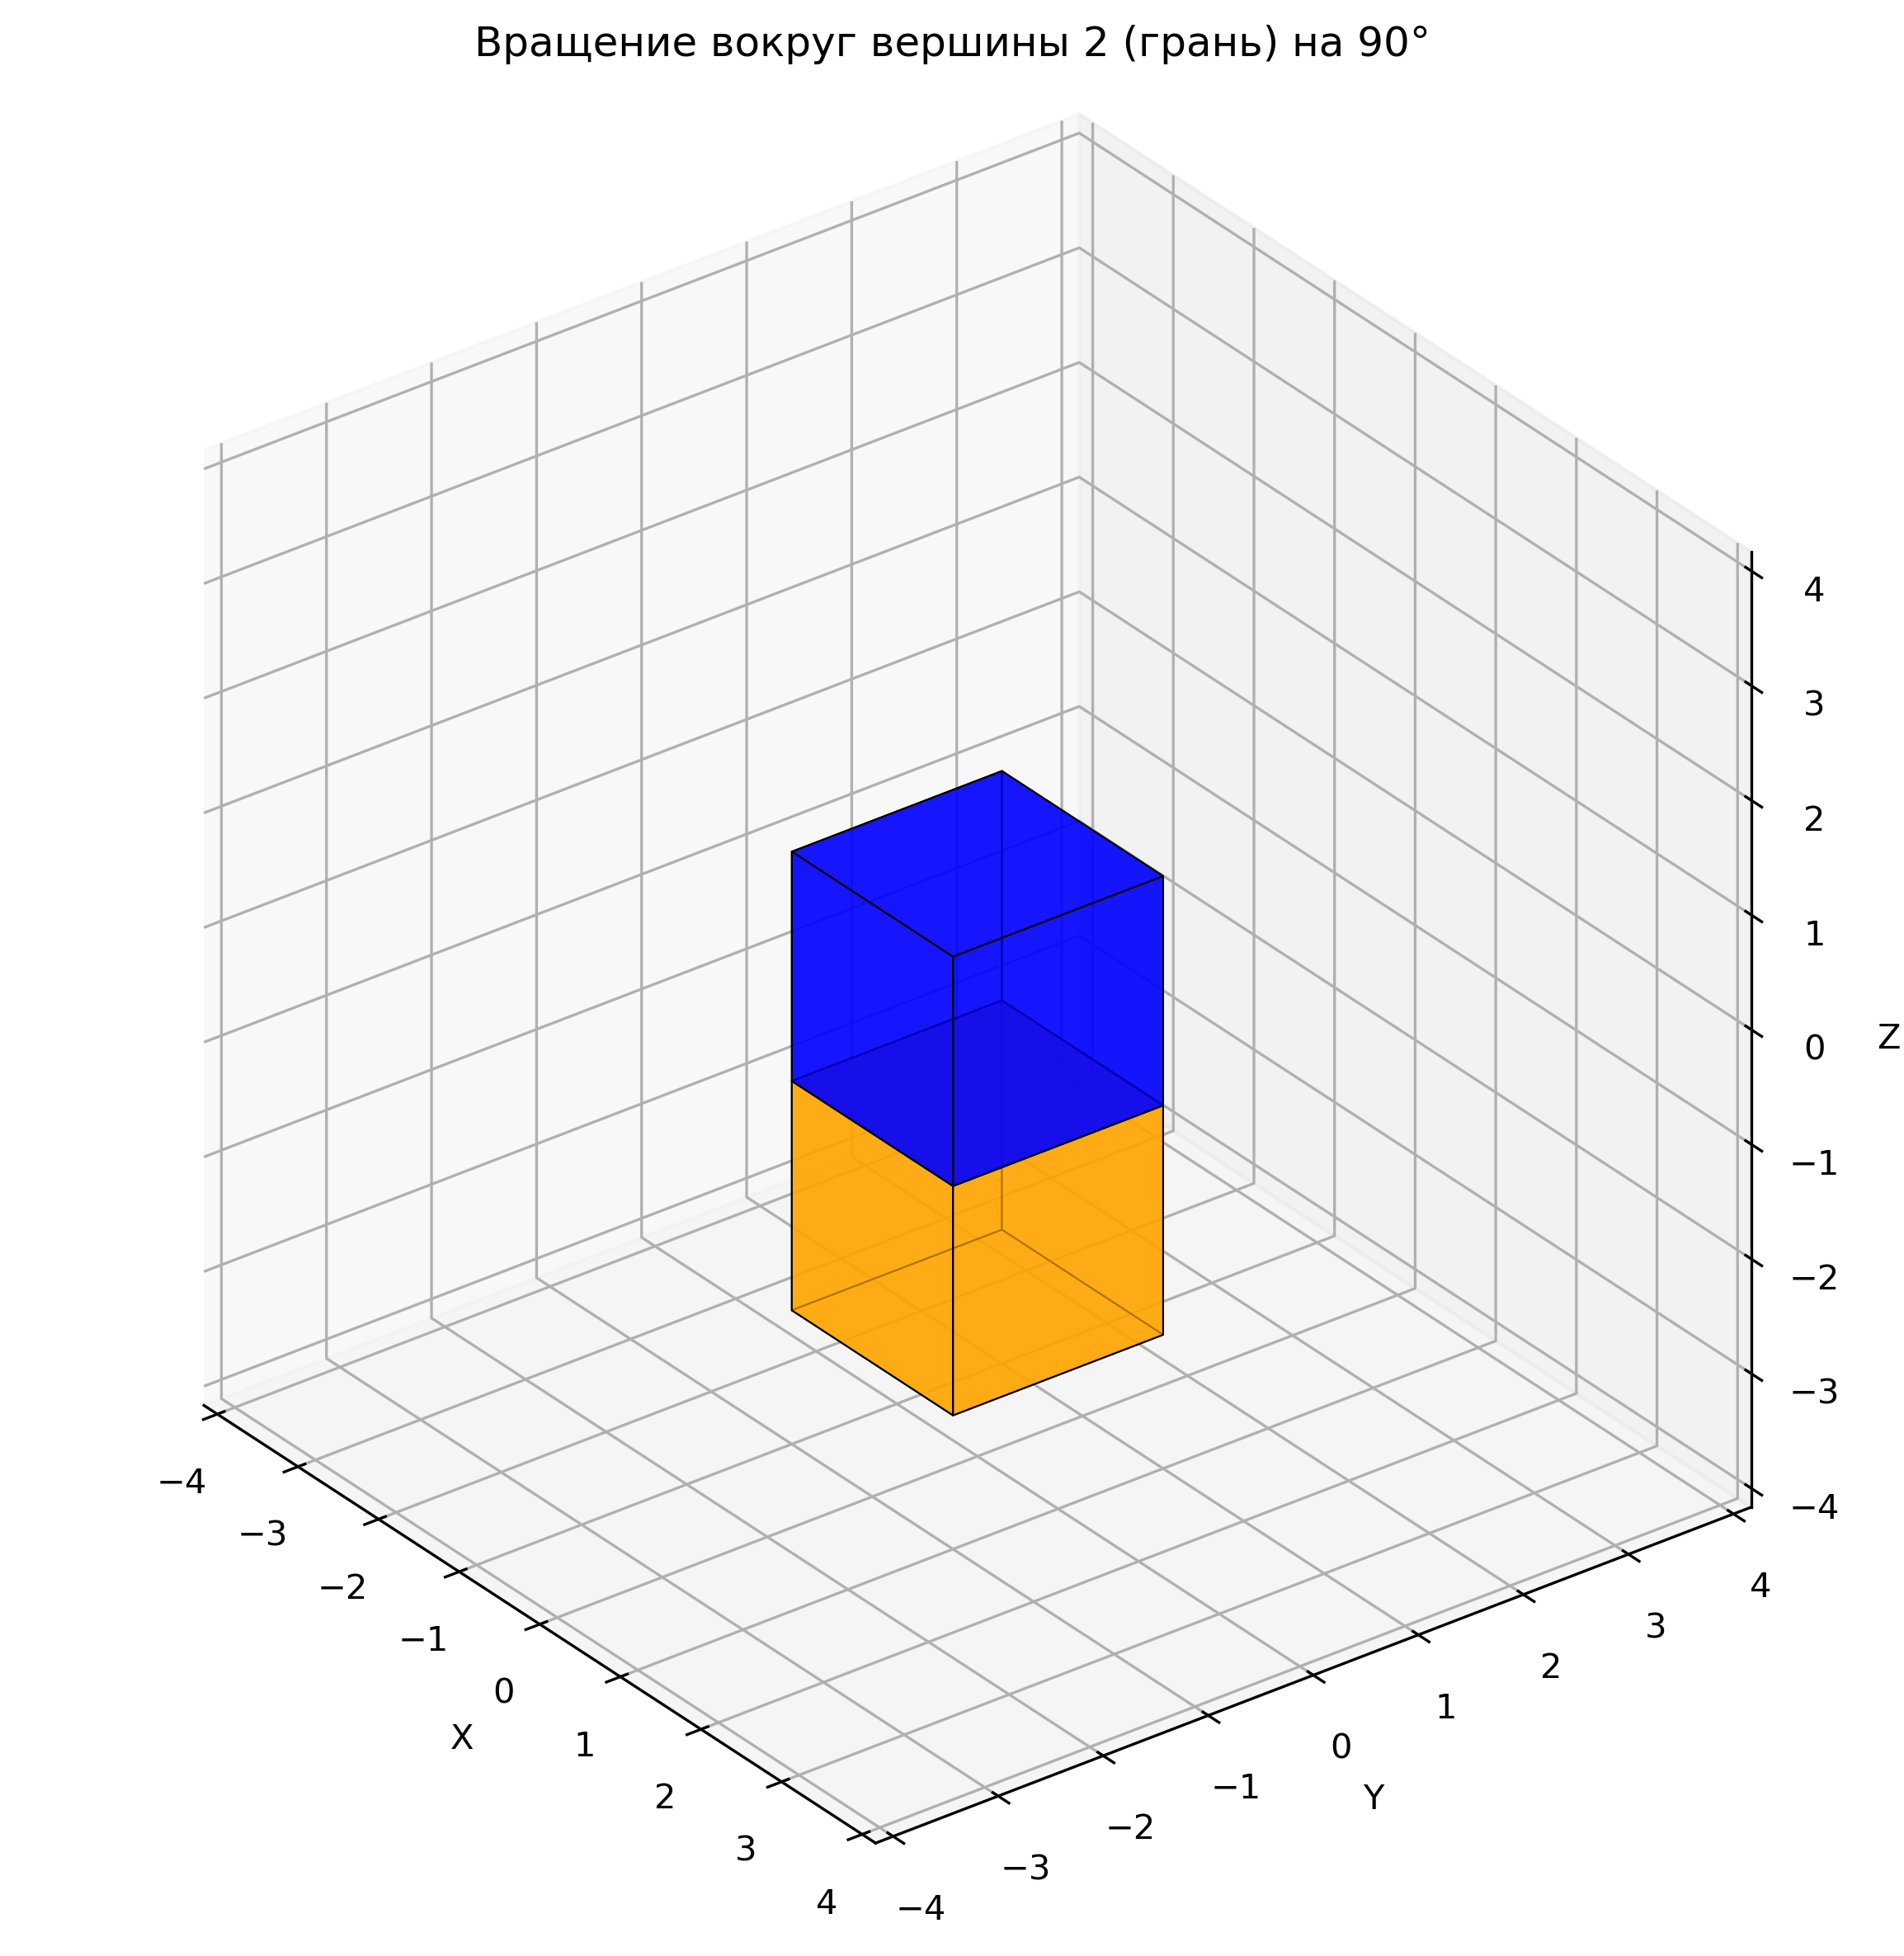
\includegraphics[width=0.8\textwidth]{images/task5/rotate_around_vertex_2.png}
\caption{Вращение вокруг вершины 2 (грань) на 90°}
\end{figure}

\begin{figure}[H]
\centering
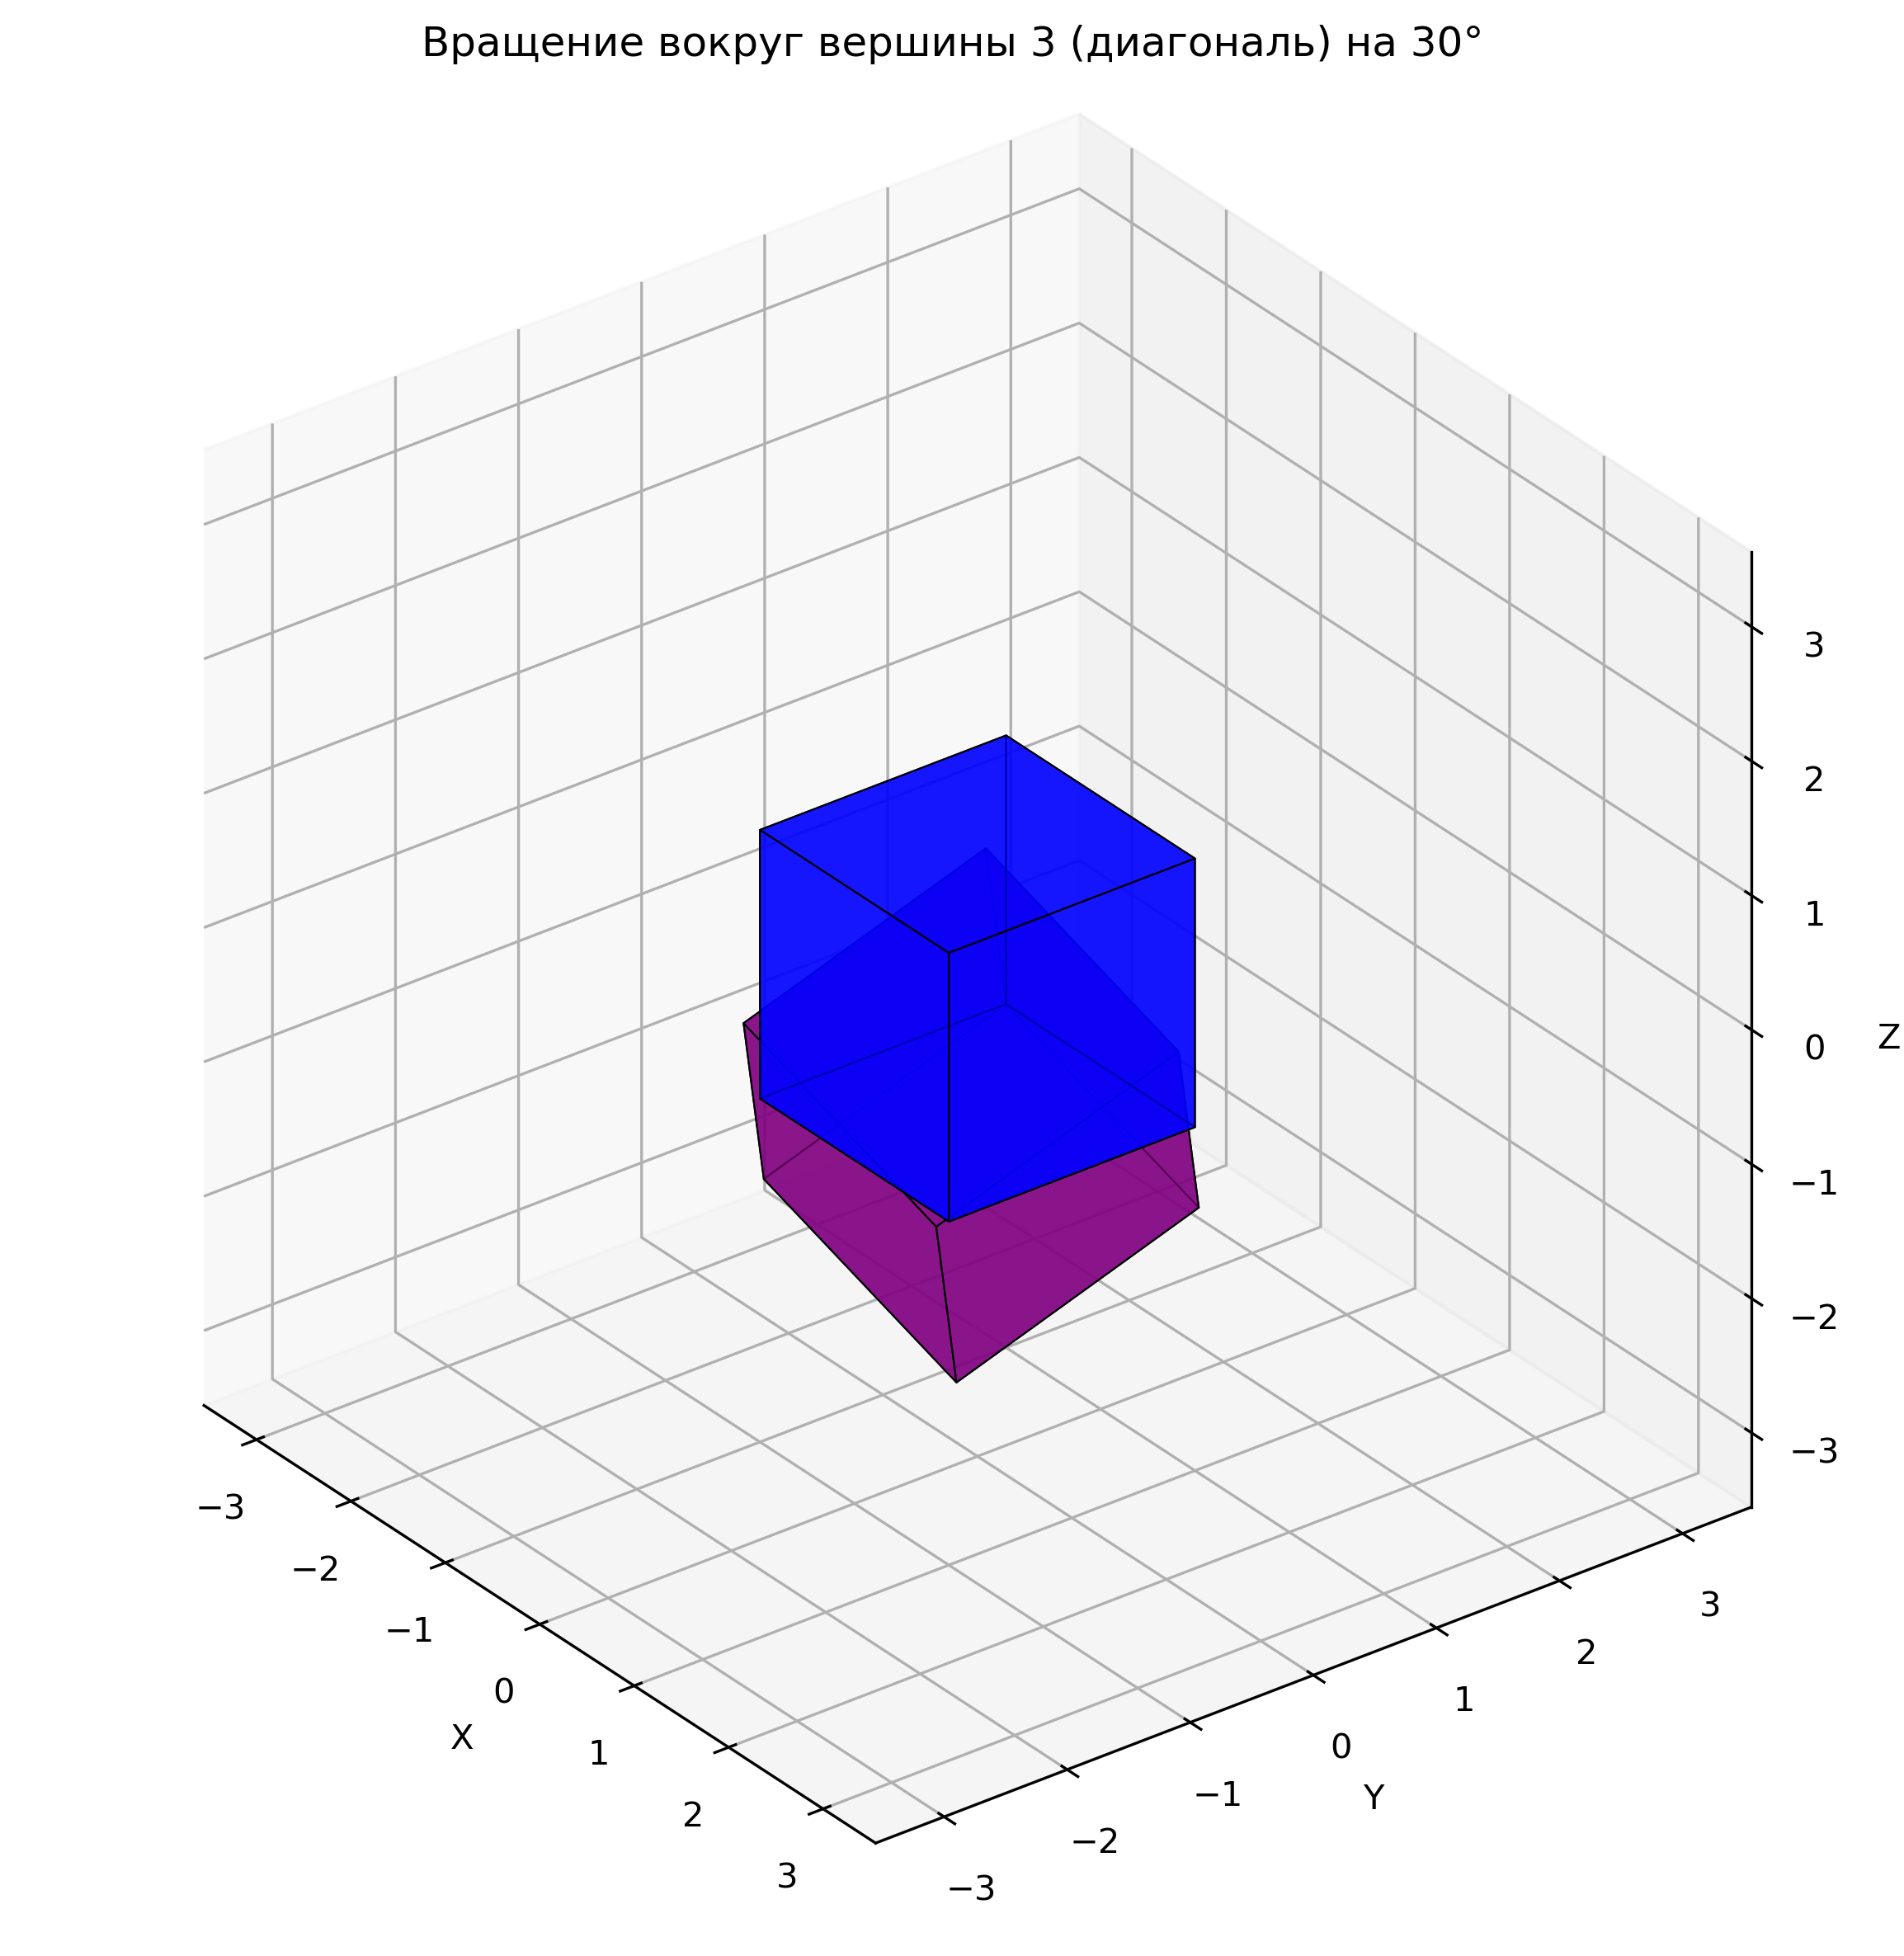
\includegraphics[width=0.8\textwidth]{images/task5/rotate_around_vertex_3.png}
\caption{Вращение вокруг вершины 3 (диагональ) на 30°}
\end{figure}

\begin{figure}[H]
\centering
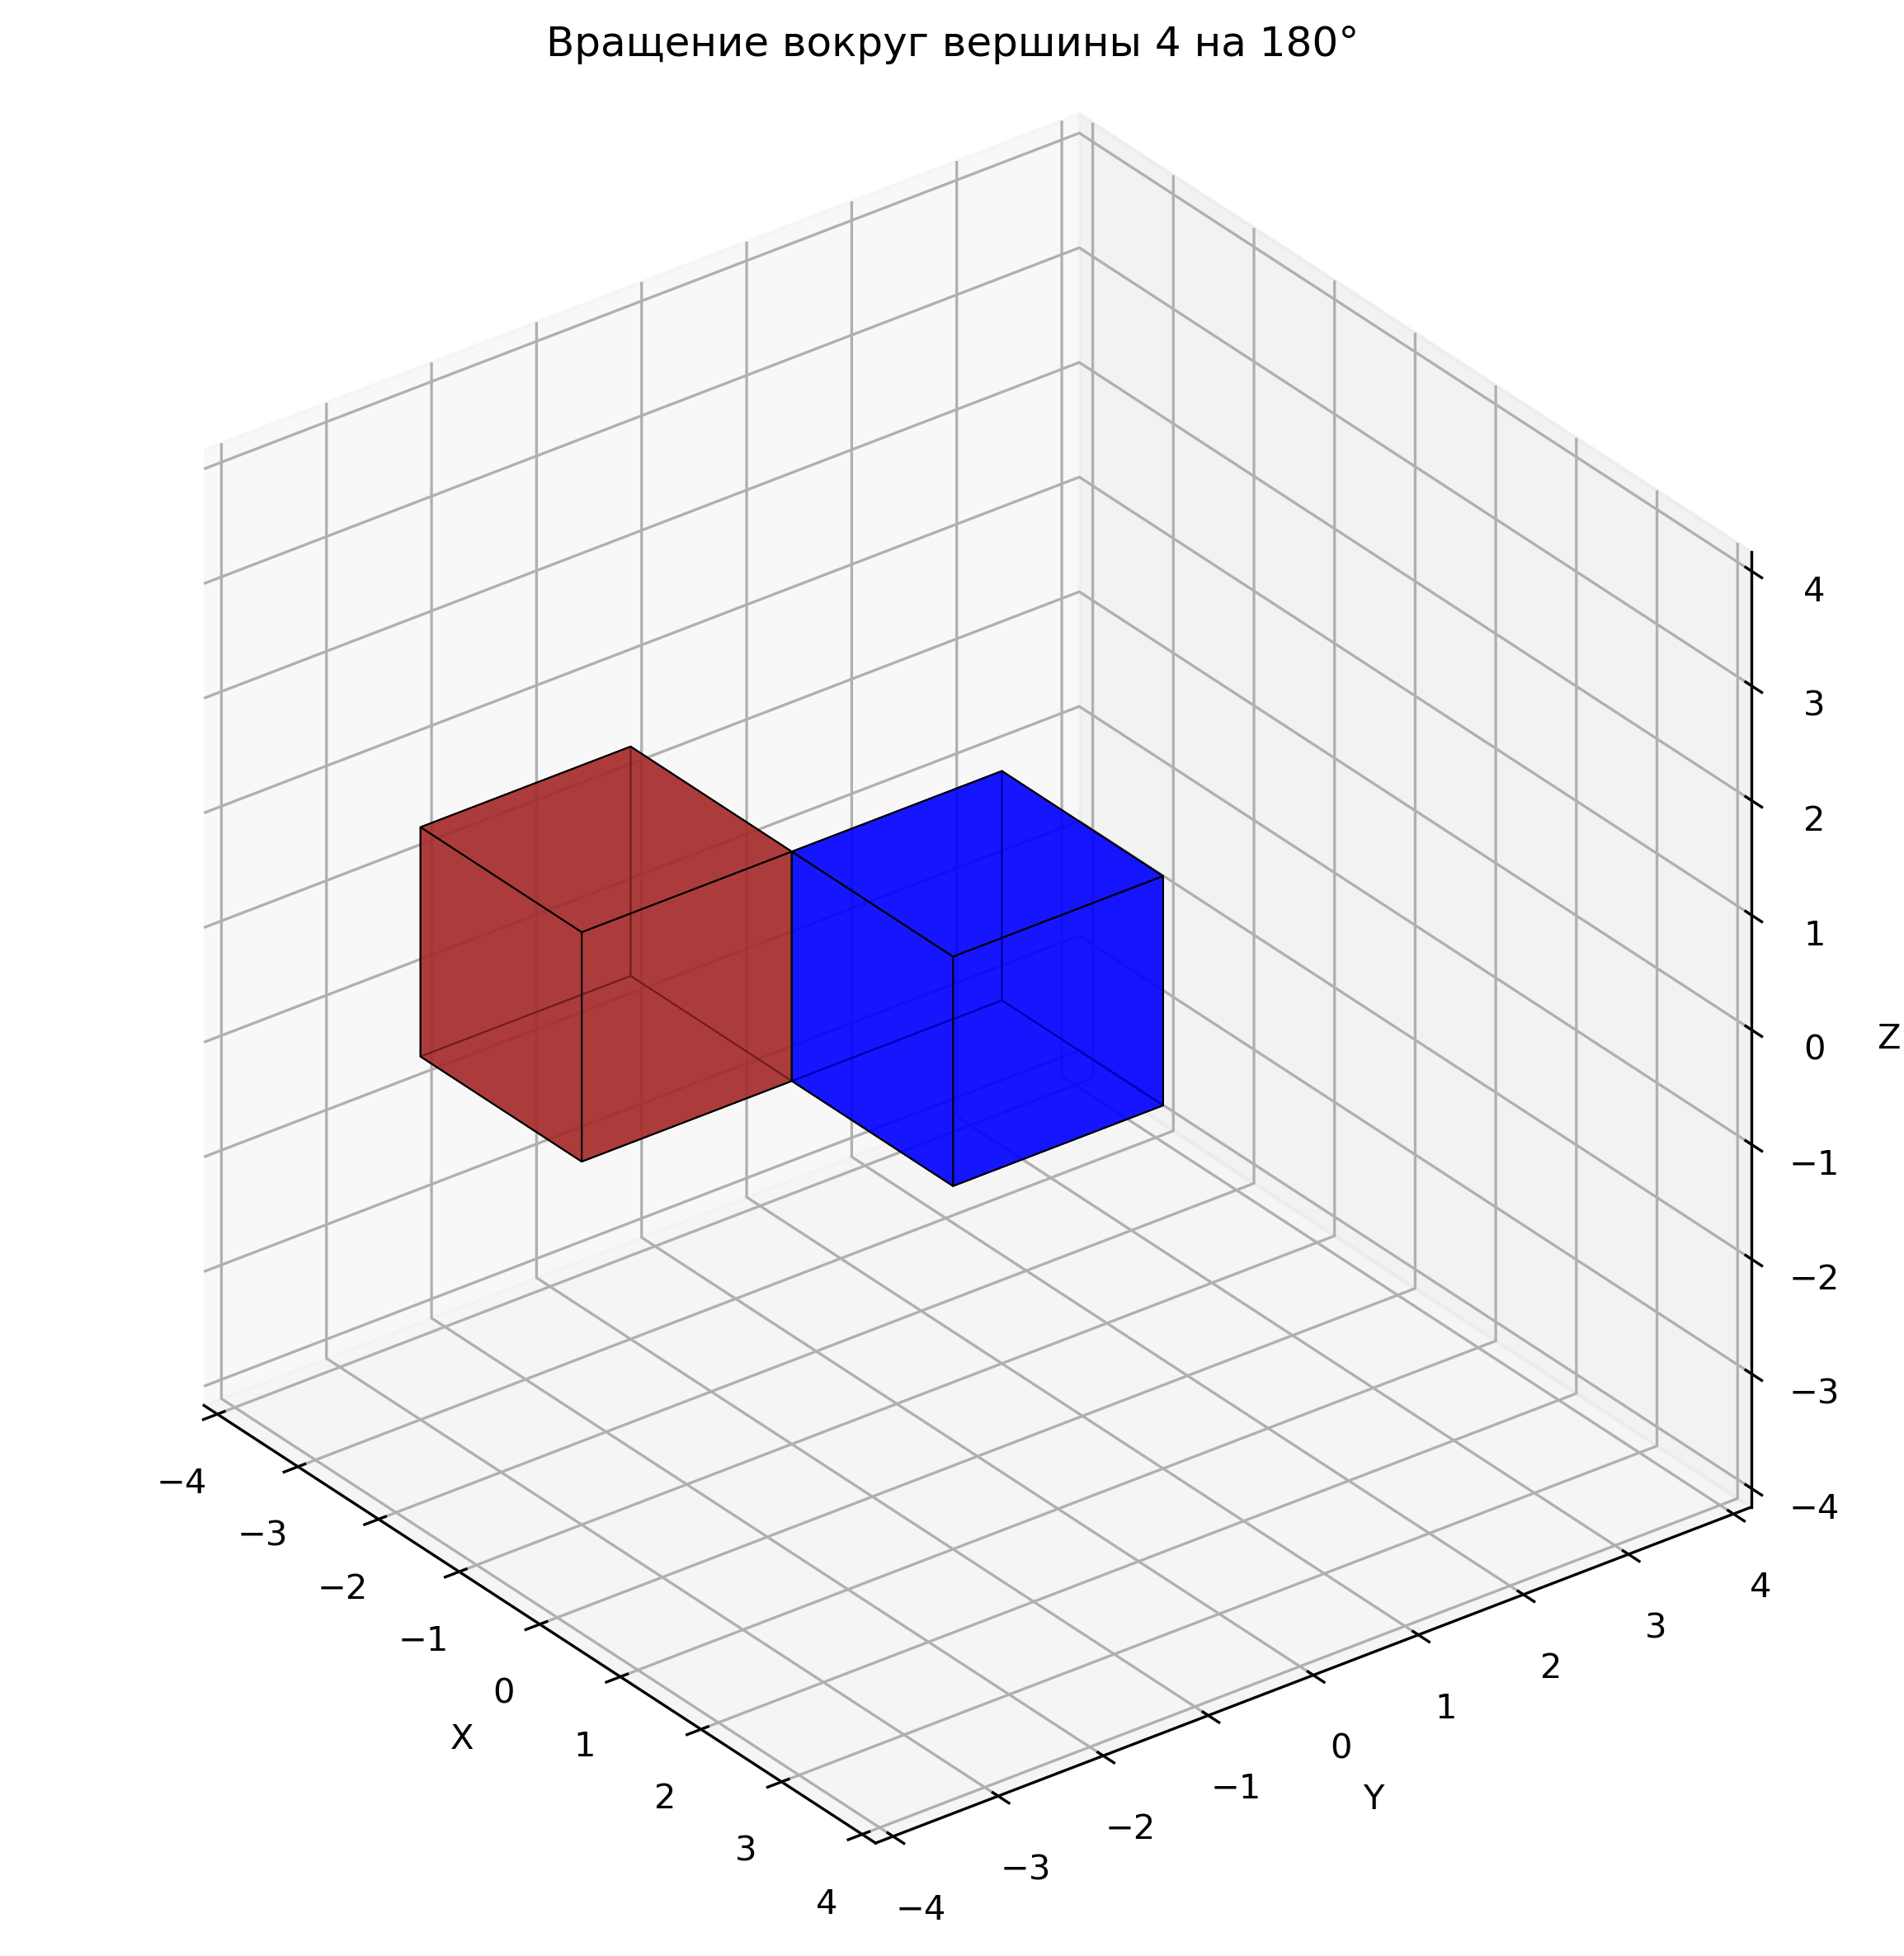
\includegraphics[width=0.8\textwidth]{images/task5/rotate_around_vertex_4.png}
\caption{Вращение вокруг вершины 4 на 180°}
\end{figure}

\begin{figure}[H]
\centering
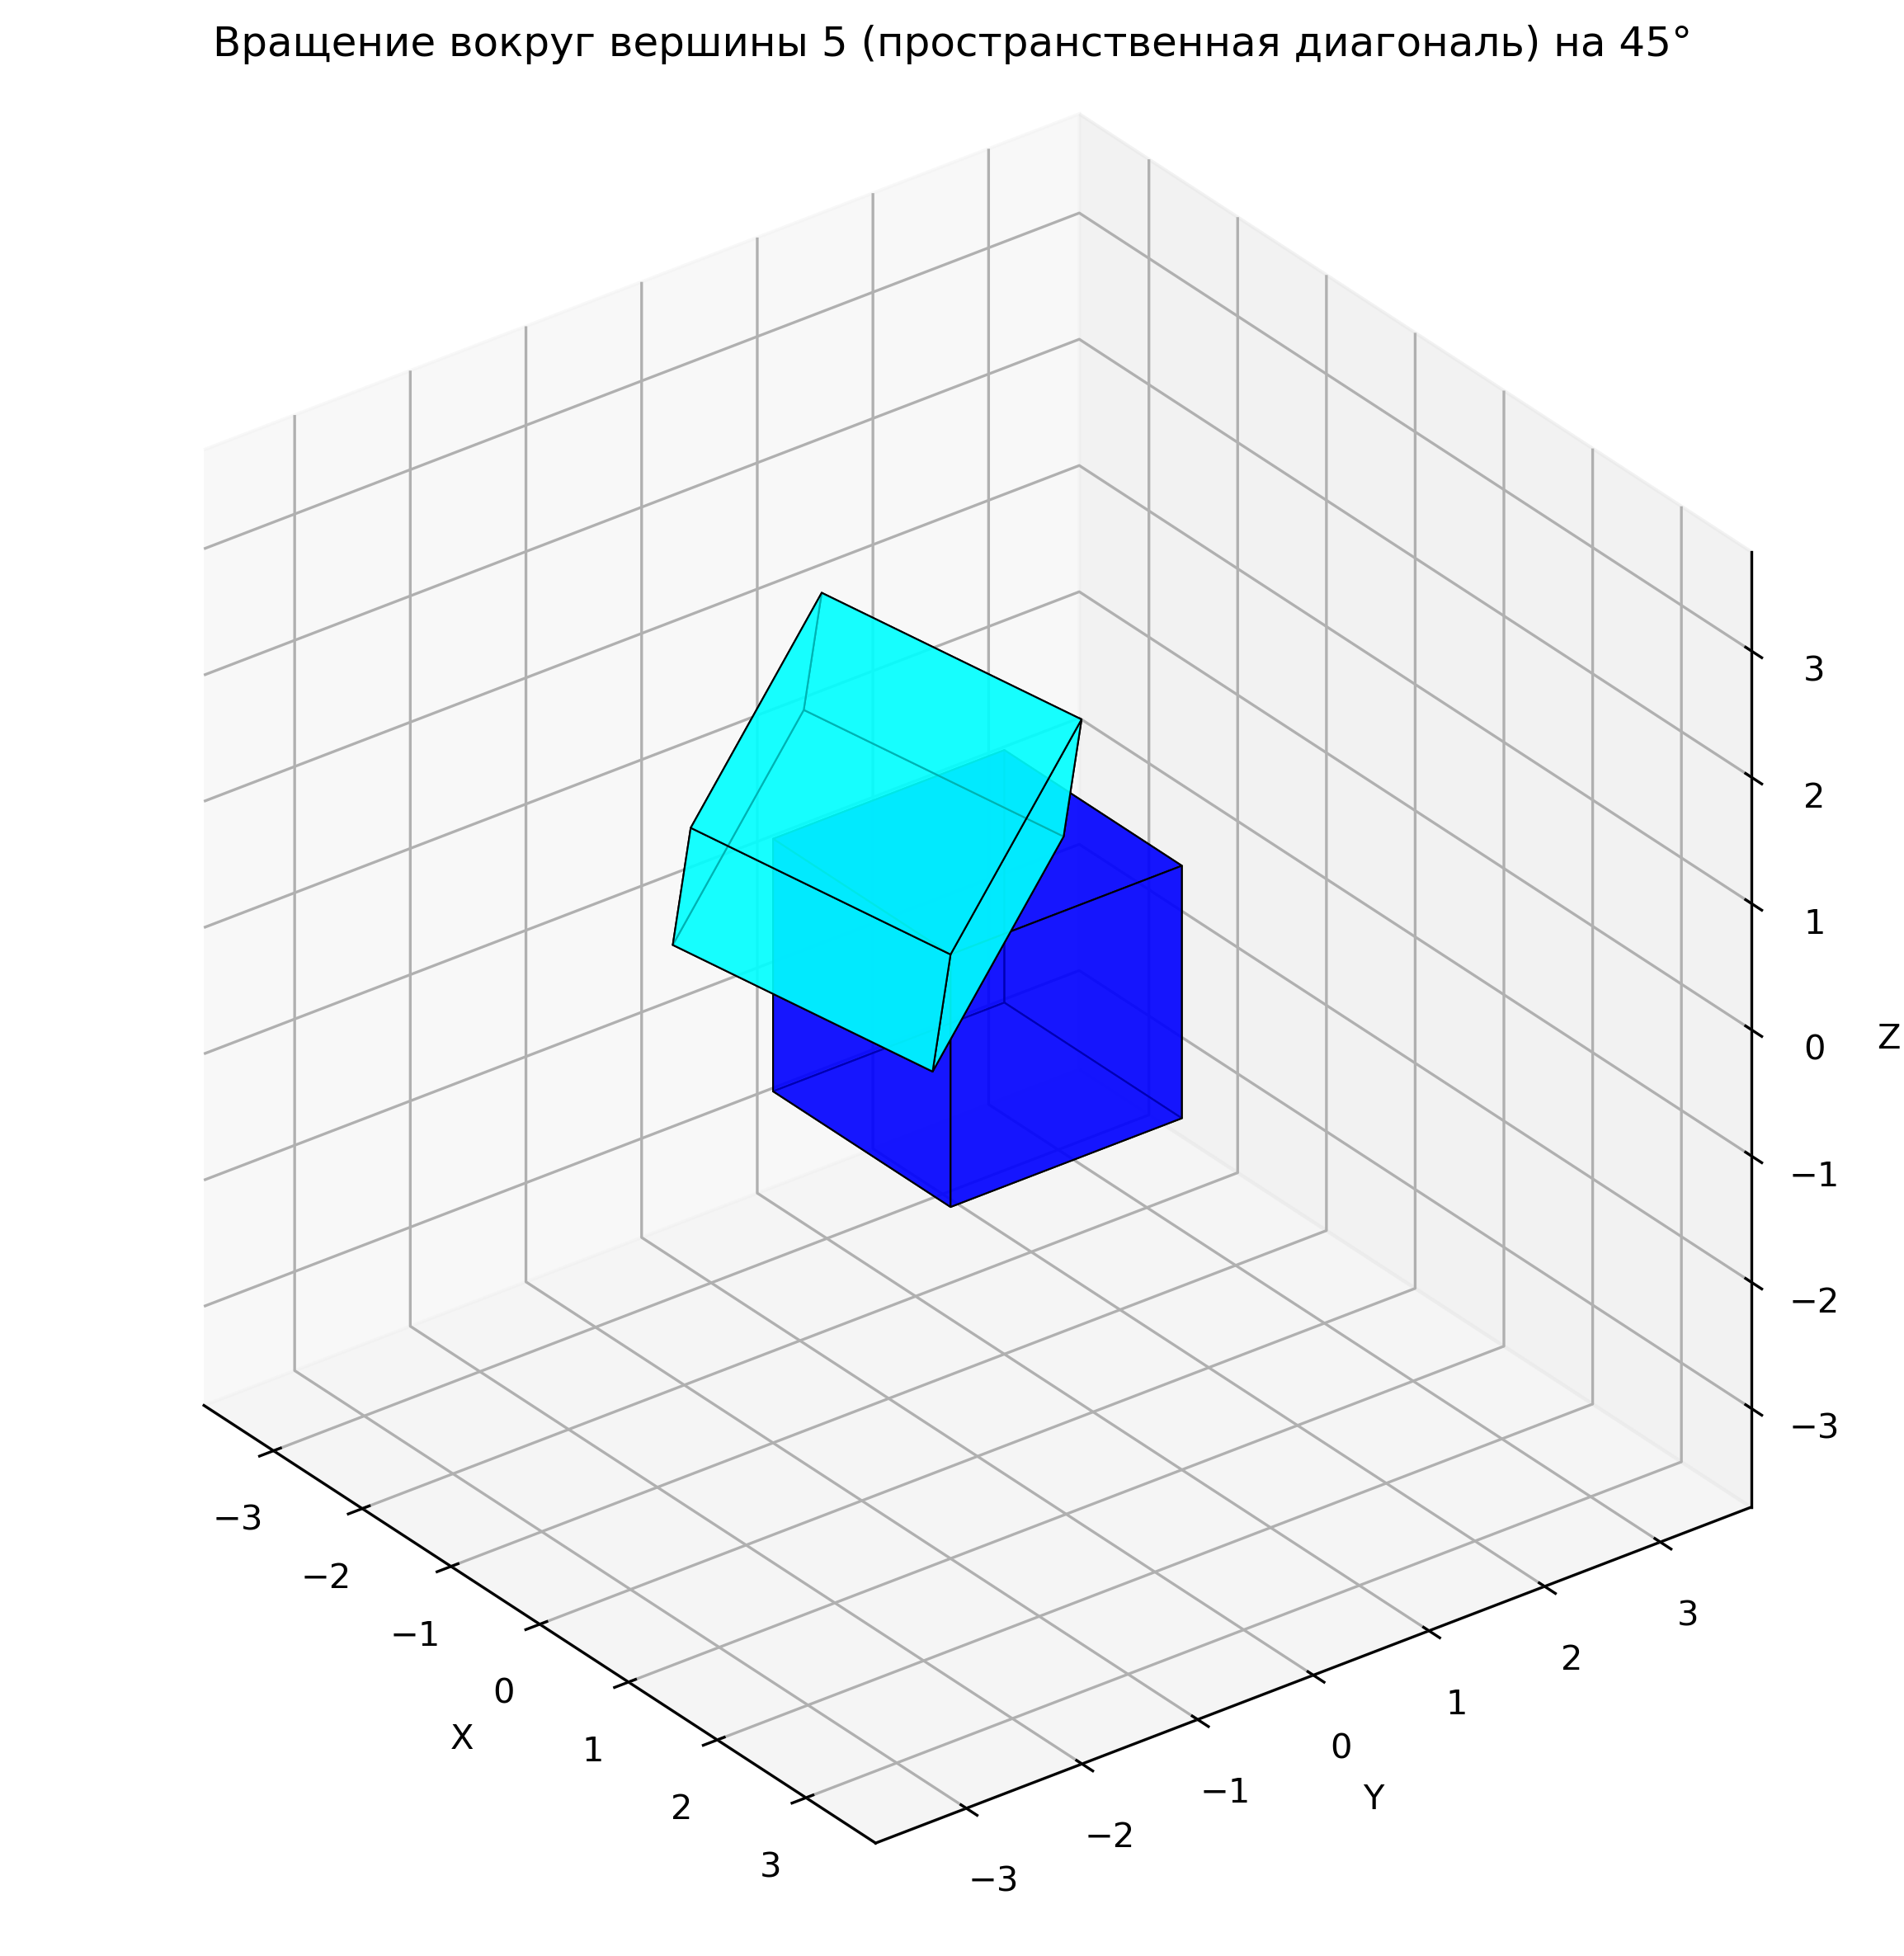
\includegraphics[width=0.8\textwidth]{images/task5/rotate_around_vertex_5.png}
\caption{Вращение вокруг вершины 5 (пространственная диагональ) на 45°}
\end{figure}

\subsection*{Анализ свойств}
\begin{itemize}
    \item Выбранная вершина остается неподвижной
    \item Объем и форма кубика сохраняются
    \item Центр кубика может смещаться
    \item Преобразование не является ортогональным в целом
\end{itemize}

\section*{Задание 6: Реализация камеры}

\subsection*{Постановка задачи}
Реализовать камеру с возможностью изменения позиции и ориентации, а также исследовать обратное преобразование камеры.

\subsection*{Математические основы}
Матрица камеры состоит из двух частей:
\begin{enumerate}
    \item Матрица поворота камеры $R_{camera}$
    \item Матрица перемещения камеры $T_{camera}$
\end{enumerate}

Полная матрица камеры: $C = R_{camera} \cdot T_{camera}$

\subsection*{Результаты}
Исследованы различные позиции камеры:

\begin{figure}[H]
\centering
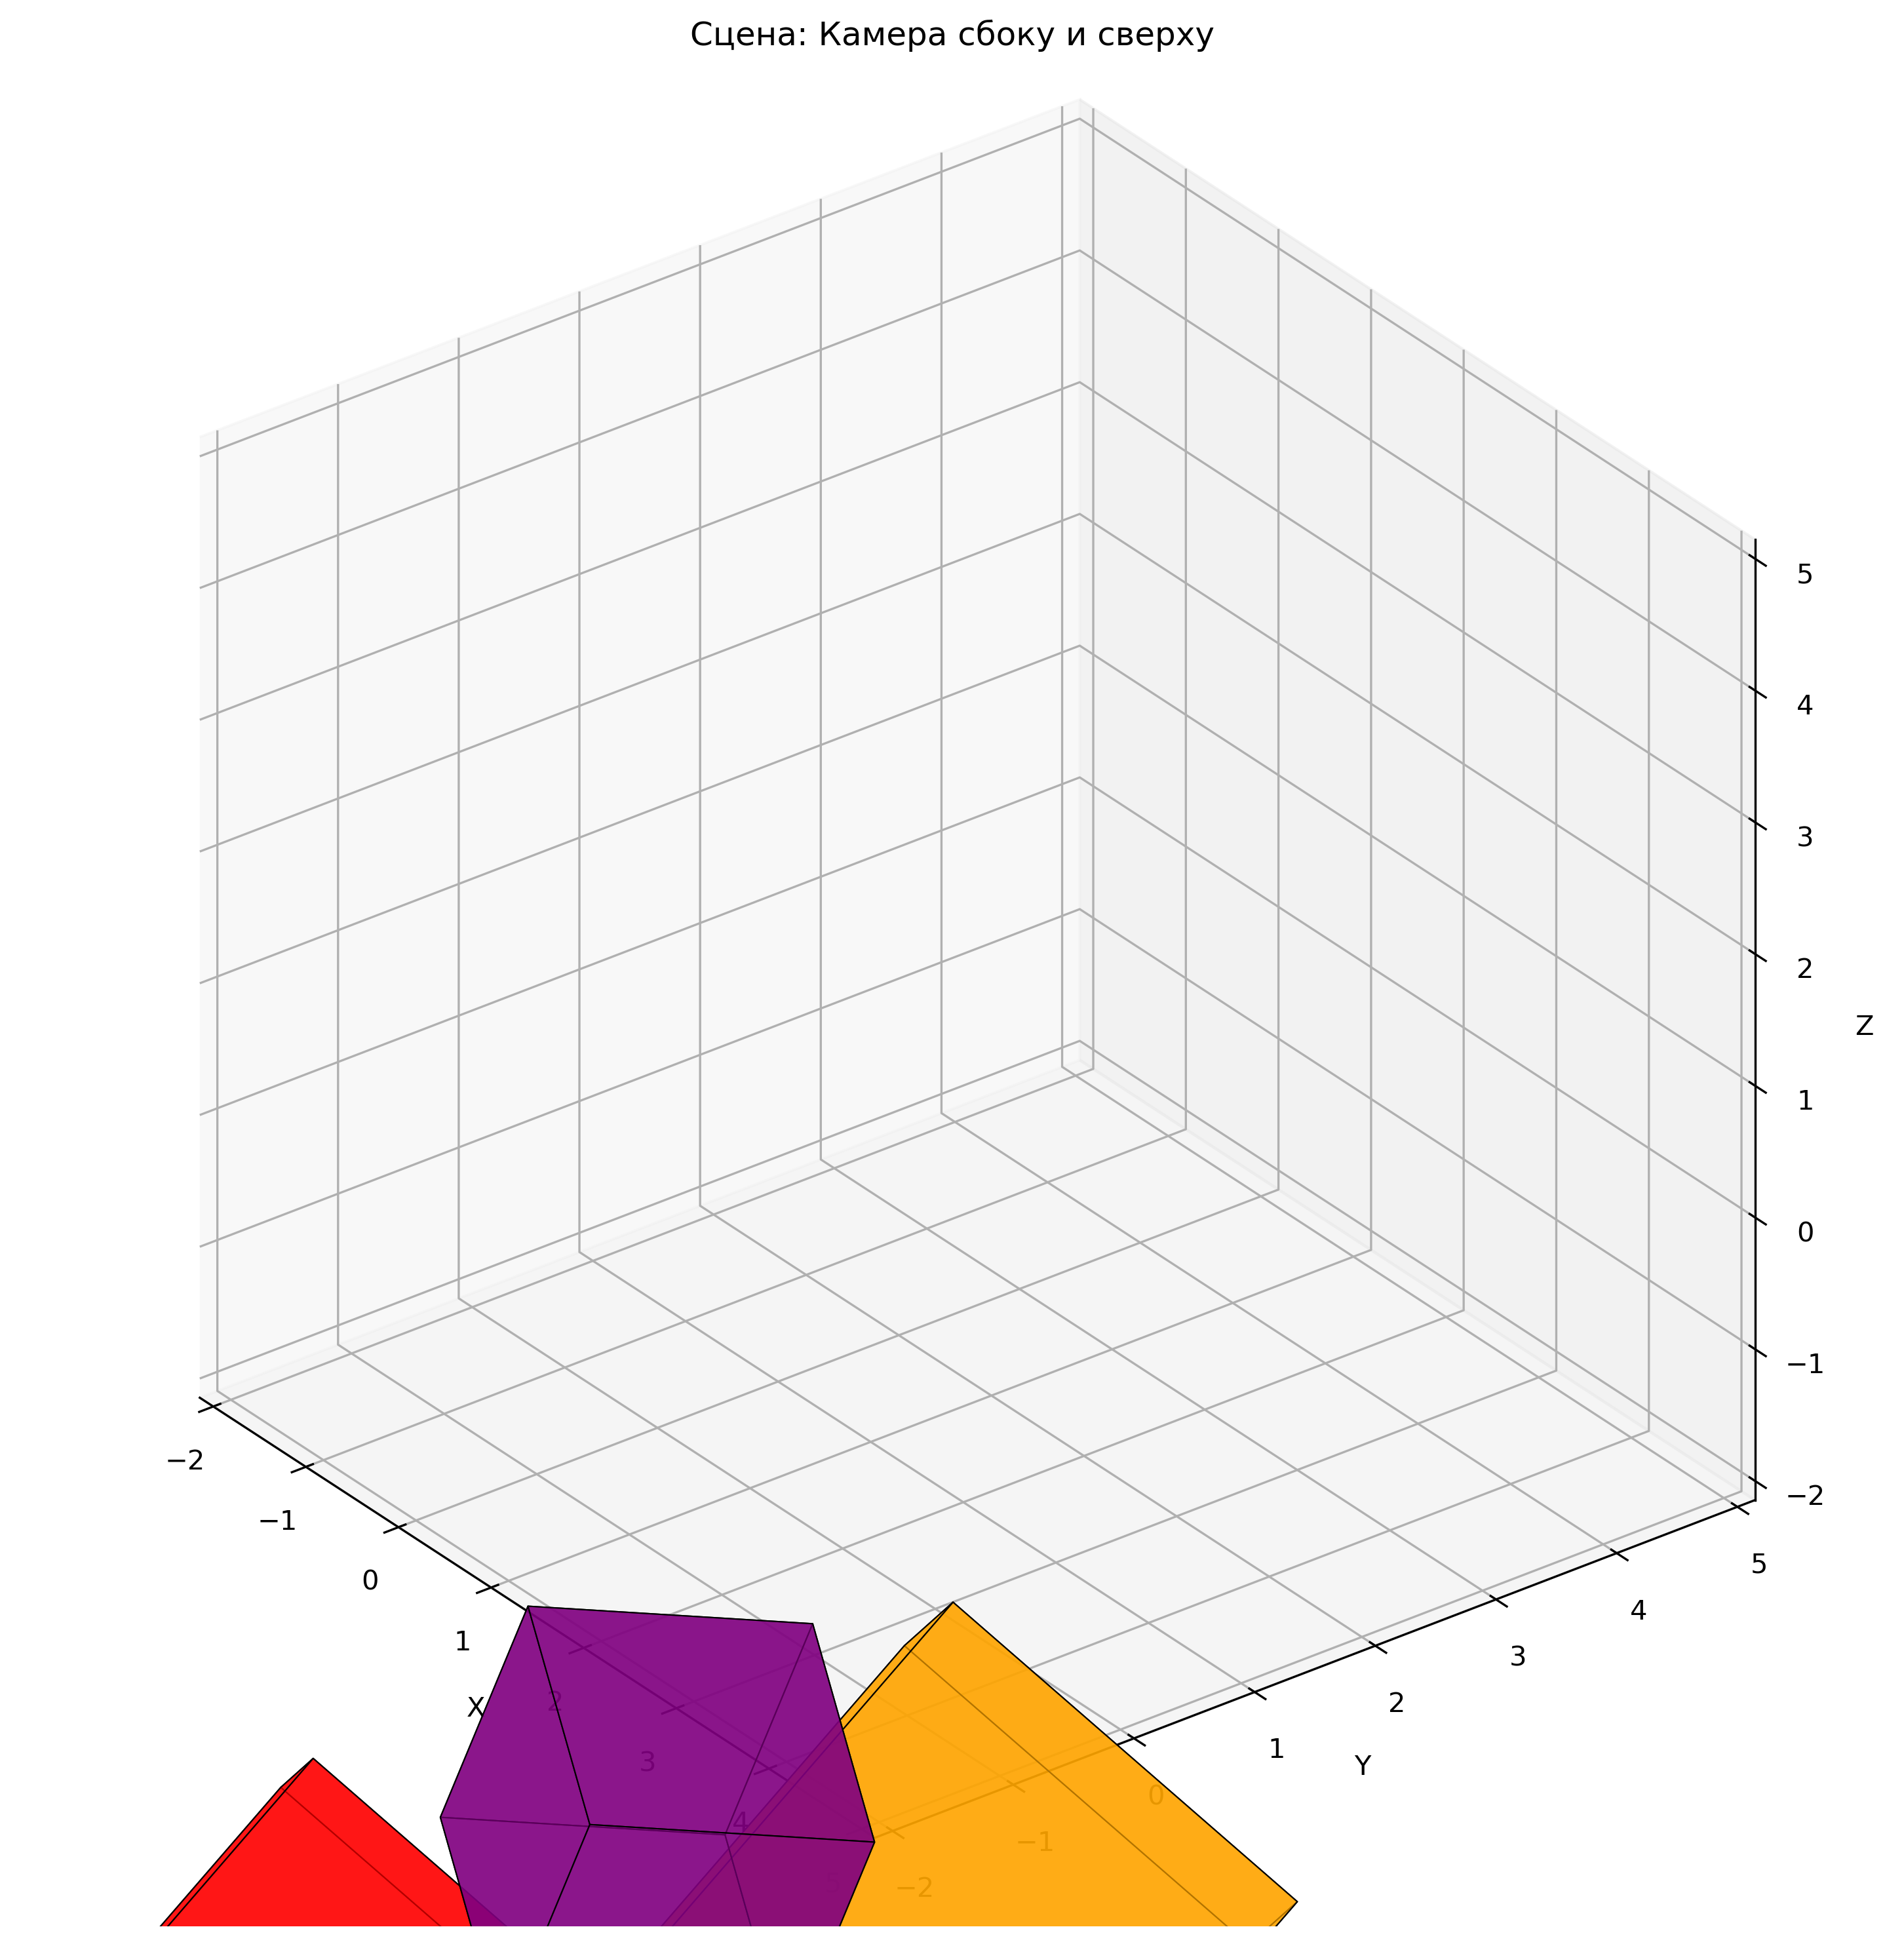
\includegraphics[width=0.8\textwidth]{images/task6/camera_side_top.png}
\caption{Камера сбоку и сверху}
\end{figure}

\begin{figure}[H]
\centering
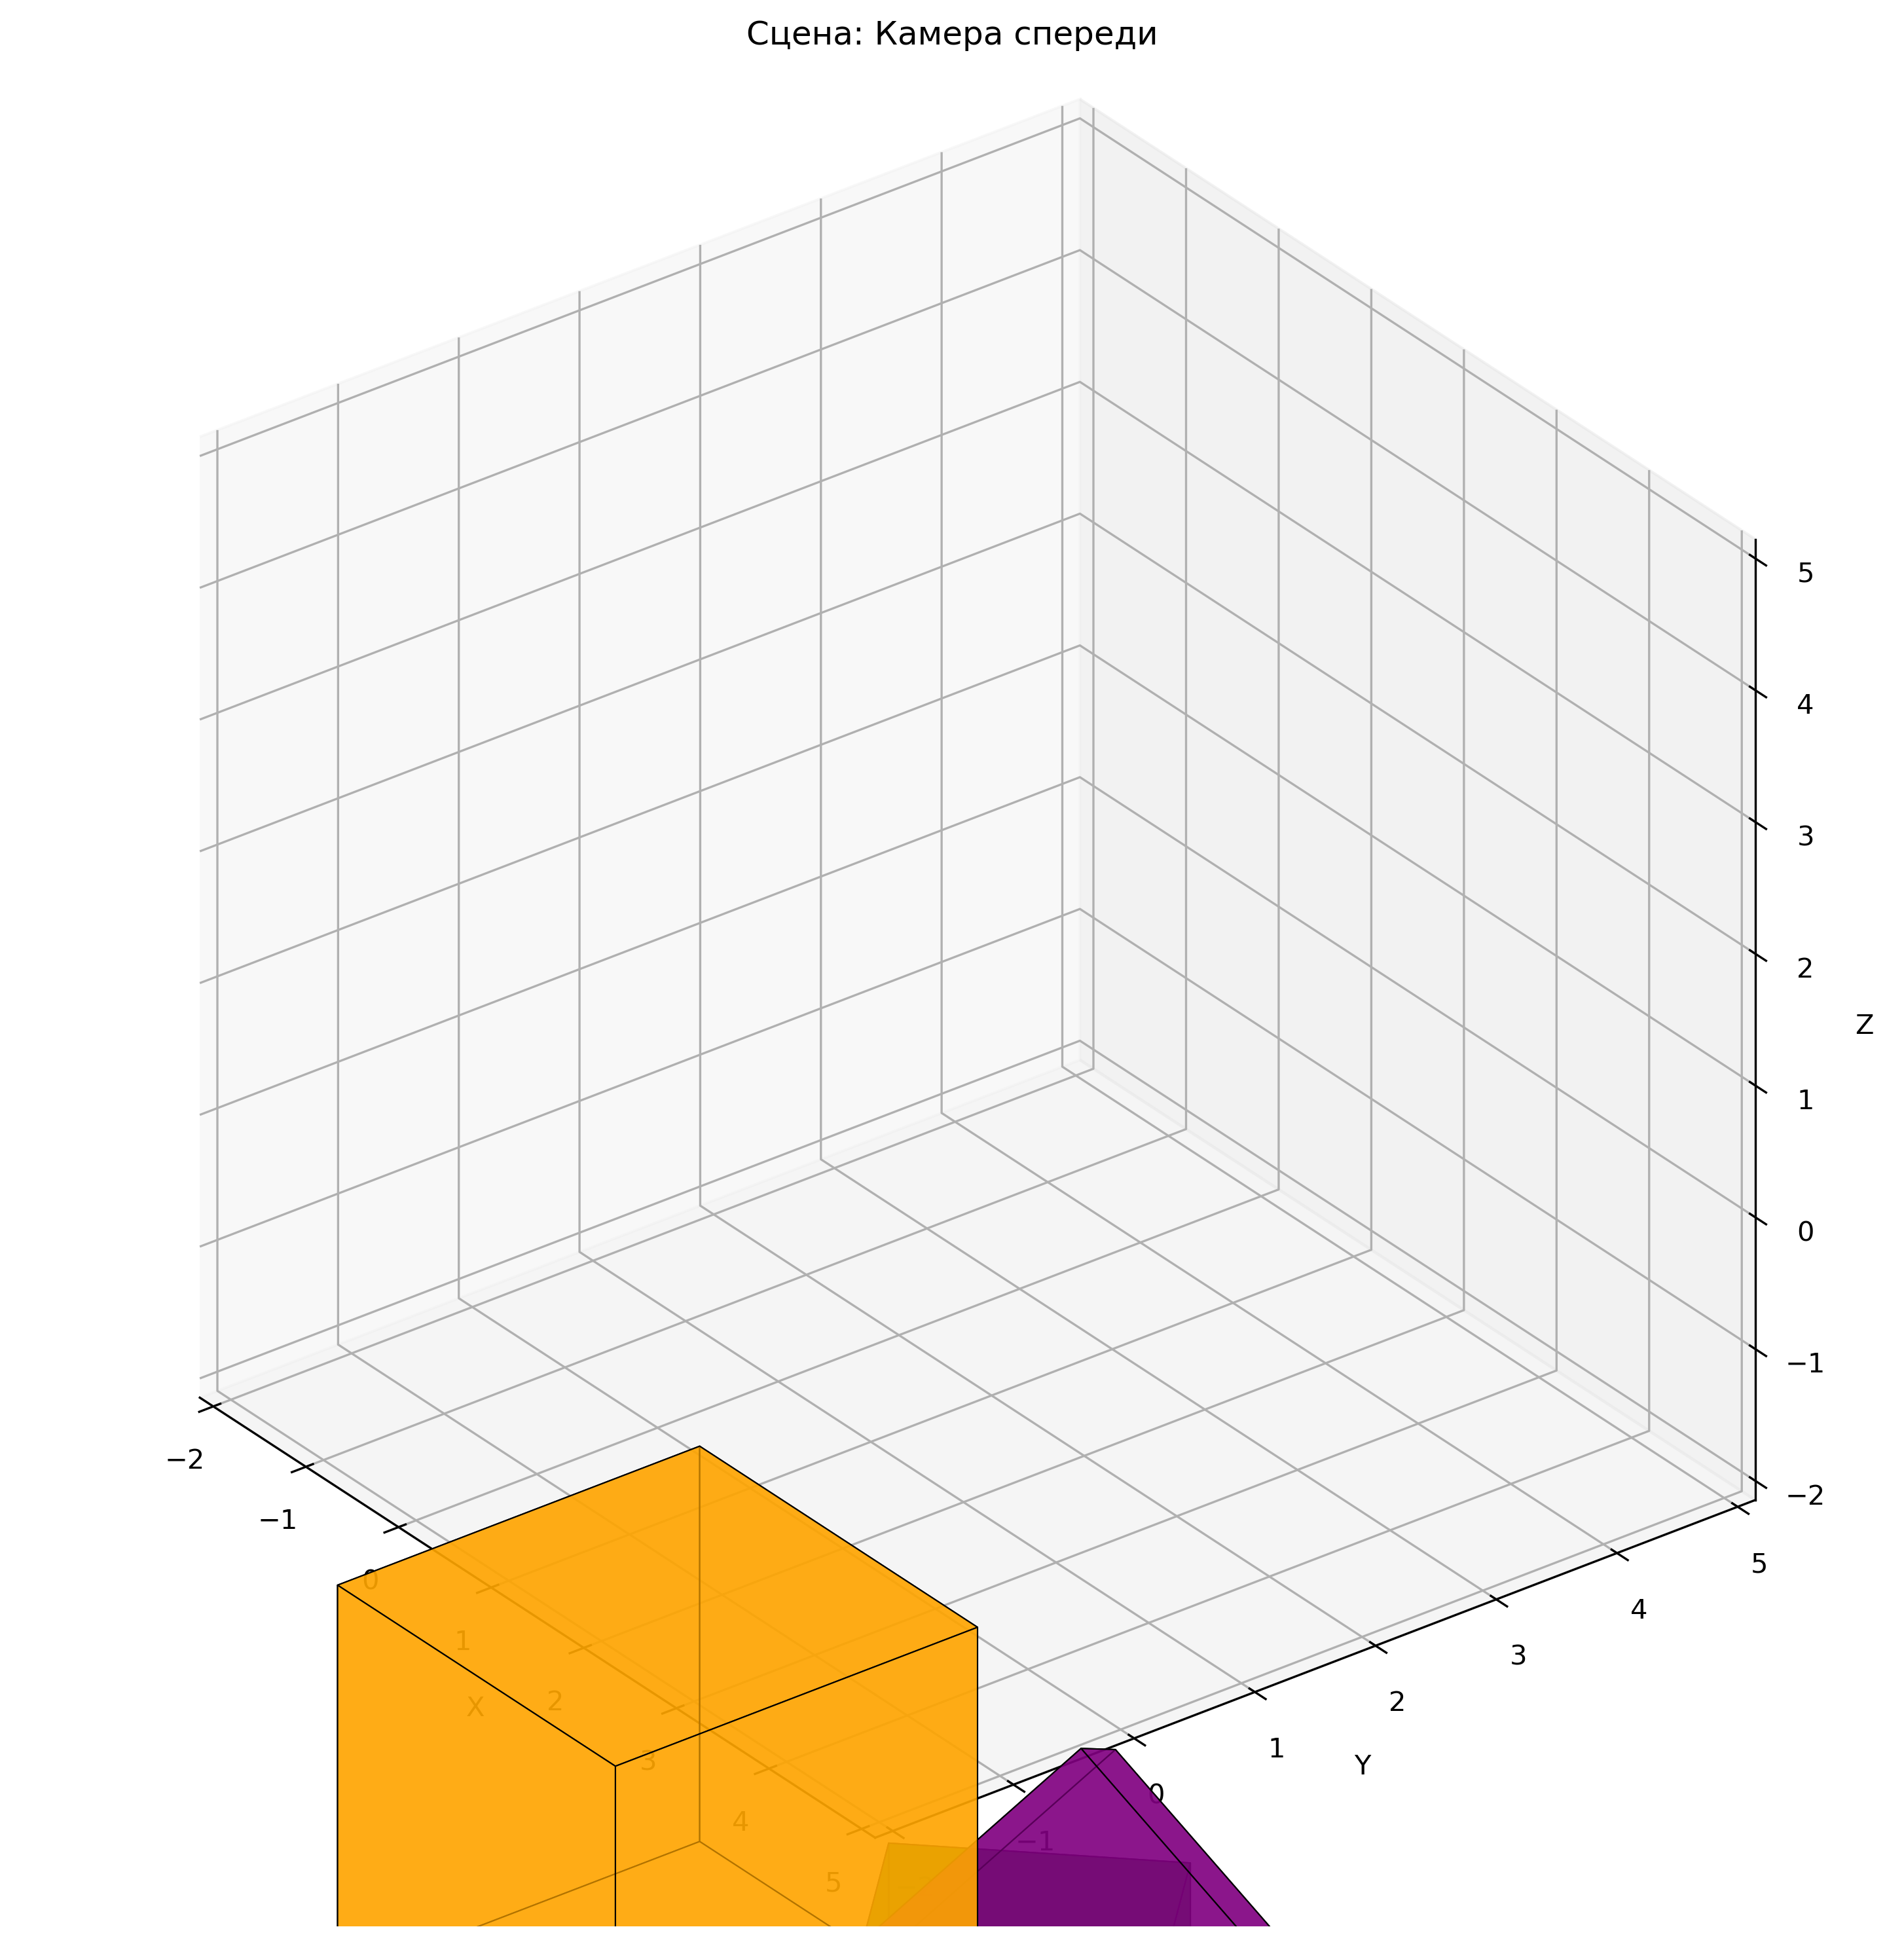
\includegraphics[width=0.8\textwidth]{images/task6/camera_front.png}
\caption{Камера спереди}
\end{figure}

\begin{figure}[H]
\centering
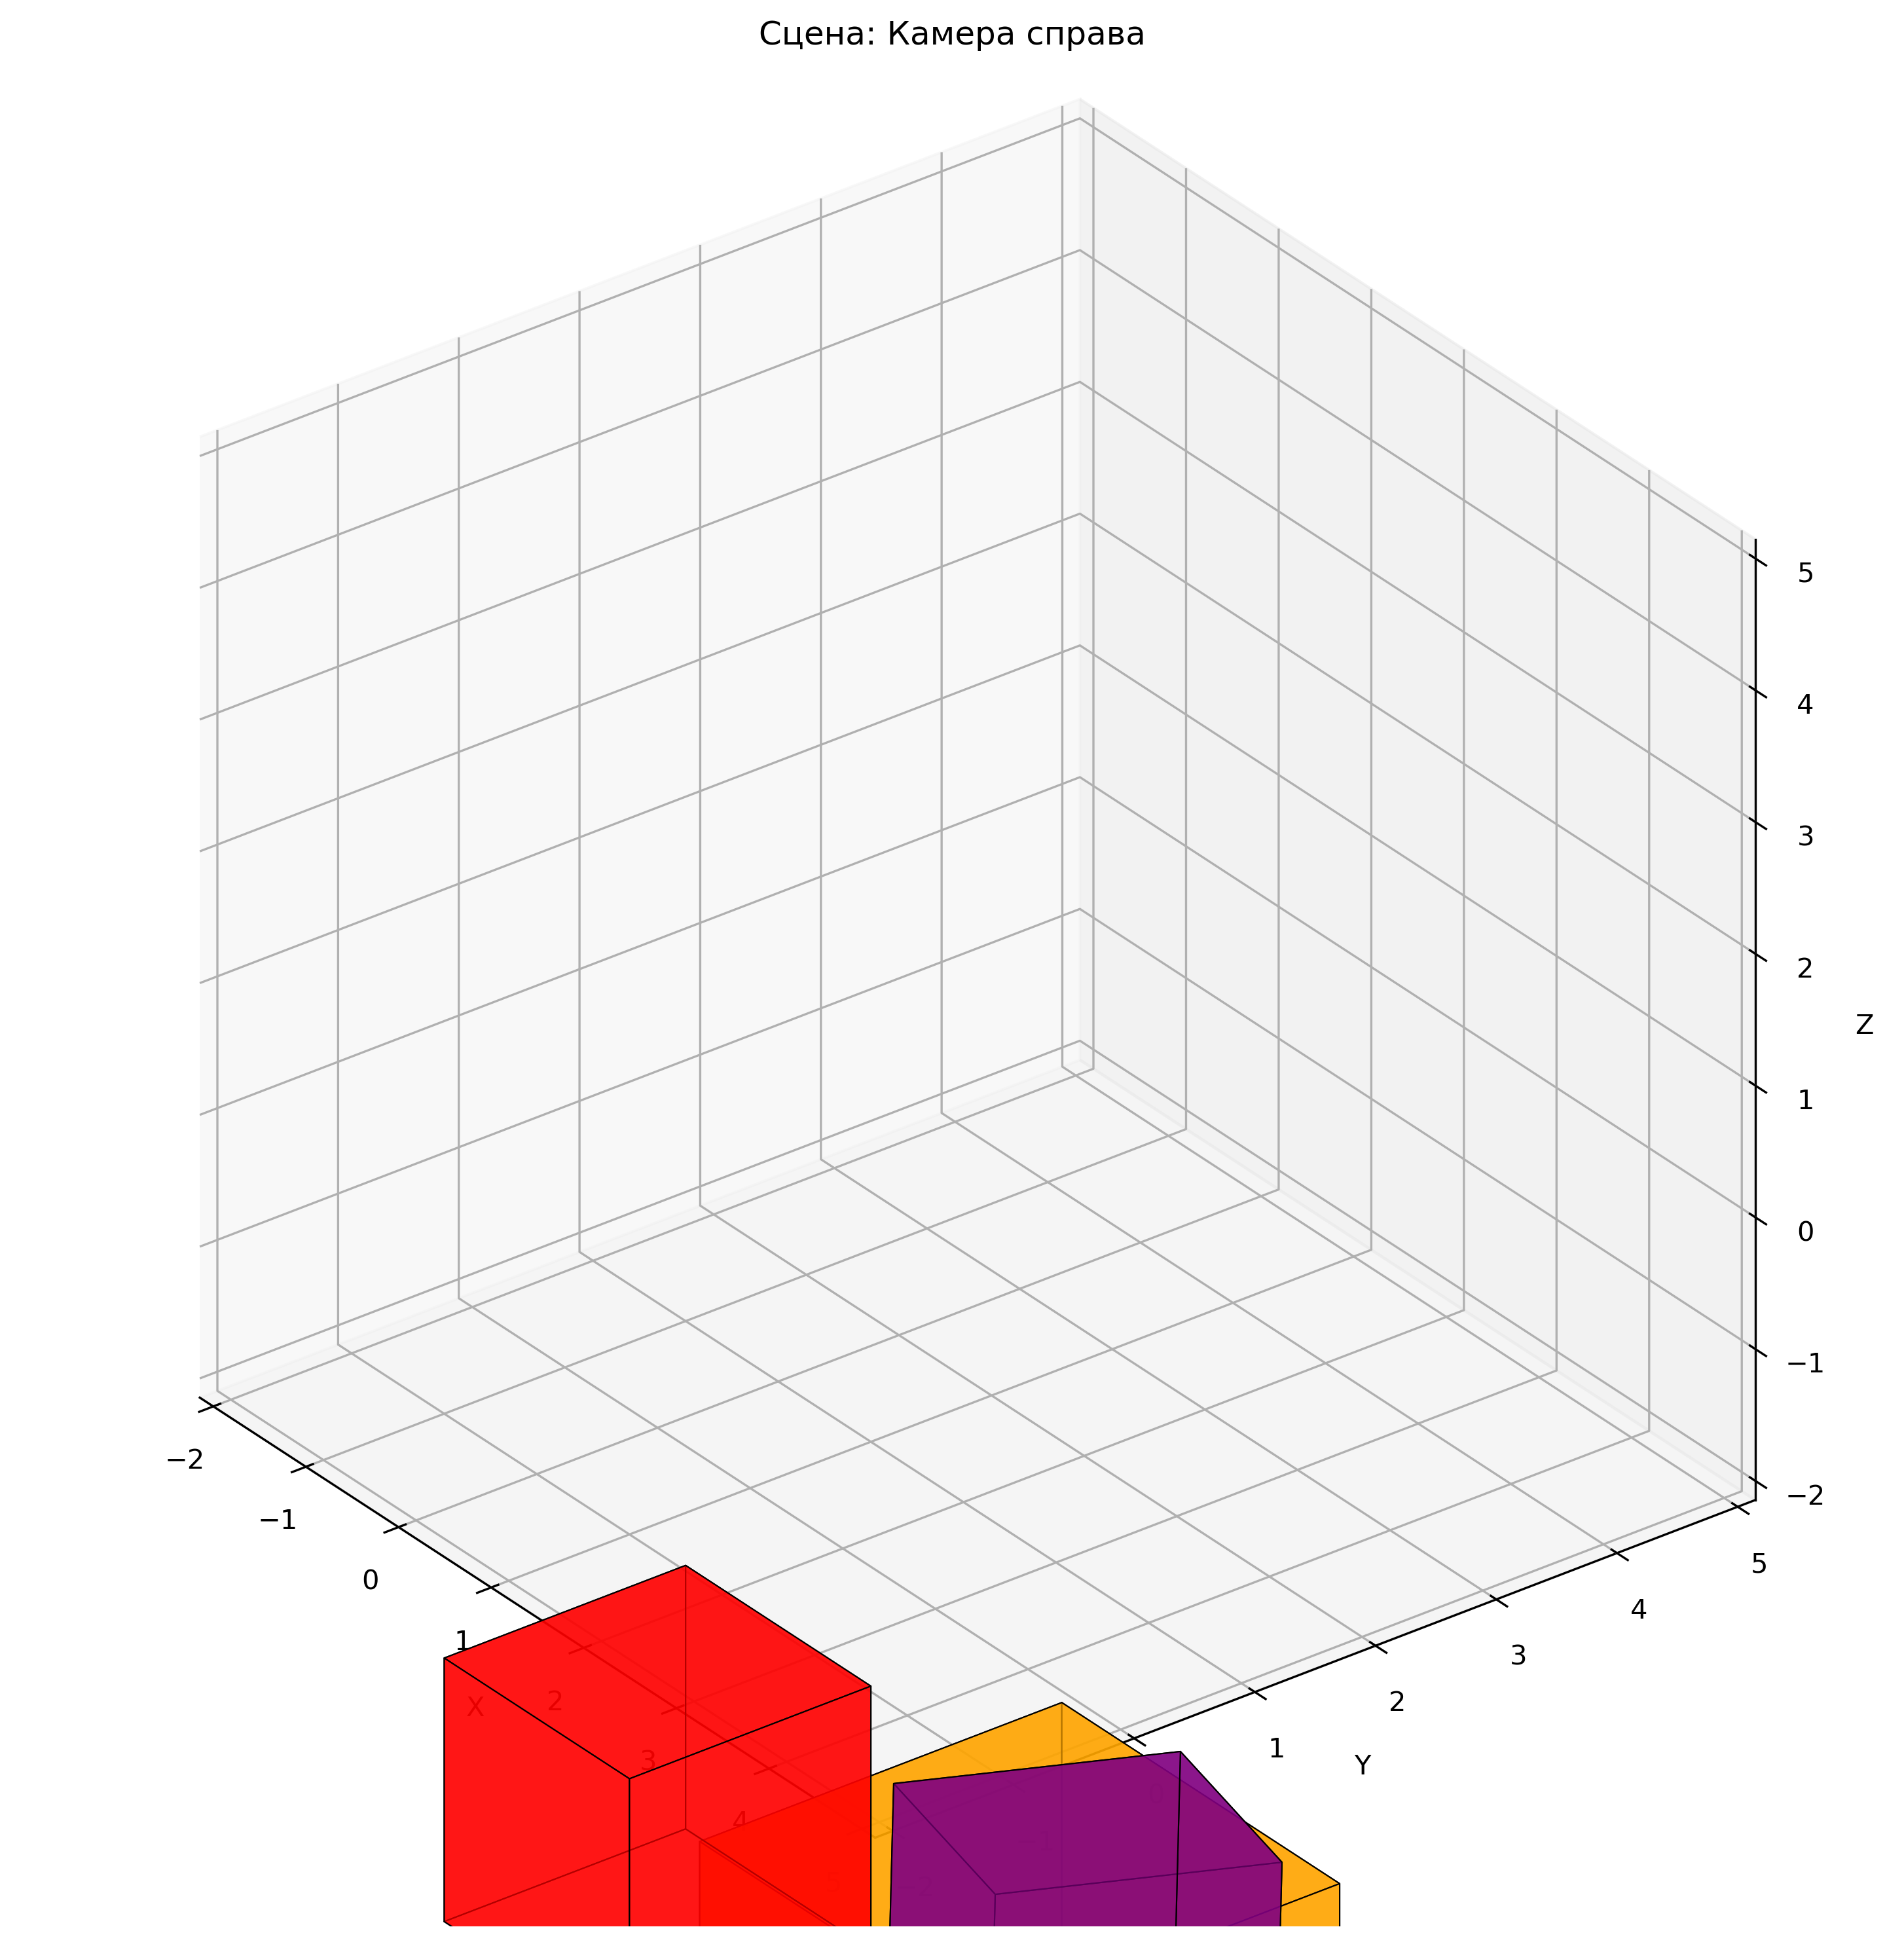
\includegraphics[width=0.8\textwidth]{images/task6/camera_right.png}
\caption{Камера справа}
\end{figure}

\begin{figure}[H]
\centering
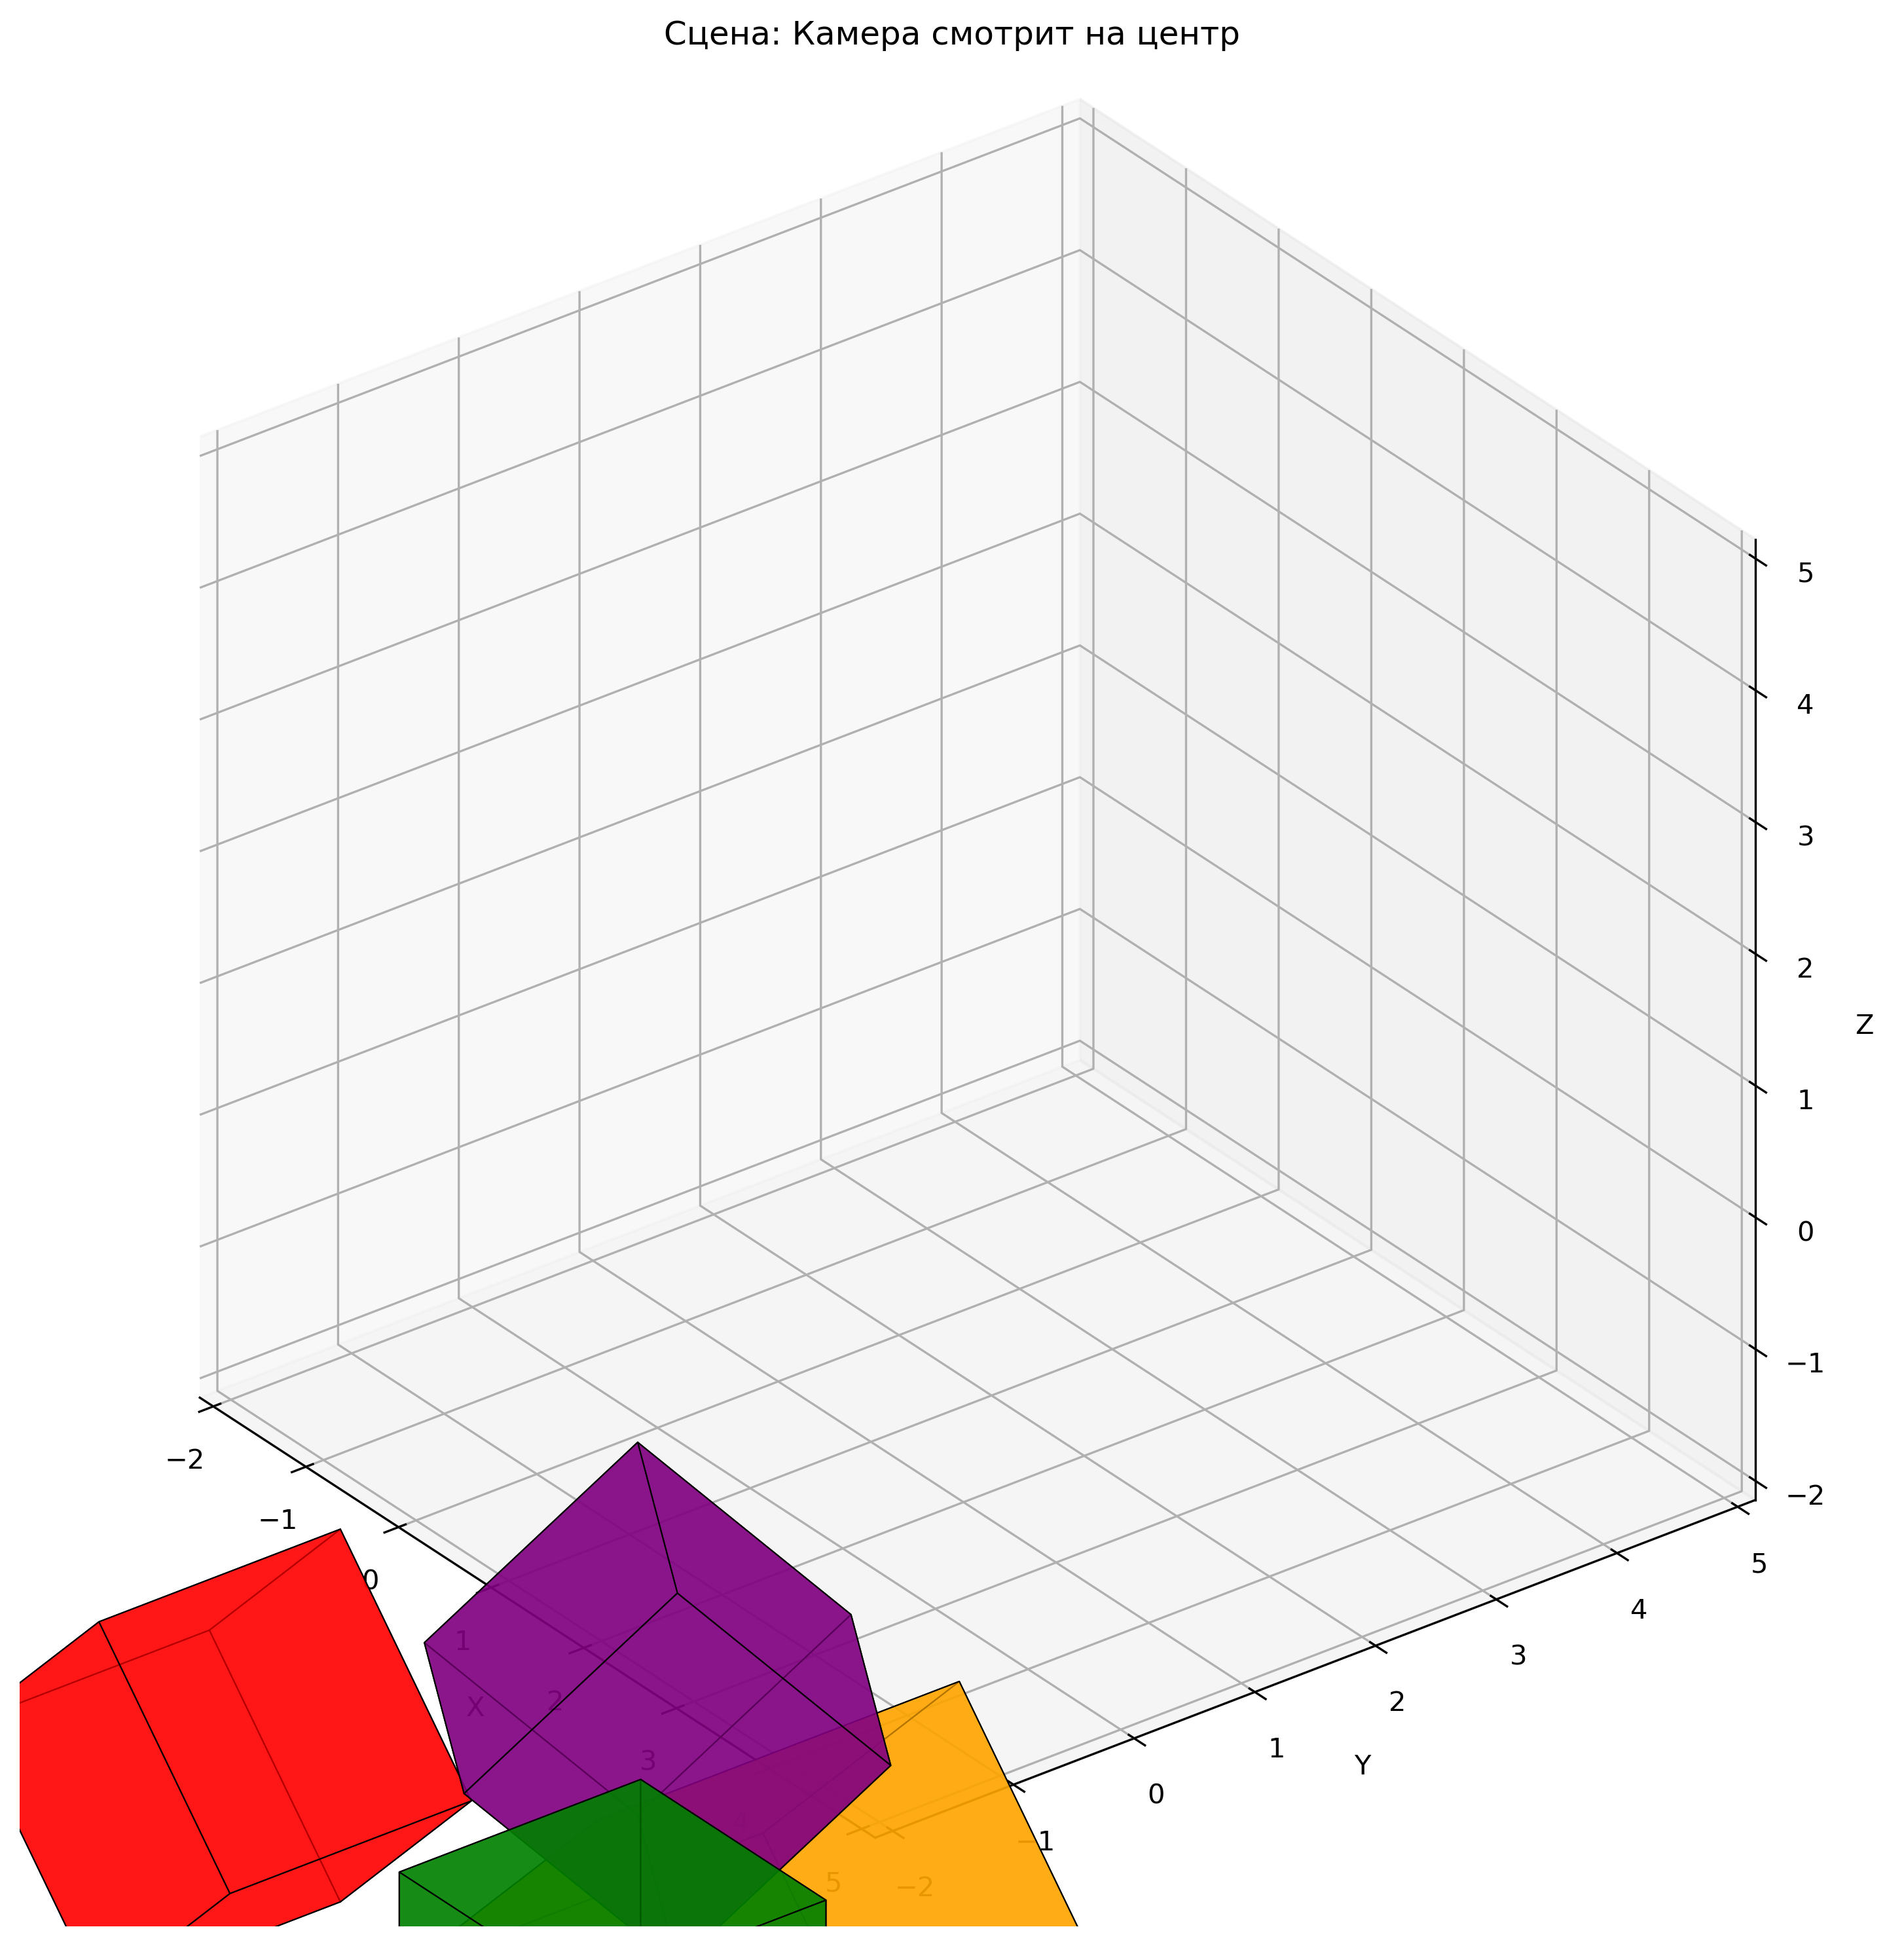
\includegraphics[width=0.8\textwidth]{images/task6/camera_look_at_center.png}
\caption{Камера смотрит на центр}
\end{figure}

\begin{figure}[H]
\centering
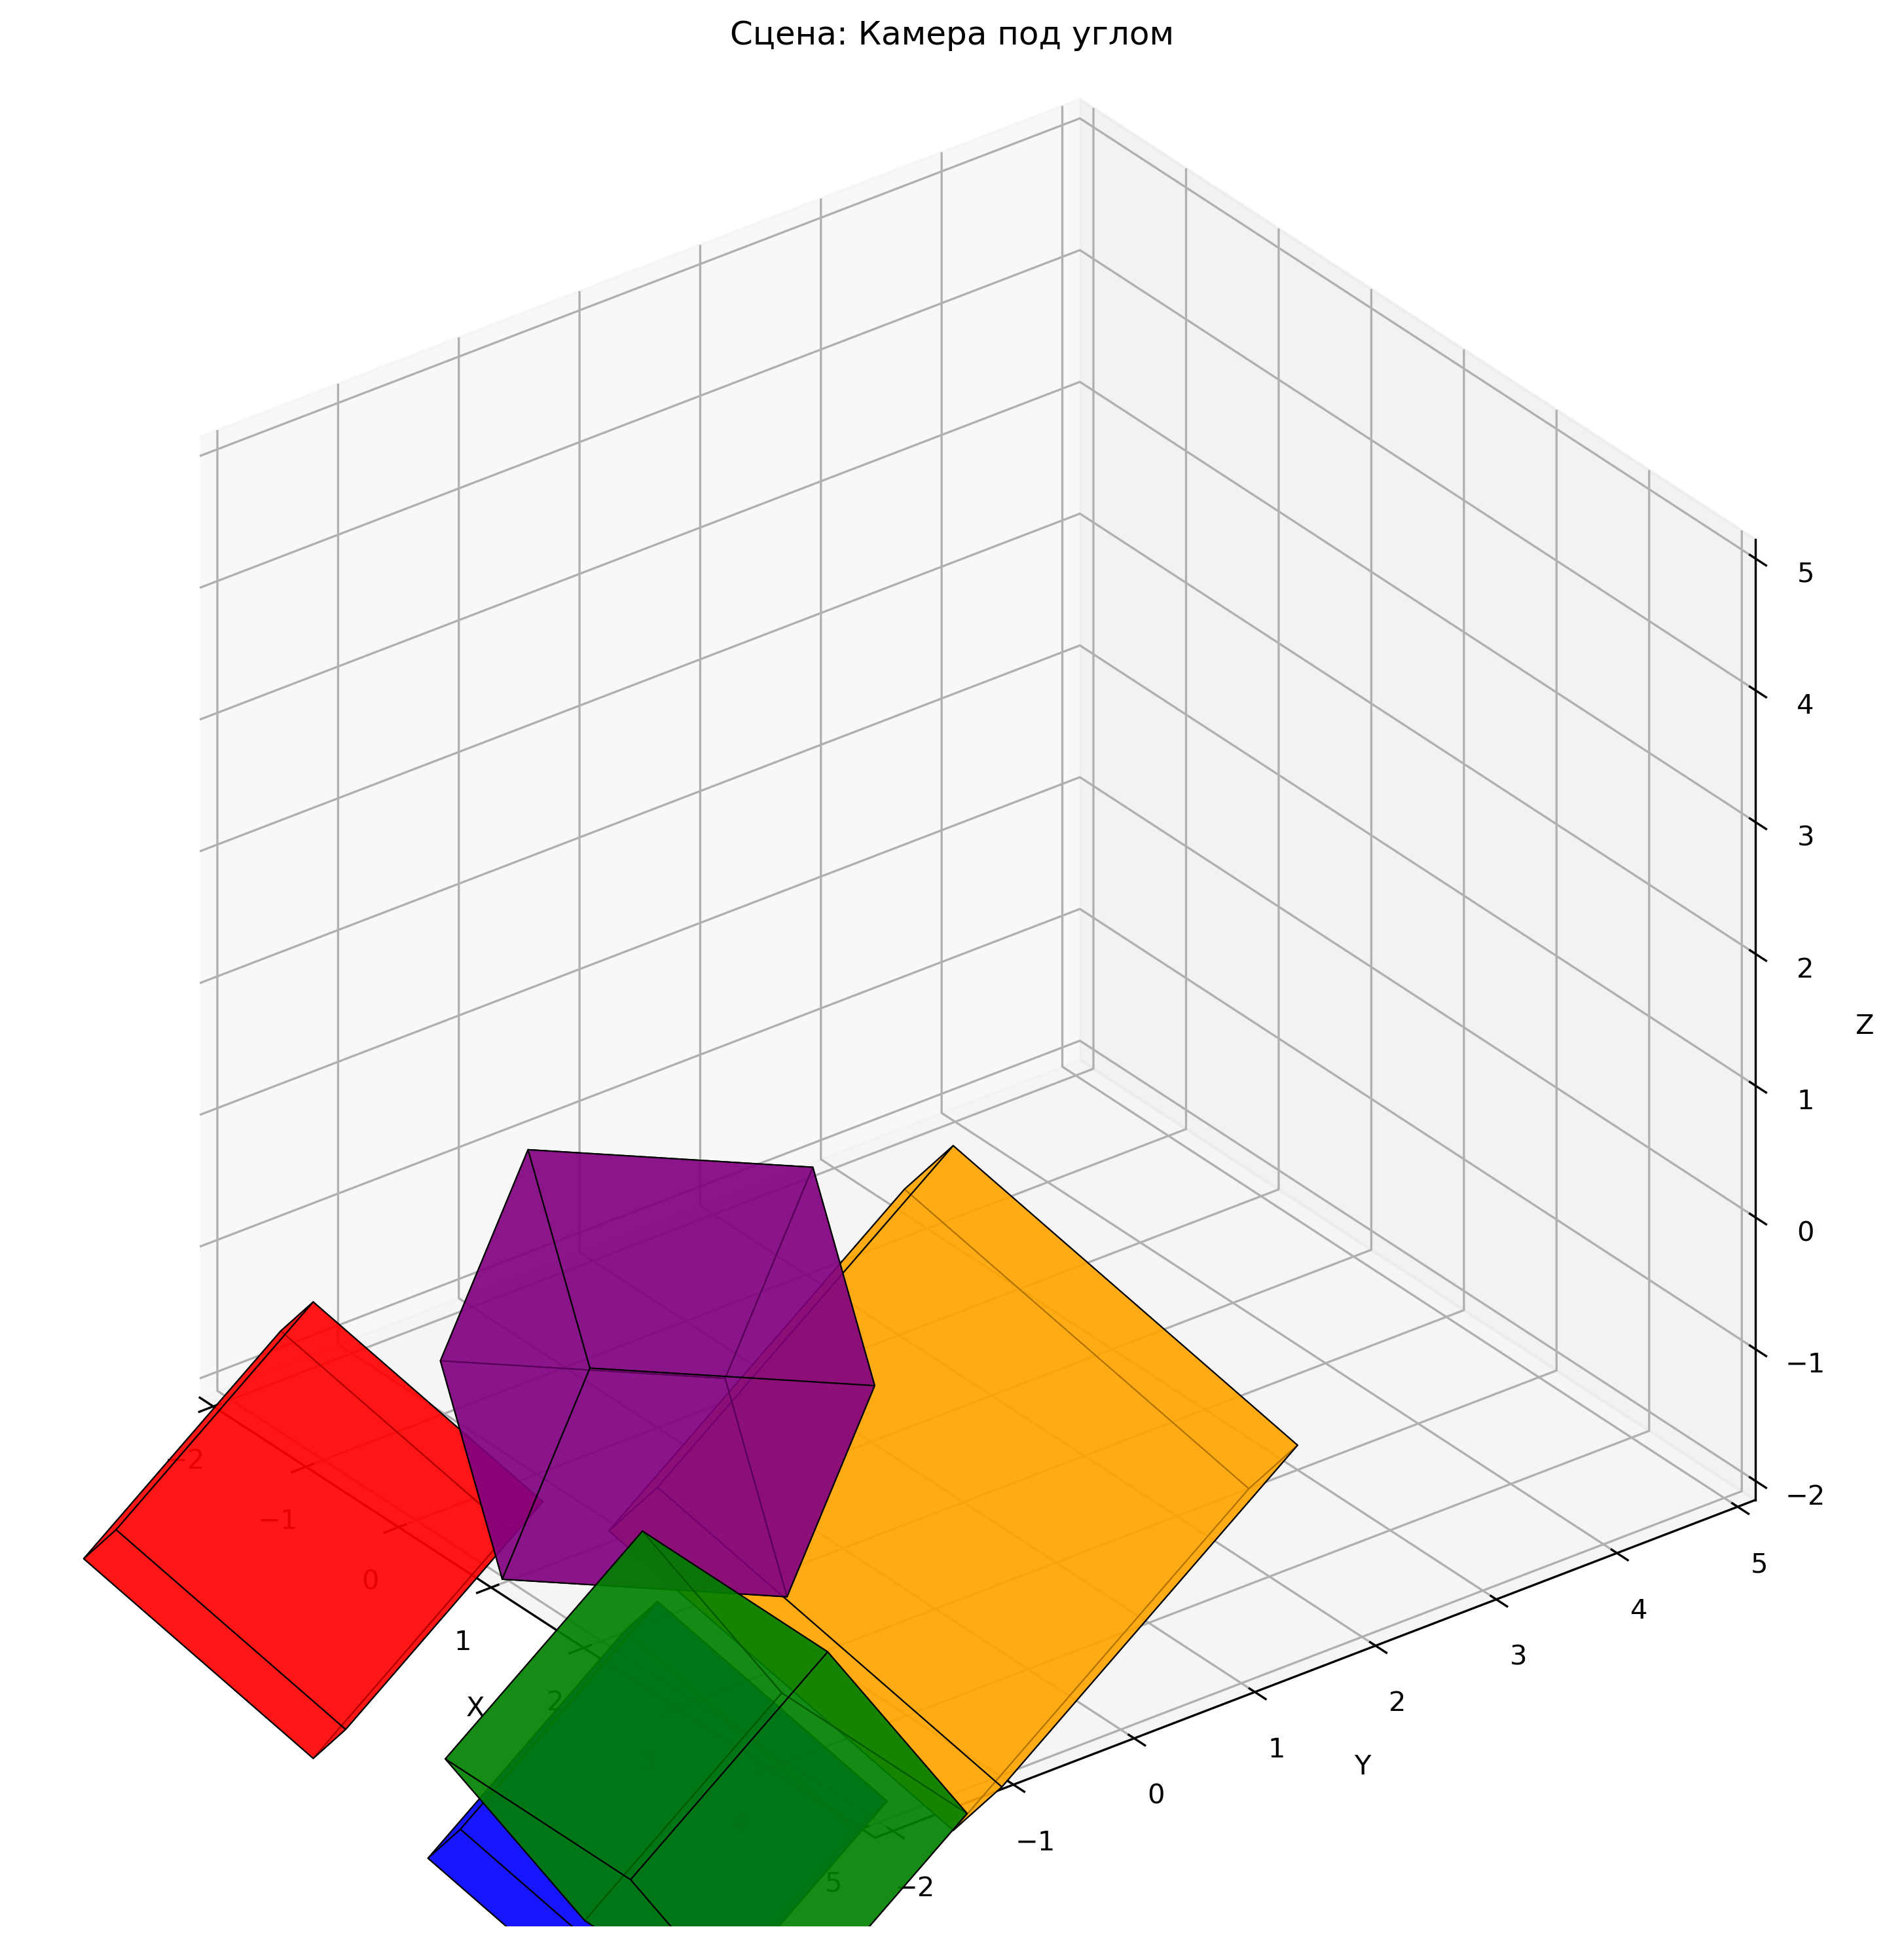
\includegraphics[width=0.8\textwidth]{images/task6/camera_angle.png}
\caption{Камера под углом}
\end{figure}

\subsection*{Обратное преобразование камеры}
\begin{itemize}
    \item $C^{-1}$ восстанавливает исходную сцену
    \item Ошибка восстановления минимальна
    \item Преобразование камеры обратимо
\end{itemize}

\section*{Задание 7: Перспективные преобразования}

\subsection*{Постановка задачи}
Реализовать перспективные преобразования и исследовать их влияние на геометрию объектов.

\subsection*{Математические основы}
Матрица перспективного преобразования:
\begin{equation}
P = \begin{pmatrix}
1 & 0 & 0 & 0 \\
0 & 1 & 0 & 0 \\
0 & 0 & 1 & 0 \\
0 & 0 & \frac{1}{d} & 0
\end{pmatrix}
\end{equation}

где $d$ - расстояние до плоскости проекции.

\subsection*{Результаты}
Исследованы различные перспективные преобразования:

\begin{figure}[H]
\centering
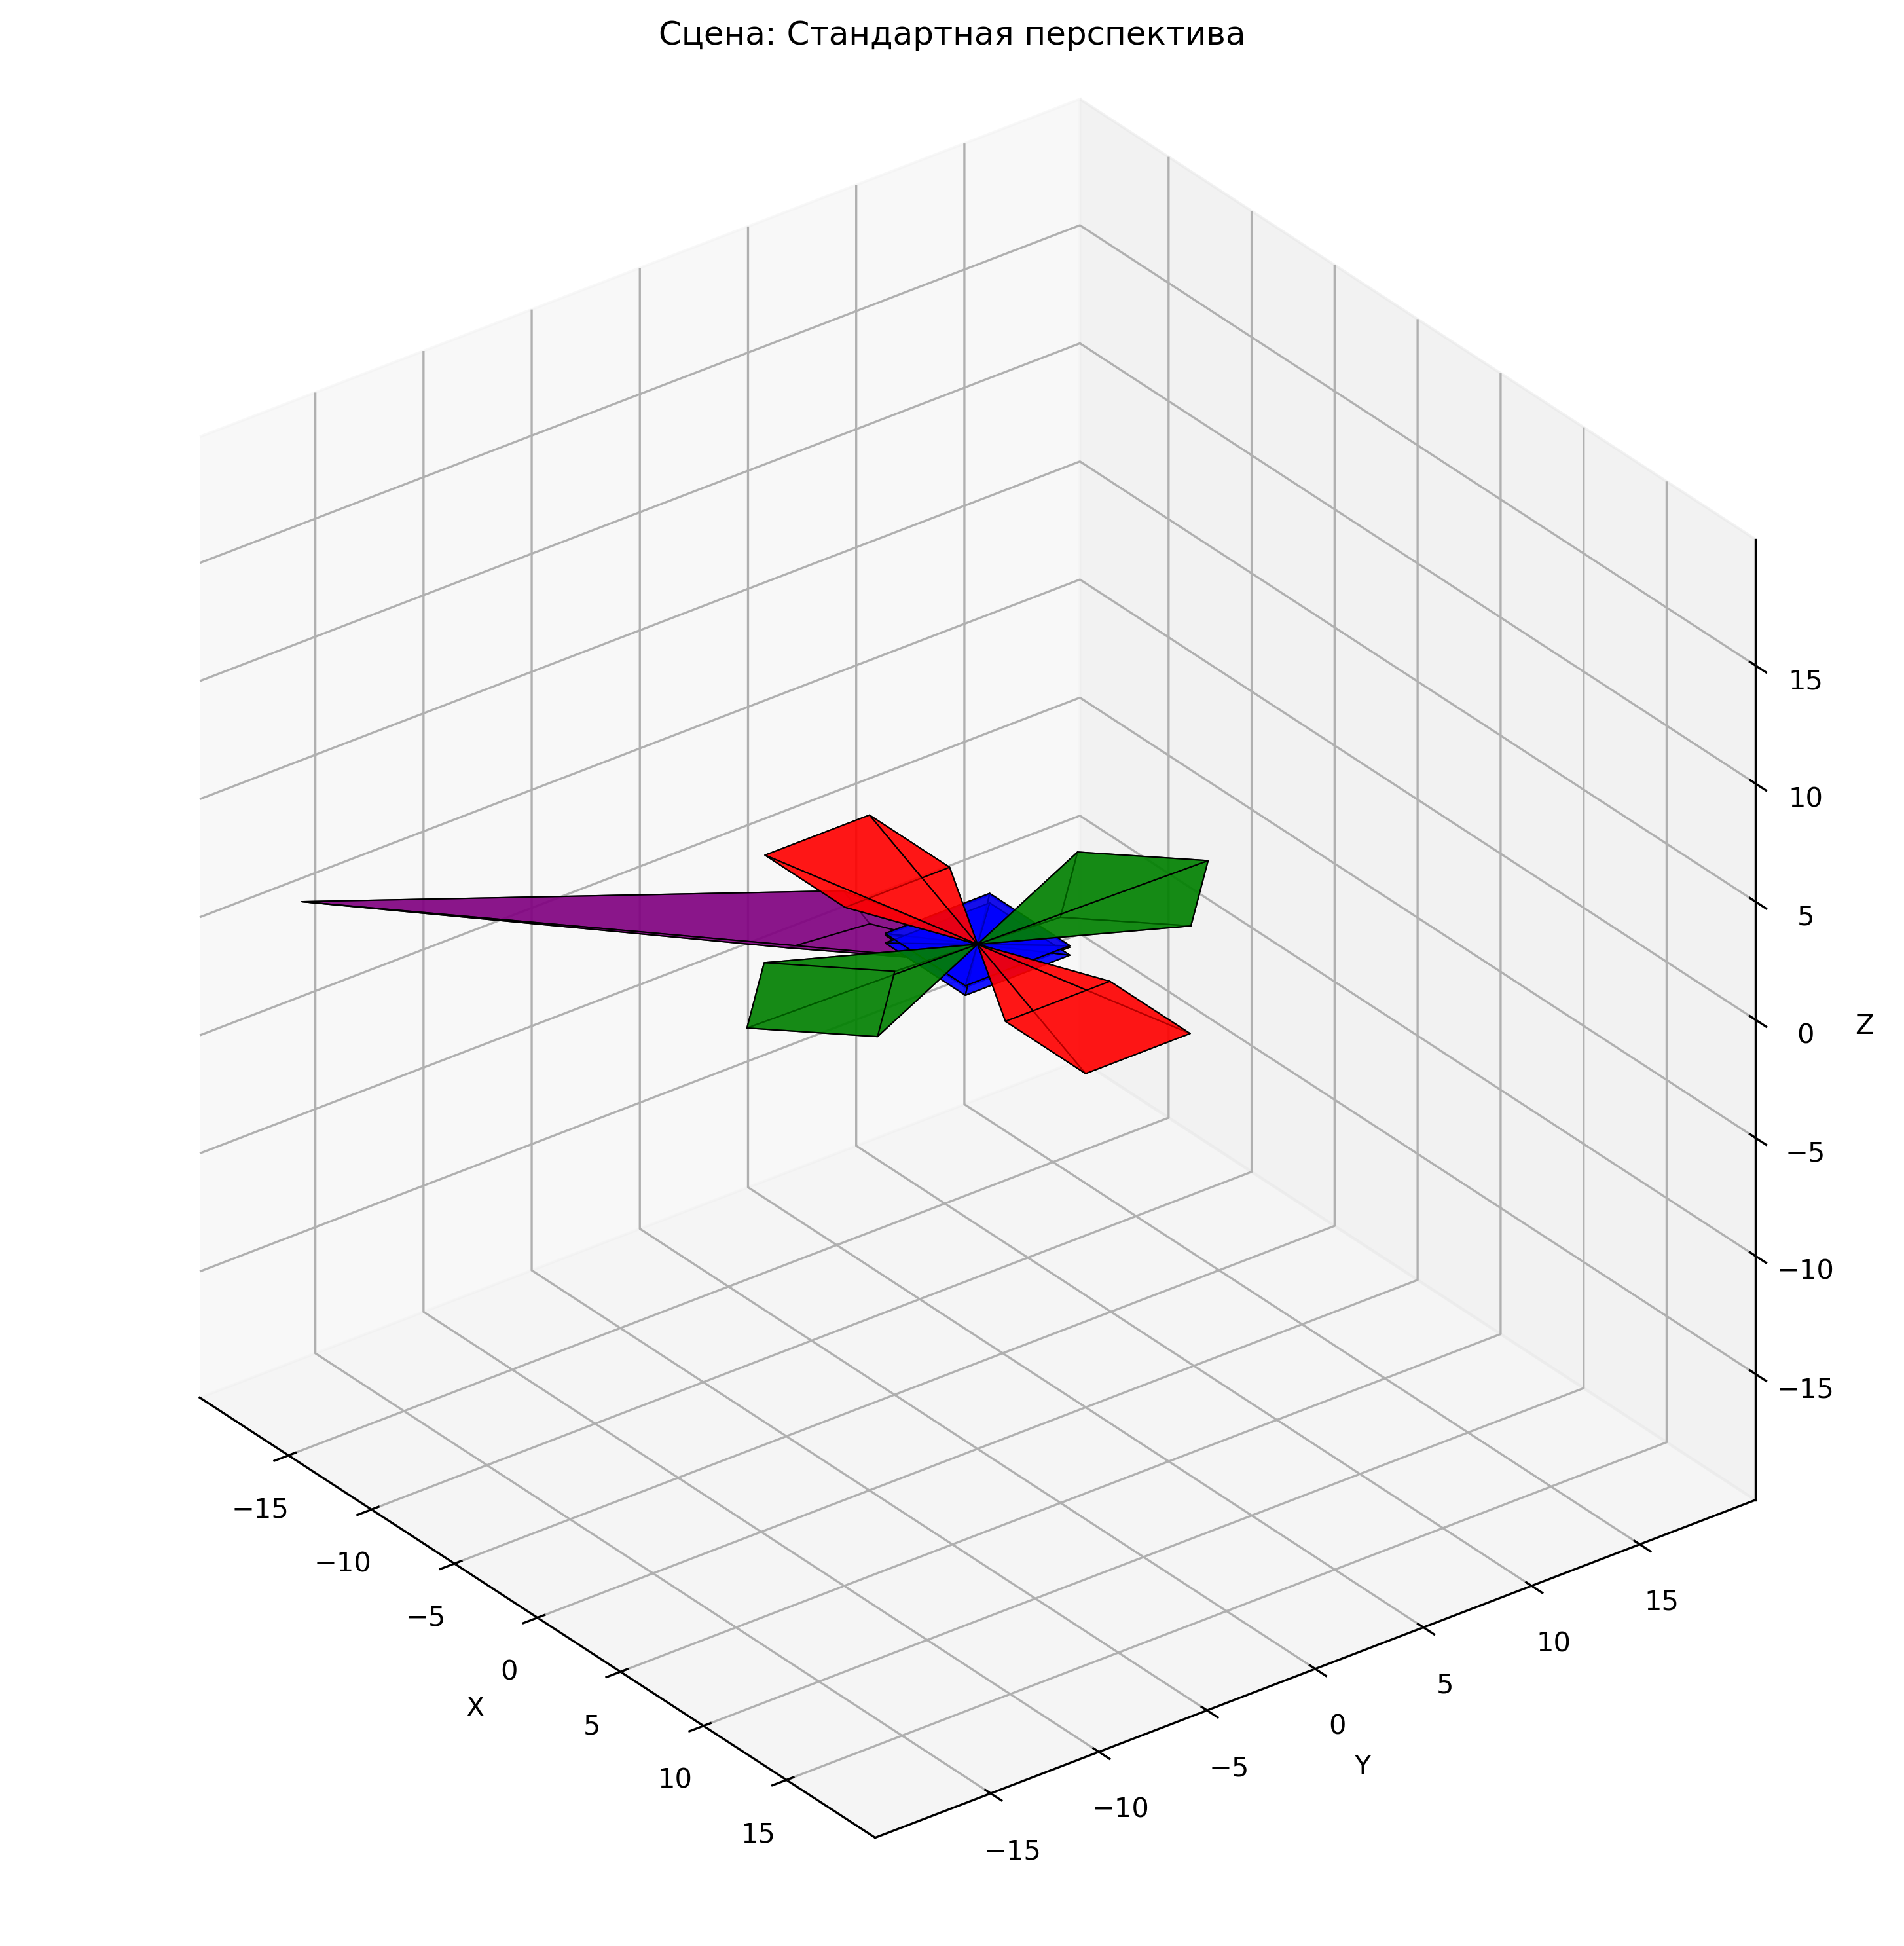
\includegraphics[width=0.8\textwidth]{images/task7/perspective_standard.png}
\caption{Стандартная перспектива}
\end{figure}

\begin{figure}[H]
\centering
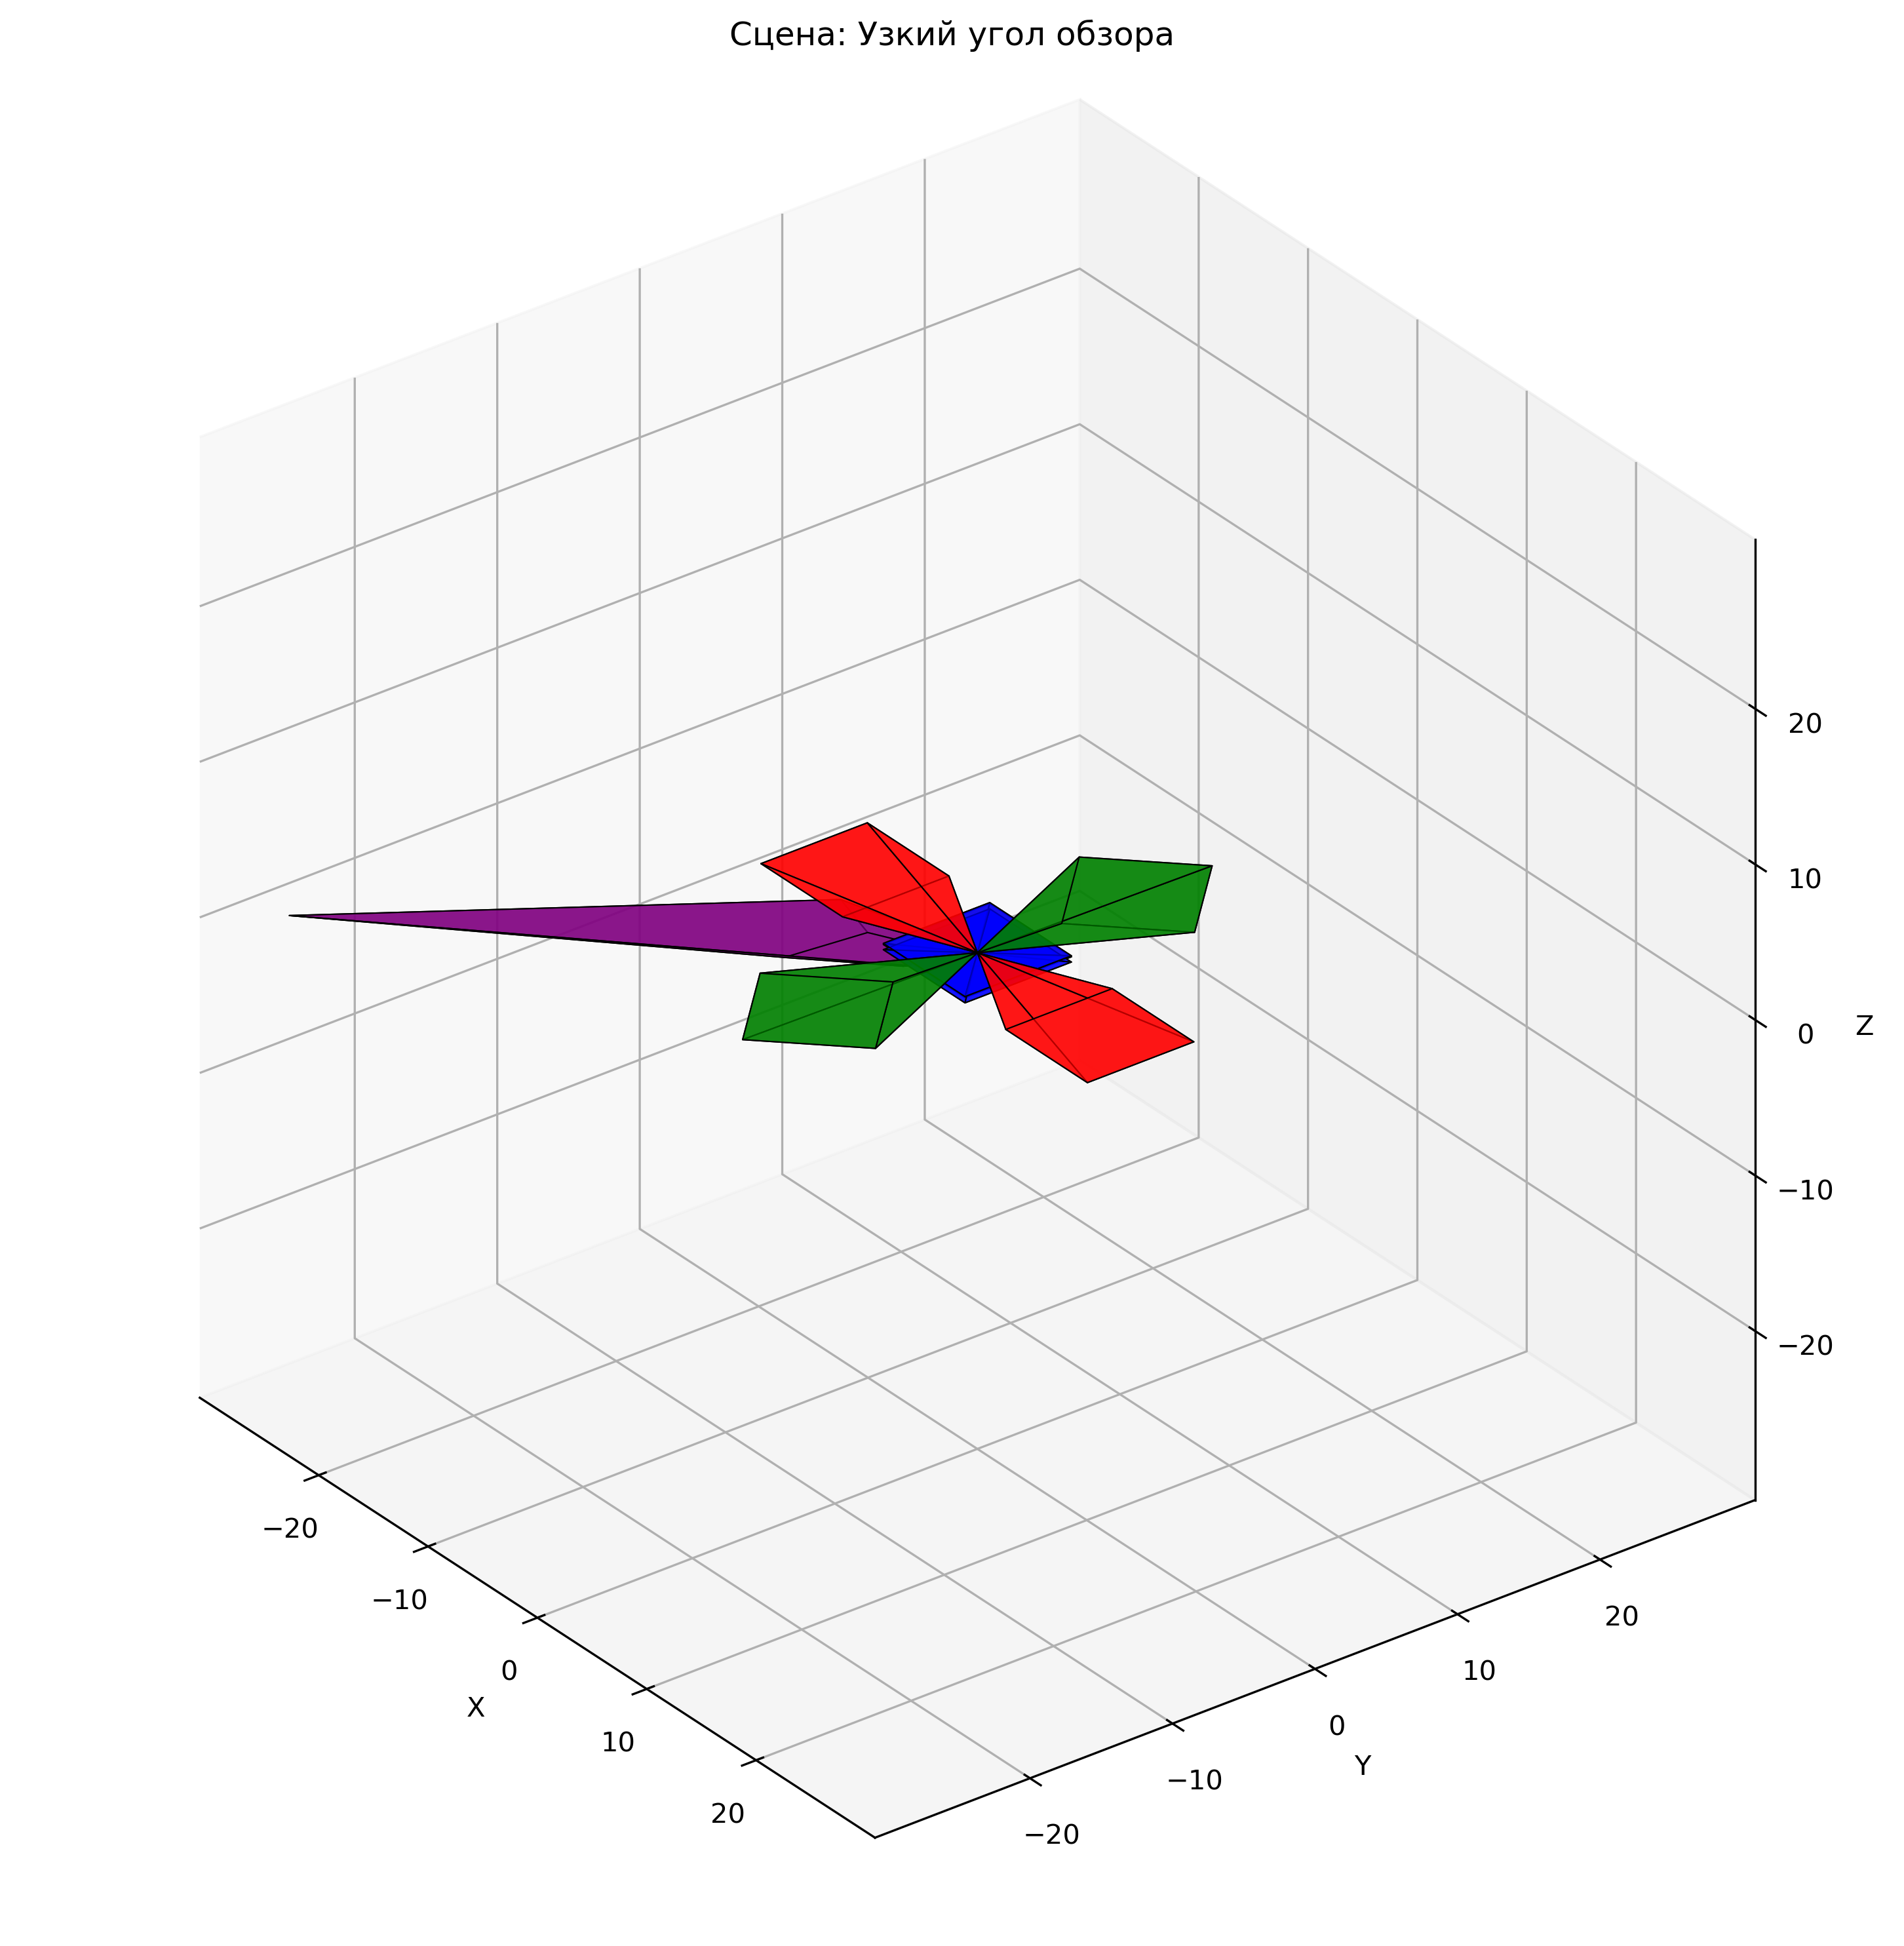
\includegraphics[width=0.8\textwidth]{images/task7/perspective_narrow.png}
\caption{Узкая перспектива}
\end{figure}

\begin{figure}[H]
\centering
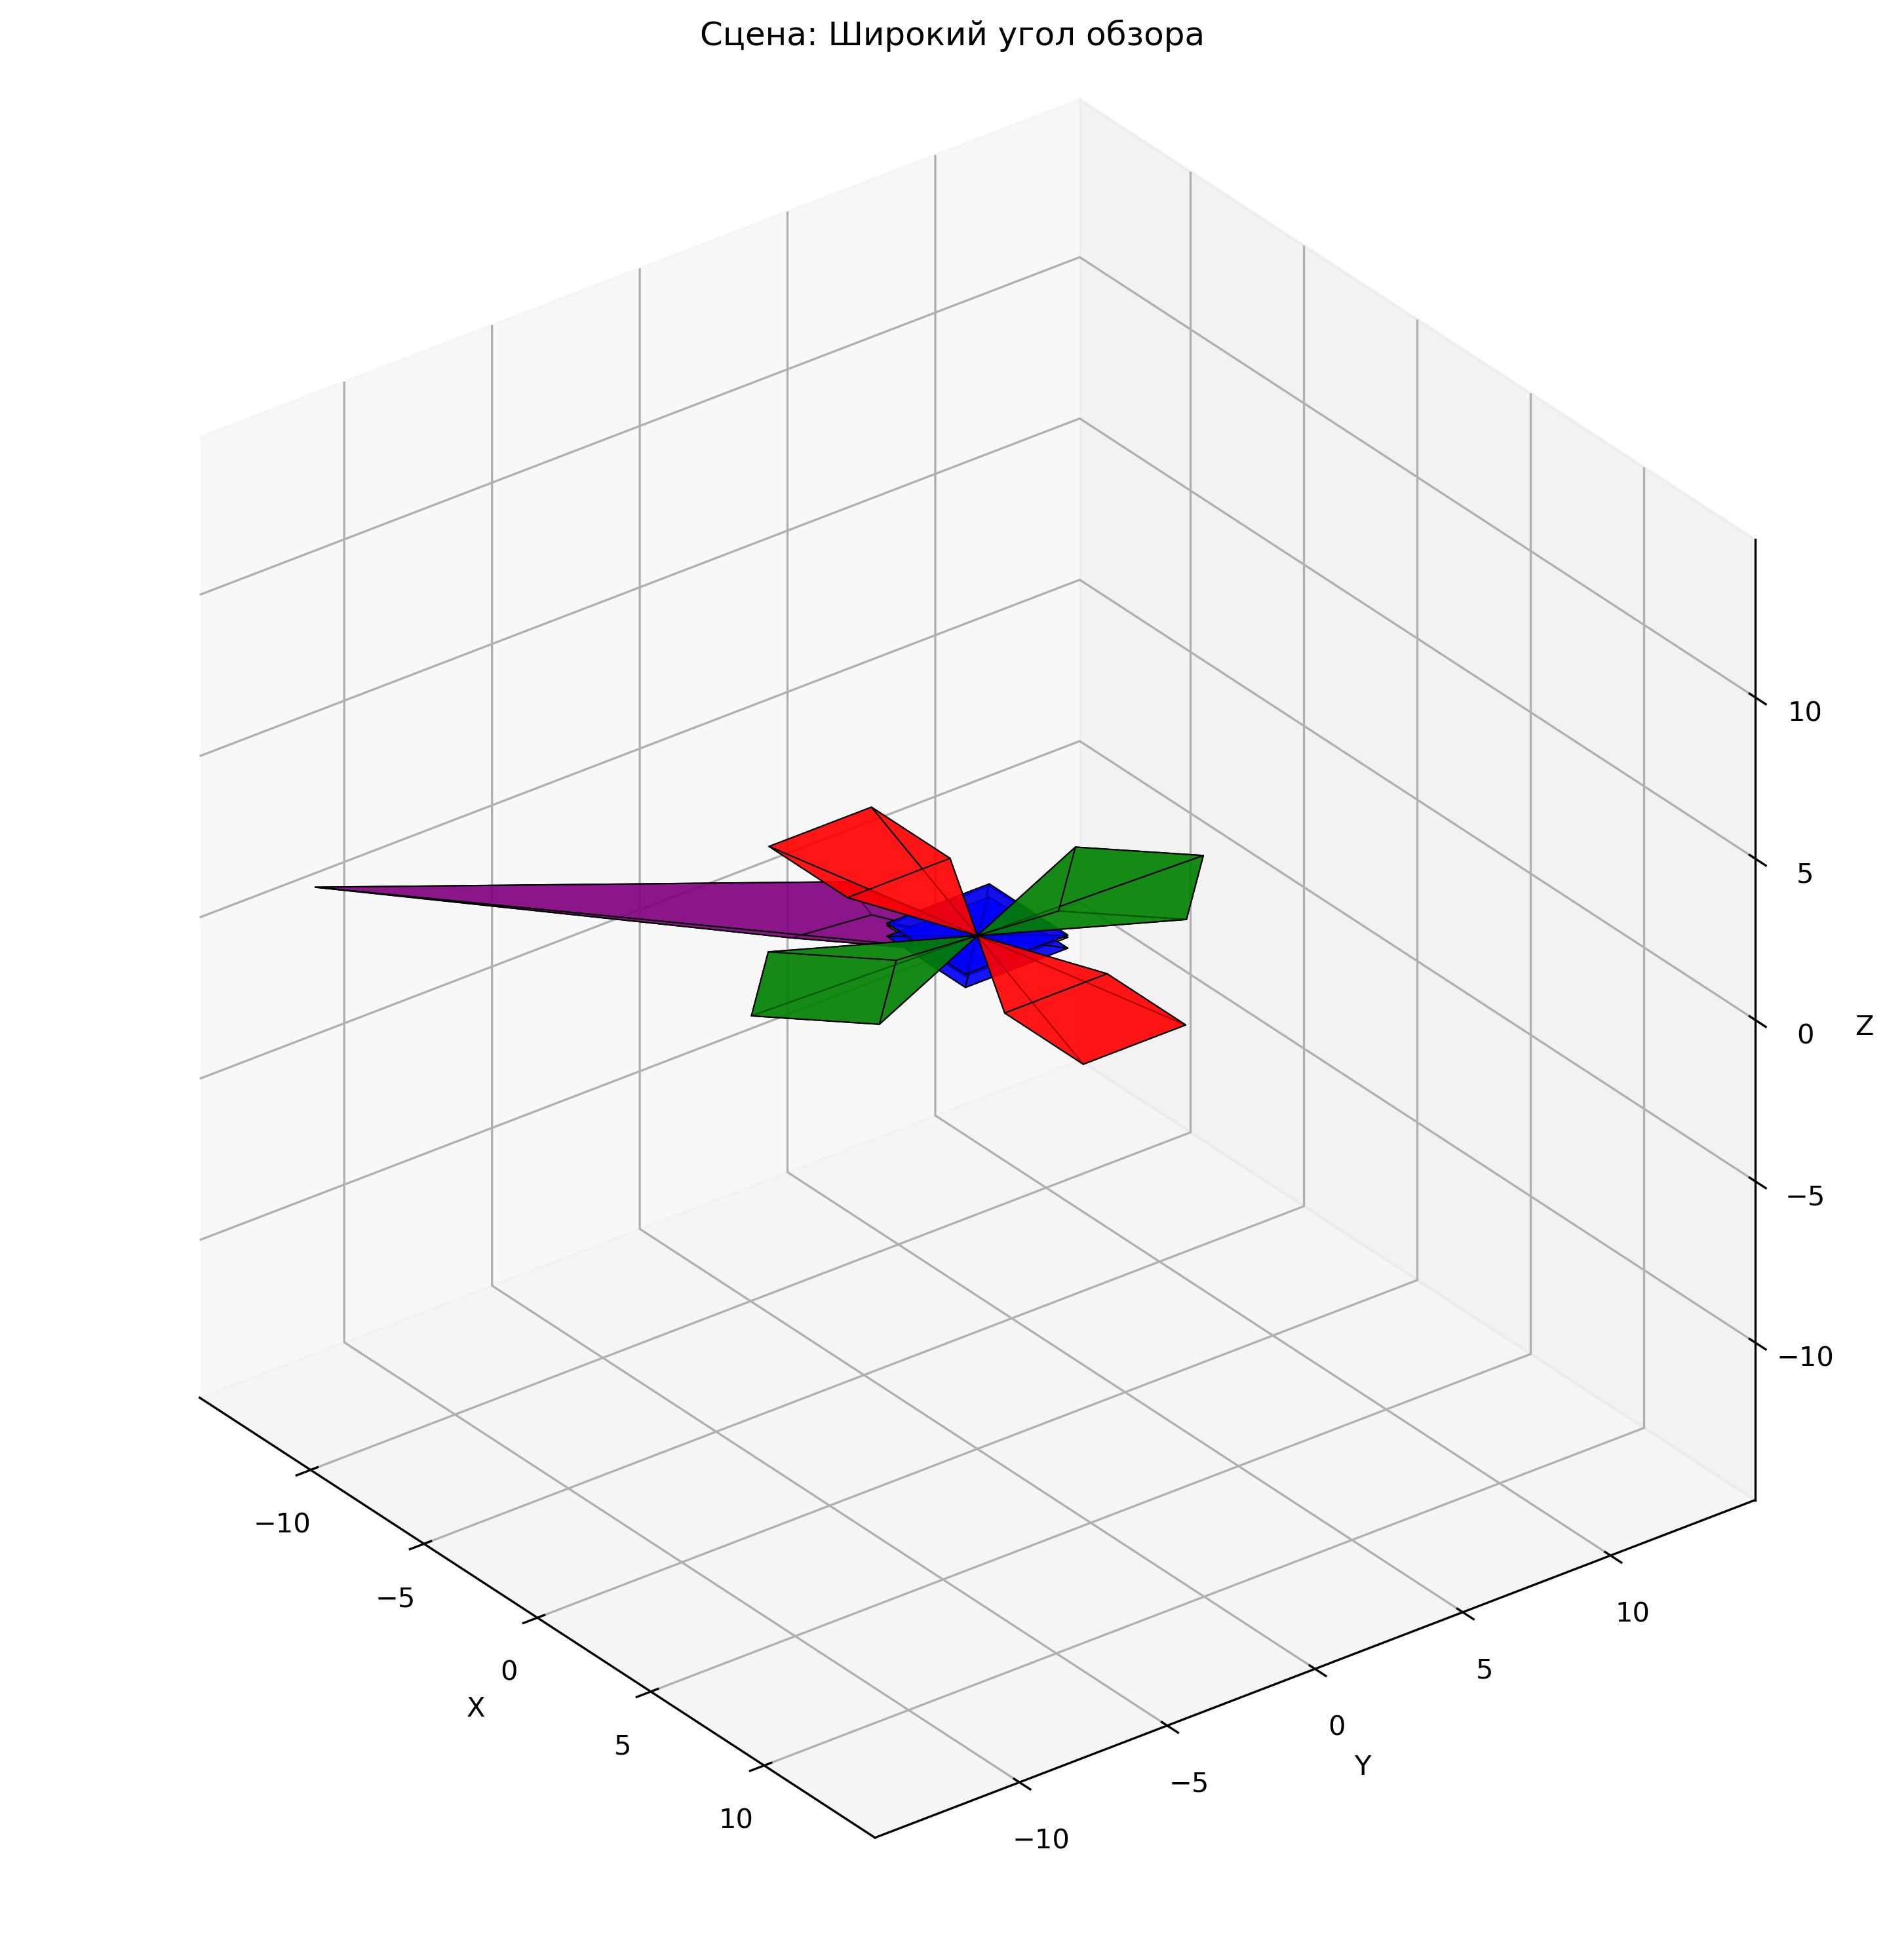
\includegraphics[width=0.8\textwidth]{images/task7/perspective_wide.png}
\caption{Широкая перспектива}
\end{figure}

\begin{figure}[H]
\centering
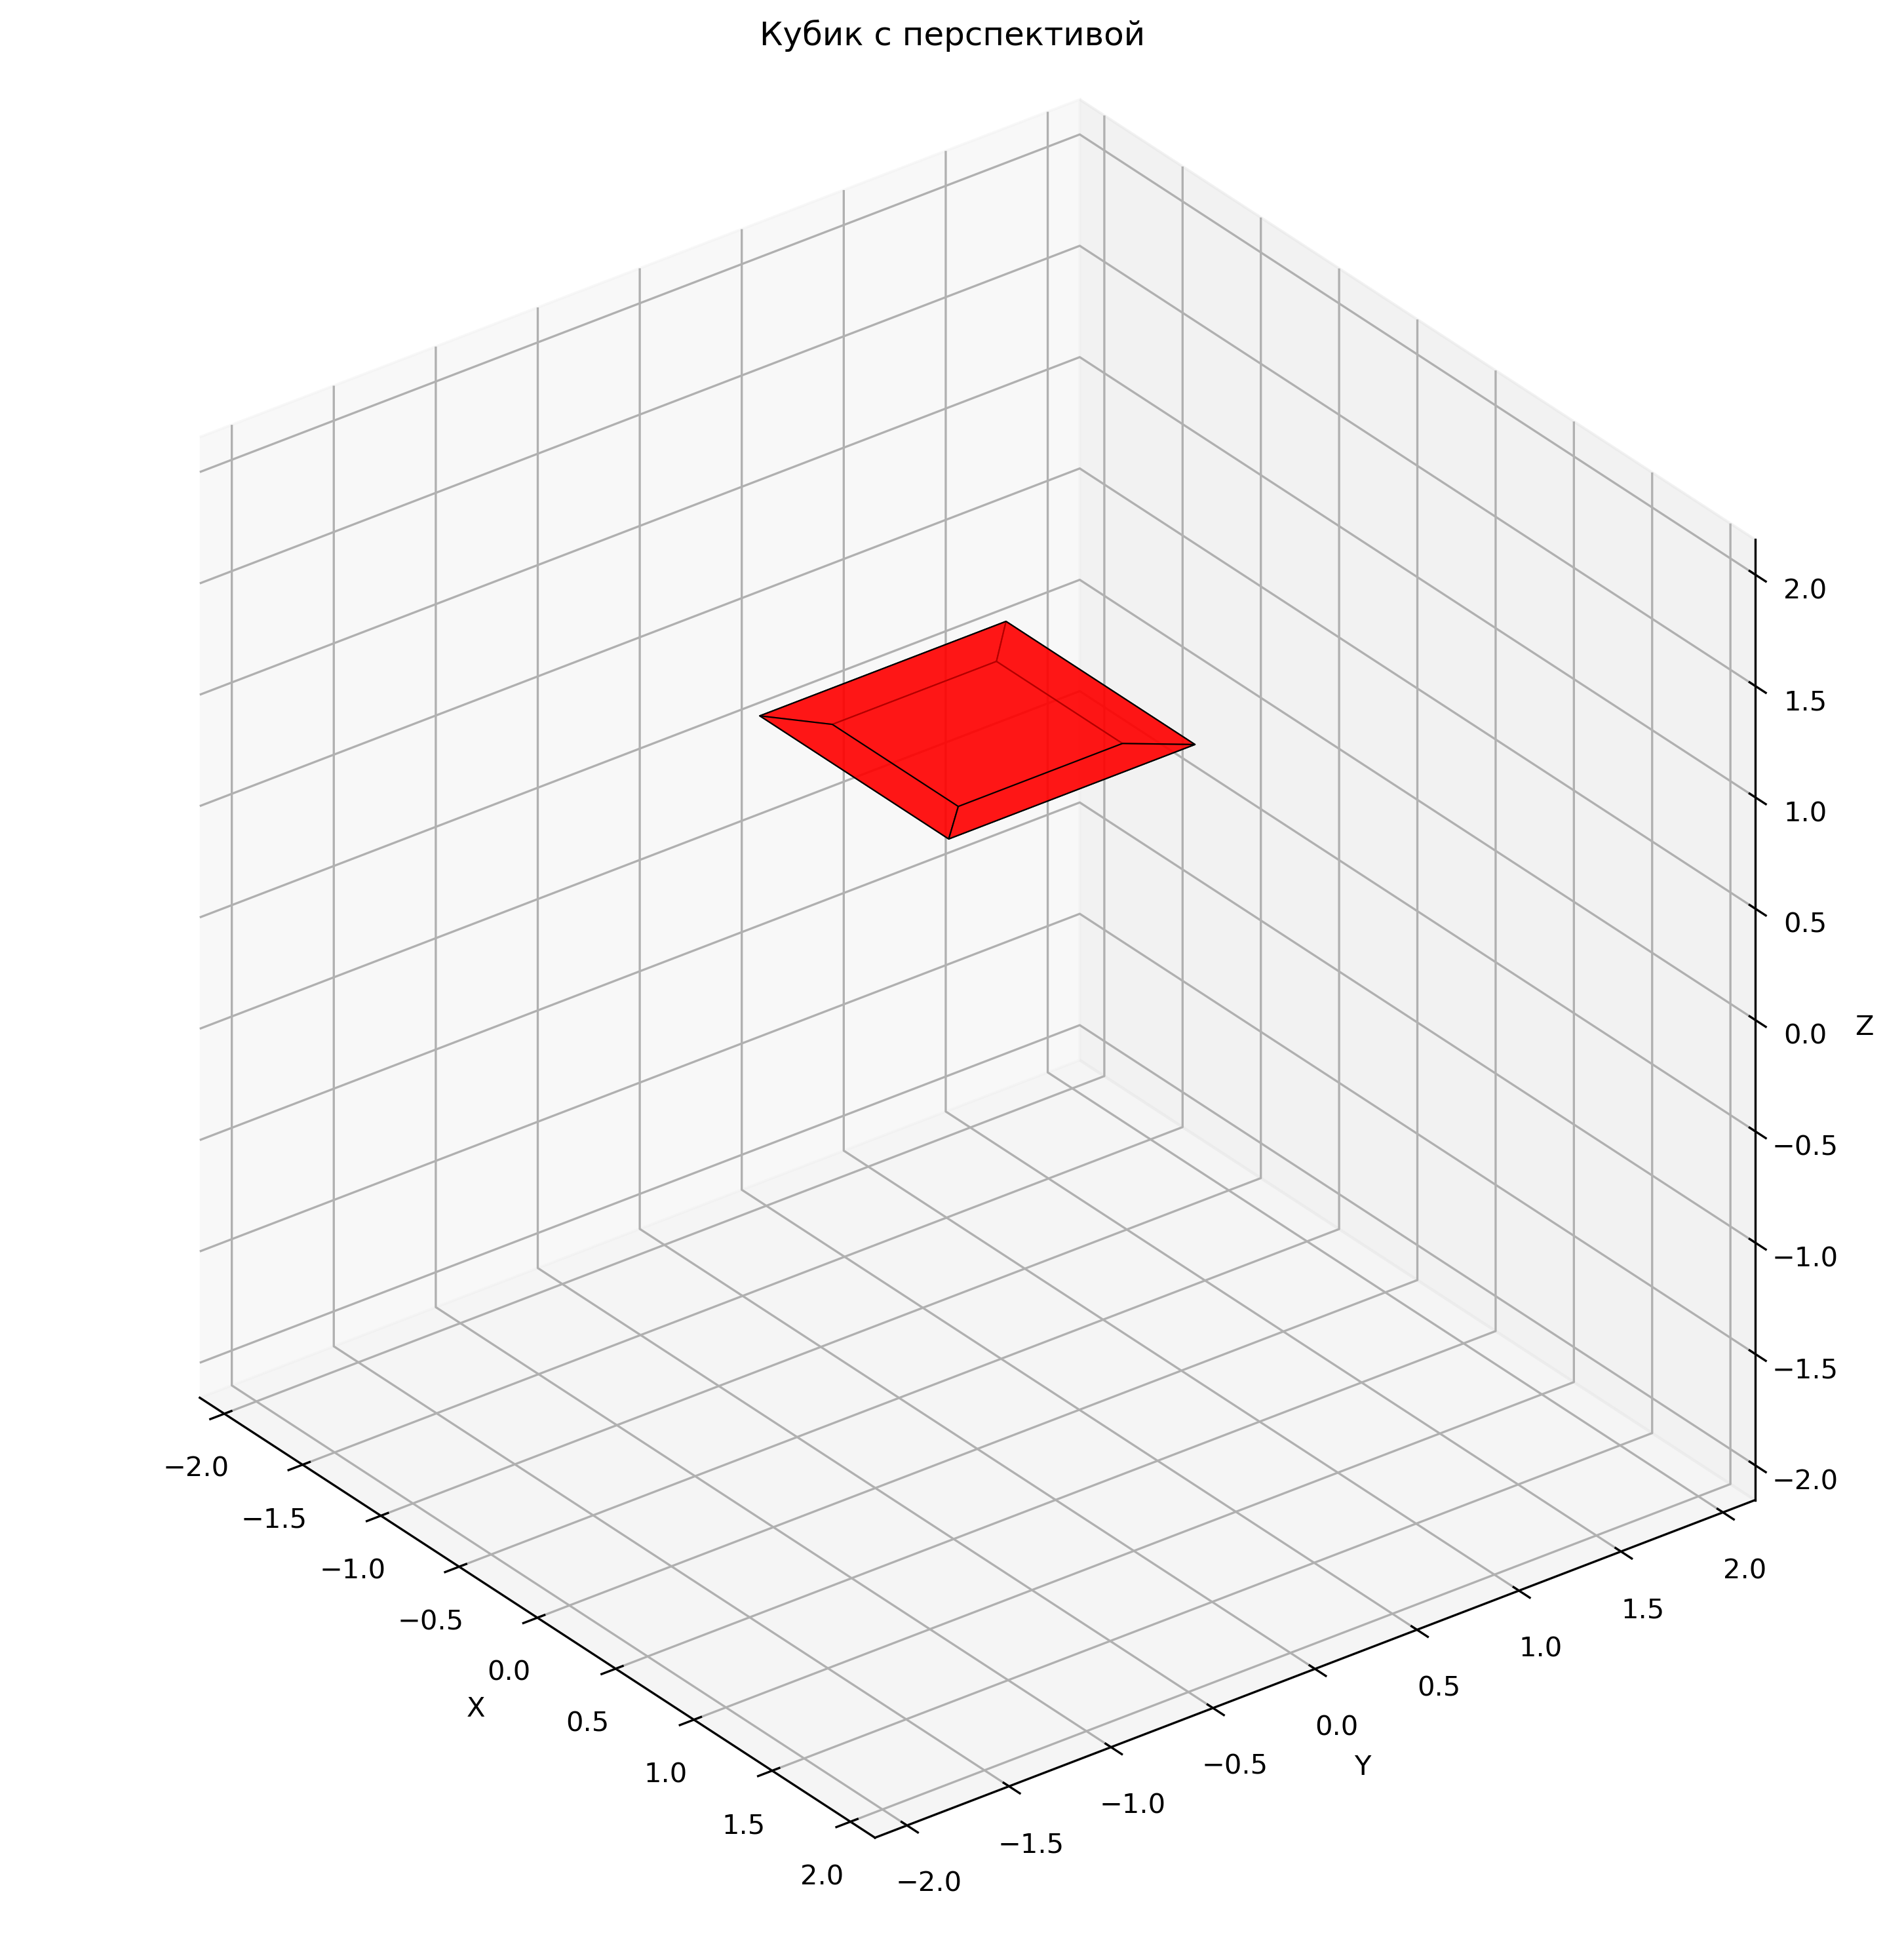
\includegraphics[width=0.8\textwidth]{images/task7/perspective_cube.png}
\caption{Перспектива кубика}
\end{figure}

\subsection*{Анализ эффектов}
\begin{itemize}
    \item Уменьшение $d$ усиливает эффект перспективы
    \item Параллельные линии сходятся в точку схода
    \item Объекты, расположенные дальше, кажутся меньше
    \item Перспектива создает иллюзию глубины
\end{itemize}

\section*{Задание 8: Построение домика (почти Blender)}

\subsection*{Постановка задачи}
Создать сложную 3D сцену - домик, используя все изученные преобразования, и продемонстрировать процесс построения.

\subsection*{Структура домика}
Домик состоит из 12 элементов:
\begin{itemize}
    \item Фундамент (8×6×1)
    \item 4 стены (6×0.4×4 и 0.4×6×4)
    \item 2 части крыши (5.46×6×0.55)
    \item Дверь (1.6×0.2×3)
    \item 2 окна (1.6×0.2×1.6)
    \item Дымоход (0.6×0.6×2)
    \item Труба (0.4×0.4×1)
\end{itemize}

\subsection*{Процесс построения}

\begin{figure}[H]
\centering
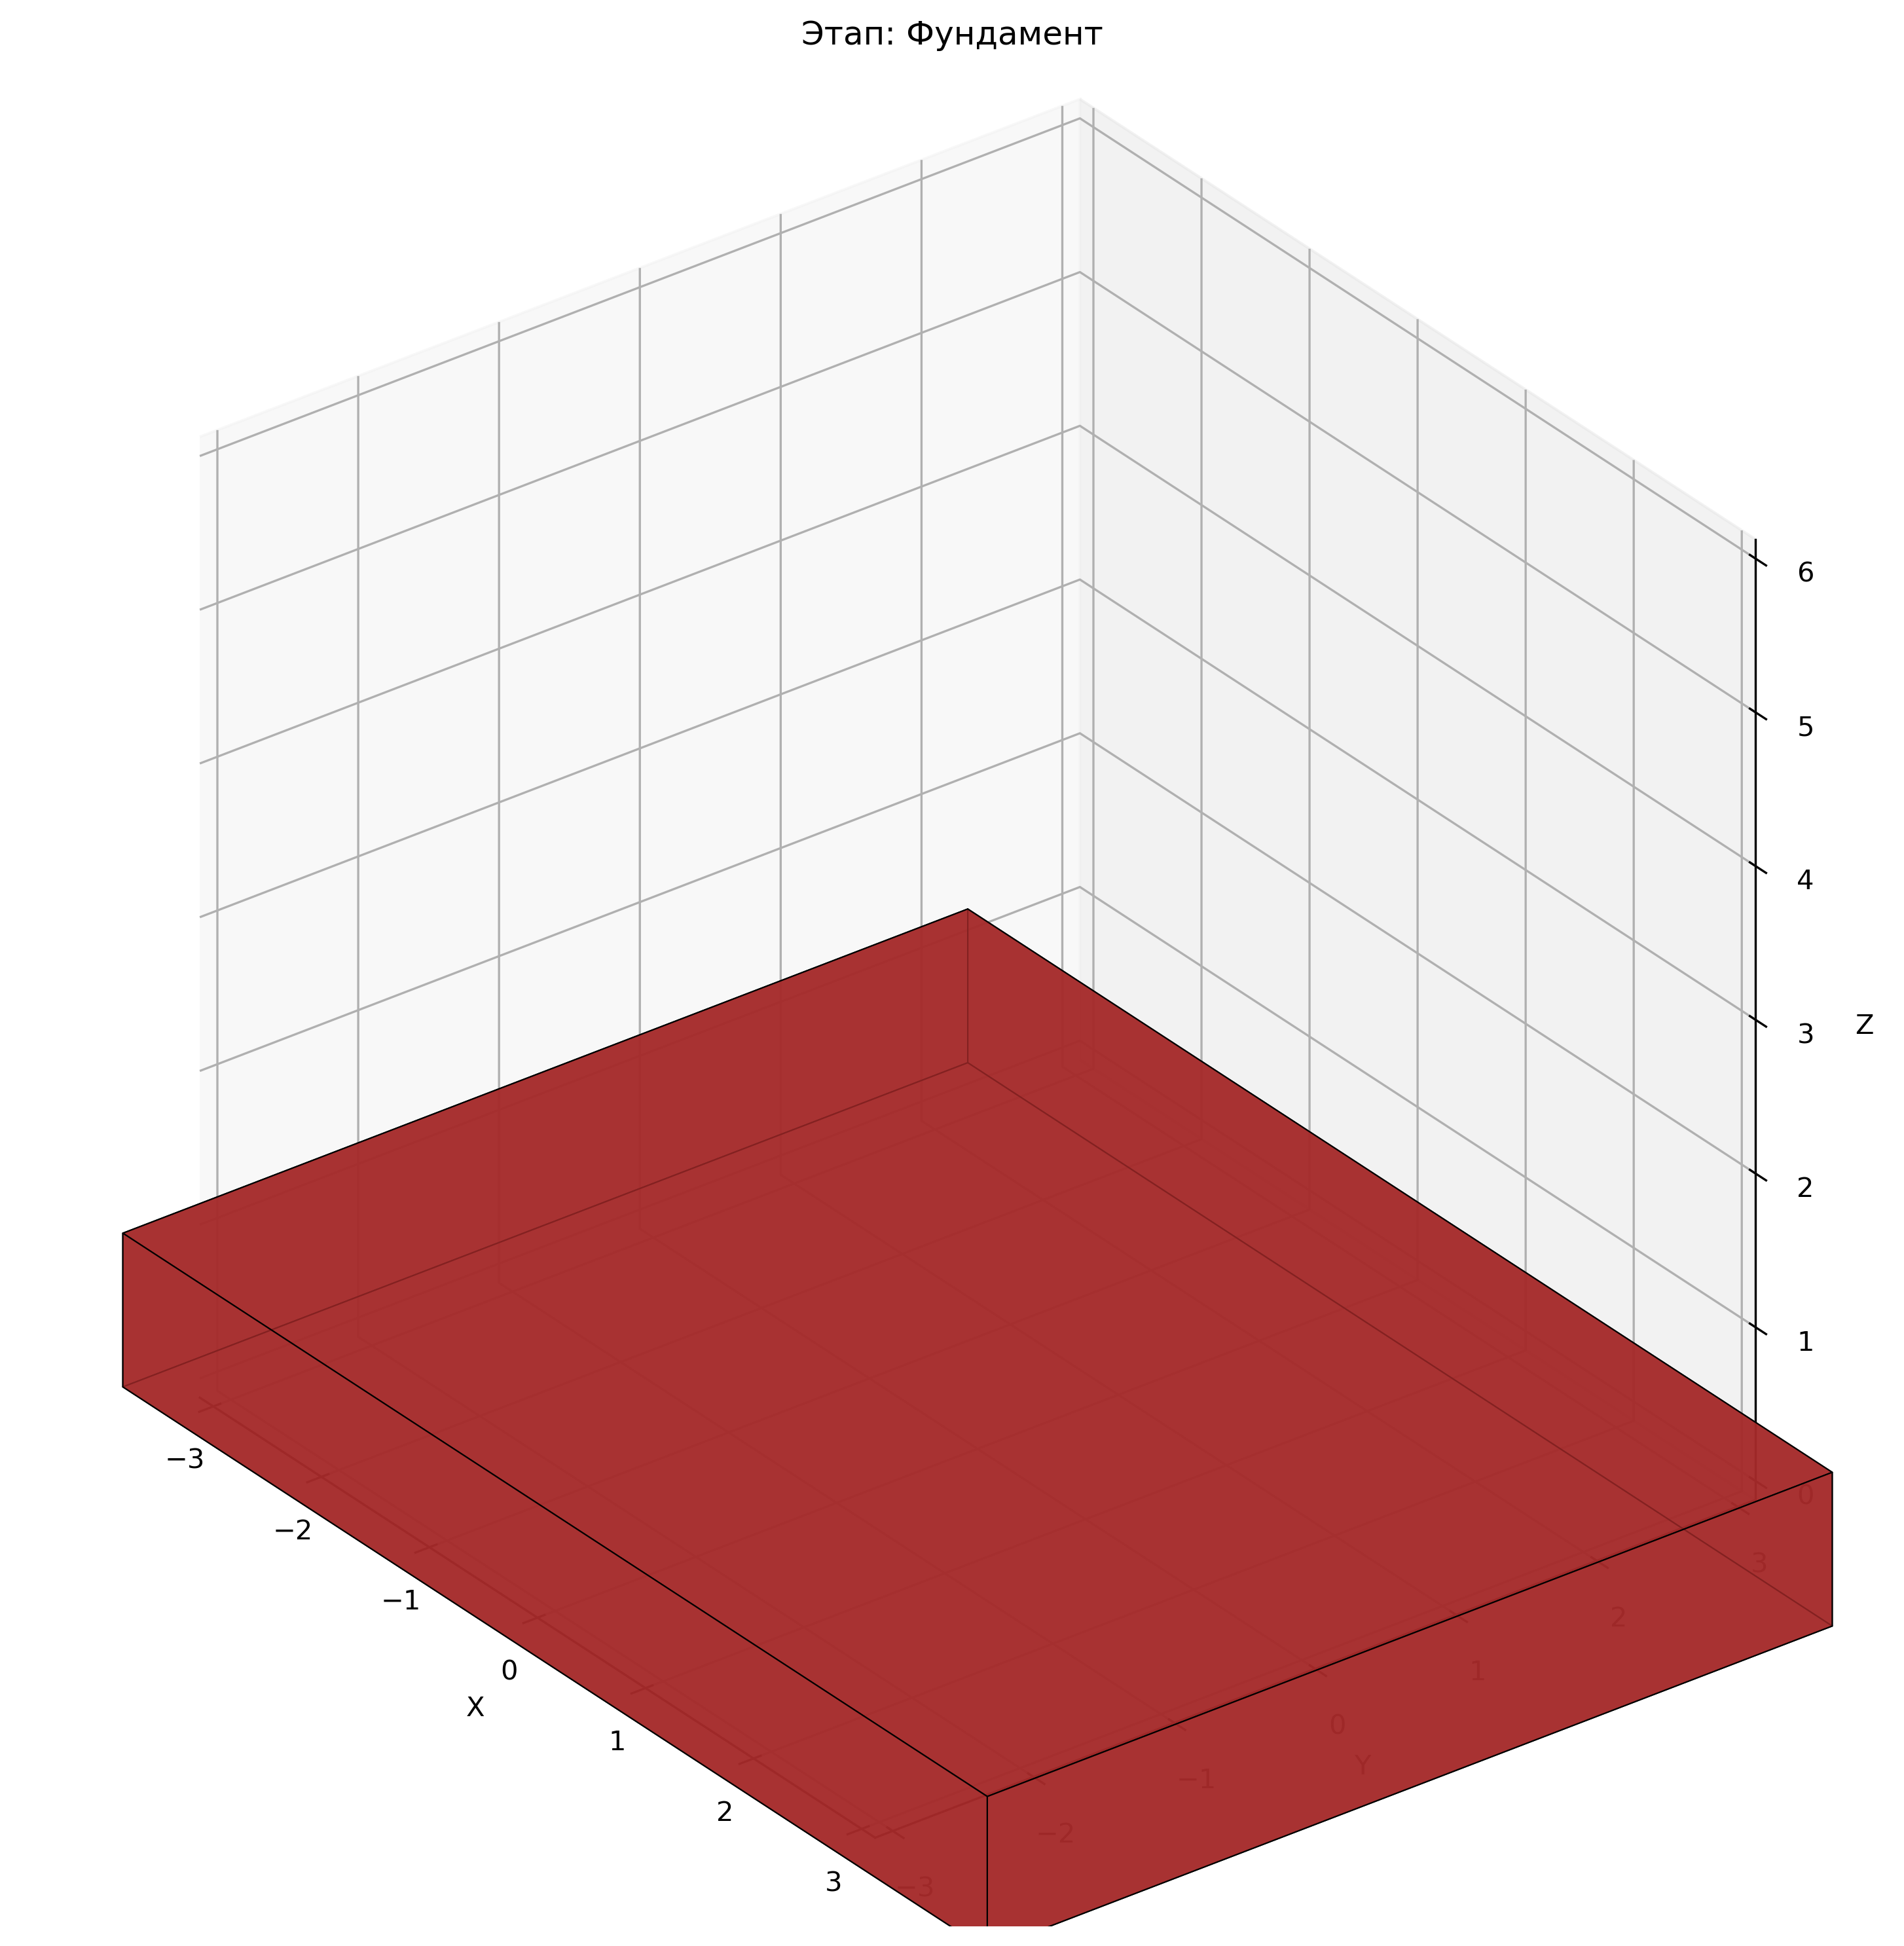
\includegraphics[width=0.8\textwidth]{images/task8/construction_фундамент.png}
\caption{Этап 1: Фундамент}
\end{figure}

\begin{figure}[H]
\centering
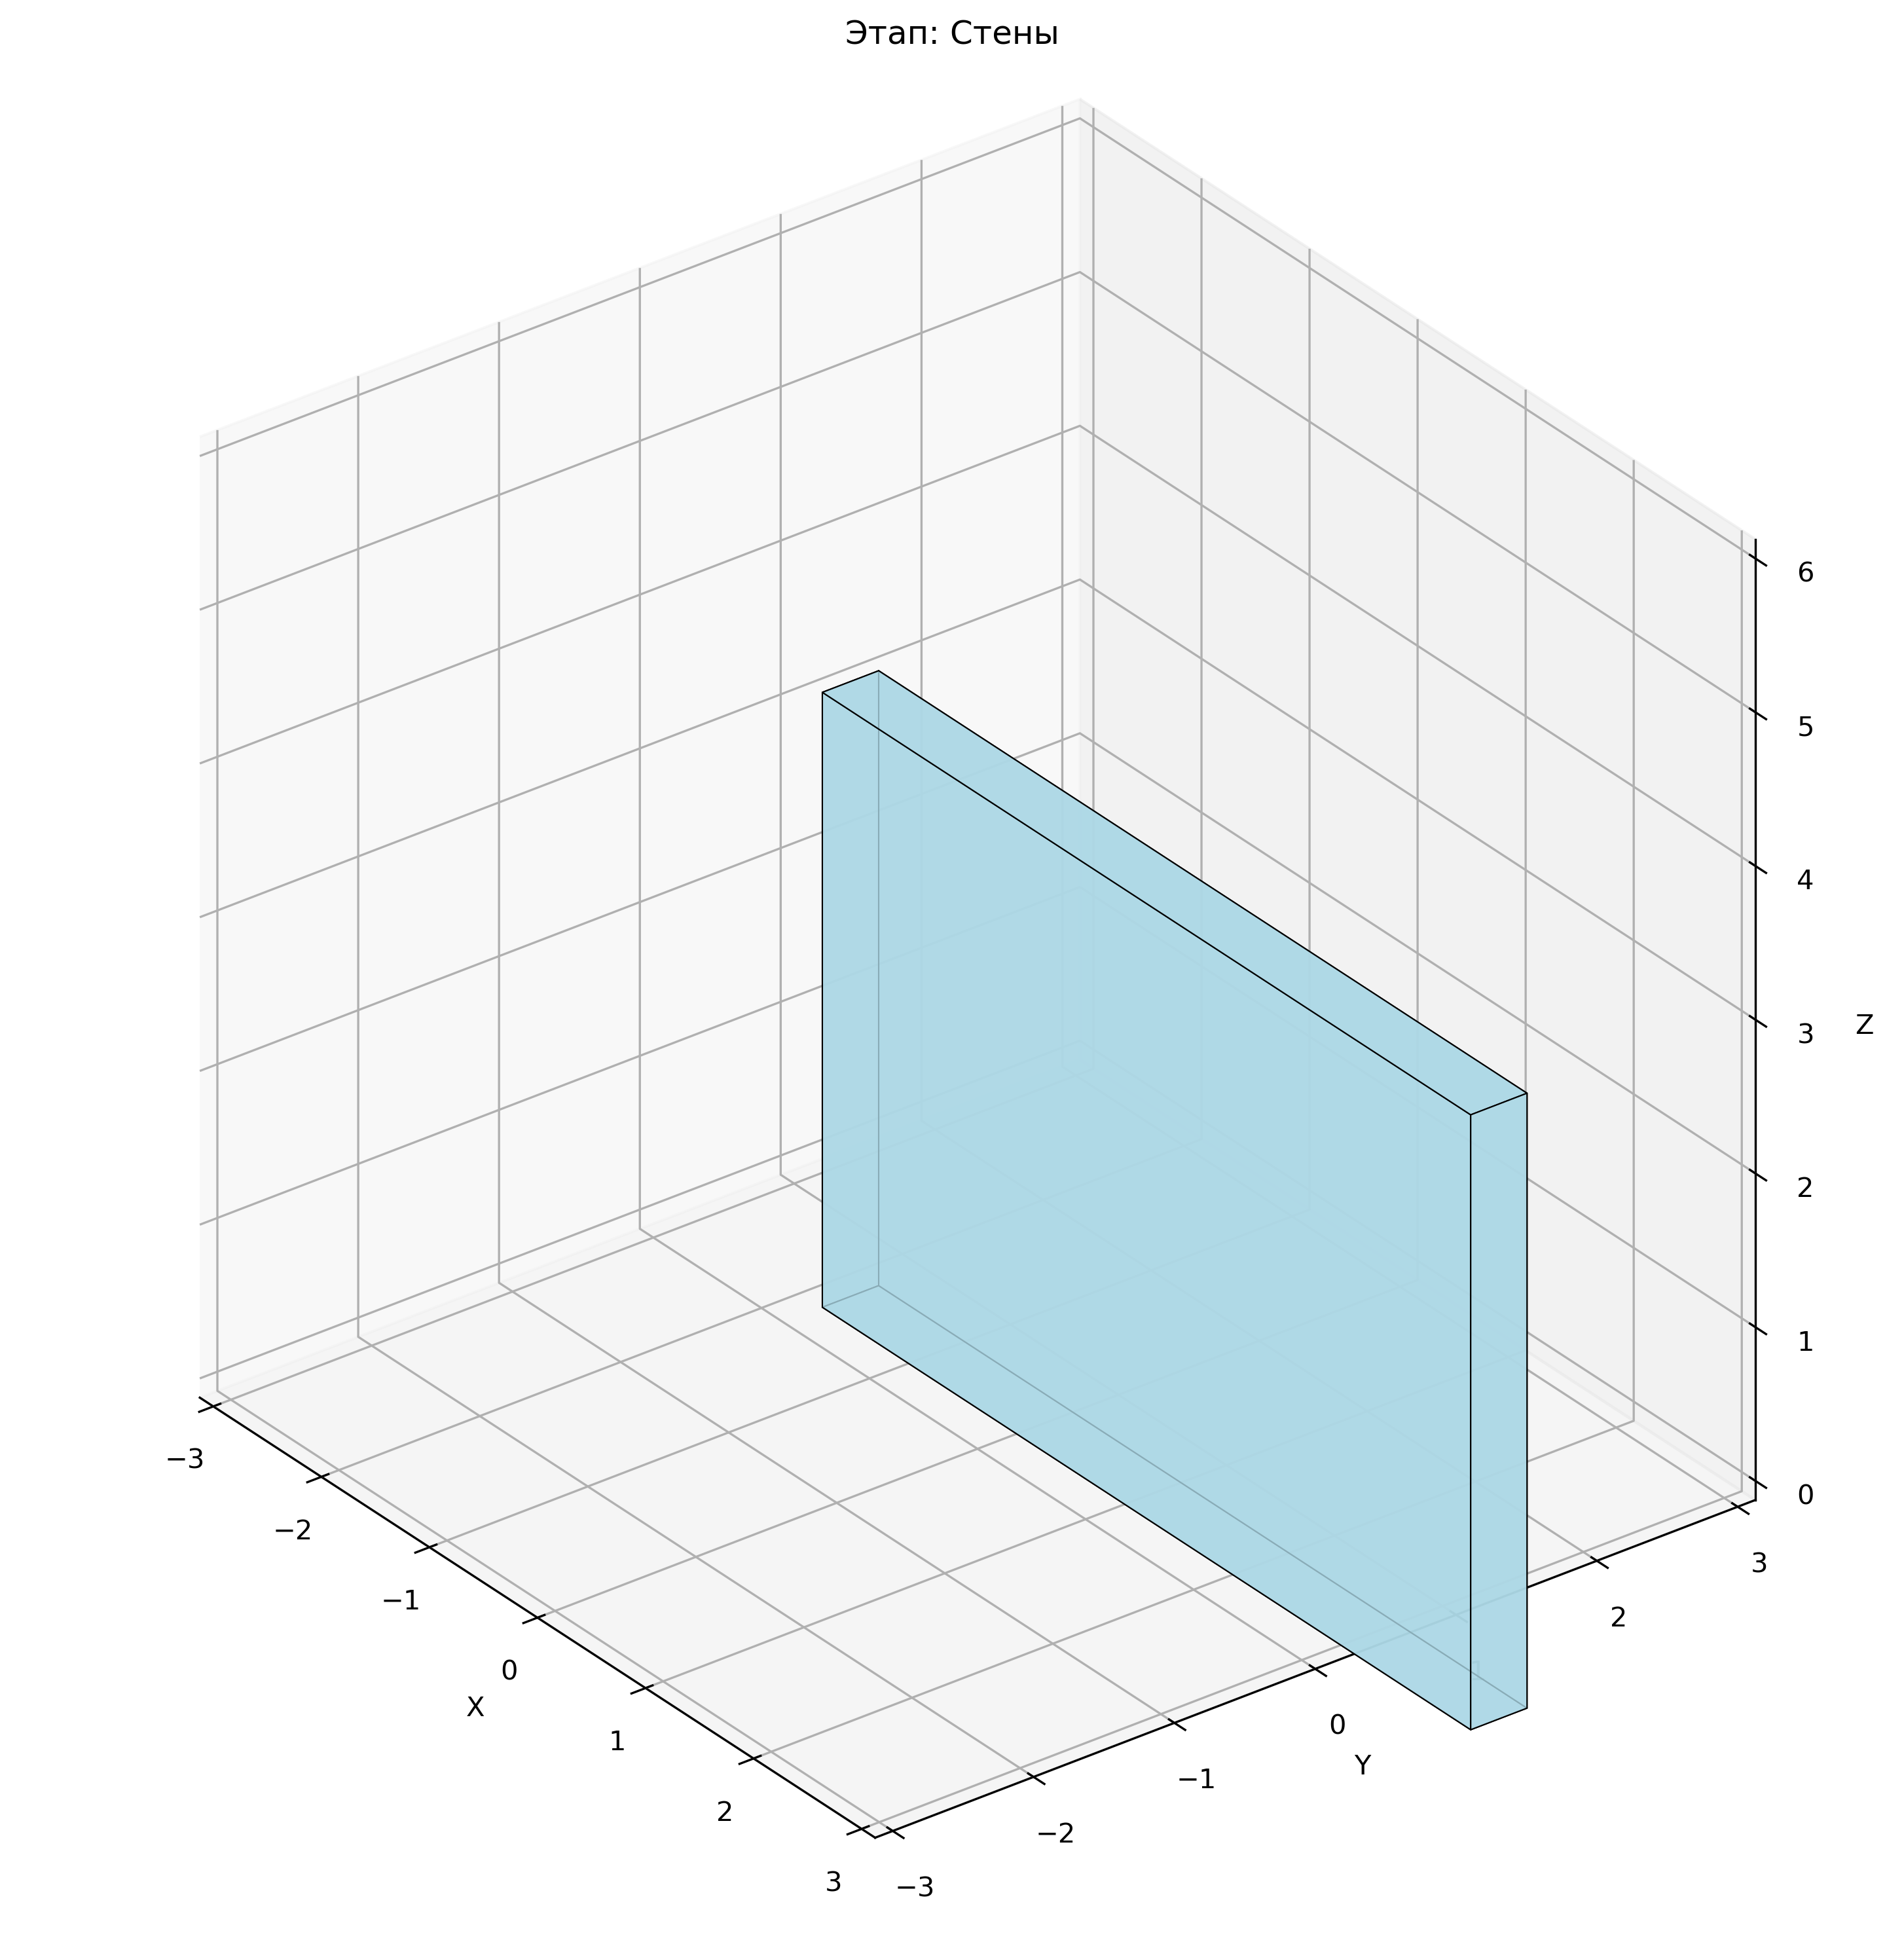
\includegraphics[width=0.8\textwidth]{images/task8/construction_стены.png}
\caption{Этап 2: Стены}
\end{figure}

\begin{figure}[H]
\centering
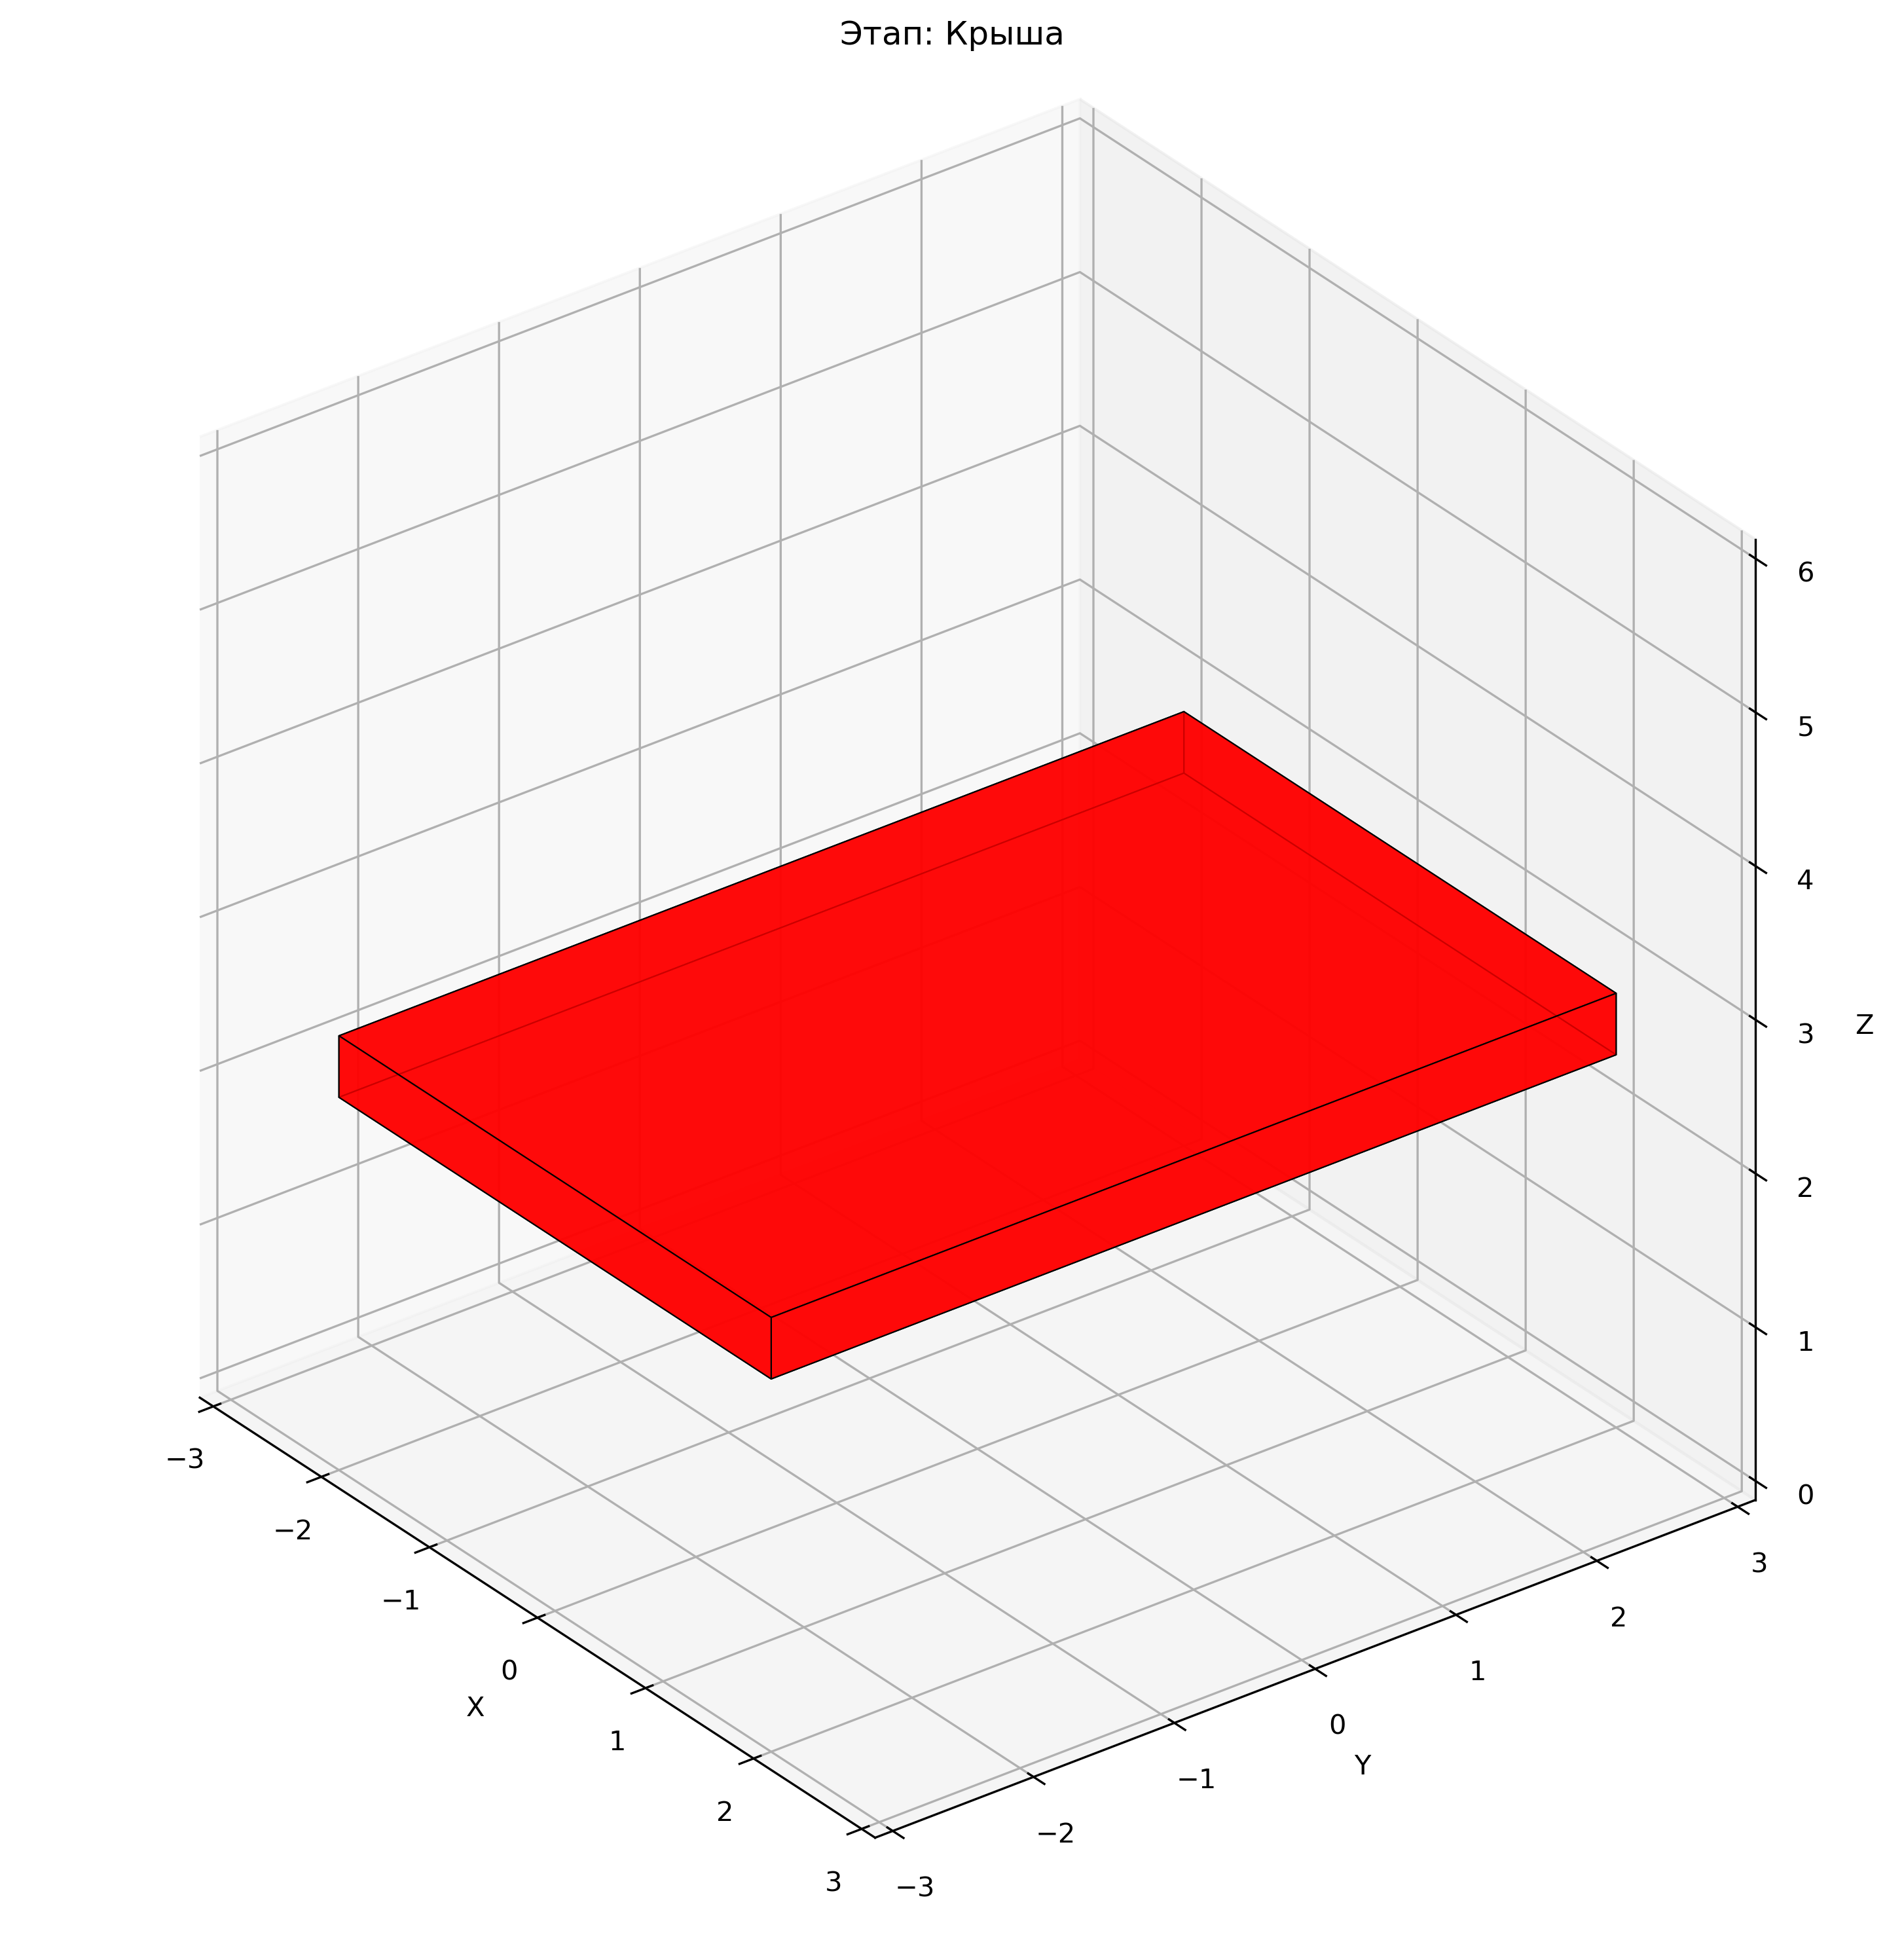
\includegraphics[width=0.8\textwidth]{images/task8/construction_крыша.png}
\caption{Этап 3: Крыша}
\end{figure}

\begin{figure}[H]
\centering
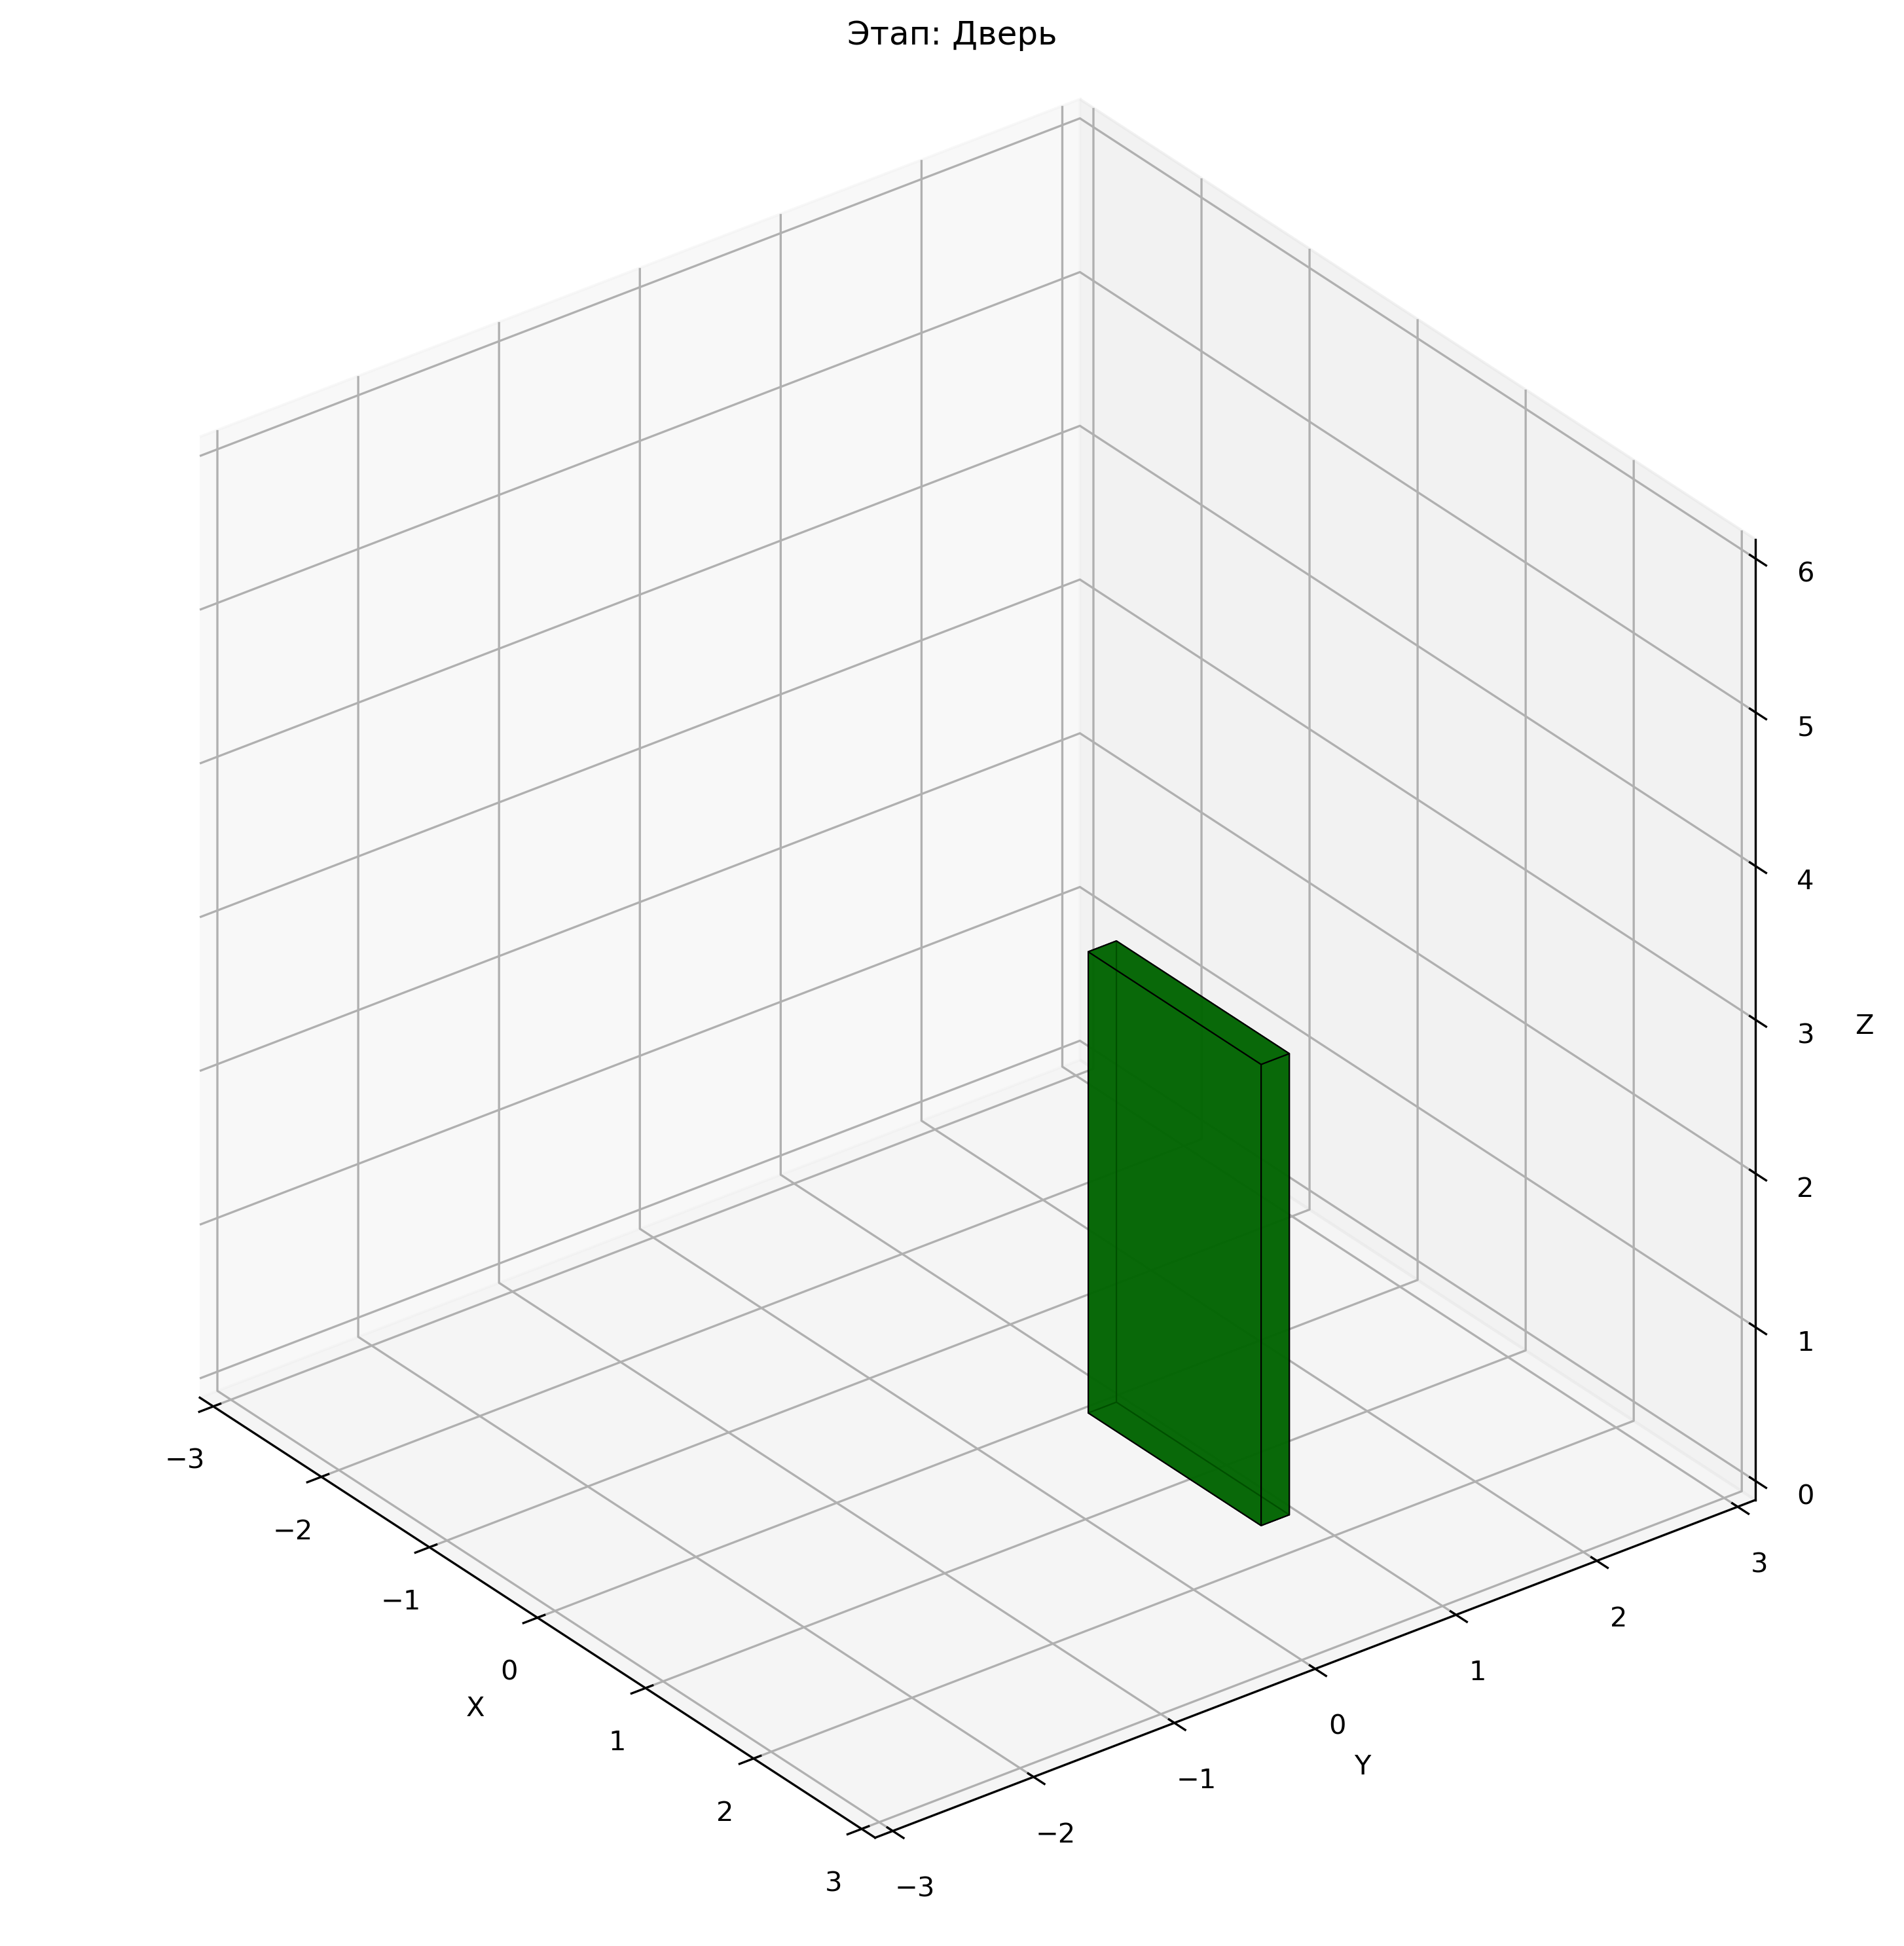
\includegraphics[width=0.8\textwidth]{images/task8/construction_дверь.png}
\caption{Этап 4: Дверь}
\end{figure}

\begin{figure}[H]
\centering
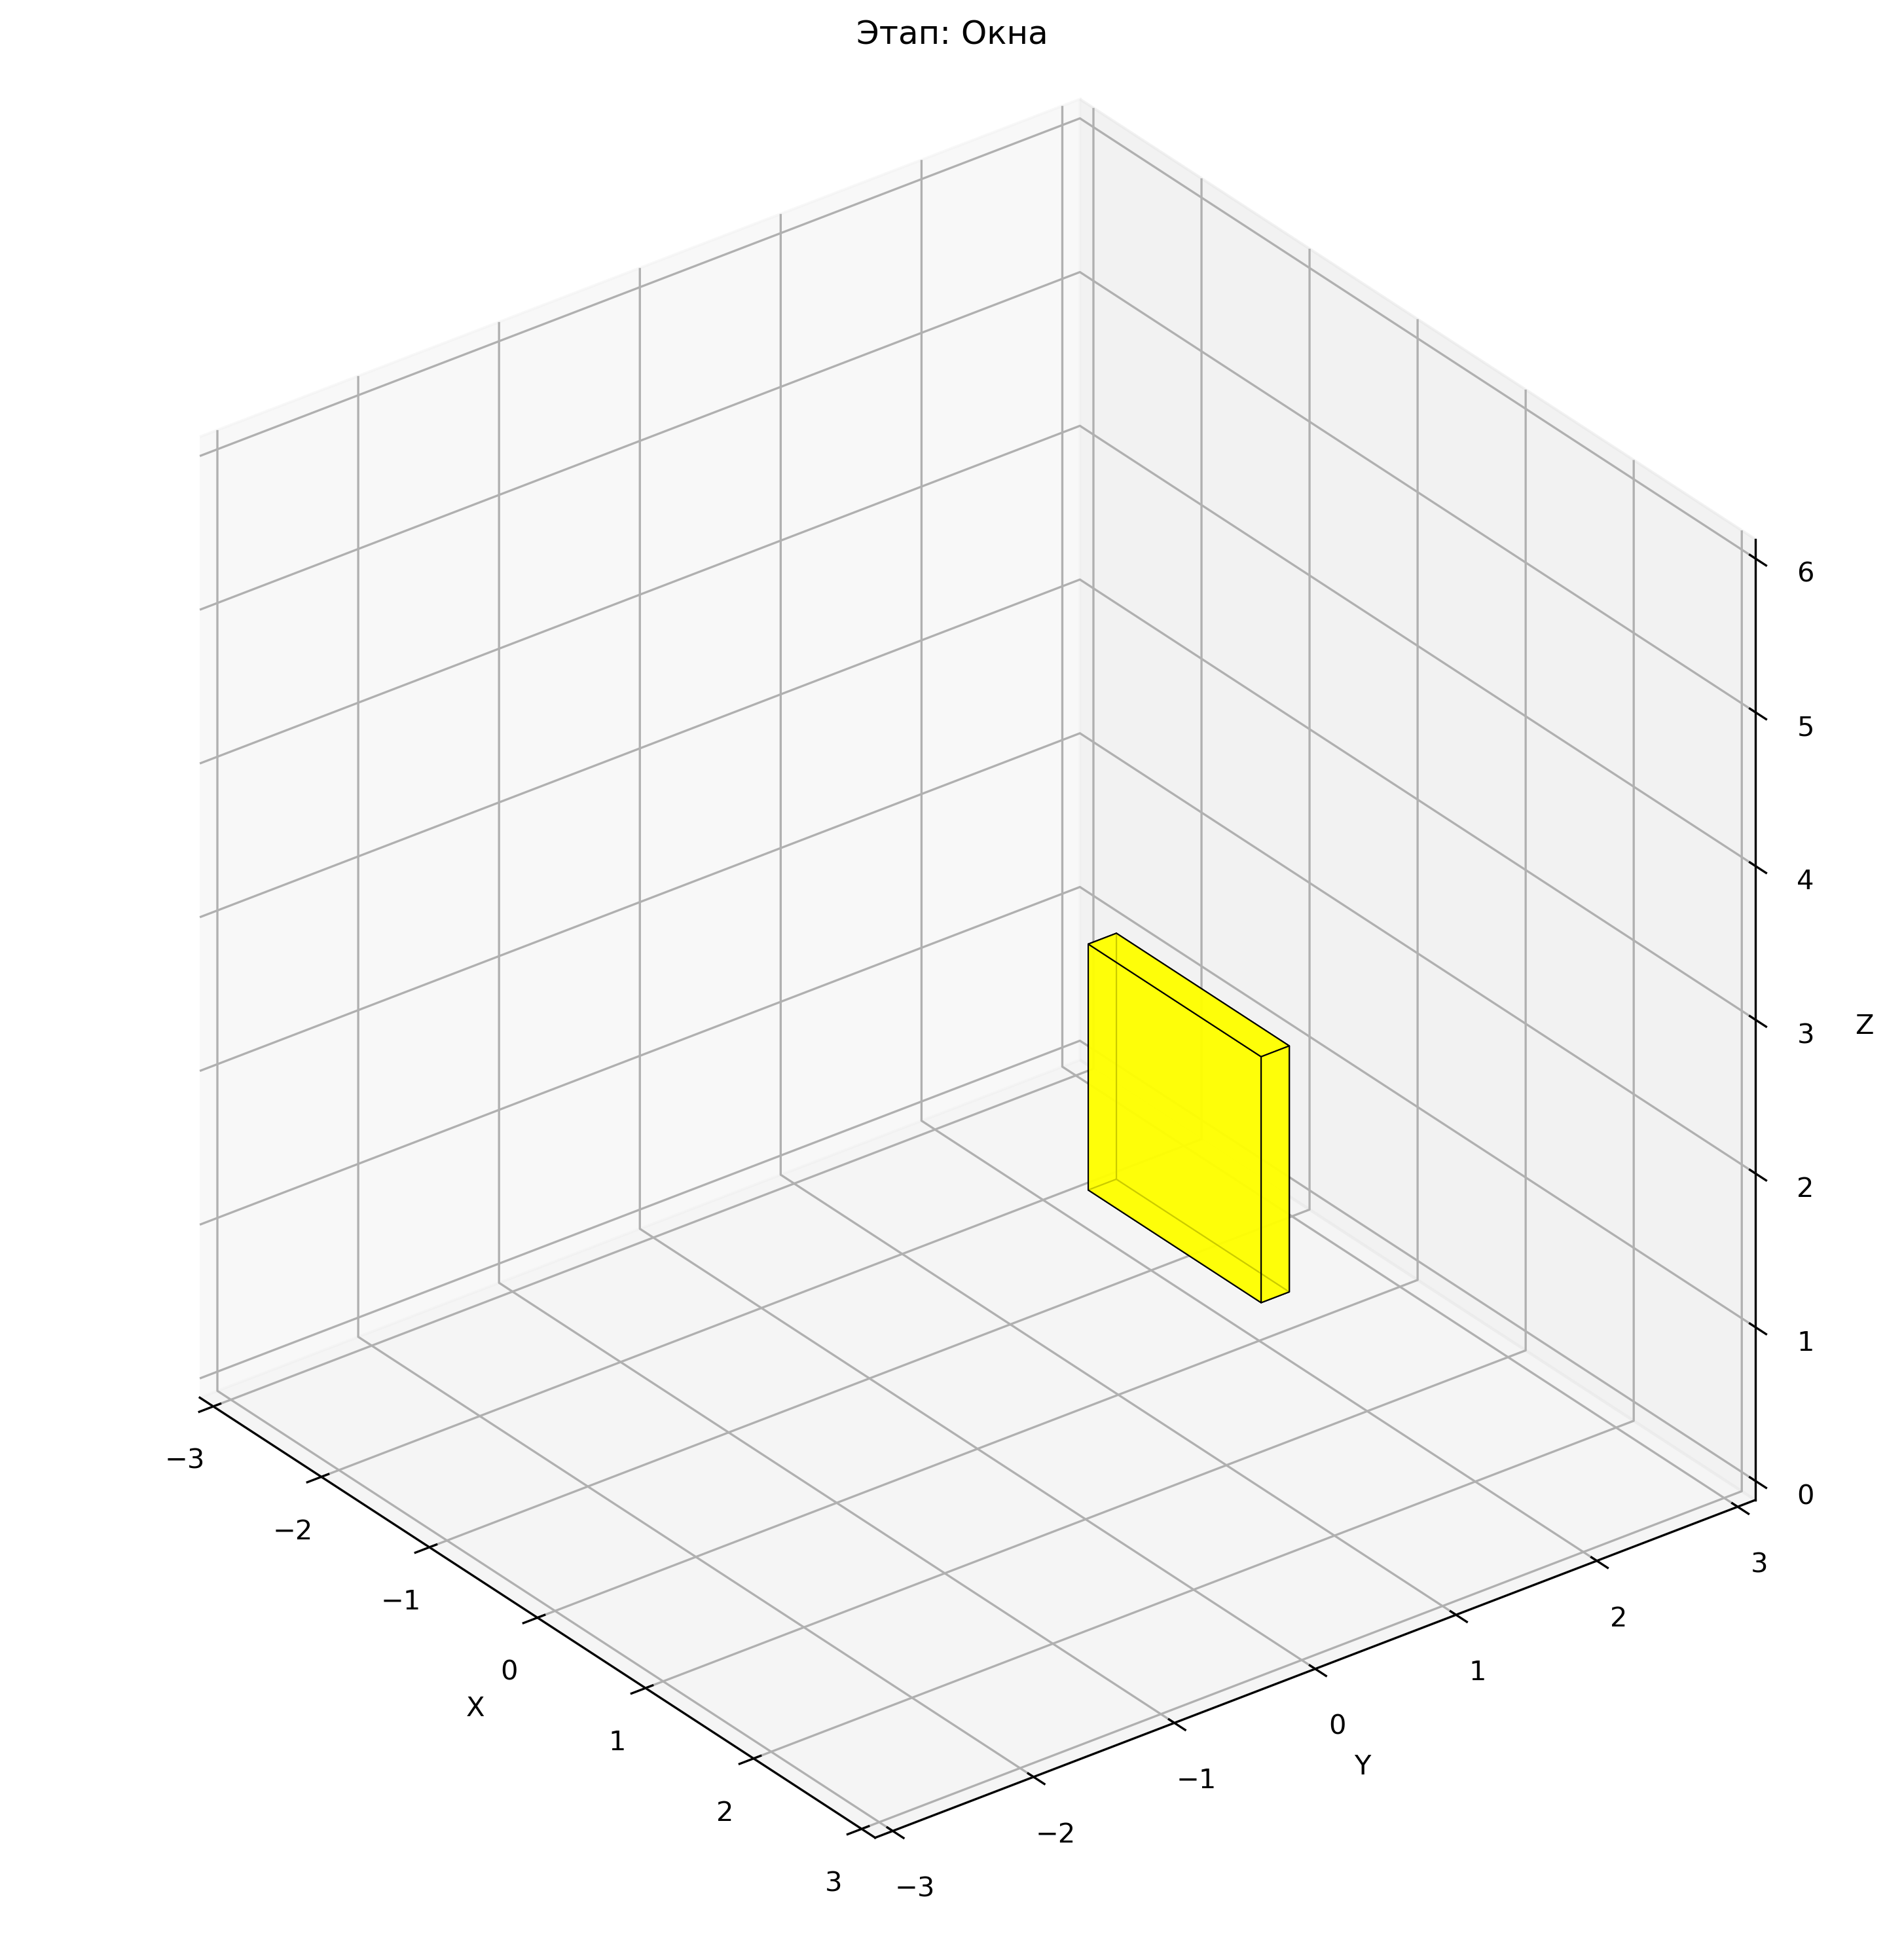
\includegraphics[width=0.8\textwidth]{images/task8/construction_окна.png}
\caption{Этап 5: Окна}
\end{figure}

\begin{figure}[H]
\centering
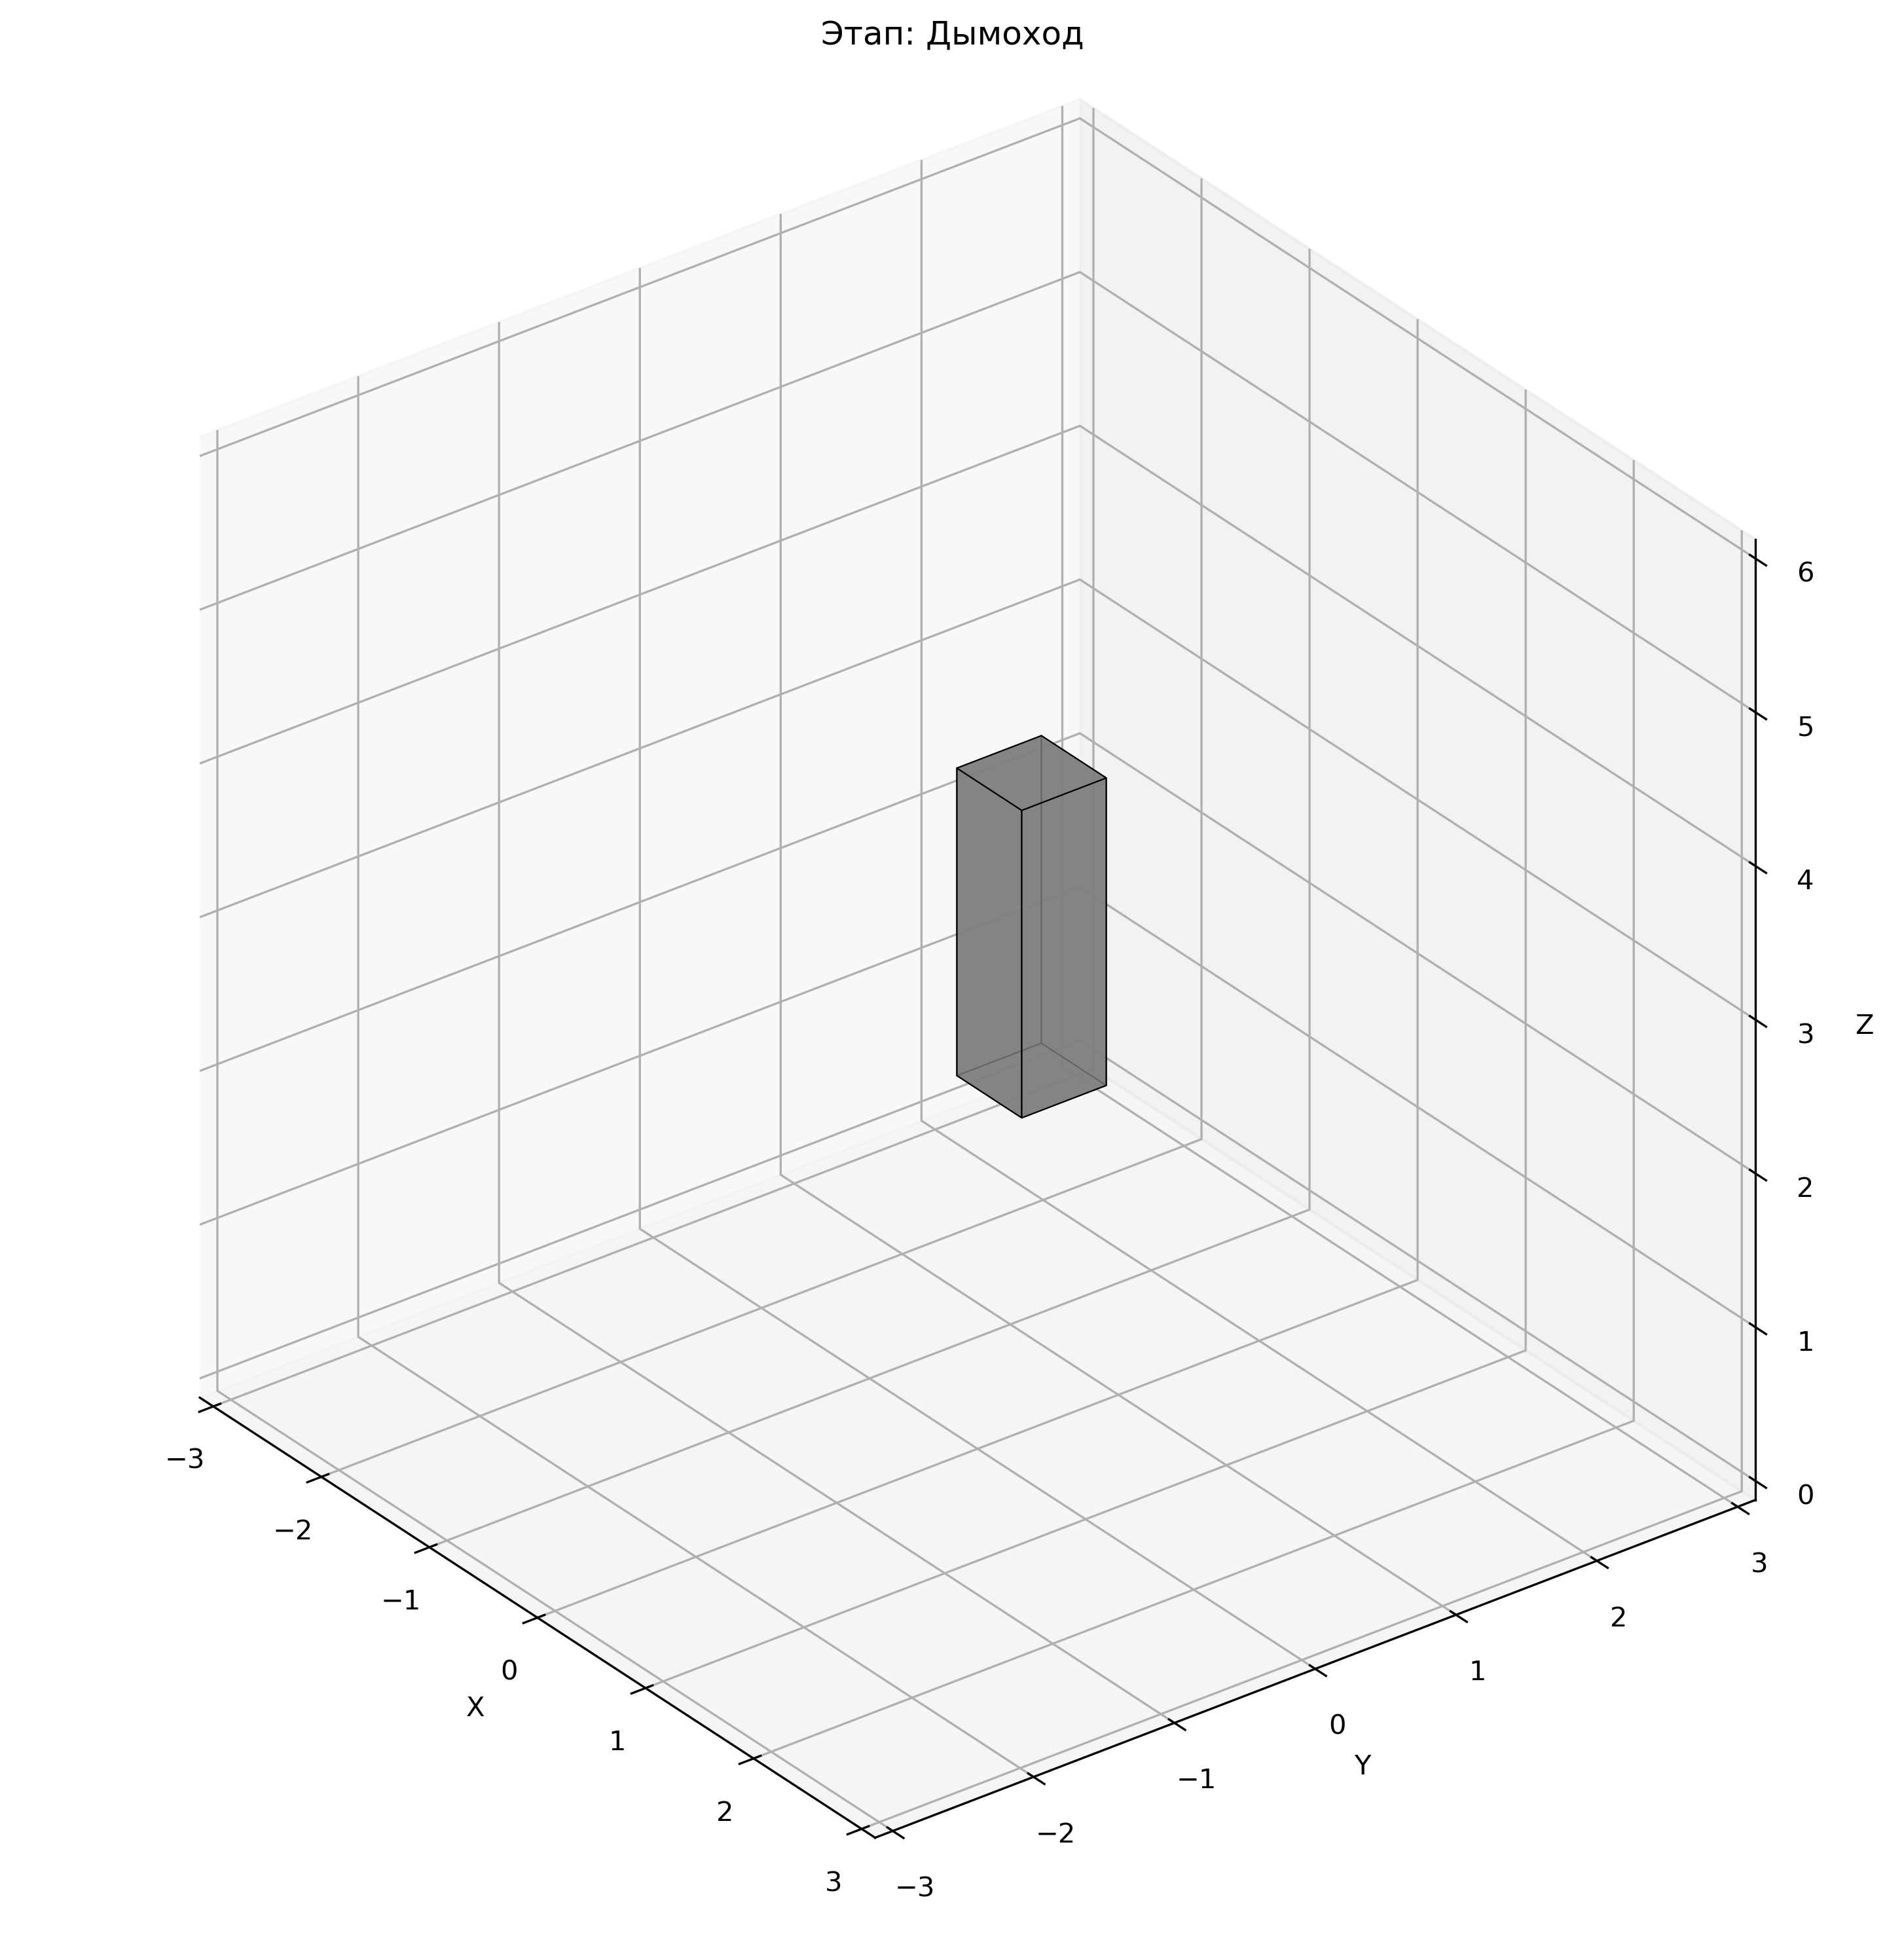
\includegraphics[width=0.8\textwidth]{images/task8/construction_дымоход.png}
\caption{Этап 6: Дымоход}
\end{figure}

\subsection*{Виды домика с разных углов}

\begin{figure}[H]
\centering
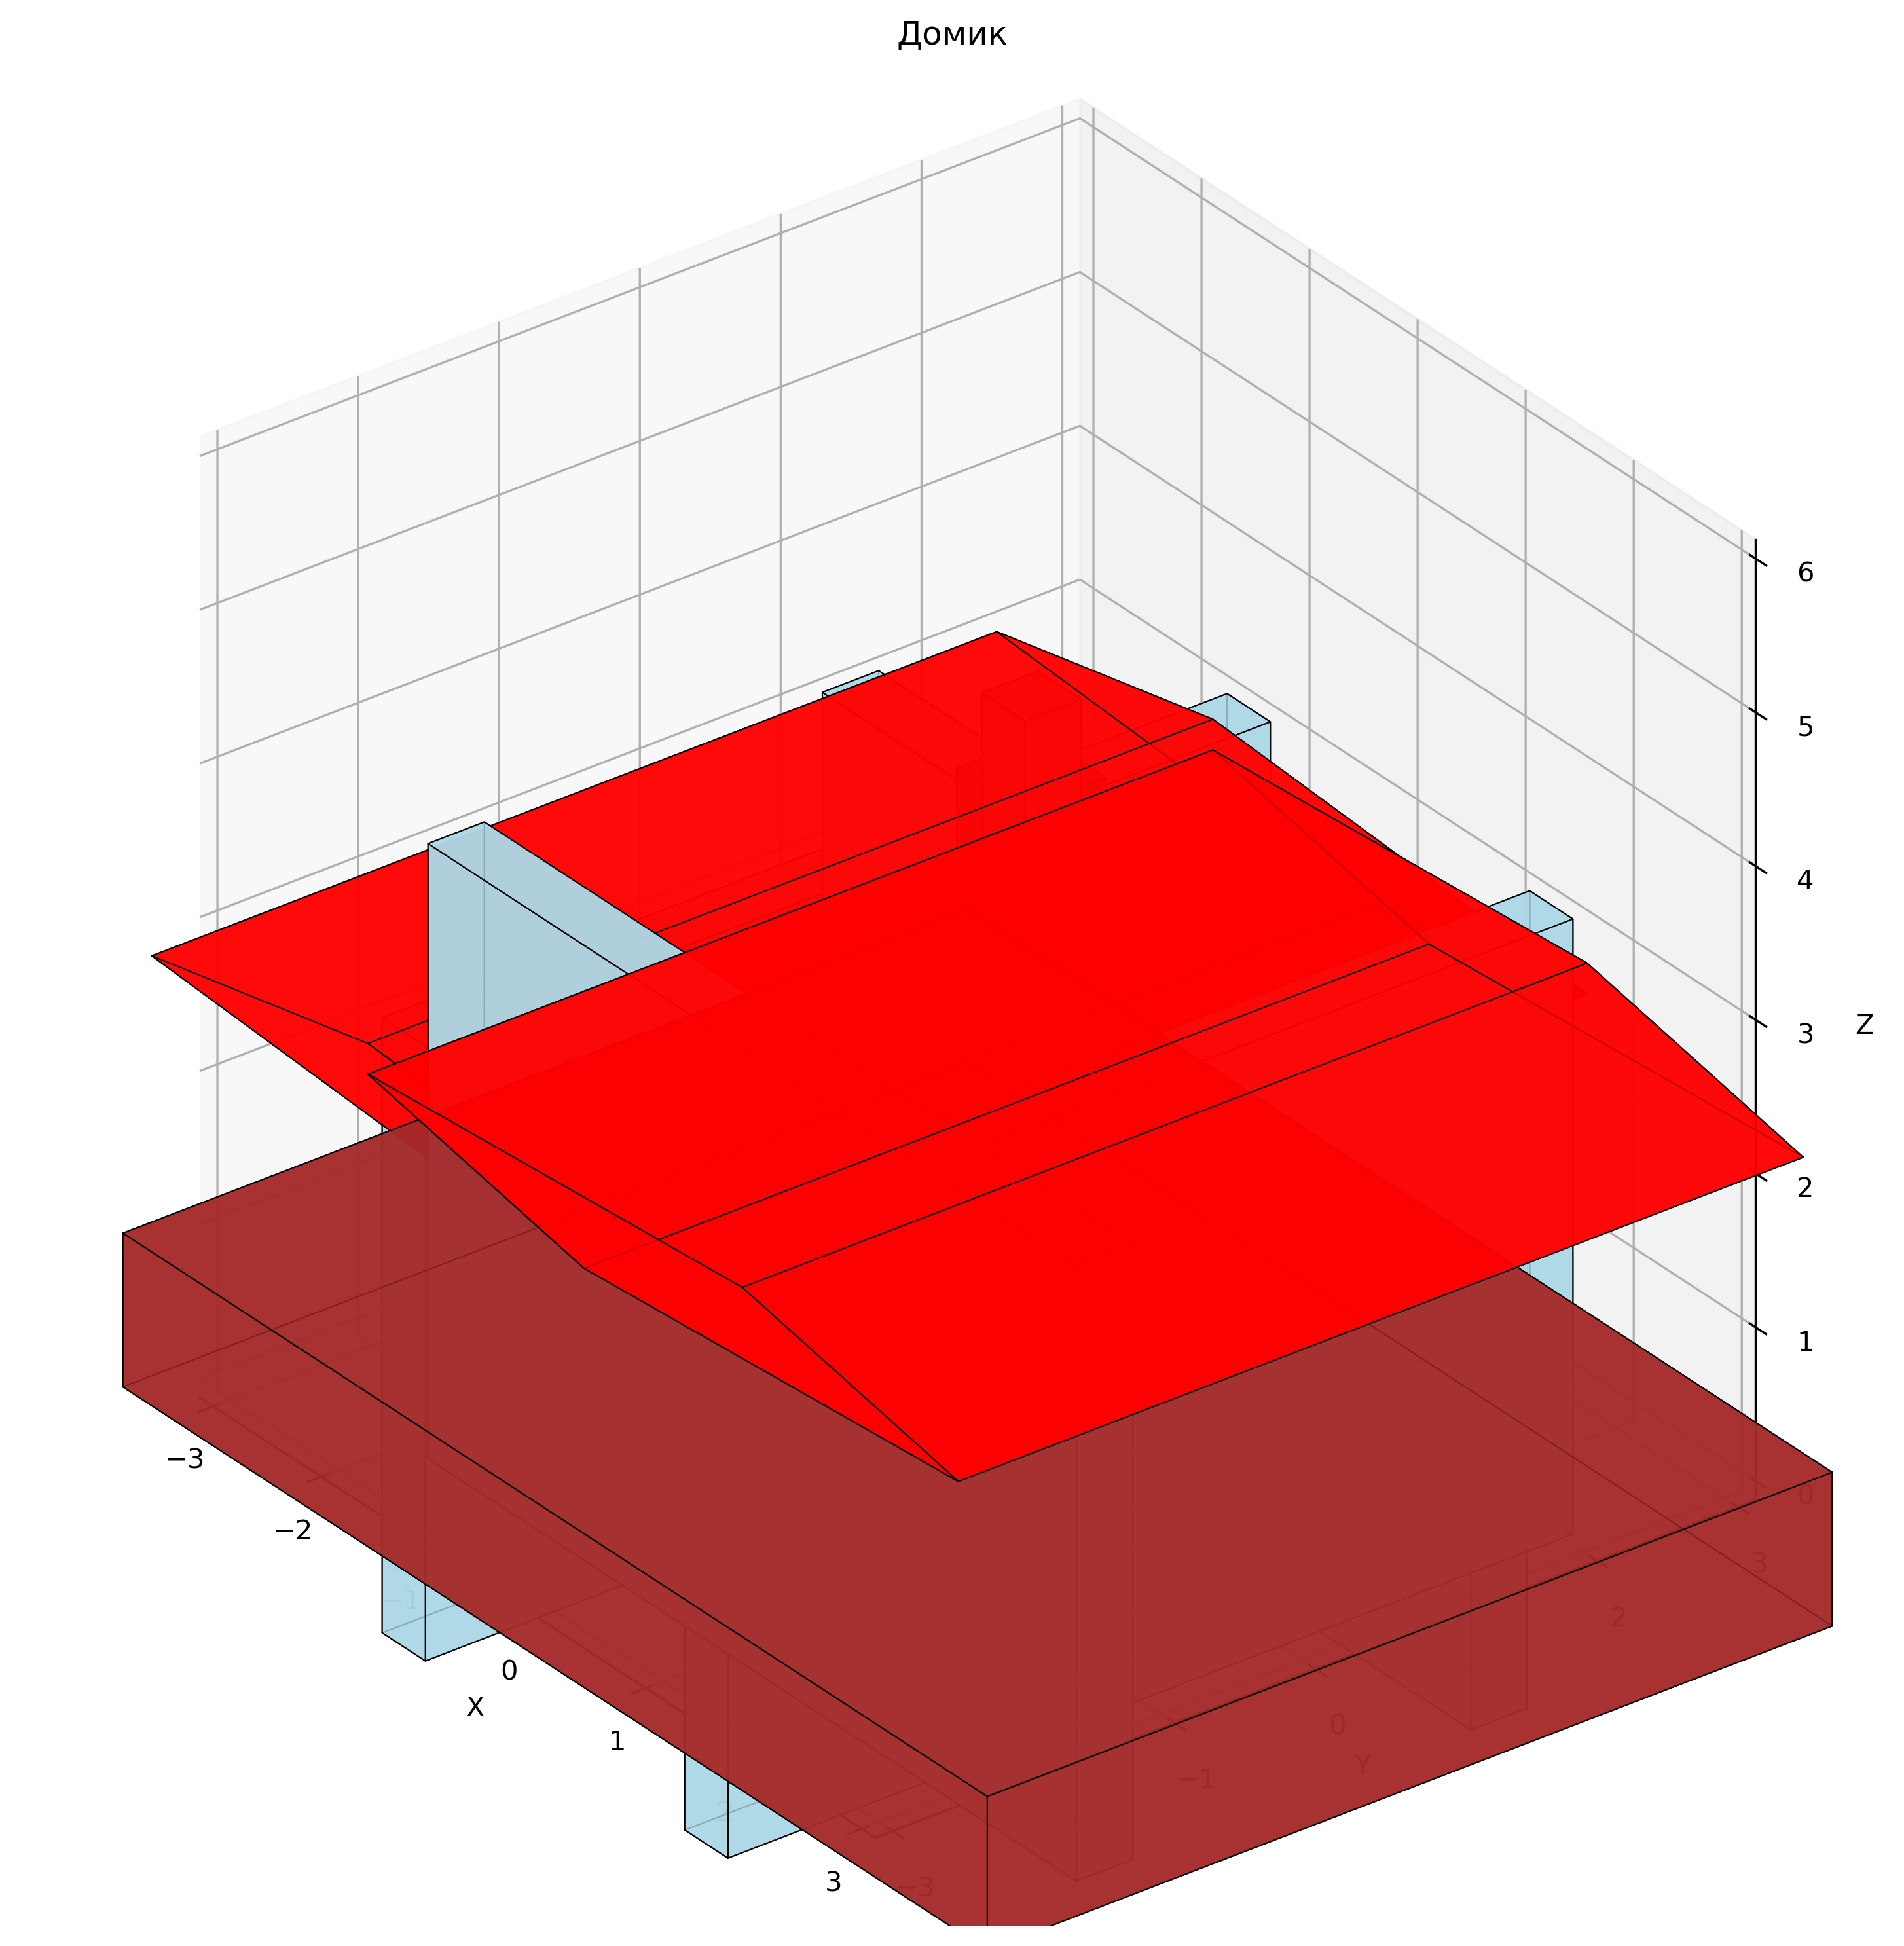
\includegraphics[width=0.8\textwidth]{images/task8/house_original.png}
\caption{Исходный вид домика}
\end{figure}

\begin{figure}[H]
\centering
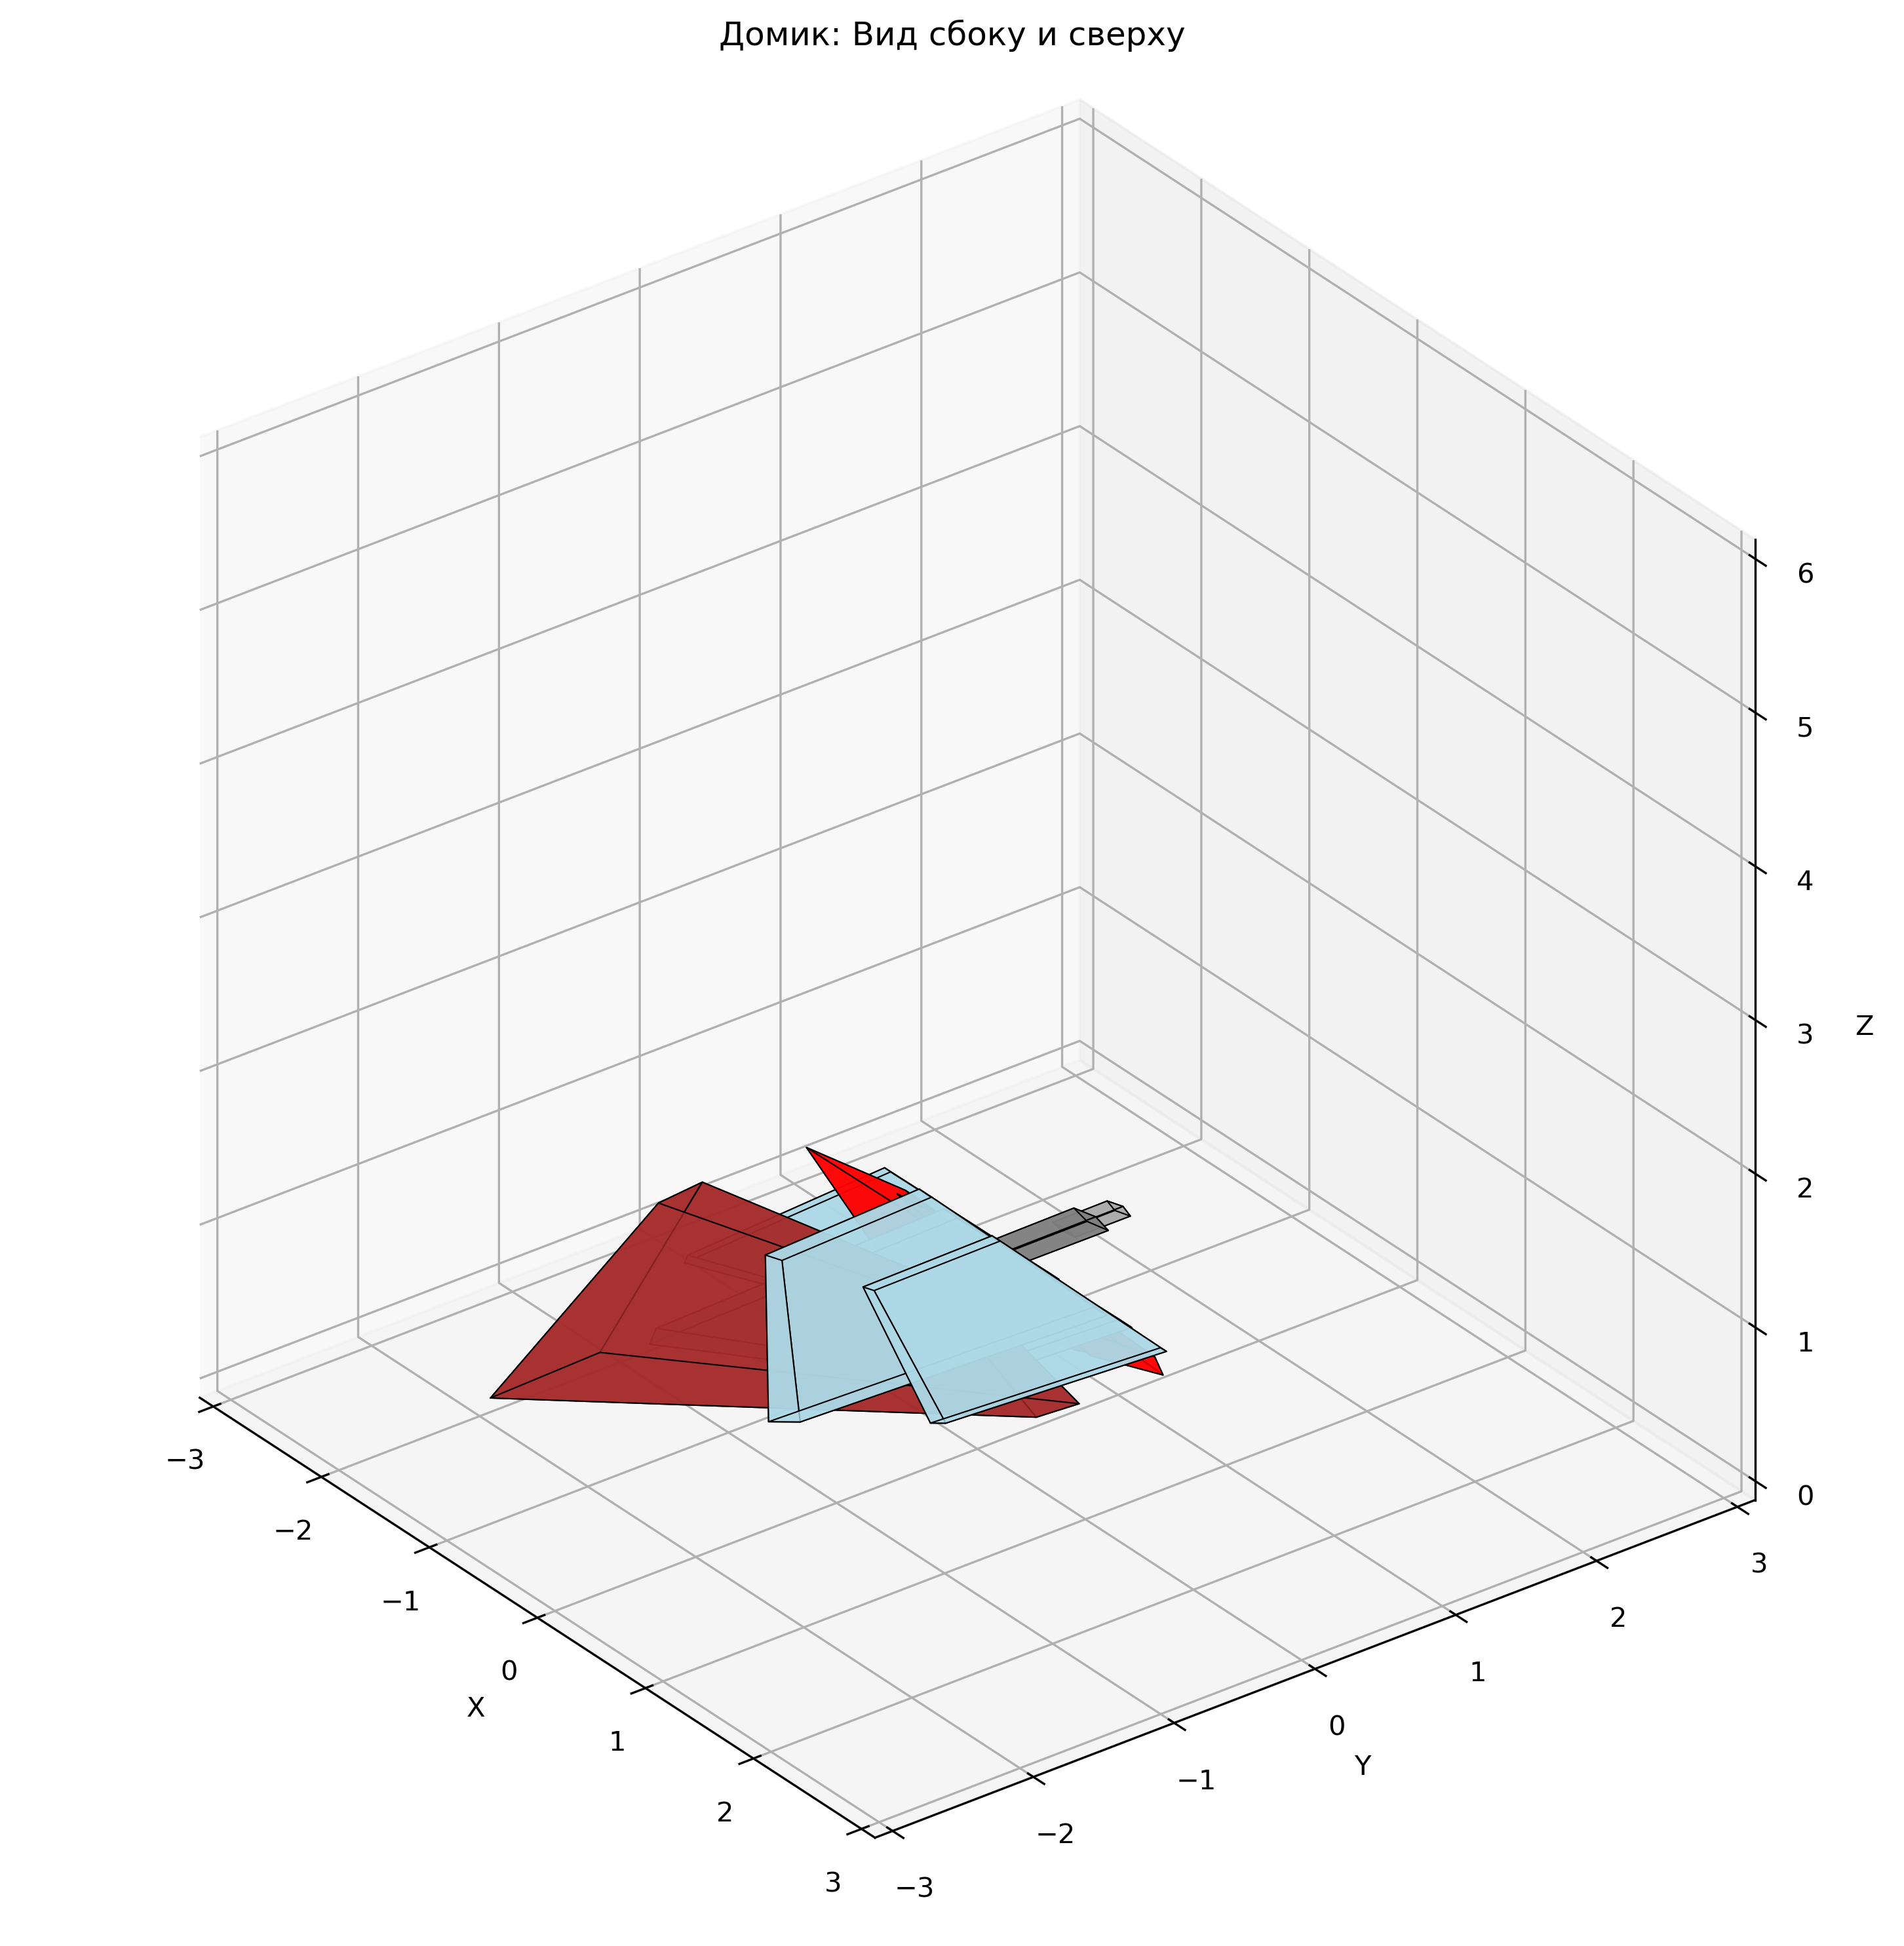
\includegraphics[width=0.8\textwidth]{images/task8/house_side_top.png}
\caption{Вид сбоку и сверху}
\end{figure}

\begin{figure}[H]
\centering
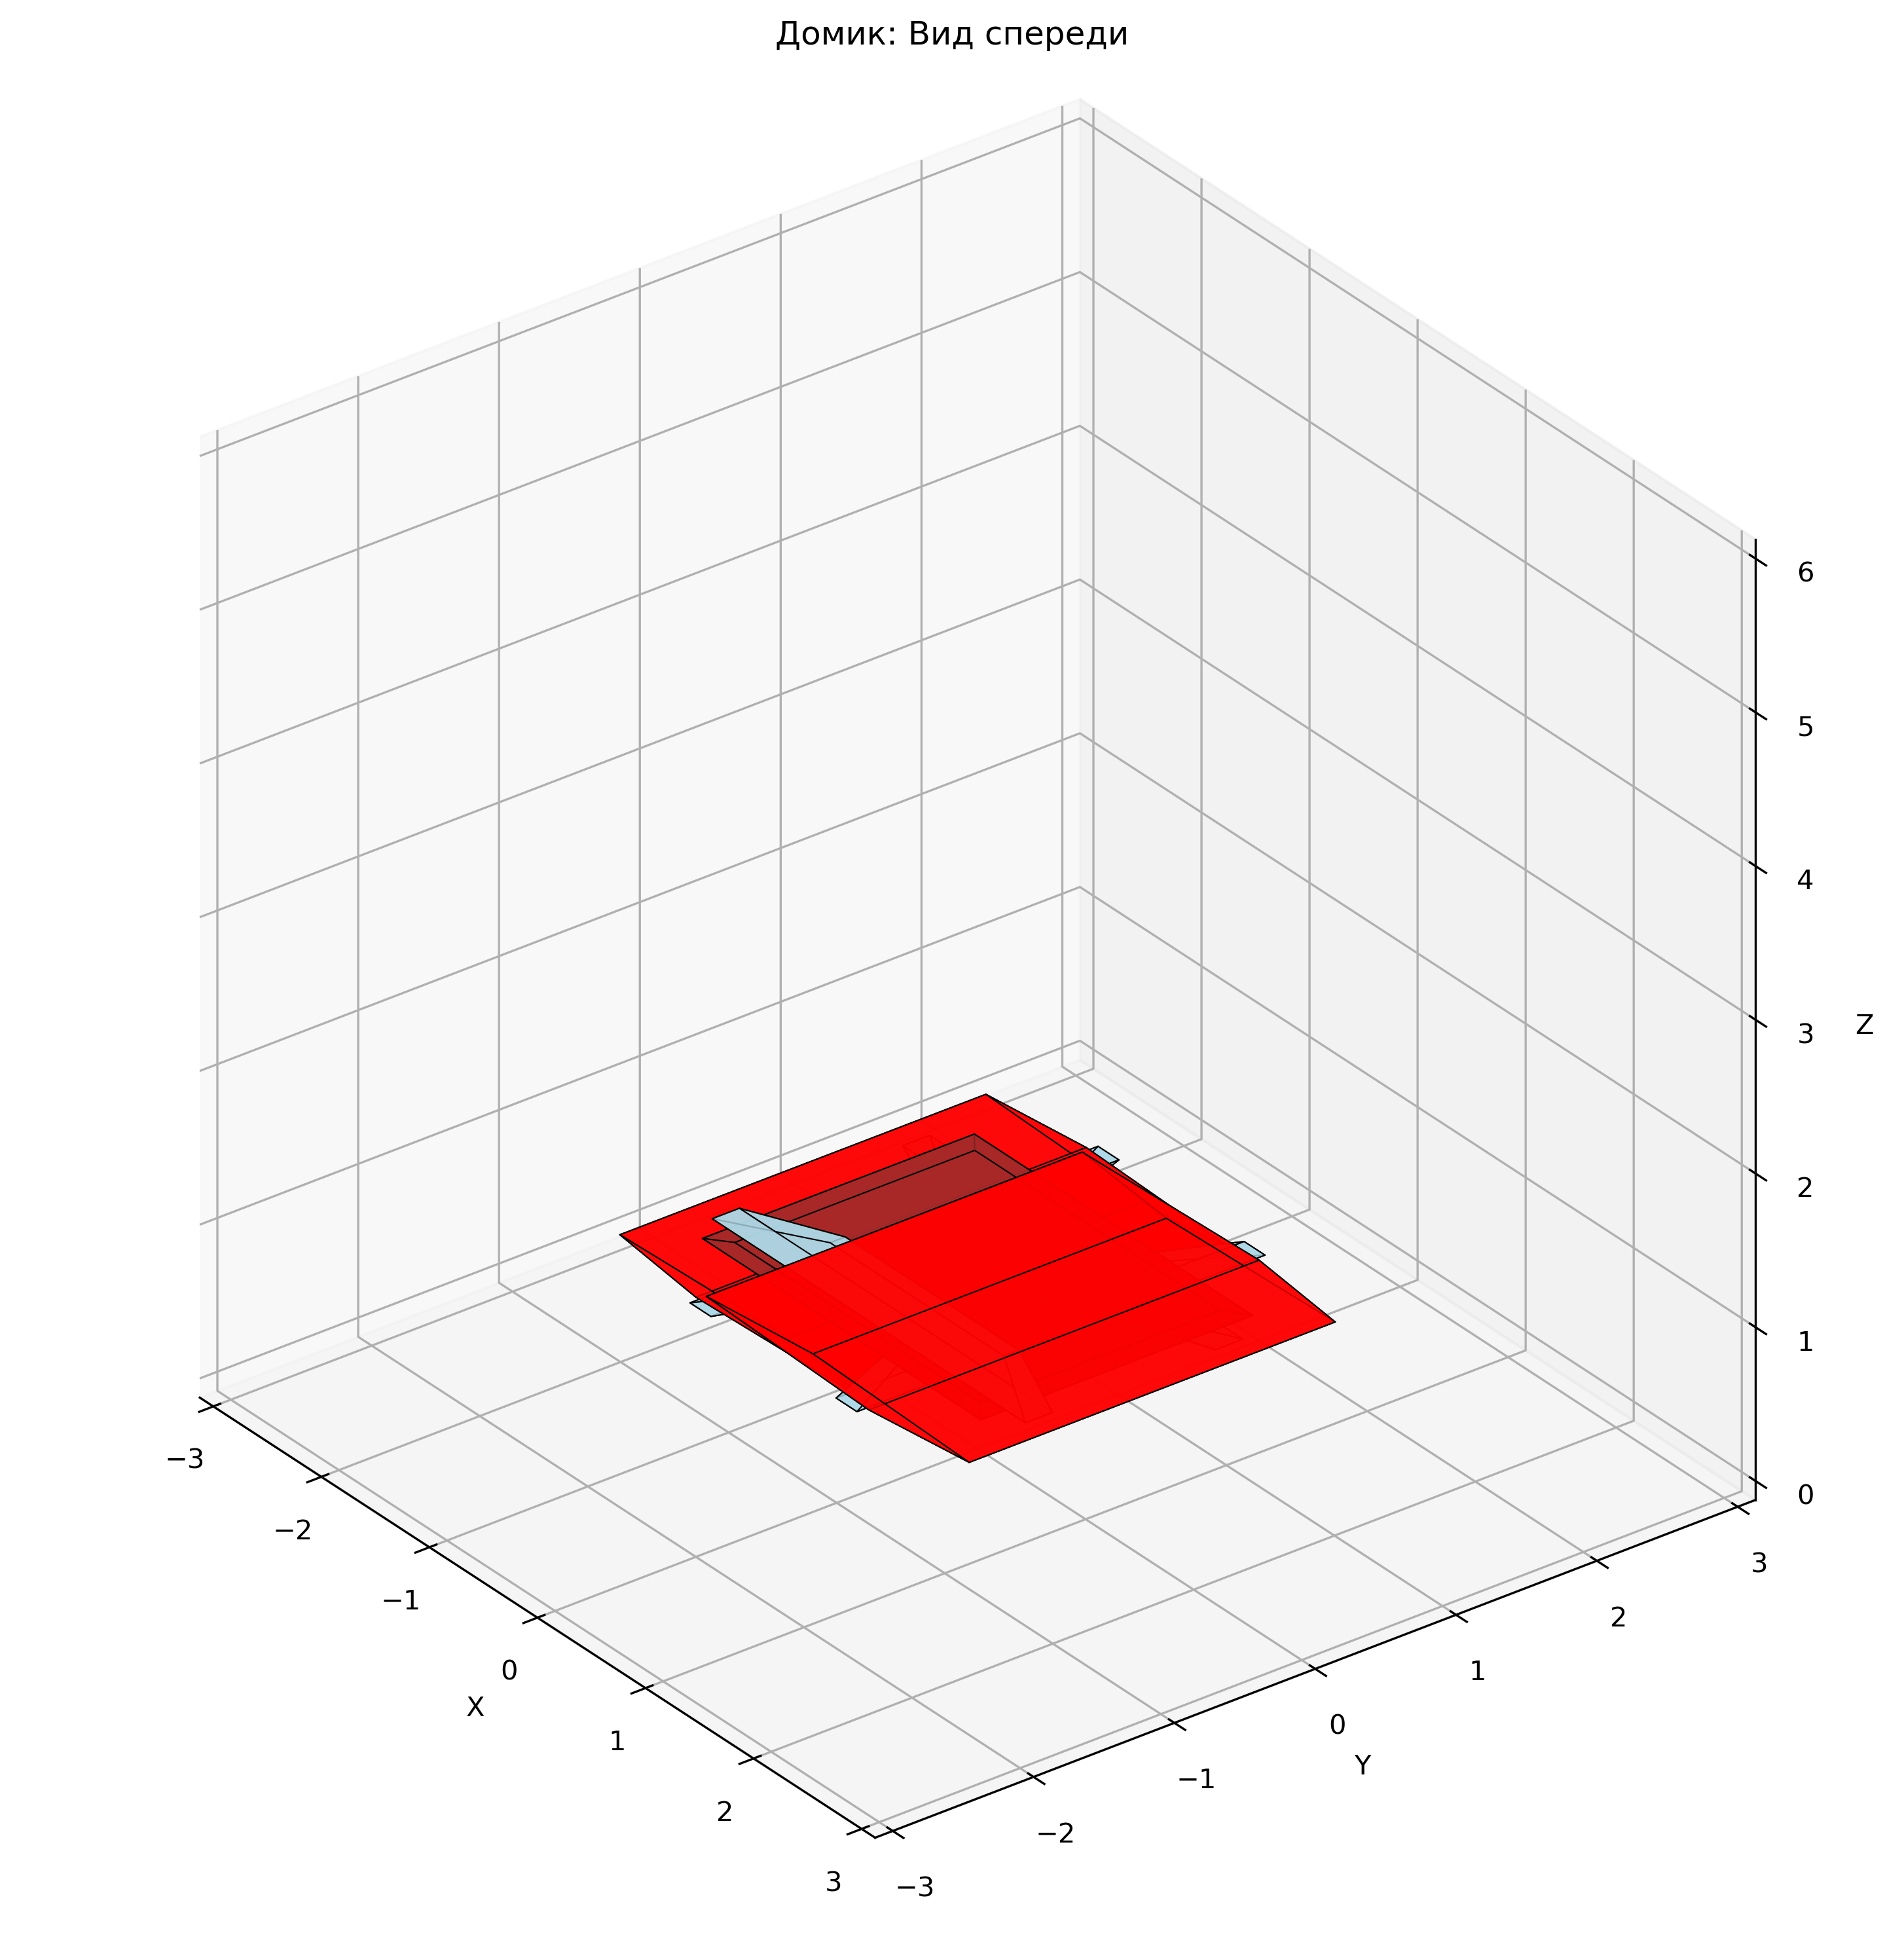
\includegraphics[width=0.8\textwidth]{images/task8/house_front.png}
\caption{Вид спереди}
\end{figure}

\begin{figure}[H]
\centering
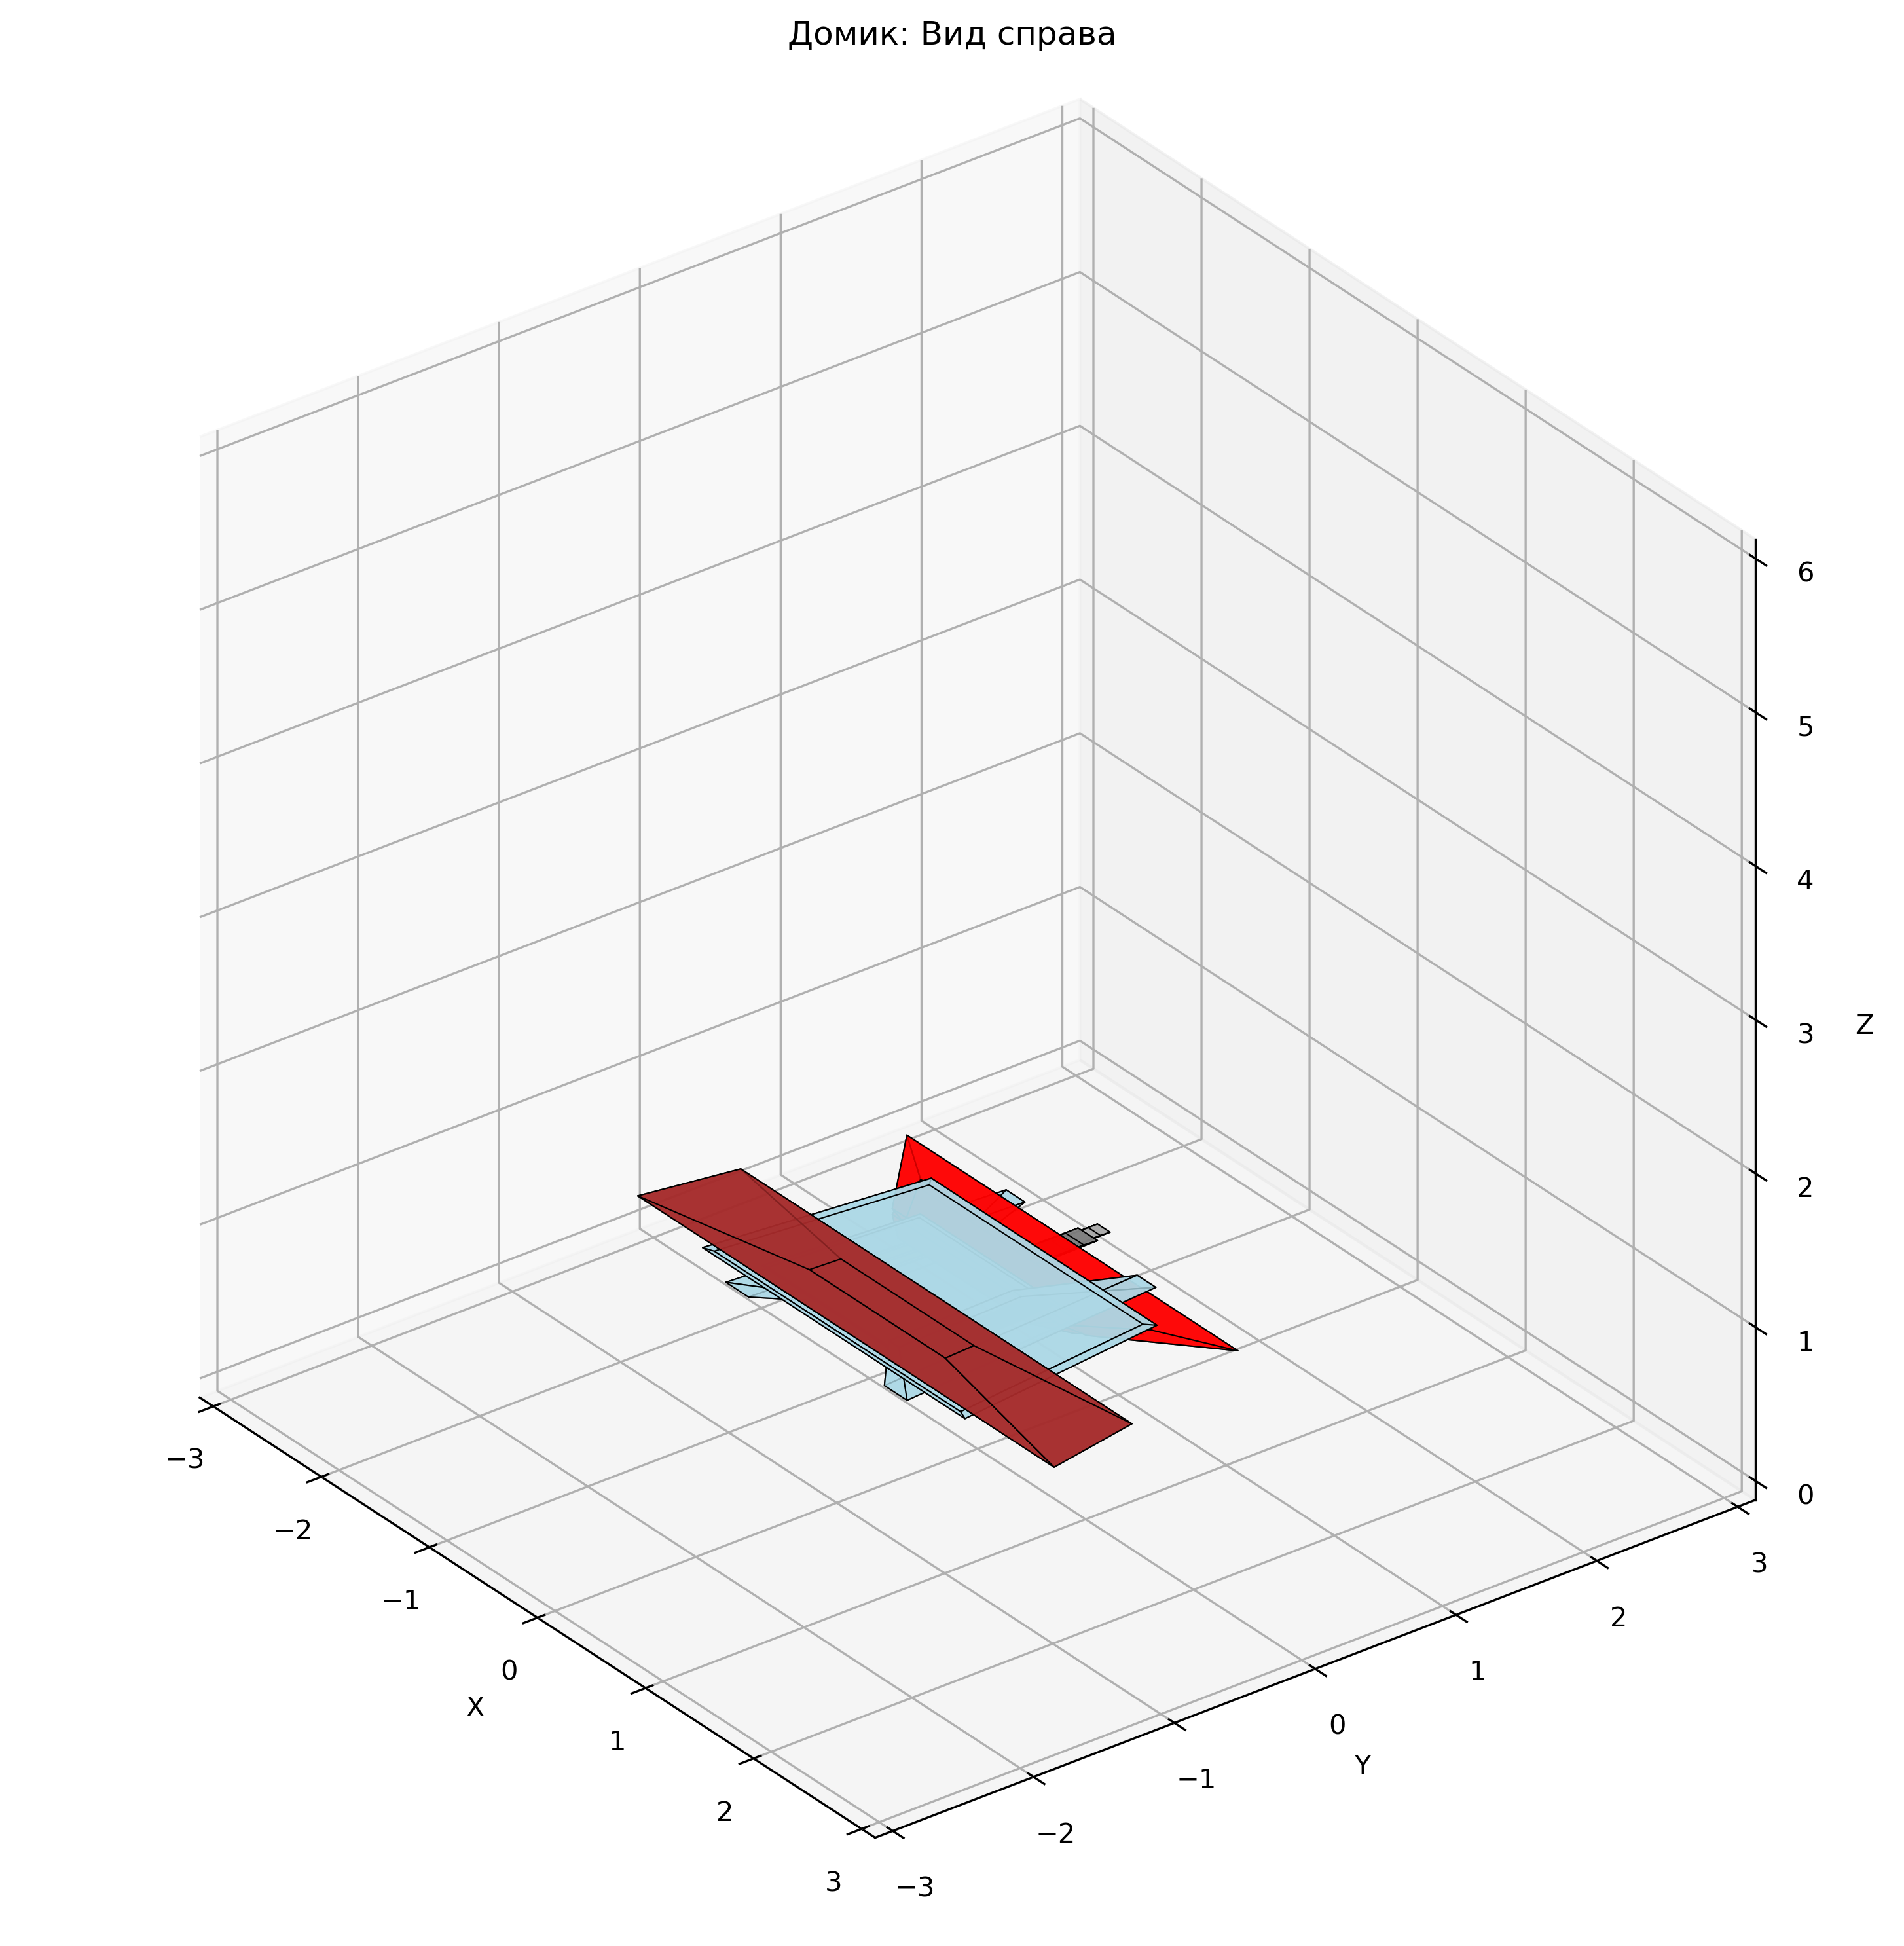
\includegraphics[width=0.8\textwidth]{images/task8/house_right.png}
\caption{Вид справа}
\end{figure}

\begin{figure}[H]
\centering
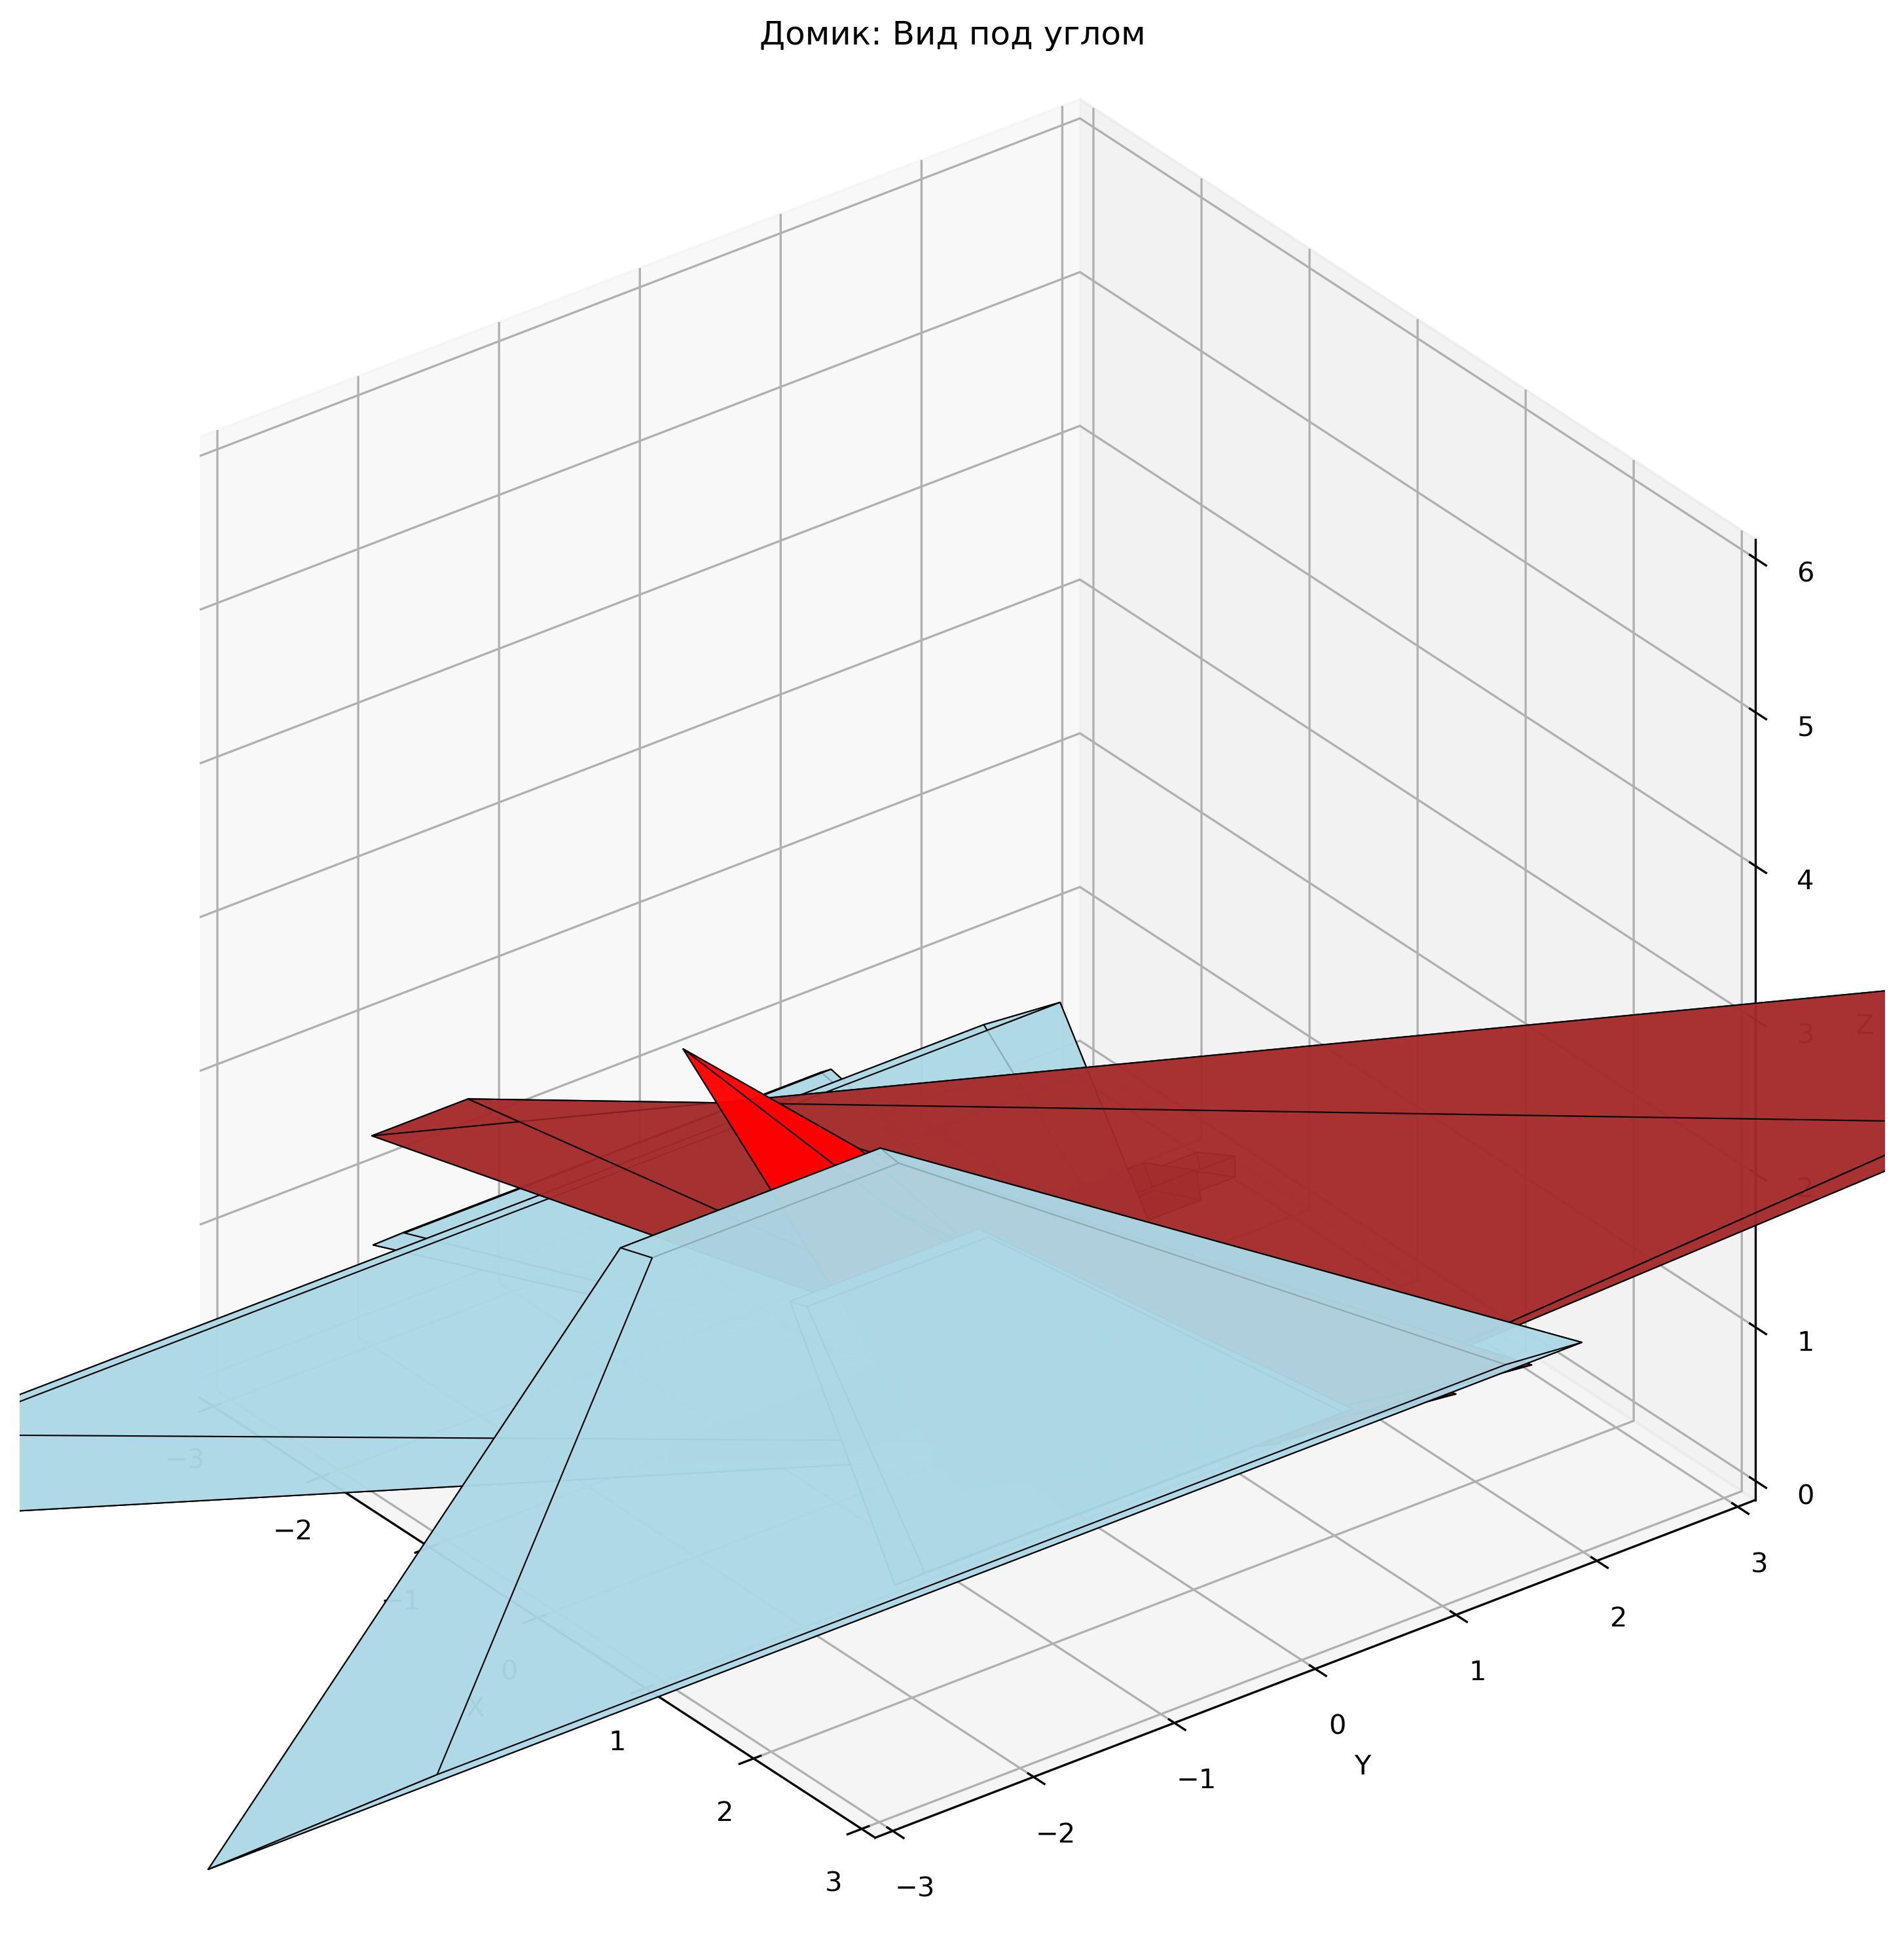
\includegraphics[width=0.8\textwidth]{images/task8/house_angle.png}
\caption{Вид под углом}
\end{figure}

\subsection*{Статистика домика}
\begin{itemize}
    \item Количество элементов: 12
    \item Общий объем: 115.47 кубических единиц
    \item Использованы все типы преобразований: масштабирование, перемещение, вращение
    \item Каждый элемент имеет свой цвет и назначение
\end{itemize}

\section*{Общий анализ и выводы}

\subsection*{Достигнутые результаты}
\begin{enumerate}
    \item Успешно реализованы все основные аффинные преобразования в 3D
    \item Исследованы свойства и композиции преобразований
    \item Демонстрирована работа с однородными координатами
    \item Реализована камера с различными позициями и ориентациями
    \item Исследованы перспективные преобразования
    \item Создана сложная 3D сцена (домик) с использованием всех изученных техник
\end{enumerate}

\subsection*{Ключевые выводы}
\begin{itemize}
    \item Однородные координаты необходимы для представления аффинных преобразований в матричном виде
    \item Преобразования масштабирования и перемещения не коммутируют
    \item Любое вращение в 3D можно представить как вращение вокруг одной оси (теорема Эйлера)
    \item Камера позволяет изменять точку зрения на сцену
    \item Перспективные преобразования создают реалистичное изображение глубины
    \item Композиция преобразований позволяет создавать сложные 3D сцены
\end{itemize}

\subsection*{Практическое применение}
Полученные знания и навыки могут быть применены в:
\begin{itemize}
    \item Компьютерной графике и анимации
    \item Разработке игр
    \item Системах автоматизированного проектирования (CAD)
    \item Робототехнике и кинематике
    \item Компьютерном зрении
\end{itemize}

\section*{Заключение}

Лабораторная работа успешно выполнена. Все поставленные задачи решены, включая создание базовых геометрических объектов, реализацию основных аффинных преобразований, исследование их свойств и композиций, а также создание сложной 3D сцены. Полученные результаты демонстрируют глубокое понимание математических основ компьютерной графики и готовность к применению этих знаний в практических задачах.
